\documentclass{dissert}
\usepackage{cmap}
\usepackage[T2A]{fontenc}
\usepackage[utf8]{inputenc}
\usepackage{tabularx}
\usepackage[noend]{algorithmic}
\usepackage{tikz}
\usepackage{tikz,fullpage}
\usepackage{lastpage}
\usepackage[shortlabels]{enumitem}
\usepackage{subcaption}
\usepackage{mathbbol}
\usepackage{amssymb}
\usepackage{xargs}             % AMS Math

\DeclareUnicodeCharacter{00A0}{ } % При наборе текста с планшета появляются невидимые символы. ЭТо костыль.
\DeclareSymbolFontAlphabet{\mathbb}{AMSb}%
\DeclareSymbolFontAlphabet{\amsmathbb}{bbold}%

%https://tex.stackexchange.com/questions/163451/total-number-of-citations
\usepackage{totcount}
\newtotcounter{citnum} %From the package documentation
\def\oldbibitem{} \let\oldbibitem=\bibitem
\def\bibitem{\stepcounter{citnum}\oldbibitem}


\usetikzlibrary{arrows,automata}
\usetikzlibrary{positioning}


\def\algorithmicrequire{\textbf{Вход:}}
\def\algorithmicensure{\textbf{Выход:}}
\def\algorithmicif{\textbf{если}}
\def\algorithmicthen{\textbf{то}}
\def\algorithmicelse{\textbf{иначе}}
\def\algorithmicelsif{\textbf{иначе если}}
\def\algorithmicfor{\textbf{для}}
\def\algorithmicforall{\textbf{для всех}}
\def\algorithmicdo{}
\def\algorithmicwhile{\textbf{пока}}
\def\algorithmicrepeat{\textbf{повторять}}
\def\algorithmicuntil{\textbf{пока}}
\def\algorithmicloop{\textbf{цикл}}
\def\algorithmicreturn{\textbf{вернуть}}
% переопределение стиля комментариев
\def\algorithmiccomment#1{\quad// {\sl #1}}


%\usepackage[cp1251]{inputenc}
\renewcommand{\rmdefault}{cmr}
\usepackage{dsfont} % for indicator function
\usepackage[russian]{babel}

\usepackage{color}
\usepackage{caption}

\usepackage{float}
%\usepackage{slashbox}
%пакеты и команды, необходимость в которых может возникнуть по ходу работы (Вы можете добавлять свои):
\usepackage{indentfirst}%для отступов
    \usepackage{subfig}

\usepackage{geometry}
\geometry{left=2.5cm}
\geometry{right=1.0cm}
\geometry{top=2.0cm}
\geometry{bottom=2.0cm}
\renewcommand{\baselinestretch}{1.0}

%\usepackage[backend=biber,style=alphabetic]{biblatex}    

%\usepackage{geometry}
%\emergencystretch=25pt%для борьбы с переполнениями за счет разреж. слов в абзаце
%\righthyphenmin=2% для разрешения переноса двух последних букв
%\arrayrulewidth=.75pt% регулируем толщину линий в табл.
%\usepackage[dvips]{graphicx}%для включения PS файлов
%\usepackage[final]{epsfig}
\usepackage{multicol}%для организации многоколоночного текста (предм. указатель)
%\usepackage{subcaption}

\usepackage{indentfirst}
\usepackage{amsmath}
%\usepackage{enumerate}
\usepackage{amssymb}
\usepackage{amsthm}
\usepackage{amscd}
\usepackage{hhline}
%\usepackage{multirow}
\usepackage{graphicx, epsfig}
%\usepackage{epic}
\usepackage{amscd}
%\usepackage{ecltree}
\usepackage{color}
\usepackage[dvips,all]{xy}
%\usepackage{setspace}
%\usepackage{makeidx}
%пакет для вкл символов напр номер
%\usepackage{textcomp}
%\usepackage{amsfonts}
%\usepackage{afterpage}% Полезно для полного заполнения страниц перед большими таблицами
%\usepackage{longtable}%Для таблиц на нескольких страницах
%\usepackage{cite}
%\usepackage{rawfonts}
%\usepackage{oldlfont}%доступ к шрифтам через устаревшие команды
\usepackage{array}
%\renewcommand{\bibname}{Список литературы}
\renewcommand{\contentsname}{Содержание}
\renewcommand{\contentsdesc}{Стр.}
\renewcommand{\chaptername}{Глава}


%%% Библиография %%%
\makeatletter
\bibliographystyle{utf8gost71u}     % Оформляем библиографию по ГОСТ 7.1 (ГОСТ Р 7.0.11-2011, 5.6.7)
%\renewcommand{\@biblabel}[1]{#1.}   % Заменяем библиографию с квадратных скобок на точку
\makeatother

%\def\BibUrl#1.{}
%\bibliographystyle{gost2008} 
\theoremstyle{definition}
\newtheorem{theorem}{Теорема}
\newtheorem{lemma}{Лемма}
\newtheorem{defin}{Определение}
\newtheorem{utv}{Утверждение}
\newtheorem{example}{Пример}


\def\bbljan{Январь}
\def\bblfeb{Февраль}
\def\bblmar{Март}
\def\bblapr{Апрель}
\def\bblmay{Май}
\def\bbljun{Июнь}
\def\bbljul{Июль}
\def\bblaug{Август}
\def\bblsep{Сентябрь}
\def\bbloct{Октябрь}
\def\bblnov{Ноябрь}
\def\bbldec{Декабрь}


\renewcommand{\thesubfigure}{\asbuk{subfigure}}

\graphicspath{{pic/}}
 
%smerdov

\newcommand{\RR}{\mathbb{R}}
\newcommand{\PP}{p}
\newcommand{\DD}{{\mathfrak{D}}}
\newcommand{\FF}{{\mathcal{F}}}
%\newcommand{\AAA}{{\mathcal{A}}}
\newcommand{\FFF}{{\mathfrak{F}}}
\newcommand{\NNN}{{\mathcal{N}}}
\newcommand{\WW}{{\mathbb{W}}}
\newcommand{\bw}{{\textbf{w}}}
\newcommand{\ba}{{\textbf{a}}}
\newcommand{\bb}{{\textbf{b}}}
\newcommand{\bx}{{\textbf{x}}}
\newcommand{\II}{{\textbf{I}}}
%\newcommand{\bmu}{{\boldsymbol{\mu}}}
\newcommand{\bbf}{{\textbf{f}}}
\newcommand{\by}{{\textbf{y}}}
\newcommand{\bm}{{\textbf{m}}}
\newcommand{\bW}{{\textbf{W}}}
\newcommand{\bWs}{{\textbf{W}_{\textbf{s}}}}
\newcommand{\bU}{{\textbf{U}}}
\newcommand{\bV}{{\textbf{V}}}
\newcommand{\bh}{{\textbf{h}}}
\newcommand{\bu}{{\textbf{u}}}
\newcommand{\bbW}{{\textbf{b}_{\textbf{W}}}}
\newcommand{\bbU}{{\textbf{b}_{\textbf{U}}}}
\newcommand{\bbV}{{\textbf{b}_{\textbf{V}}}}
\newcommand{\bs}{{\boldsymbol{\sigma}}}
\newcommand{\al}{{\alpha}}
\newcommand{\bal}{\boldsymbol{\alpha}}
\newcommand{\bbt}{\boldsymbol{\beta}}
%\newcommand{\bA}{\mathbf{A^\text{-1}}}
\newcommand{\bApr}{\mathbf{A^\text{-1}_{\text{pr}}}}
\newcommand{\bAps}{\mathbf{A^\text{-1}_{\text{ps}}}}
\newcommand{\bmupr}{\boldsymbol{\mu}}
\newcommand{\bmups}{\textbf{m}}
\newcommand{\DKL}{\mathit{D}_{\text{KL}}}


% opers
\DeclareMathOperator*{\indicator}{\mathds{1}}
\DeclareMathOperator*{\softmax}{softmax}
\DeclareMathOperator*{\idx}{idx}
\DeclareMathOperator*{\pos}{pos}
\DeclareMathOperator*{\AUCH}{AUCH}
\DeclareMathOperator*{\tf}{tf}
\DeclareMathOperator*{\ntf}{ntf}
\DeclareMathOperator*{\idf}{idf}
\DeclareMathOperator*{\ndf}{ndf}
\DeclareMathOperator*{\similarity}{sim}
\DeclareMathOperator*{\argmin}{arg\,min}
\DeclareMathOperator*{\const}{const}
\DeclareMathOperator*{\dBeta}{Beta}
\DeclareMathOperator*{\dDir}{Dir}
\DeclareMathOperator*{\Tr}{Tr}
\DeclareMathOperator*{\dDP}{DP}
\DeclareMathOperator*{\dMult}{Mult}
\DeclareMathOperator*{\dBern}{Bern}
\DeclareMathOperator*{\dCRP}{CRP}
\DeclareMathOperator*{\dKL}{KL}
\DeclareMathOperator*{\diag}{diag}
\newcommand{\dd}[1]{\mathrm{d}{#1}}

% BOLD
\newcommand{\bmatr}{{\mathbf{B}}}
\newcommand{\cmatr}{{\mathbf{C}}}
\newcommand{\hmatr}{{\mathbf{H}}}
\newcommand{\fmatr}{{\mathbf{F}}}
\newcommand{\mmatr}{{\mathbf{M}}}
\newcommand{\xmatr}{{\mathbf{X}}}
\newcommand{\pmatr}{{\mathbf{P}}}
\newcommand{\xmatrt}{{\tilde{\mathbf{X}}}}
\newcommand{\imatr}{{\mathbf{I}}}
\newcommand{\vmatr}{{\mathbf{V}}}
\newcommand{\wmatr}{{\mathbf{W}}}
\newcommand{\umatr}{{\mathbf{U}}}
\newcommand{\zmatr}{{\mathbf{Z}}}
\newcommand{\zmatrt}{{\tilde{\mathbf{Z}}}}
\newcommand{\Tmatr}{\mathbf{T}}
\newcommand{\lambdamatr}{{\mathbf{\Lambda}}}
\newcommand{\phimatr}{\mathbf{\Phi}}
\newcommand{\sigmamatr}{\mathbf{\Sigma}}
\newcommand{\thetamatr}{\boldsymbol{\Theta}}

\newcommand{\zbt}{{\tilde{\mathbf{z}}}}
\newcommand{\mub}{{\boldsymbol{\mu}}}
\newcommand{\alphab}{{\boldsymbol{\alpha}}}
\newcommand{\thetab}{\boldsymbol{\theta}}
\newcommand{\iotab}{\boldsymbol{\iota}}
\newcommand{\zetab}{\boldsymbol{\zeta}}
\newcommand{\xib}{\boldsymbol{\xi}}
\newcommand{\xibt}{\tilde{\boldsymbol{\xi}}}
\newcommand{\xit}{\tilde{\xi}}
\newcommand{\betab}{{\boldsymbol{\beta}}}
\newcommand{\phib}{{\boldsymbol{\phi}}}
\newcommand{\psib}{{\boldsymbol{\psi}}}
\newcommand{\gammab}{{\boldsymbol{\gamma}}}
\newcommand{\lambdab}{{\boldsymbol{\lambda}}}
\newcommand{\varepsilonb}{{\boldsymbol{\varepsilon}}}
\newcommand{\pib}{{\boldsymbol{\pi}}}


\newcommand{\scl}{s_{\mathsf{c}}}
\newcommand{\shi}{s_{\mathsf{h}}}
\newcommand{\shib}{\mathbf{s}_{\mathsf{h}}}
\newcommand{\MOD}{M}
\newcommand{\entr}{\mathsf{H}}
\newcommand{\REG}{\Omega}
\newcommand{\Mquol}{V}
%\newcommand{\prob}{\mathsf{P}}
\newcommand{\prob}{p}
\newcommand{\expec}{\mathsf{E}}

% overline
\newcommand{\xo}{{\overline{x}}}
\newcommand{\yo}{{\overline{y}}}

% bold overline
\newcommand{\xbo}{{\overline{\mathbf{x}}}}





\newcommand{\Amc}{{\mathcal{A}}}
\newcommand{\Bmc}{{\mathcal{B}}}
\newcommand{\Cmc}{{\mathcal{C}}}
\newcommand{\Jmc}{{\mathcal{J}}}
\newcommand{\Imc}{{\mathcal{I}}}
\newcommand{\Kmc}{{\mathcal{K}}}
\newcommand{\Lmc}{{\mathcal{L}}}
\newcommand{\Mmc}{{\mathcal{M}}}
\newcommand{\Nmc}{{\mathcal{N}}}
\newcommand{\Pmc}{{\mathcal{P}}}
\newcommand{\Tmc}{{\mathcal{T}}}
\newcommand{\Vmc}{{\mathcal{V}}}
\newcommand{\Wmc}{{\mathcal{W}}}


\newcommand{\T}{\mathsf{T}}
\newcommand{\deist}{\mathbb{R}}
\newcommand{\ebb}{\mathbb{E}}

%ALEX
\newcommand{\Amatr}{\mathbf{A}}

\newcommand{\Umatr}{\mathbf{U}}
\newcommand{\zetavec}{\boldsymbol{\zeta}}


%\renewcommand{\thesubfigure}{\asbuk{subfigure}}



%different caption style: ``Fig.~N.~Caption text''
\makeatletter
\long\def\@makecaption#1#2{%
  \vskip\abovecaptionskip
  \sbox\@tempboxa{#1.~#2}%
  \ifdim \wd\@tempboxa >\hsize
    #1.~#2\par
  \else
    \global \@minipagefalse
    \hb@xt@\hsize{\hfil\box\@tempboxa\hfil}%
  \fi
  \vskip\belowcaptionskip}
\makeatother

\reversemarginpar

%\captionsetup[figure]{labelformat=gostfigure, justification=centering}
%\captionsetup[subfigure]{labelformat=gostfigure, justification=centering}
%\captionsetup[table]{labelformat=gostfigure, justification=centering}



%\renewcommand{\thesubfigure}{\asbuk{subfigure}}

\DeclareMathOperator*{\argmax}{arg\,max}



%different caption style: ``Fig.~N.~Caption text''
\makeatletter
\long\def\@makecaption#1#2{%
  \vskip\abovecaptionskip
  \sbox\@tempboxa{#1.~#2}%
  \ifdim \wd\@tempboxa >\hsize
    #1.~#2\par
  \else
    \global \@minipagefalse
    \hb@xt@\hsize{\hfil\box\@tempboxa\hfil}%
  \fi
  \vskip\belowcaptionskip}
\makeatother

\reversemarginpar

%\captionsetup[figure]{labelformat=gostfigure, justification=centering}
%\captionsetup[subfigure]{labelformat=gostfigure, justification=centering}
%\captionsetup[table]{labelformat=gostfigure, justification=centering}


\begin{document}
% nb: очень не люблю макросы. Но что поделать 
% https://stackoverflow.com/questions/1509799/how-to-replace-latex-macros-with-their-definitions-using-latex
\newcommand{\D}{\mathfrak{D}}
\newcommand{\x}{\mathbf{x}}
\newcommand{\X}{\mathbf{X}}
\newcommand{\y}{\mathbf{y}}
\newcommand{\Xb}{\mathbb{X}}
\newcommand{\yb}{\mathbb{Y}}
\newcommand{\F}{\mathfrak{F}}



\newcommand{\w}{\mathbf{w}}
\newcommand{\Wb}{\mathbb{W}}
\newcommand{\Uw}{U_\mathbf{w}}

\newcommand{\G}{\boldsymbol{\Gamma}}
\newcommand{\Gb}{\amsmathbb{\Gamma}}
\newcommand{\UG}{U_{\boldsymbol{\Gamma}}}

\newcommand{\h}{\mathbf{h}}
\newcommand{\Hb}{\mathbb{H}}
\newcommand{\Uh}{U_{\mathbf{h}}}

\newcommand{\teta}{\boldsymbol{\theta}}
\newcommand{\Tetab}{\amsmathbb{\Theta}}
\newcommand{\Uteta}{U_{\boldsymbol{\theta}}}

\newcommand{\tetaw}{\boldsymbol{\theta}_\mathbf{w}}
\newcommand{\Tetawb}{\amsmathbb{\Theta}_\mathbf{w}}
\newcommand{\Utetaw}{U_{\boldsymbol{\theta}_\mathbf{w}}}
\newcommand{\tetaG}{\boldsymbol{\theta}_{\boldsymbol{\Gamma}}}
\newcommand{\TetaGb}{\amsmathbb{\Theta}_{\boldsymbol{\Gamma}}}
\newcommand{\UtetaG}{U_{\boldsymbol{\theta}_{\boldsymbol{\Gamma}}}}

\newcommand{\lam}{\boldsymbol{\lambda}}
\newcommand{\Lamb}{\amsmathbb{\lambda}}
\newcommand{\Ulam}{U_{\boldsymbol{\lambda}}}

%\newcommand{\prior}{p(\mathbf{w}, \boldsymbol{\Gamma}|\mathbf{h},\boldsymbol{\lambda})}
\newcommandx{\prior}[4][1=\mathbf{w},2=\boldsymbol{\Gamma},3=\mathbf{h},4=\boldsymbol{\lambda},usedefault]{p(#1,#2|#3,#4)}
\newcommand{\priorh}{p(\mathbf{h}|\boldsymbol{\lambda})}
\newcommandx{\priorG}[3][1=\boldsymbol{\Gamma}, 2= \mathbf{h}, 3=\boldsymbol{\lambda},usedefault]{p(#1|#2,#3)}
\newcommandx{\priorw}[4][1=\mathbf{w},2=\boldsymbol{\Gamma},3=\mathbf{h},4=\boldsymbol{\lambda},usedefault]{p(#1|#2,#3,#4)}


\newcommand{\post}{p(\mathbf{w}, \boldsymbol{\Gamma}|\mathbf{y}, \mathbf{X}, \mathbf{h},\boldsymbol{\lambda})}
\newcommand{\posth}{p(\mathbf{h}|\mathbf{y}, \mathbf{X},\boldsymbol{\lambda})}
\newcommand{\postG}{p(\boldsymbol{\Gamma}|\mathbf{y}, \mathbf{X}, \mathbf{h},\boldsymbol{\lambda})}
\newcommand{\postw}{p(\mathbf{w}|\mathbf{y}, \mathbf{X}, \boldsymbol{\Gamma}, \mathbf{h},\boldsymbol{\lambda})}


\newcommandx{\q}[1][1=\boldsymbol{\theta}, usedefault]{q(\mathbf{w}, \boldsymbol{\Gamma}|#1)}
\newcommandx{\qG}[2][1=\boldsymbol{\Gamma},2=\boldsymbol{\theta}_{\boldsymbol{\Gamma}},usedefault]{q_{\boldsymbol{\Gamma}}(#1|#2)}
\newcommandx{\qw}[3][1=\mathbf{w}, 2=\boldsymbol{\Gamma},3=\boldsymbol{\theta}_\mathbf{w},usedefault]{q_\mathbf{w}(#1|#2,#3)}


\newcommandx{\LL}[4][1=\mathbf{y},2=\mathbf{X},3=\mathbf{w},4=\boldsymbol{\Gamma},usedefault]{p(#1|#2,#3,#4)}

\newcommand{\EV}{p(\mathbf{y}|\mathbf{X}, \mathbf{h},\boldsymbol{\lambda})}

\newcommand{\Loss}{L(\boldsymbol{\theta} |\mathbf{y},\mathbf{X},\mathbf{h},\boldsymbol{\lambda})}
\newcommandx{\Val}[5][1=\mathbf{h},2=\mathbf{y},3=\mathbf{X},4=\boldsymbol{\theta},5=\boldsymbol{\lambda},usedefault]{Q(#1|#2,#3,#4,#5)}

% прочее
\newcommand{\model}{\mathbf{f}}
\newcommand{\A}{\mathbf{A}}
\newcommand{\s}{\mathbf{s}}
\newcommand{\g}{\boldsymbol{\gamma}}
\newcommand{\E}{\mathsf{E}}
\newcommand{\KL}[2]{D_\text{KL}\bigl(#1 || #2\bigr)}
\newcommand{\lamT}{\lambda_{\text{temp}}}
%\newcommand{\log}{\text{log}~}



\thispagestyle{empty}


\begin{titlepage}
\begin{center}
\textsc{Московский физико-технический институт \\ (национальный исследовательский университет)}\\
\end{center}
\vspace{1.5cm}
\begin{flushright}
{На правах рукописи}
%УДК 519.254}
\end{flushright}
\vspace{1.5cm}
\begin{center}
{Бахтеев Олег Юрьевич}
\par
\vspace{2cm}
\textsc{Последовательный выбор моделей \\глубокого обучения оптимальной сложности}
\par
\vspace{2cm}
{05.13.17~--- Теоретические основы информатики}
\par
\vspace{2cm}
{Диссертация на соискание ученой степени\\
кандидата физико-математических наук}
\end{center}
\vspace{2cm}
\hfill\parbox{8,4cm}{Научный руководитель:
\\д.ф.-м.н. В.\,В.\,Стрижов}
\par
\vspace{3.5cm}
\begin{center}
{Москва~--- 2019}
\end{center}
\end{titlepage}



\newpage{}

\tableofcontents{}%это оглавление
\newpage{}
\addcontentsline{toc}{section}{Введение}
\chapter*{Введение}


\textbf{Актуальность темы.} В работе рассматривается задача автоматического построения моделей глубокого обучения субоптимальной сложности. 

Под сложностью модели понимается \emph{минимальная длина описания}~\cite{mdl}, т.е. минимальное количество информации, которое требуется для передачи информации о модели и о выборке. Вычисление минимальной длины описания модели является вычислительно сложной процедурой. В работе предлагается получение ее приближенной оценки, основанной на связи минимальной длины описания и \emph{правдоподобия модели}~\cite{mdl}. Для получения оценки правдоподобия используются вариационные методы получения оценки правдоподобия~\cite{Bishop}, основанные на аппроксимации неизвестного другим заданным распределением. Под субоптимальной сложностью понимается вариационная оценка правдоподобия модели.

Одна из проблем построения моделей глубокого обучения --- большое количество параметров моделей~\cite{hinton_rbm, hinton_init}. Поэтому задача выбора моделей глубокого обучения включает в себя выбор стратегии построения модели, эффективной по вычислительным ресурсам. В работе~\cite{greed} приводятся теоретические оценки построения нейросетей с использованием ,  при которых построение модели производится итеративно последовательным увеличением числа нейронов в сети. В работе~\cite{greed_mlp} предлагается жадная стратегия выбора модели нейросети с использованием релевантных априорных распределений, т.е. параметрических распределений, оптимизация параметров которых позволяет удалить часть параметров из модели. Данный метод был к задаче построения модели метода релевантных векторов~\cite{rvm}. Альтернативой данным алгоритмам построения моделей являются методы, основанные на прореживании сетей глубокого обучения~\cite{obd, popova, nvidia_prune}, т.е. последовательного удаления параметров, не дающих существенного прироста качества модели. 
В работах~\cite{Bengio, hd} рассматривается послойное построение модели с отдельным критерием оптимизации для каждого слоя. В работах~\cite{Kingma, gendis_pictures, gendis_phd} предлагается декомпозиция модели на порождающую и разделяющую, оптимизируемых последовательно. В работе~\cite{adanet} предлагается метод автоматического построения сети, основанный на бустинге. В качестве оптимизируемого функционала предлагается линейная комбинация функции правдоподобия выборки и сложности модели по Радемахеру. 
В работах~\cite{reinf,reinf_predict,reinf_deep2net,reinf_transfer} предлагается метод автоматического построения сверточной сети с использованием обучения с подкреплением. В~\cite{darts} используется схожее представление сверточной сети, вместо обучения с подкреплением используется градиентная параметров, задающих структуру нейронной сети.

В качестве порождающих моделей в сетях глубокого обучения выступают ограниченные машины Больцмана~\cite{hinton_rbm} и автокодировщики~\cite{founds}. В работе~\cite{contractive} рассматриваются некоторые типы регуляризации автокодировщиков, позволяющие формально рассматривать данные модели как порождающие модели с использованием байесового вывода. В работе~\cite{score} также рассматриваются регуляризованные автокодировщики и свойства оценок их правдоподобия. В работе~\cite{vae} предлагается обобщение автокодировщика с использованием вариационного байесовского вывода~\cite{Bishop}. В работе~\cite{train_generative} рассматриваются модификации вариационного автокодировщика и ступенчатых сетей (англ. ladder network)~\cite{ladder} для случая построения многослойных порождающих моделей. 

В качестве критерия выбора модели в ряде работ~\cite{MacKay,Bishop,tokmakova,zaitsev,strijov_webber, strijov_dsc} выступает правдоподобие модели. В работах~\cite{tokmakova,zaitsev,strijov_webber, strijov_dsc} рассматривается проблема выбора модели и оценки гиперапараметров в задачах регрессии. Альтернативным критерием выбора модели является минимальная длина описания~\cite{mdl}, являющаяся показателем статистической сложности модели и заданной выборки. 
В работе~\cite{perekrestenko} рассматривается перечень критериев сложности моделей глубокого обучения и их взаимосвязь. В работе~\cite{vladis} в качестве критерия сложности модели выступает показатель нелинейности, характеризуемый степенью полинома Чебышева, аппроксимирующего функцию. В работе~\cite{need_prune} анализируется показатель избыточности параметров сети. Утверждается, что по небольшому набору параметров в глубокой сети с большим количеством избыточных параметров можно спрогнозировать значения остальных. В работе~\cite{rob} рассматривается показатель робастности моделей, а также его взаимосвязь с топологией выборки и классами функций, в частности рассматривается влияние функции ошибки и ее липшицевой константы на робастность моделей. Схожие идеи были рассмотрены в работе~\cite{intrig}, в которой исследуется устойчивость классификации модели под действием шума. 

Одним из методов получения приближенного значения интеграла правдоподобия является вариационный метод получения нижней оценки интеграла~\cite{Bishop}. В работе~\cite{hoffman} рассматривается стохастическая версия вариационного метода. В работе~\cite{nips} рассматривается алгоритм получения вариационной нижней оценки правдоподобия  для оптимизации гиперпараметров моделей глубокого обучения. В работе~\cite{varmc} рассматривается получение вариационной нижней оценки интеграла с использованием модификации методов Монте-Карло. В работе~\cite{early} рассматривается стохастический градиентный спуск в качестве оператора, порождающего распределение, аппроксимирующее апостериорное распределение параметров модели. Схожий подход рассматривается в работе~\cite{sgd_cont}, где также рассматривается стохастический градиентный спуск в качестве оператора, порождающего апостериорное распределение параметров. В работе~\cite{langevin} предлагается модификация стохастического градиентного спуска, аппроксимирующая апостериорное распределение. 

Альтернативным методом выбора модели является выбор модели на основе скользящего контроля~\cite{cv_ms, tokmakova}. Проблемой такого подхода является возможная высокая вычислительная сложность~\cite{expensive, expensive2}. В работах~\cite{bias,bias2} рассматривается проблема смещения оценок качества модели и гиперпараметров, получаемых при использовании $k$-fold метода скользящего контроля, при котором выборка делится на $k$-частей с обучением на $k-1$ части и валидацией результата на оставшейся части выборки. 

Задачей, связанной с проблемой выбора модели, является задача оптимизации гиперпараметров~\cite{MacKay,Bishop}. В работе~\cite{tokmakova} рассматривается оптимизация гиперпарамтров с использованием метода скользящего контроля и методов оптимизации интеграла правдодобия моделей, отмечается низкая скорость сходимости гиперпараметров при использовании метода скользящего контроля. В ряде работ~\cite{hyper, hyper2} рассматриваются градиентные методы оптимизации гиперпараметров, позволяющие оптимизировать большое количество гиперпараметров одновременно. В работе~\cite{hyper} предлагается метод оптимизации гиперпараметров с использованием градиентного спуска с моментом, в качестве оптимизируемого функционала рассматривается ошибка на валидационной части выборки. В работе~\cite{approx_hyper} предлагается метод аппроксимации градиента функции потерь по гиперпараметрам, позволяющий использовать градиентные методы в задаче оптимизации гиперпараметров на больших выборках. В работе~\cite{greed_hyper} предлагается упрощенный метод оптимизации гиперпараметров с градиентным спуском: вместо всей истории обновлений параметров для оптимизации используется только последнее обновление. В работе~\cite{sgd_cont} рассматривается задача оптимизации параметров градиентного спуска с использованием нижней вариационной оценки интеграла правдоподобия. 


\vspace{0.5cm}
\textbf{Цели работы.}
\vspace{0.2cm}
\begin{enumerate}
\item Исследовать методы построения моделей глубокого обучения оптимальной сложности.
\item Предложить критерии оптимальной и субоптимальной сложности модели глубокого обучения.
\item Предложить метод выбора структуры модели глубокого обучения.
\item Предложить алгоритм построения модели субоптимальной сложности и оптимизации параметров.
\item Разработать алгоритм построения модели и проанализировать различные подходы к решению задачи автоматического построения моделей глубокого обучения и оптимизации параметров модели.
\end{enumerate}


\vspace{0.5cm}
\textbf{Методы исследования.} Для достижения поставленных целей используются методы вариационного байесовского вывода~\cite{MacKay, Bishop, early}. Рассматриваются графовое представление нейронной сети~\cite{reinf,darts}. Для получения вариационных оценок правдоподобия модели используется метод, основанный на градиентном спуске~\cite{sgd_cont, early}. В качестве метода получения модели субоптимальной сложности используется метод автоматического определения релевантности параметров~\cite{MacKay, ard} с использоваением градиентных методов оптимизации гиперпараметров~\cite{hyper, hyper2, greed_hyper, approx_hyper}.

\vspace{0.5cm}
\textbf{Основные положения, выносимые на защиту.}
\vspace{0.3cm}
\begin{enumerate}
\item Предложен метод построения модели глубокого обучения субоптимальной сложности.
\item Предложен алгоритм оптимизации параметров, гиперпараметров и структурных параметров моделей глубокого обучения.
\item Проведено исследование свойства оптимизационных алгоритмов выбора модели.
\item Предложен метод выбора модели наиболее правдоподобной структуры, обобщающий различные алгоритмы оптимизации:
оптимизация правдоподобия,
последовательное увеличение сложности модели,
последовательное снижение сложности модели,
полный перебор вариантов структуры модели.
\item Предложены методы оптимизации параметров и гиперпараметров модели.
\item Предложен обобщенный метод выбора модели глубокого обучения.
\item Разработан программный комплекс для построения моделей глубокого обучения для задач классификации и регрессии.
\end{enumerate}


\vspace{0.5cm}
\textbf{Научная новизна.} Разработан новый подход к построению моделей глубого обучения. Предложены критерии субоптимльной и оптимальной сложности модели, а также исследована их связь. Предложен метод построения модели глубокого обучения субоптимальной сложности. Предложен метод оптимизации гиперпараметров модели, а также методов оптимизации модели.  Предложен обобщенный метод выбора модели глубокого обучения.

\vspace{0.5cm}
\textbf{Теоретическая значимость.} В целом, данная диссертационная работа носит теоретический характер. В работе предлагаются критерии субоптимальной и оптимальной сложности, основанные на принципе минимальной длины описания. Исследуется взаимосвязь критериев оптимальной и субоптимальной сложности. Предлагаются градиентные методы для получения оценок сложности модели. Доказывается теорема об оценке энтропии эмпирического распределения параметров модели, полученных под действием оператора оптимизации.
Доказывается теорема об обобщенном методе выбора модели глубокого обучения.


\vspace{0.5cm}
\textbf{Практическая значимость.} Предложенные в работе методы предназначены для построения моделей глубокого обучения в задачах регрессии и классификации; оптимизации гиперпараметров полученной модели; выборе модели из конечного множества заданных моделей; получения оценок переобучения модели.


\vspace{0.5cm}
\textbf{Степень достоверности и апробация работы.} Достоверность результатов подтверждена математическими доказательствами, экспериментальной проверкой полученных методов на реальных задачах выбора моделей глубокого обучения; публикациями результатов исследования в рецензируемых научных изданиях, в том числе рекомендованных ВАК. Результаты работы докладывались и обсуждались на следующих научных конференциях.
\begin{enumerate}
\item Всероссийская конеренция <<57я научная конеренция МФТИ>>, 2014.
\item Международная конференция <<Artificial Intelligence and Natural Language Conference>>, 2015~\cite{monolingual}.
\item Международная конференция <<Интеллектуализация обработки инормации>>, 2016~\cite{ioi16}.
\item Международная конференция по компьютерной лингвистике и интеллектуальным технологиям <<Диалог-21>>, 2017~\cite{dialog}.
\item Международная конференция <<Conference and Labs of the Evaluation Forum>>, 2017.
\item Всероссийская конференция <<Математические методы распознавания образов ММРО>>, 2017~\cite{mmro17_hyper,mmro17_plag}.
\item Международная конференция <<Big Scholar at conference on knowledge discovery and data mining>>, 2018.
\item Международная конференция <<Интеллектуализация обработки инормации>>, 2018~\cite{ioi18}.
\item Международная конференция <<Conference on Neural Information Processing Systems>>, 2018.
\end{enumerate}

Работа поддержана грантами Российского фонда фундаментальных исследований и Министерства образования и науки РФ.
\begin{enumerate}
\item 16-37-00488, Российский фонд фундаментальных исследований в рамках гранта ``Разработка алгоритмов построения сетей глубокого обучения как суперпозиций универсальных моделей''.
\item ???
\end{enumerate}

\vspace{0.5cm}
\textbf{Публикации по теме диссертации.} Основные результаты по теме диссертации изложены в ? печатных изданиях, ? из которых изданы в журналах, рекомендованных ВАК.
\begin{enumerate}
\item Бахтеев О.Ю. Восстановление панельной матрицы и ранжирующей модели по метризованной выборке в разнородных данных. // Машинное обучение и анализ данных. 2016. № 7. С. 72-77~\cite{panel}.
\item Бахтеев О.Ю. Восстановление пропущенных значений в разнородных шкалах с большим числом пропусков. // Машинное обучение и анализ данных. 2015. № 11. С. 1-11~\cite{knn}.
\item Бахтеев О.Ю., Попова М.С., Стрижов В.В. Системы и средства глубокого обучения в задачах классификации. // Системы и средства информатики. 2016. № 26.2. С. 4-22~\cite{popova}.
\item Бахтеев О.Ю., Стрижов В.В. Выбор моделей глубокого обучения субоптимальной сложности. // Автоматика и телемеханика. 2018. №8. С. 129-147~\cite{var_ait}.
\item Огальцов А.В., Бахтеев О.Ю. Автоматическое извлечение метаданных из научных PDF-документов. // Информатика и её применения. 2018.
\item Смердов А.Н., Бахтеев О.Ю., Стрижов В.В. Выбор оптимальной модели рекуррентной сети в задачах поиска парафраза. // Информатика и ее применения. 2019.
\item Грабовой А.В., Бахтеев О.Ю., Стрижов В.В. Определение релевантности параметров нейросети. // Информатика и её применения. 2019.
\end{enumerate}


\vspace{0.5cm}
\textbf{Личный вклад.} Все приведенные результаты, кроме отдельно оговоренных случаев, получены диссертантом лично при научном руководстве д.ф.-м.н. В. В. Стрижова.


\vspace{0.5cm}
\textbf{Структура и объем работы.} Диссертация состоит из оглавления, введения, четырех разделов, заключения, списка иллюстраций, списка таблиц, перечня основных обозначений и списка литературы из ? наименований. Основной текст занимает ? страниц.

\vspace{0.5cm}
\textbf{Краткое содержание работы по главам.} В первой главе вводятся основные понятия и определения, формулируются задачи построения моделей глубокого обучения. Рассматриваются основные критерии выбора моделей. Рассматриваются существующие алгоритмы построения моделей глубокого обучения.

Во второй главе предлагается алгоритм построения суботпимальной модели глубокого обучения. Предлагаются методы оценки сложности модели.

В третьей главе рассматриваются методы оптимизации гиперпараметров модели.

В четвертой главе рассматривается обобщенный метод выбора модели глубокого обучения. 

В пятой главе на базе предложенных методов описывается разработанный программный комплекс, позволяющий автоматически построить модель глубокого обучения субпотимальной сложности для заданной выборки для задачи классификации и регрессии. Работа данного комплекса анализируется на ? выборках. Результаты, полученные с помощью предложенных методов, сравниваются с результатами известных алгоритмов.

%\vspace{0.5cm}
%\textbf{Благодарности.}\\

\clearpage

\chapter{Постановка задачи последовательного выбора моделей}
Проблема  выбора структуры модели является фундаментальной в области машинного обучения интеллектуального анализа данных.
Проблема выбора структуры модели глубокого обучения формулируется следующим образом: решается задача классификации или регрессии на заданной или пополняемой выборке $\mathfrak{D}$. Требуется выбрать структуру нейронной сети, доставляющей минимум ошибки на этой функции и максимум качества на некотором внешнем критерии.
 Под моделью глубокого обучения понимается суперпозиция дифференцируемых по параметрам нелинейный функций. Под структурой модели понимается значения структурных параметров модели, т.е. величин, задающих вид итоговой суперпозиции. 

Формализуем описанную выше задачу.
\begin{defin}
\textit{Объектом} назовем пару $(\mathbf{x}, y), \mathbf{x} \in \mathbb{X} =  \mathbb{R}^n, y \in \mathbb{Y}$. В случае задачи классификации $\mathbb{Y}$ является распределением вероятностей принадлежности объекта $\mathbf{x} \in \mathbb{X}$ множеству классов $\{1, \dots, R\}$: $\mathbb{Y} \subset [0,1]^R$, где $R$ --- число классов. В случае задачи регрессии $\mathbb{Y}$ является некоторым подмножеством вещественных чисел ${y} \in \mathbb{Y}  \subseteq \mathbb{R}$.
Объект состоит из двух частей: $\mathbf{x}$  соответствует \textit{признаковому описанию объекта}, $y$ --- \textit{метке объекта}.
\end{defin}

Задана простая выборка \begin{equation}\label{eq:dataset}\mathfrak{D} = \{(\mathbf{x}_i,y_i)\}, i = 1,\dots,m,\end{equation} состоящая из множества объектов $$\mathbf{x}_i \in \mathbf{X} \subset  \mathbb{X}, \quad {y}_i \in \mathbf{y} \subset \mathbb{Y}.$$ 


\begin{defin}
\textit{Моделью} $\mathbf{f}(\mathbf{w}, \mathbf{x})$ назовем дифференцируемую по параметрам $\mathbf{w}$ функцию из множества признаковых описаний объекта во множество меток:
\[
    \mathbf{f}: \mathbb{X} \times \mathbb{W} \to \mathbb{Y},
\] 
где $\mathbb{W}$ --- пространство параметров функции $\mathbf{f}$.
\end{defin}
Специфика задачи  выбора модели \textit{глубокого обучения} заключатеся в том, что модели глубокого обучения могут иметь значительное число параметров, что приводит к неприменимости ряда методов оптимизации и выбора модели. 
Перейдем к формальному описанию параметрического семейства моделей глубокого обучения. 
\begin{defin}
Пусть задан ациклический граф $(V,E)$, такой что 
\begin{enumerate}
\item для каждого ребра $(j,k) \in E$: вектор базовых дифференцируемых функций  $\mathbf{g}^{j,k} = [\mathbf{g}^{j,k}_0, \dots, \mathbf{g}^{j,k}_{K^{j,k}}]$  мощности $K^{j,k}$;
\item для каждой вершины $v \in V$: дифференцируемая функция агрегации $\textbf{agg}_v$.
\item Функция $\mathbf{f} = \mathbf{f}_{|V|-1}$, задаваемая по правилу 
\begin{equation}
\label{eq:modelfam}
    \mathbf{f}_{v}(\mathbf{w}, \mathbf{x}) = \textbf{agg}_{v}\left(\{ \langle \boldsymbol{\gamma}^{j,k}, \mathbf{g}^{j,k} \rangle \circ  \mathbf{f}_j(\mathbf{x})| j \in \text{Adj}(v_k)\}\right), v \in \{1,\dots,|V|-1\}, \quad \mathbf{f}_0(\mathbf{x}) = \mathbf{x}
\end{equation}
и являющаяся функцией из признакового пространства $\mathbb{X}$ в пространство меток $\mathbb{Y}$ при значениях векторов, $\boldsymbol{\gamma}^{j,k} \in [0,1]^{K^{j,k}}$.
\end{enumerate}

Граф $(V, E)$ со множестом векторов базовых функций $\{\mathbf{g}^{j,k}, (j,k) \in E\}$ и функций агрегаций $\{ \textbf{agg}_v, {v \in V}\}$ назовем \textit{параметрическим семейством моделей} $\mathfrak{F}$.
\end{defin}

Примером функций агрегации выступают функции суммы и конкатенации векторов.

\begin{defin}
Функции $\mathbf{f}_1, \dots, \mathbf{f}_{|V|}$ из~\eqref{eq:modelfam} назовем называть \textit{слоями или подмоделями} модели $\mathbf{f}$.
\end{defin}

\begin{utv}
Для любого значения $\boldsymbol{\gamma}^{j,k} \in [0,1]^{K^{j,k}}$ функция $\mathbf{f} \in \mathfrak{F}$ является моделью.
\end{utv}
\begin{proof}
Утверждение следует непосредственно из определения: по условию утверждения для любого $\boldsymbol{\gamma}^{j,k} \in [0,1]^{K^{j,k}}$ функция является дифференцируемой функцией из признакового пространства $\mathbb{X}$ в пространство меток $\mathbb{Y}$, что соответствует определению модели.
\end{proof}



Пример параметрического семейства моделей, которое описывает сверточную нейронную сеть, представлена на Рис.~\ref{fig:scheme_cnn}. Семейство задает множество моделей с двумя операциями свертки с одинаковым размером фильтра $c_0$ и различным числом каналов $c_1$ и $c_2$. Единичная свертка с $c_1$ каналами $\textbf{Conv}(\mathbf{x}, c_1, 1)$ требуется для выравнивания размерностей скрытых слоев. Каждая модель параметрического семейства задается формулой: 
\[
    \mathbf{f} = \textbf{agg}_2\left(\left\{\boldsymbol{\gamma}^{1,2}_0 \mathbf{g}^{1,2}_0 \left(\textbf{agg}_1 \left(\{\boldsymbol{\gamma}^{0,1}_0 \mathbf{g}^{0,1}_0(\mathbf{x}), \boldsymbol{\gamma}^{0,1}_1 \mathbf{g}^{0,1}_1(\mathbf{x})  \} \right)\right)\right\}\right).
\]
Положим, что функции агрегации $ \textbf{agg}_1,  \textbf{agg}_2$ являются операциями суммы. Заметим, что к вершине ``2'' ведет только одно ребро, поэтому операцию суммы можно опустить. 
Итоговая формула модели задается следующим образом:
\[
    \mathbf{f} = \boldsymbol{\gamma}^{1,2}_0 \textbf{softmax} \left(\boldsymbol{\gamma}^{0,1}_0 \textbf{Conv}(\mathbf{x}, c_0, c_1)(\mathbf{x}) + \boldsymbol{\gamma}^{0,1}_1 \textbf{Conv}(\mathbf{x}, 1, c_1) \circ \textbf{Conv}(\mathbf{x}, c_0, c_2)(\mathbf{x}) \right).
\]



\begin{figure}
\begin{tikzpicture}[node distance=cm, auto]
  %\tikzstyle{every state}=[fill=red,draw=none,text=white]

  \node (f0)  at (1,6)                  {$\mathbf{f}_0(\mathbf{x}) = \mathbf{x}$};
  %\node (g11) at (6,3)                    {$\mathbf{g}^{1,1}(\mathbf{x})$};% = \text{Conv}(\mathbf{x}, 3, 32, 1)$};
  %\node (g12)  at (6,9)                   {$\mathbf{g}^{1,2}(\mathbf{x})$};% = \text{Conv}(\mathbf{x}, 4, 32, 1)$};
  \node (f1)  at (9,6)                 {$\mathbf{f}_1(\mathbf{x})$};% = \gamma^{1,1}\mathbf{g}^{1,1}(\mathbf{x}) +  \gamma^{1,2}\mathbf{g}^{1,2}(\mathbf{x})$};
  %\node (g21) at (12,6)                   {$\mathbf{g}^{2,1}(\mathbf{x})$};% = \boldsymbol{\sigma}(\mathbf{w}^{2,1}\mathbf{x})$};
  \node (f2)  at (15,6)                   {$\mathbf{f}_2(\mathbf{x})$};% = \gamma^{2,1}\mathbf{g}^{2,1}(\mathbf{x})$};
  \path[->]  (f0) edge [bend left=50] node {$\mathbf{g}^{0,1}_0(\mathbf{x}) = \textbf{Conv}(\mathbf{x}, c_0, c_1)$}(f1);
  \path[->] (f0)  edge[bend right=50] node[below] {$\mathbf{g}^{0,1}_1(\mathbf{x}) = \textbf{Conv}(\mathbf{x}, 1, c_1) \circ \textbf{Conv}(\mathbf{x}, c_0, c_2)$}(f1);
  \path[->] (f1)  edge node {$\mathbf{g}^{1,2}_0(\mathbf{x}) = \textbf{softmax}(\mathbf{w}^{2,1}\mathbf{x})$}(f2);            
  \draw[->] (f1) to (f2);
 
\end{tikzpicture}
\caption{Пример параметрического семейства моделей глубокого обучения: семейство описывает сверточную нейронную сеть.}
\label{fig:scheme_cnn}

\end{figure}




\begin{defin}
\textit{Параметрами }модели $\mathbf{f}$ из параметрического семейства моделей $\mathfrak{F}$  назовем конкатенацию векторов параметров всех базовых функций $\{\mathbf{g}^{j,k}| {(j,k) \in E} \}, \mathbf{w} \in \mathbb{W}.$ Вектор параметров базовой функции $\mathbf{g}^{j,k}_l$ будем обозначать как $\mathbf{w}^{j,k}_l$.
\end{defin}



\begin{defin}
Структурой $\boldsymbol{\Gamma}$  модели $\mathbf{f}$ из параметрического семейства моделей $\mathfrak{F}$  назовем конкатенацию векторов $\boldsymbol{\gamma}^{j,k}$. Множество всех возможных значений структуры $\boldsymbol{\Gamma}$ будем обозначать как $\amsmathbb{\Gamma}$.
Векторы $\boldsymbol{\gamma}^{j,k}, (j,k) \in E$ назовем \textit{структурными параметрами модели.}
\end{defin}

\begin{defin}
\textit{Параметризацией }множества моделей $M$ назовем параметрическое семейство моделей $\mathfrak{F}$, такое что для каждой модели $\mathbf{f} \in M$ существуют значение структуры модели $\boldsymbol{\Gamma}$ при котором функция $\mathbf{f}$ совпадает с функцией~\eqref{eq:modelfam}.
\end{defin}
Предложенное определение параметризации не противоречит определению параметризации глубоких моделей в других работах. В~\cite{need_prune} под параметризацией понимается представление матрицы параметров модели с использованием аппроксимации низкоранговыми матрицами. В~\cite{generative_graphs} под параметризацией модели глубокого обучения понимается выбор графа, позволяющего описать структуру заданной модели глубокого обучения. 

\textbf{TODO} Можно доказать, что для любого множества хороших (дифференцируемых?) моделей существует параметризация.

Рассмотрим варианты ограничений, которые накладываются на структурные параметры $\boldsymbol{\gamma}_{j,k}$ параметрического семейства моделей. Цель данных ограничений --- уточнение архитектуры модели глубокого обучения, которую требуется получить. 
\begin{enumerate}
\item Структурные параметры лежат на веришнах булевого куба: $\boldsymbol{\gamma}_{j,k} \in \{0,1\}^{K^{j,k}}$. Структурные параметры  $\boldsymbol{\gamma}_{j,k}$ интерпретируются как параметр включения или выключения компонент вектора базовых функций $\mathbf{g}^{j,k}$ в итоговую модель.
\item Структурные параметры лежат внутри булевого куба: $\boldsymbol{\gamma} \in [0,1]^{K^{j,k}}$. Релаксированная версия предыдущих ограничений, позволяющая проводить градиентную оптимизацию для структурных параметров.
\item Структурные параметры лежат на веришнах симплекса: $\boldsymbol{\gamma}_{j,k} \in \bar{\Delta}^{K^{j,k}-1}$. Каждый вектор структурных параметров $\boldsymbol{\gamma}_{j,k}$ имеет только одну ненулевую компоненту, определяющую какая из базовых функций $\mathbf{g}^{j,k}$ войдет в итоговую модель. Примером параметрического семейства моделей, требующим такое ограничение является семейство полносвязанных нейронных сетей с одним скрытым слоем и двумя значениями коилчества нейронов на скрытом слое. Схема семейства представлена на Рис.~\ref{fig:scheme_mlp}. Данное семейство можно представить как семейство с двумя базовыми функциями вида $\mathbf{g} = \boldsymbol{\sigma}(\mathbf{w}\mathbf{x}),$ где матрицы параметров каждой из функций  $\mathbf{g}^{1,1}, \mathbf{g}^{1,2}$ имеют фиксированное число нулевых столбцов. Количество этих столбцов определяет размерность итогового скрытого пространства (невырожденного?) или числа нейронов на скрытом слое.
\item  Структурные параметры лежат внутри симплекса: $\boldsymbol{\gamma}_{j,k} \in {\Delta}^{K^{j,k}-1}$. Релаксированная версия предыдущих ограничений, позволяющая проводить градиентную оптимизацию для структурных параметров. Значений стуктурных параметров $\boldsymbol{\gamma}_{j,k}$ интерпретируются как вклад каждой компоненты вектора базовых функций $\mathbf{g}^{j,k}$ в итоговую модель. 
\end{enumerate}

Пример, иллюстрирующий представленные выше ограничения, изображен на Рис.~\ref{fig:limit_ex}.
В данной работе рассматривается случай, когда на структурные параметры наложено ограничение 4.  Данные ограничения позволяют решать задачу выбора модели как для семейства моделей типа многослойных полносвязных нейронных сетей, так и для более сложных параметрических семейств~\cite{darts}. 
\begin{figure}
 \begin{minipage}[t]{.5\textwidth}
        \centering
%1 limit
\begin{tikzpicture}[%
x={(2cm,0cm)},
y={(0cm,2cm)},
z={({0.5*cos(45)},{0.5*sin(45)})},
]

\coordinate (A) at (0,0,0); 
\coordinate (B) at (1,0,0) ;
\coordinate (C) at (1,1,0); 
\coordinate (D) at (0,1,0); 
\coordinate (E) at (0,0,1); 
\coordinate (F) at (1,0,1); 
\coordinate (G) at (1,1,1); 
\coordinate (H) at (0,1,1   );

%Ecken
\node[circle,scale=0.5,fill=black,draw=black](Ap) at (0,0,0){};
\node[circle,scale=0.5,fill=black,draw=black](Bp) at (1,0,0){};
\node[circle,scale=0.5,fill=black,draw=black](Cp) at (1,1,0){};
\node[circle,scale=0.5,fill=black,draw=black](Dp) at (0,1,0){};
\node[circle,scale=0.5,fill=black,draw=black](Ep) at (0,0,1){};
\node[circle,scale=0.5,fill=black,draw=black](Fp) at (1,0,1){};
\node[circle,scale=0.5,fill=black,draw=black](Gp) at (1,1,1){};
\node[circle,scale=0.5,fill=black,draw=black](Hp) at (0,1,1){};
\node[left= 1pt of A]{[0,0,0]};
\node[right= 1pt of B]{[1,0,0]};
\node[right= 1pt of C]{[1,1,0]};
\node[left= 1pt of D]{[0,1,0]};
\node[left= 1pt of E]{[0,0,1]};
\node[right= 1pt of F]{[1,0,1]};
\node[right= 1pt of G]{[1,1,1]};
\node[left= 1pt of H]{[0,1,1]};

%Kanten
\draw[] (A)
-- (B)  node[midway, below]{}
-- (C)      node[midway, right]{}
-- (D)  node[midway, above]{}
-- (A)  node[midway, left]{};
\draw[] (B) -- (F) -- (G) -- (C);
\draw[] (G) -- (H) -- (D);
\draw[densely dashed] (A) -- (E) -- (F);
\draw[densely dashed] (E) -- (H);

\end{tikzpicture}
\subcaption{}
\end{minipage}
\hfill
 \begin{minipage}[t]{.5\textwidth}
        \centering

%2 limit
\begin{tikzpicture}[%
x={(2cm,0cm)},
y={(0cm,2cm)},
z={({0.5*cos(45)},{0.5*sin(45)})},
]

\coordinate (A) at (0,0,0); 
\coordinate (B) at (1,0,0) ;
\coordinate (C) at (1,1,0); 
\coordinate (D) at (0,1,0); 
\coordinate (E) at (0,0,1); 
\coordinate (F) at (1,0,1); 
\coordinate (G) at (1,1,1); 
\coordinate (H) at (0,1,1   );

%Ecken
\node[left= 1pt of A]{[0,0,0]};
\node[right= 1pt of B]{[1,0,0]};
\node[right= 1pt of C]{};
\node[left= 1pt of D]{[0,1,0]};
\node[left= 1pt of E]{};
\node[right= 1pt of F]{[1,0,1]};
\node[right= 1pt of G]{[1,1,1]};
\node[left= 1pt of H]{[0,1,1]};

%Kanten
\draw[fill=gray] (A)
-- (B)  node[midway, below]{}
-- (C)      node[midway, right]{}
-- (D)  node[midway, above]{}
-- (A)  node[midway, left]{};
\draw[fill=gray] (B) -- (F) -- (G) -- (C);
\draw[fill=gray] (G) -- (H) -- (D);
\draw[fill=gray] (A) -- (E) -- (F);
\draw[fill=gray] (E) -- (H);
\draw[fill=gray] (D) -- (H) -- (G) -- (C);
\end{tikzpicture}
\subcaption{}
\end{minipage}
\hfill
 \begin{minipage}[t]{.5\textwidth}
        \centering
%3 limit
\begin{tikzpicture}[%
x={(2cm,0cm)},
y={(0cm,2cm)},
z={({0.5*cos(45)},{0.5*sin(45)})},
]

\coordinate (A) at (0,0,0); 
\coordinate (B) at (1,0,0) ;
\coordinate (C) at (1,1,0); 
\coordinate (D) at (0,1,0); 
\coordinate (E) at (0,0,1); 
\coordinate (F) at (1,0,1); 
\coordinate (G) at (1,1,1); 
\coordinate (H) at (0,1,1   );

%Ecken
\node[circle,scale=0.5,fill=black,draw=black](Bp) at (1,0,0){};
\node[circle,scale=0.5,fill=black,draw=black](Dp) at (0,1,0){};
\node[circle,scale=0.5,fill=black,draw=black](Ep) at (0,0,1){};
\node[left= 1pt of A]{};
\node[right= 1pt of B]{[1,0,0]};
\node[right= 1pt of C]{};
\node[left= 1pt of D]{[0,1,0]};
\node[left= 1pt of E]{[0,0,1]};
\node[right= 1pt of F]{};
\node[right= 1pt of G]{};
\node[left= 1pt of H]{};

%Kanten
\draw[] (A)
-- (B)  node[midway, below]{}
-- (C)      node[midway, right]{}
-- (D)  node[midway, above]{}
-- (A)  node[midway, left]{};
\draw[] (B) -- (F) -- (G) -- (C);
\draw[] (G) -- (H) -- (D);
\draw[densely dashed] (A) -- (E) -- (F);
\draw[densely dashed] (E) -- (H);

\end{tikzpicture}
\subcaption{}
\end{minipage}
\hfill
 \begin{minipage}[t]{.5\textwidth}
        \centering
%4 limit
\begin{tikzpicture}[%
x={(2cm,0cm)},
y={(0cm,2cm)},
z={({0.5*cos(45)},{0.5*sin(45)})},
]

\coordinate (A) at (0,0,0); 
\coordinate (B) at (1,0,0) ;
\coordinate (C) at (1,1,0); 
\coordinate (D) at (0,1,0); 
\coordinate (E) at (0,0,1); 
\coordinate (F) at (1,0,1); 
\coordinate (G) at (1,1,1); 
\coordinate (H) at (0,1,1   );

%Ecken
\node[left= 1pt of A]{};
\node[right= 1pt of B]{[1,0,0]};
\node[right= 1pt of C]{};
\node[left= 1pt of D]{[0,1,0]};
\node[left= 1pt of E]{[0,0,1]};
\node[right= 1pt of F]{};
\node[right= 1pt of G]{};
\node[left= 1pt of H]{};

%Kanten
\draw[] (A)
-- (B)  node[midway, below]{}
-- (C)      node[midway, right]{}
-- (D)  node[midway, above]{}
-- (A)  node[midway, left]{};
\draw[] (B) -- (F) -- (G) -- (C);
\draw[] (G) -- (H) -- (D);
\draw[densely dashed] (A) -- (E) -- (F);
\draw[densely dashed] (E) -- (H);
\draw[fill=gray] (B) -- (D) -- (E);


\end{tikzpicture}
\subcaption{}
\end{minipage}

\caption{Примеры ограничений для одного структурного параметра $\boldsymbol{\gamma}, |\boldsymbol{\gamma}| = 3$. \\
а) структурный параметр лежит на вершинах куба, б) структурный параметр лежит внутри куба, в) структурный параметр лежит на вершинах симплекса, г) структурный параметр лежит внутри симплекса.} 
\label{fig:limit_ex}
\end{figure}



\begin{figure}
\begin{tikzpicture}[node distance=cm, auto]
  %\tikzstyle{every state}=[fill=red,draw=none,text=white]

  \node (f0)  at (1,6)                  {$\mathbf{f}_0(\mathbf{x}) = \mathbf{x}$};
  %\node (g11) at (6,3)                    {$\mathbf{g}^{1,1}(\mathbf{x})$};% = \text{Conv}(\mathbf{x}, 3, 32, 1)$};
  %\node (g12)  at (6,9)                   {$\mathbf{g}^{1,2}(\mathbf{x})$};% = \text{Conv}(\mathbf{x}, 4, 32, 1)$};
  \node (f1)  at (9,6)                 {$\mathbf{f}_1(\mathbf{x})$};% = \gamma^{1,1}\mathbf{g}^{1,1}(\mathbf{x}) +  \gamma^{1,2}\mathbf{g}^{1,2}(\mathbf{x})$};
  %\node (g21) at (12,6)                   {$\mathbf{g}^{2,1}(\mathbf{x})$};% = \boldsymbol{\sigma}(\mathbf{w}^{2,1}\mathbf{x})$};
  \node (f2)  at (15,6)                   {$\mathbf{f}_2(\mathbf{x})$};% = \gamma^{2,1}\mathbf{g}^{2,1}(\mathbf{x})$};
  \path[->]  (f0) edge [bend left=50] node {$\mathbf{g}^{0,1}_0(\mathbf{x}) = \boldsymbol{\sigma}(\mathbf{w}^{0,1}_0\mathbf{x})$}(f1);
  \path[->] (f0)  edge[bend right=50] node[below] {$\mathbf{g}^{0,1}_1(\mathbf{x}) = \boldsymbol{\sigma}(\mathbf{w}^{0,1}_1\mathbf{x})$}(f1);
  \path[->] (f1)  edge node {$\mathbf{g}^{1,2}_0(\mathbf{x}) = \textbf{softmax}(\mathbf{w}^{1,2}_0\mathbf{x})$}(f2);       
  \draw[->] (f1) to (f2);
 
\end{tikzpicture}
\label{fig:scheme_mlp}
\caption{Пример параметрического семейства моделей глубокого обучения: семейство описывает многослойную полносвязную нейронную сеть с одним скрытым слоем и нелинейной функцией активации $\boldsymbol{\sigma}$.}

\end{figure}




Для дальнейшей постановки задачи введем понятие вероятностной модели, и связанных с ним определений. Будем полагать, что для параметров модели $\mathbf{w}$ и структуры  $\boldsymbol{\Gamma}$ задано распределение $p(\mathbf{w}, \boldsymbol{\Gamma}|\mathbf{h})$, соответствующее предположениям о распределении структуры и параметров. 

\begin{defin}
\textit{Гиперпараметрами} $\mathbf{h}\in \mathbb{H}$ модели  назовем параметры распределения $p(\mathbf{w}, \boldsymbol{\Gamma}|\mathbf{h})$.
\end{defin}

\begin{defin}
\textit{Априорным распределением} параметров и структуры модели назовем вероятностное распределение, соответствующее предположениям о распределении параметров модели:
\[
    p(\mathbf{w}, \boldsymbol{\Gamma}|\mathbf{h}): \mathbb{W} \times \Delta{\boldsymbol{\Gamma}} \times \mathbb{H} \to \mathbb{R}^{+}, 
\]
где $\mathbb{W}$ --- множество значений параметров модели.
\end{defin}


Одной из возможных частных постановок задачи выбора структуры модели является \textit{двусвязный байесовский вывод.} 
На \textit{первом уровне} байесовского вывода  находится апостериорное распределение параметров.

\begin{defin}
\textit{Апостериорным распределением} назовем распределение вида
\begin{equation}
\label{eq:posterior}
    p(\mathbf{w}, \boldsymbol{\Gamma}|\mathbf{y}, \mathbf{X}, \mathbf{h}) = \frac{p(\mathbf{y}|\mathbf{w}, \boldsymbol{\Gamma}, \mathbf{X}, \mathbf{h})p(\mathbf{w}, \boldsymbol{\Gamma}|\mathbf{h})}{p(\mathbf{y}|\mathbf{X})} \propto p(\mathbf{y}|\mathbf{w},  \boldsymbol{\Gamma}, \mathbf{X}, \mathbf{h}) p(\mathbf{w}, \boldsymbol{\Gamma}|\mathbf{h}).% \mathbb{W} \times \Delta{\boldsymbol{\Gamma}} \times \mathbb{X}  \times \mathbb{H}. 
\end{equation}
\end{defin}

\begin{defin}
\textit{Вероятностной моделью глубокого обучения} назовем совместное распределение вида
\[
    p({y}, \mathbf{w},  \boldsymbol{\Gamma}|\mathbf{x}, \mathbf{h}) = p({y}|\mathbf{x}, \mathbf{w},  \boldsymbol{\Gamma})p( \mathbf{w},  \boldsymbol{\Gamma}|\mathbf{h}): \mathbb{Y} \times \mathbb{W}  \times \Delta{\boldsymbol{\Gamma}} \times \mathbb{R}^{+}.
\]
\end{defin}

\begin{defin}
\textit{Функцией правдоподбия выборки } назовем величину
\[
    p(y|\mathbf{X}, \mathbf{w}, \boldsymbol{\Gamma}): \mathbb{Y} \times \mathbb{X} \times \mathbb{W} \times \mathbb{\Gamma} \to \mathbb{R}^{+}.
\]
\end{defin}
Для каждой модели определена функция правдоподобия  $p(\mathbf{y}|\mathbf{X}, \mathbf{w}, \boldsymbol{\Gamma})$.
 
На \textit{втором уровне} байесовского вывода осуществляется выбор модели на основе правдоподобия модели.
\begin{defin}
\textit{Правдоподобием модели }назовем величину
\begin{equation}
\label{eq:evidence}
p(y|\mathbf{X}, \mathbf{h}) = \int_{\mathbf{w}, \boldsymbol{\Gamma}} p(\mathbf{y}|\mathbf{X}, \mathbf{w}, \boldsymbol{\Gamma})p(\mathbf{w}, \boldsymbol{\Gamma}|\mathbf{h})d\mathbf{w}d\boldsymbol{\Gamma}.
\end{equation}
\end{defin}
Получение значений апостериорного распределения и правдоподобия модели сетей глубокого обучения является вычислительно сложной процедурой. Для получения оценок на данные величины используют методы, такие как аппроксимация Лапласа~\cite{tokmakova} и вариационная нижняя оценка~\cite{nips}.  В данной работе в качестве метода получения оценок правдоподобия модели выступает вариационное распределение.

\begin{defin}
\textit{Вариационным распределением} назовем параметрическое распределение $q(\mathbf{w}, \boldsymbol{\Gamma})$, являющееся приближением  апостериорного распределения параметров и структуры $p(\mathbf{w}, \boldsymbol{\Gamma}|\mathbf{X}, \mathbf{y}, \mathbf{h}).$ 
\end{defin}

\begin{defin}
\textit{Вариационными параметрами} модели $\boldsymbol{\theta} \in \mathbb{R}^u$ назовем параметры вариационного распределения $q$.
\end{defin} 

\begin{defin}
\label{def:l}
Пусть задано вариационное распределения $q$.
\textit{Функцией потерь} $L( \boldsymbol{\theta}| \mathbf{h}, \mathbf{X}, \mathbf{y})$ для модели $\mathbf{f}$ назовем дифференцируемую функцию, принимаемую за качество модели на обучающей выборки при параметрах модели, получаемых из  распределения $q$.
\end{defin}

В качестве функции $L$ может выступать минус логарифм правдоподобия выборки $\text{log}~p(y|\mathbf{X}, \mathbf{w}, \boldsymbol{\Gamma})$  и логарифм апостериорной вероятности \text{log}~$p(\mathbf{w}, \boldsymbol{\Gamma}|\mathbf{y}, \mathbf{X}, \mathbf{h}) $ параметров и структуры модели на обучающей выборке.

\begin{defin}
\label{def:q}
Пусть задано вариационное распределения $q$ и функция потерь $L$. 
\textit{Функцией валидации} $Q(\mathbf{h}| \boldsymbol{\theta}, \mathbf{X}, \mathbf{y} )$ для модели $\mathbf{f}$ назовем дифференцируемую функцию, принимаемую за качество модели при векторе $\boldsymbol{\theta}$, заданном неявно.
\end{defin}

 

В данной работе задача выбора структуры модели и параметров модели ставится как двухуровневая задача оптимизации:
\begin{equation}
\label{eq:optim_problem}
	\mathbf{h}^{*} = \argmin_{\mathbf{h} \in \mathbb{H}} Q(\mathbf{h}|  \boldsymbol{\theta}^{*}, \mathbf{X}, \mathbf{y} ),
\end{equation}
где $\boldsymbol{\theta}^{*}$ --- решение задачи оптимизации
\begin{equation}
\label{eq:optim_problem_in}
   \boldsymbol{\theta}^{*} = \argmin_{\boldsymbol{\theta} \in \mathbb{R}^u} L(\boldsymbol{\theta}|  \mathbf{h},  \mathbf{X}, \mathbf{y}).
\end{equation}

\begin{defin}
\textit{Выбором модели} $\mathbf{f}$ назовем решение двухуровневой задачи оптимизации~\eqref{eq:optim_problem}.
\end{defin}

Рассмотрим для примера базовый вариант выбора модели с применением функций $q, L, Q$.
\begin{example}
Будем полагать, что задано разбиение выборки на обучающую $\mathfrak{D}_\text{train}$ и валидационную $\mathfrak{D}_\text{valid}$ части.
Положим в качестве вариационных параметров $\boldsymbol{\theta}$ параметры $\mathbf{w}$ и структуры $\boldsymbol{\Gamma}$ модели:
\[
    \boldsymbol{\theta} = [\mathbf{w}, \boldsymbol{\Gamma}].
\]
Пусть также задано априорное распределение $p(\mathbf{w}, \boldsymbol{\Gamma}|\mathbf{h})$.
Положим в качестве функции $L$ минус логарифм апостериорной вероятности модели:
\[
    L = -\sum_{\mathbf{x},y \in \mathfrak{D}_\text{train}} \text{log}p(y, \mathbf{w}, \boldsymbol{\Gamma}|\mathbf{x}).
\]
Положим в качестве функции $Q$  минус правдоподобие выборки при условии параметров $\mathbf{w}$ и структуры $\boldsymbol{\Gamma}$:
\[
    Q = -\sum_{\mathbf{x},y \in \mathfrak{D}_\text{valid}} \text{log}p(y|\mathbf{x}, \mathbf{w}, \boldsymbol{\Gamma}).
\]
Оптимизация параметров и структуры производится по обучающей выборке. Гиперпараметры $\mathbf{h}$ выступают в качестве регуляризатора, чья оптимизация производится по валидационной выборке. Подобная оптимизация позволяет предотвратить переобучение модели~\cite{hyper}.
\end{example}

Частным случаем задачи выбора структуры глубокой сети является выбор обобщенно-линейных моделей. Отдельные слои полносвязанных нейросетей являются обобщенно-линейными модели. Задачу выбора обобщенно-линейной моделей сводится к задаче выбора признаков, методы решения которой делятся на три группы~\cite{feature_select}:
\begin{enumerate}
\item Фильтрационные методы. Не используют какой-либо информации о модели, а отсекают признаки только на основе статистических показателей, учитывающих взаимосвязь признаков и меток объектов.
\item Оберточные методы  анализируют подмножества признаков. Они выбирают не признаки, а подмножества признаков, что позволяет учесть корреляция признаков.
\item Методы погружения оптимизируют модели и проводият выбор признаков в единой процедуре, являясь комбинацией предыдущих типов отбора признаков.
\end{enumerate} 

\section{Критерии выбора модели глубокого обучения}
В данном разделе рассматриваются различные критерии выбора моделей глубокого обучения, соответствующие функции валидации $Q$.
В данной работе в качестве критерия выбора модели предлагается субоптимальная сложность модели. Под сложностью модели понимается \emph{правдоподобие модели}~\eqref{eq:evidence}, являющееся байесовской интерпретацией \emph{мнимальной длины описания}~\cite{mdl}, т.е. минимальное количество информации, которое требуется передать о модели и о выборке:
\begin{equation}
\label{eq:mdl}
	\textnormal{MDL}(\mathbf{y},\mathbf{f}) = \textnormal{Len}(\mathbf{y}|\mathbf{w}^{*}, \mathbf{f}) + \textnormal{COMP}(\mathbf{f}),
\end{equation}
где  $\textnormal{Len}(\mathbf{y}|\mathbf{w}^{*}, \mathbf{f})$ --- \emph{длина описания} матрицы $\mathbf{y}$ с использованием модели $\mathbf{f}$ и оценки вектора параметров $\mathbf{w}^{*}$, полученных методом наибольшего правдоподобия, а $\textnormal{COMP}(\mathbf{f})$ --- величина, характеризующая \emph{параметрическую сложность} модели, т.е. способность модели описать произвольную выборки из $\mathbb{X}$~\cite{mdl}.

{В общем случае правдоподобие модели является трудновычислимым.} Для получения оценки правдоподобия используются вариационные методы получения оценки правдоподобия~\cite{bishop}, основанные на аппроксимации неизвестного другим заданным распределением. Под субоптимальной сложностью понимается вариационная оценка правдоподобия модели.
Альтернативной величиной, характеризующей сложность модели, выступает радемахеровская сложность~\eqref{eq:rad}. Данная величина используется как критерий для продолжения итеративного построения модели в~\cite{adanet}.

В работе~\cite{perekrestenko} рассматривается ряд критериев сложности моделей глубокого обучения и их взаимосвязь. В работе~\cite{vladis} в качестве критерия сложности модели выступает показатель нелинейности, характеризуемый степенью полинома Чебышева, аппроксимирующего функцию. В работе~\cite{need_prune} анализируется показатель избыточности параметров сети. Утверждается, что по небольшому набору параметров в глубокой сети с большим количеством избыточных параметров возможно спрогнозировать значения остальных. В работе~\cite{rob} рассматривается показатель робастности моделей, а также его взаимосвязь с топологией выборки и классами функций, в частности рассматривается влияние функции ошибки и ее липшицевой константы на робастность моделей. Схожие идеи были рассмотрены в работе~\cite{intrig}, в которой исследуется устойчивость классификации модели под действием шума. 
В ряде работ~\cite{mackay,bishop,tokmakova,zaitsev,strijov_webber, strijov_dsc} в качестве критерия выбора модели  выступает правдоподобие модели. В работах~\cite{tokmakova,zaitsev,strijov_webber, strijov_dsc} рассматривается проблема выбора модели и оценки гиперапараметров в задачах регрессии. Альтернативным критерием выбора модели является минимальная длина описания~\cite{mdl}, являющаяся показателем статистической сложности модели и заданной выборки. В работе~\cite{mdl} рассматриваются различные модификации и интерпретации минимальной длины описания, в том числе связь с правдоподобием модели.

Одним из методов получения приближенного значения правдоподобия модели является вариационный метод получения нижней оценки правдоподобия~\cite{bishop}.  В работе~\cite{hoffman} рассматривается стохастическая версия вариационного метода.
В~\cite{nips} рассматривается алгоритм получения вариационной нижней оценки правдоподобия  для оптимизации гиперпараметров моделей глубокого обучения. 
В работе~\cite{varmc} рассматривается взаимосвязь градиентных методов получения вариационной нижней оценки интеграла с методом Монте-Карло.
В~\cite{early} рассматривается стохастический градиентный спуск в качестве оператора, порождающего распределение, аппроксимирующее апостериорное распределение параметров модели. В работе отмечается, что стохастический градиентный спуск не оптимизирует вариационную оценку правдоподобия, а приближает ее только до некоторого числа итераций оптимизации. 
Схожий подход рассматривается в работе~\cite{sgd_cont}, где также рассматривается стохастический градиентный спуск в качестве оператора, порождающего апостериорное распределение параметров. В работе~\cite{langevin} предлагается модификация стохастического градиентного спуска, аппроксимирующая апостериорное распределение. 


Альтернативным методом выбора модели является выбор модели на основе скользящего контроля~\cite{cv_ms, tokmakova}. Проблемой такого подхода является высокая вычислительная сложность~\cite{expensive, expensive2}. В работах~\cite{bias,bias2} рассматривается проблема смещения оценок качества модели и гиперпараметров, получаемых при использовании $k$-fold метода скользящего контроля, при котором выборка делится на $k$-частей с обучением на $k-1$ части и валидацией результата на оставшейся части выборки. 


\section{Оптимизация параметров в задаче выбора структуры модели}
Один из подходов к выбору оптимальной модели заключается в итеративном удалении наименее информативных параметров модели. 
В данном разделе собраны методы оптимизации структуры существующей модели. 

\textbf{Алгоритмы прореживания параметров модели.}
В~\cite{obd} предлагается удалять неинформативные параметры модели.
Для этого находится точка оптимума $\boldsymbol{\theta}^{*}$ функции $L$, и производится разложение функции $L$ в ряд Тейлора в окрестности $\boldsymbol{\theta}^{*}$:
\begin{equation}
\label{eq:obd}
    L(\boldsymbol{\theta}^{*} + \Delta\boldsymbol{\theta})  - L(\boldsymbol{\theta}^{*}) = \frac{1}{2} \Delta\boldsymbol{\theta}^{\mathsf{T}}\mathbf{H}\Delta\boldsymbol{\theta} + o(||\Delta\boldsymbol{\theta}||^{3}),
\end{equation}
где $\mathbf{H}$ --- гессиан функции $L$. Связь между параметрами не учитывается, поэтому гессиан матрицы $L$ является диагональным.
Положим в качестве операции удаления параметра замену его значения на ноль. Выбор наиболее неинформативного параметра сводится к задаче условной минимизации~\eqref{eq:obd} при условиях вида
\[
    {\theta}_i + \Delta{\theta}_i = 0, \quad  {\theta}_i \in \boldsymbol{\theta}.
\] 

В результате решения данной задачи минимизации каждому параметру определяется функция выпуклости
\[
    \text{saliency}({\theta}_i) = \frac{{\theta}^2_i}{2H_{i,i}}.
\]
Данная функция характеризует информативность параметра.

В~\cite{obs} было предложено развитие данного метода. В отличие от~\cite{obd} не вводится предположений о диагональности гессиана функции ошибок, поэтому удаление неинформативных параметров модели производится точнее. Для получения оценок гессиана и его обратной матрицы применяется итеративный алгоритм.

\textbf{Алгоритмы компрессии параметров модели.}
В~\cite{weight_quantization, weight_quantization2,nvidia_prune} предлагаются методы компрессии параметров сетей глубокого обучения. Основным отличием задачи прореживания от задачи компрессии выступает эксплуатационное требование: если прореживание используется для получения оптимальной и наиболее устойчивой модели, то компрессия производится для уменьшения потребляемых вычислительных ресурсов при сохранении основных эксплуатационных характеристик исходной модели~\cite{weight_quantization2}.
В~\cite{nvidia_prune}
предлагается итеритавиное использование регуляризации типа DropOut~\cite{dropout} для прореживания модели. 
В~\cite{weight_quantization, weight_quantization2} используются методы снижения вычислительной точности представления парамеров модели на основе кластеризации параметров $\mathbf{w}$ модели: вместо значений параметров предлагается хранить идентификатор кластера, соответствующего параметру, что существенно снижает количество требуемой памяти.
В~\cite{weight_quantization2} предлагается метод компрессии, основанный на кластеризации значений параметров модели и представлении их в сжатом виде на основе кодов Хаффмана.

\textbf{Байесовские методы прореживания параметров модели. }
Байесовский подход к порождению и выбору моделей заключается в использовании вероятностных предположений о распределении параметров и структуры в параметрических семействах моделей. Такой подход позволяет учитывать при выборе моделей не только эксплуатационные критерии качества модели, такие как точность итоговой модели и количество параметров в ней, но и некоторые статистические характеристики модели. 

В работе~\cite{hyper} рассматривается задача оптимизации гиперпараметров.  Авторы предлагают оптимизировать константы $l_2$-регуляризации отдельно для каждого параметра модели, проводится параллель с методами автоматического определения релевантности параметров (англ. automatic relevance determination, ARD)~\cite{mackay}. 
Идея автоматического определения релевантности заключается в выборе оптимальных начений гиперпараметров $\mathbf{h}$ с дальнейшим удалением неинформативных параметров. Неинформативными параметрами являются те параметры, которые с высокой вероятностью равны нулю относительно априорного или апостериорного распределения.

В работе~\cite{nips} был предложен метод, основанный на получении вариационной нижней оценки правдоподобия модели. В качестве критерия информативности параметра выступает отношение вероятности нахождения параметра в пределах апостериорного распределения к вероятности равенства параметра нулю:
\[
    \left|\frac{\mu_j}{\sigma_j}\right|,  
\]
где $\mu_j, \sigma_j$ --- среднее и дисперсия аппроксимирующего распределения $q$ для параметра $w_j$.

Идея данного метода была развита в~\cite{bayes_compr}, где также используются вариационные методы.  В отличие от~\cite{nips}, в~\cite{bayes_compr} рассматривается ряд априорных распределений параметров, позволяющих прореживать модели более эффективно:
\begin{enumerate}
\item Нормальное распределение с лог-равномерным распределением дисперсии. Для каждого параметра $w \in \mathbf{w}$ задается группа параметров $\boldsymbol{\omega} \in \boldsymbol{\Omega}$, где $\boldsymbol{\Omega}$ --- множество всех групп параметров:
\[
    p(\mathbf{w}, \mathbf{s}) \propto \prod_{\boldsymbol{\omega} \in \boldsymbol{\Omega}} \frac{1}{|\boldsymbol{\omega}|}\prod_{w \in \boldsymbol{\omega}}\mathcal{N}(w|\mathbf{0}, \boldsymbol{\omega}).
\]
\item Априорное распределение задается произведением двух случайных величин ${s}_{\text{general}}, {s}_{jk}$ с половинным распределением Коши $\mathcal{C}^{+}$: одно ответственно за отдельный параметр, другое --- за общее распределение параметров:
\[
    {s}_{\text{general}} \sim \mathcal{C}^{+}(0, \lambda), \quad  {s}_{jk} \sim \mathcal{C}^{+}(0,1), \quad \hat{w}_{jk} \sim \mathcal{N}(0,1), \quad w_{jk} \sim \hat{w}_{jk}s_j  {s}_{\text{general}},
\]
где $\lambda \in \mathbf{h}$ --- параметр распределения.

\end{enumerate}

\section{Оптимизация гиперпараметров модели}
В данном разделе рассматриваются работы, посвященные методам оптимизации гиперпараметров. Методы, используемые для оптимизации гиперпараметров моделей глубокого обучения должны быть эффектинвыми по вычислительным затратам в силу высокой вычислительной сложности оптимизации параметров модели. 
В~\cite{random1,random2} рассматривается задача оптимизации гиперпараметров стохастическими методами. В~\cite{random1} проводится сравнение случайного поиска значений гиперпараметров с переборным алгоритмом. В~\cite{random2} производится сравнение случайного поиска и алгоритмов, основанных на вероятностных моделях.

\textbf{Градиентные методы оптимизации гиперпараметров. } 
\begin{defin} Назовем \textit{оператором оптимизации} алгоритм $T$ выбора вектора параметров $\boldsymbol{\theta}'$  по параметрам предыдущего шага $\boldsymbol{\theta}$:
\begin{equation}
\label{eq:optim_operator}
	\boldsymbol{\theta}' = T(\boldsymbol{\theta} | L, \mathbf{y}, \mathbf{X}, \mathbf{h}, \boldsymbol{\lambda}),
\end{equation}
где $\boldsymbol{\lambda}$ --- параметры оператора оптимизации или \textit{метапараметры}.
\end{defin}

Пример схожего описания оптимизации модели с использованием оператора оптимизации можно найти в~\cite{early}.

Частным случаем оператора оптимизации является оператор стохастического спуска:
\begin{equation}
\label{eq:sgd_operator}
    T( \boldsymbol{\theta}| L,\mathbf{X},  \mathbf{y},  \mathbf{h}, \boldsymbol{\lambda}) = \boldsymbol{\theta} - \lambda_{\text{lr}} \nabla L(\boldsymbol{\theta}|   \mathbf{h},  \hat{\mathbf{X}}, \hat{\mathbf{y}}),
\end{equation}
где $\lambda_{\text{lr}}$ --- шаг градиентного спуска, $\hat{\mathbf{y}}, \hat{\mathbf{X}}$ --- случайная подвыборка заданной мощности выборки $\mathfrak{D}$.

В случае оптимизации гиперпараметров оператор оптимизации применяется не к вариационным параметрам $\boldsymbol{\theta}$, а к гиперпараметрам $\mathbf{h}$:
\begin{equation}
\label{eq:hyperoptim_operator}
    \mathbf{h} = T(\mathbf{h} | Q,  \mathbf{X},  \mathbf{y},\boldsymbol{\theta}^{*}, \boldsymbol{\lambda}),
\end{equation}
где $\boldsymbol{\theta}^{*}$ --- вариационные параметры, полученые в ходе решения задачи оптимизации~\eqref{eq:optim_problem_in}.

В случае, если для решения задачи~\eqref{eq:optim_problem_in} применяется несколько шагов оператора оптимизации~\eqref{eq:optim_operator},
$\boldsymbol{\theta}^{*}$ рассматривается как рекурсивная функция от начального приближения вариационных параметров $\boldsymbol{\theta}^{0}$ и вектора гиперпараметров $\mathbf{h}$:
\begin{equation}
\label{eq:param_trace}
    \boldsymbol{\theta}^{*} = T \circ \dots \circ T(\boldsymbol{\theta}^0 | L, \mathbf{X}, \mathbf{y},  \mathbf{h}, \boldsymbol{\lambda}) = \boldsymbol{\theta}^{*}(\boldsymbol{\theta}^{0}, \mathbf{h}).
\end{equation}

Решение задачи оптимизации~\eqref{eq:hyperoptim_operator} при~\eqref{eq:param_trace} является вычислительно сложным, поэтому применяются методы, аппроксимирующие применение градиентных методов при~\eqref{eq:param_trace}.

В~\cite{hyper_bengio} рассматривается оптимизация гиперпараметров градиентными методами для квадратичной функции потерь. В~\cite{hyper} в качестве оператора оптимизации гиперпараметров выступает метод градиентного спуска с моментом. Показано, что использование момента значительно снижает количество вычислительных ресурсов, требуемых для проведения оптимизации. В~\cite{hyper_mad} предлагается аппроксимация градиентного метода, использующая предположение о линейности функции~\eqref{eq:param_trace} от начального приближения $\boldsymbol{\theta}^0$. В~\cite{hyper_hoag} предлагается использовать численные методы для приближенного вычисления оператора оптимизации гиперпараметров. В~\cite{greed_hyper} в качестве аппроксимации~\eqref{eq:param_trace} предлагается рассматривать только последний шаг оптимизации:
\[
    \boldsymbol{\theta}^{*} \approx T(\boldsymbol{\theta}^{\eta-1} | L, \mathbf{y}, \mathbf{X}, \mathbf{h}, \boldsymbol{\lambda}),
\]
где $\eta$ --- число шагов оптимизации.


\textbf{Суррогатный выбор моделей. }
Идея суррогатных моделей заключается в аппроксимации модели или параметрического семейства моделей вычислительно менее сложной функцией.

В работе~\cite{bo_gp} предлагается моделировать качество модели $Q$~\eqref{eq:evidence} гауссовым процессом, параметрами которого выступают гиперпараметры исходной модели.

Одна из основных проблем использования гауссового процесса как суррогатной модели --- кубическая сложность оптимизации. В работе~\cite{random_gaus} предлагается использовать случайные подпространства гиперпараметров для ускоренной оптимизации.  В работе~\cite{gp_tree} предлагается кобминация из множества гауссовых моделей и линейной модели, позволяющая модели нелинейные зависимости гиперпараметров, а также существенно сократить сложность оптимизации. 

В работе~\cite{rbf_surrogate} предлагается рассматривать RBF-модель для аппроксимации качества $Q$ исходной модели, что позволяет ускорить процесс оптимизации суррогатной модели. В~\cite{snoek_deep} рассматривается глубокая нейронная сеть в качестве суррогатной функции. Вместо интеграла правдоподобия~\eqref{eq:evidence}, который оценивается в случае использования гауссового процесса в качестве суррогата, используется максимум апостериорной веротяности~\eqref{eq:posterior}.

Одним из параметров гауссовых процессов является функиия ядра гауссового процесса, полностью определяющая процесс в случае нулевого среднего. В работе~\cite{gp_fusion} предлагается функция ядра, определенная на графах:
    \[
    k(v_1,v_2) = r(d(v_1,v_2)),
    \]
где $d$ --- геодезическое расстояние между вершинами графа, $r$ --- некоторая вещественная функция, $v_1, v_2 \in V$.

В работе~\cite{gp_arc} рассматривается задач выбора структуры нейросети. Предлагается метод построения ковариационной функции для сравнения разнородных графов, соответствующих разным моделям нейронных сетей. Ковариационная функция основывается на метрике, заданной на некоторых характеристиках $g(v)$ вершин, возможно не определенных для сравниваемых графов:
\[
    d_v\bigl( (V_1, E_1), (V_2,E_2) \bigr) = \begin{cases}
    0, v \not \in V_1, v \not \in V_2,\\    
    \lambda_1\sqrt{2}\sqrt{1- \text{cos}(\pi\lambda_2\frac{g_1 - g_2}{\text{sup}(g) - \text{inf}(g) })}, v \in V_1, v \in V_2,\\
    \lambda_1 \text{ иначе,}
    \end{cases}
\]
где $\lambda_1, \lambda_2$ --- параметры функции $d_v$.

\section{Порождениие и выбор структуры модели глубокого обучения}
В данном разделе рассматриваются работы, посвященные порождению и модификации структуры моделей. В отличие от работ, описанных в предыдущих разделах, в следующих работах рассматриваемым объектом является не отдельный параметр, а подмодель или группа параметров, входящая в эту подмодель.
 



\textbf{Графовое представление структуры модели. }
Одним из возможных представлений структуры моделей глубокого обучения является графовое представление, в котором в качестве ребер графа выступают нелинейные функции, а в качестве вершин графа --- представление выборки под действием соответствующих нелинейных функций. 
Данный подход к описанию модели является соответсвтует  походам, описанным в~\cite{vokov}, а также в библиотеках типа TensorFlow~\cite{tensorflow}, Theano~\cite{theano}, Pytorch~\cite{pytorch}, в которых модель рассматривается как граф, ребрами которого выступают математические операции, а вершинами --- результат их действия на выборку. 
 В то же время, существуют и другие способы представления модели. В ряде работ, посвященных байесовской оптимизации~\cite{snoek_deep,rbf_surrogate,bo_gp}, модель рассматривается как черный ящик, над которым производится ограниченный набор операций типа ``произвести оптимизацию параметров'' и ``предсказать значение зависимой переменной по независимой переменной и параметрам модели''.
Подход, описанный в данных работах, также коррелирует с  библиотеками машинного обучения, такими как Weka~\cite{weka}, RapidMiner~\cite{rapidminer} или sklearn~\cite{sklearn}, в которых модель машинного обучения рассматривается как черный ящик.

В~\cite{graphs} представлен обзор по графовому описанию моделей глубокого обучения, предлагается метод фомрального описания графовых сетей (англ. Graph Network), являющийся обобщением предложенных ранее графовых описаний моделей.

В работе~\cite{search_space} рассматриваются подходы к порождению моделей глубокого обучения. Предлагается формализация пространства поиска и формальное описание элементов  пространства моделей. Приведем пример описания параметрического семейства моделей, соответствующего схеме из Рис.~\ref{fig:scheme_cnn} при условии, что структурные параметры $\boldsymbol{\gamma}$ имеют только одну ненулевую компоненту:\\
%\begin{center}
\texttt{(Concat\\
\text{\quad}OR(\\
\text{\quad\quad}(Conv2D [$c_0$] [$c_1$] [1],\\
\text{\quad\quad}(Concat(\\
\text{\quad\quad\quad}(Conv2D [$c_0$] [$c_2$] [1],\\
\text{\quad\quad\quad}(Conv2D [1] [$c_1$] [1])),\\
\text{\quad}(Affine [10]),\\
\text{\quad}(SoftMax)).} \\
%\end{center}
TODO: в статье нет сотфмакса


\textbf{Прогнозирование графовых структур. }
В работе~\cite{jaakkola2010learning} предлагается метод прогнозирования графовой структуры на основе линейного программирования. Предлагается свести проблему поиска графовой структуры к комбинаторной проблеме.
В работе~\cite{double_rnn} предлагается метод прогнозирования структур деревьев, основанный на дважды-рекуррентных нейросетях (англ. doubly-reccurent), т.е. на сетях, отдельно прогнозирующих глубину и ширину уровней деревьев.

\par{\textbf{Стохастическое порождение структур. }}
Одним из возможных направлений для порождения структр моделей глубокого обучения выступает стохастическое порождение структур.
Данный тип порождения предполагает, что структуры порождаются случайно в соответствие  вариационным распределением, заданным на структурах $q(\boldsymbol{\Gamma})$. Затем выбирается одна, либо несколько наилучших структур с учетом валидационной функции $Q$ или внешних, возможно недиффиренециремых, критериев качества. Итоговая модель получается путем оптимизации параметров модели при выбранной структуре $\boldsymbol{\Gamma}$. 
Заметим, что в ряде работ, одновременно порождается не только структура модели, но и итоговые параметры.

В работе~\cite{cib} рассматривается порождение моделей, оптимизируемых без учителя. Модель представляется многослойным перцептроном вида:
\[
    \mathbf{f} = \mathbf{f}_\text{|V|} \circ \dots \circ \mathbf{f}_1 (\mathbf{x}), \quad \mathbf{f}_i(\mathbf{x}) = \boldsymbol{\sigma}(\mathbf{w}^i \odot \mathbf{H}^i \mathbf{x}),
\]
где $\mathbf{H}^i$ --- бинарные матрицы, определяющие вклад каждого параметра из $\mathbf{w}^i$ в итоговую модель, знаком $\odot$  обозначается покомпонентное перемножение. 

Порождение моделей производится с использованием композиции процессов индийский буфетов. Процесс индийского буфет заключается в итеративном построении матрицы $\mathbf{H}^i$ с ограниченным, но не заданным наперед количеством столбцов. Интепретируя количество столбцов  матрицы как размер $i$-го слоя предлагается метод, позволяющий выбирать стохастически порождать модели с разилчной размерностью скрытых слоев. 

В работе~\cite{cib_simple} предлагается метод выбора модели сверточной нейронной сети. Используется функция потерь, основанная на аппроксимации априорного распределения процесса индийского буфета для каждой базовой функции $\mathbf{g}_i$, являющейся $i$-м отображением объектов:
\[
    L = \sum_{\mathbf{x}}||\mathbf{x} - \sum_{j=1}^K ||\mathbf{x} - \sum_{j=1}^K \mathbf{w}^j * \mathbf{g}_i(\mathbf{x})||_2^2 + \lambda^2K,
\]
где $K$ --- параметр, отвечающий за количество сверток, $\lambda$ --- параметр алгоритма, знаком $*$ обозначается операция свертки (TODO: проверить).

В работе~\cite{shirakawa2018dynamic} предлагается ввести априорное распределение Бернулли на структурные параметры $\boldsymbol{\gamma}^i$.

В~\cite{optimal_racing} рассматривается задача выбора архитектуры с помощью большого количества параллельных запусков обучения моделей. Предлагаются критерии ранней остановки процедуры оптимизации обучения моделей.

\par{\textbf{Последовательный выбор структуры модели. }}
В работе~\cite{greed} приводятся теоретические оценки построения нейросетей с использованием жадных стратегий,  при которых построение модели производится итеративно последовательным увеличением числа нейронов в сети. В работе~\cite{greed_mlp} предлагается жадная стратегия выбора модели нейросети с использованием релевантных априорных распределений, т.е. параметрических распределений, оптимизация параметров которых позволяет удалить часть параметров из модели. Данный метод был к задаче построения модели метода релевантных векторов~\cite{rvm}. 

В работах\cite{Bengio, hd} рассматривается послойное построение модели с отдельным критерием оптимизации для каждого слоя. В работах~\cite{Kingma, gendis_pictures, gendis_phd} предлагается декомпозиция модели на порождающую и разделяющую, оптимизируемых последовательно. 

В работах~\cite{boost_res,adanet} предлагается наращивание моделей, основанное на бустинге. Рассматривается задача построения нейросетевых моделей специального типа:
\[
    \mathbf{f}(\mathbf{x}) = \mathbf{f}_{|V|} \circ \mathbf{f}_{|V|-1} \circ \dots \mathbf{f}_0(\mathbf{x}), \quad  \mathbf{f}_{i+1}(\mathbf{x}) = \boldsymbol{\sigma}\left(\mathbf{f}_i(\mathbf{x})\right) + \mathbf{f}_i(\mathbf{x}),
\]
приводится параметризация модели, позволяющая рассматривать декомпозировать модель на слабые классификаторы.
В~\cite{adanet} рассматривается задача выбора полносвязной нейронной сети для задачи бинарной классификации, $R=2$. На каждом шаге построения выбирается одно из двух расширений модели, каждое из которых рассматирвается как слабый классификатор: сделать модель шире или сделать модель глубже. Пример работы AdaNet представлен на Рис.~\ref{fig:scheme_adanet}.
Построение модели заканчивается при условии снижении радемахеровской сложности:
\begin{equation}
\label{eq:rad}
    \mathfrak{R} = \frac{1}{m}\mathsf{E}_{{b}_1,\dots, {b}_{|V|}} \text{sup}_{\mathbf{w}} \sum_{i=1}^m {b}_i \argmax_{c = \{0,1\}}f[c](\mathbf{x}_i, \mathbf{w}),
\end{equation}
где ${b}_i$ --- реализация случайной дискретной величины, равновероятно принимающей значений $-1$ и $1$, $f[c]$ --- $c$-я компонента модели $\mathbf{f}$.

\begin{figure}
\begin{tikzpicture}[node distance=cm, auto]
  %\tikzstyle{every state}=[fill=red,draw=none,text=white]

  \node (f0)  at (1,3)                  {$\mathbf{f}_0 = \mathbf{x}$};
 \node (f1)  at (5,4)                  {$\mathbf{f}_1$};
 \node (f2)  at (5,2)                  {$\mathbf{f}_2$};
 \node (f3)  at (10,3)                  {$\mathbf{f}_3$};
 \node (f4)  at (15,3)                  {$\mathbf{f}_4$};

\path[->]  (f0) edge [bend left=50] node   {$\mathbf{g}^{0,1}_0 =  \boldsymbol{\sigma}(\mathbf{w}^{0,1}_{0}\mathbf{x})$} (f1);


\path[->]  (f0) edge [bend right=50] node[below]   {$\mathbf{g}^{0,2}_0 =  \boldsymbol{\sigma}(\mathbf{w}^{0,2}_{0}\mathbf{x})$} (f2);
\path[->]  (f1) edge [bend left=50] node   {$\mathbf{g}^{1,2}_0 =  \boldsymbol{\sigma}(\mathbf{w}^{1,3}_{0}\mathbf{x})$} (f3);
\path[->]  (f2) edge [bend right=50] node[below]   {$\mathbf{g}^{2,3}_0 =  \boldsymbol{\sigma}(\mathbf{w}^{2,3}_{0}\mathbf{x})$} (f3);
\path[->]  (f2) edge [bend left=25] node[below]   {$\mathbf{g}^{2,3}_1 =  \mathbf{0}$} (f3);

\path[->]  (f3) edge node   {$\mathbf{g}^{0,2}_0 =  \textbf{softmax}$} (f4);


\end{tikzpicture}

\caption{Пример итерации алгоритма AdaNet~\cite{adanet}. Рассматривается две альтернативные модели: модель с углублением сети (соответствует занулению функции $\mathbf{f}_2$ с использованием базовой функции $\mathbf{g}^{2,3}_1$) и модель с расширением сети (соответствует базовой функции $\mathbf{g}^{2,3}_0$).} В качестве функции агрегации для подмодели $\mathbf{f}_3$ выступает конкатенация: $\textbf{agg}_3 = \textbf{concat}$.
\label{fig:scheme_adanet}
\end{figure}

В работе~\cite{search_smbo} рассматривается задача порождения сверточных нейронных сетей. Предлагается проводить последовательный выбор структуры модели по восходящему числу параметров: начиная от сетей с одной подмоделью  и итеративно увеличивая количество подмоделей. В силу высокой вычислительной сложности данного подхода, вместо последовательного порождения моделей, предлагается провести оптимизацию рекуррентной нейронной сети, которая предсказывает качество модели по заданным подмоделям, и на основе данного предсказания выбрать наилучшую модель.
 
 
 
В работе~\cite{layer_probe} предлагается метод анализа структуры сети на основе линейных классификаторов, построенных на промежуточных слоях нейросети.
Схожий метод был предложен в~\cite{branches}, где классификаторы на промежуточных уровнях используются для уменьшения вычислений при выполнении вывода и предсказаний.
Промежуточные классификаторы работают как решающий список.

В работе~\cite{nn_inc} предлагается инкрементальный метод оптимизации нейросети. На первом этапе модель декомпозируется на несколько подмоделей, при которой модель последовательностью слоев $\mathbf{f}_1,\dots,\mathbf{f}_{|V|}$. Проводится последовательная оптимизация моделей вида:
\begin{enumerate}[1)]
\item $\mathbf{f} = \mathbf{f}_{|V|} (\mathbf{x});$
\item $\mathbf{f} = \mathbf{f}_{|V-1|} \circ \mathbf{f}_{|V|} (\mathbf{x});$
\item ...
\item $\mathbf{f} = \mathbf{f}_{1} \circ \dots \circ \mathbf{f}_{|V|} (\mathbf{x}).$
\end{enumerate}




\par{\textbf{Оптимизация структуры модели на основе обучения с подкреплением. }}
В~\cite{reinf} предлагается итеративная схема выбора архитектуры сверточной нейросети с использованием обучения с подкреплением. Распределение структур и параметров $q(\mathbf{w}, \boldsymbol{\Gamma})$ задается рекуррентной нейронной сетью, которая определяет значение параметров модели и наличие ребер с ненулевыми операциями между вершинами графов модели. Параметры рекуррентной нейронной сети оптимизируются на основе значения функции $Q$, получаемого на каждой итерации алгоритма.


\begin{figure}
\begin{tikzpicture}[node distance=cm, auto]
  %\tikzstyle{every state}=[fill=red,draw=none,text=white]

  \node (f0)  at (1,6)                  {$\mathbf{f}_0(\mathbf{x}) = \mathbf{x}$};
 \node (f1)  at (6,6)                  {$\mathbf{f}_1(\mathbf{x})$};
 \node (fn1)  at (11,6)                  {$\mathbf{f}_{|V|-1}(\mathbf{x})$};
 \node (fn)  at (16,6)                  {$\mathbf{f}_{|V|}(\mathbf{x})$};
 \node (fdots)  at (8,6)                  {};
  \path[->]  (f0) edge [bend right=50] node[below] {$\mathbf{g}_0^{0, 1}(\mathbf{x}) = \textbf{Conv}(\mathbf{x}, c_0, c_1)$}(f1);
  \path[->]  (f1) edge [bend right=50] node[below] {\textbf{\dots}}(fn1);
  \path[->]  (f0) edge [bend left=50] node   {$\mathbf{g}_0^{0,|V|-1}(\mathbf{x})=\mathbf{x}$} (fn1);
  \path[->]  (f0) edge [bend left=50] node   {$\mathbf{g}_1^{0,1}(\mathbf{x})=\mathbf{x}$} (f1);
  \path[->]  (f0) edge [bend left=50]  (fdots);
  \path[->]  (f1) edge [bend left=50](fn1);
  \path[->]  (f1) edge [bend left=50] (fdots);
  \path[->]  (fdots) edge [bend left=50]  (fn1);

  \path[->]  (fn1) edge [bend left=50] node   {$\mathbf{g}^{|V|-1,|V|}_0(\mathbf{x})=\textbf{softmax}(\mathbf{x})$} (fn);

  %\path[->] (f0)  edge[bend right=50] node[below] {$\mathbf{g}^{1,2}(\mathbf{x}) = \boldsymbol{\sigma}(\mathbf{x}\mathbf{w}^{1,2})$}(f1);
  %\path[->] (f1)  edge node {$\mathbf{g}^{2,1}(\mathbf{x}) = \textbf{softmax}(\mathbf{x}\mathbf{w}^{2,1})$}(f2);       
  %\draw[->] (f1) to (f2);
 
\end{tikzpicture}


\caption{Пример параметрического семейства моделей глубокого обучения, описываемый в~\cite{reinf}. Каждая подмодель $\mathbf{f}_j$ является линейной комбинацией базовых функций: свертки и результата работы предыдущих подмоделей (англ. skip-connection). }
\label{fig:scheme_mlp}
\end{figure}



В работе~\cite{reinf_predict} предлагается алгоритм построения регрессионной модели для оценки финального качества модели и ранней остановки оптимизации моделей. Он позволяет существенно ускорить поиск моделей, представленный в~\cite{reinf}.
В~\cite{reinf_transfer} рассматривается задача переноса архитектуры нейросети, чья структуры была выбрана по выборке, меньшей мощности. Как и в~\cite{reinf} предлагается метод параметризации сверточной нейронной сети в виде графа. Предложенная параметризация позволяет задать более мощное параметрическое семейство моделей, чем в~\cite{reinf}. Модель представляется в виде последовательности суперпозиций подмоделей, называемых клетками (англ. normal cell и reduction cell). Каждая из этих клеток содержит следующее множество нелинейных операций $\mathbf{g}$, состоящее из тождественной операции $\mathbf{g}(\mathbf{x}) = \mathbf{x}$, а также множество сверток с фиксированным количеством каналов и размером фильтров и функций субдискретизации или пулинга.
Алгоритм выбора структуры модели рекуррентной сетью выглядит следующим образом на шаге $j$:
\begin{enumerate}[1)]
\item выбрать вершину $v'$ из вершин $v_{j-1}$, $v_{j-2}$ из данной клетки или вершину из предыдущих клеток;
\item выбрать вершину $v''$ из вершин $v_{j-1}$, $v_{j-2}$ из данной клетки или вершину из предыдущих клеток;
\item выбрать базовую функцию $\mathbf{g}'$ для применения к вершине $v'$;
\item выбрать базовую функцию $\mathbf{g}''$ для применения к вершине $v''$;
\item выбрать функцию агрегации результатов применения операций $\mathbf{g}',\mathbf{g}''$: сумму или конкатенацию.
\end{enumerate}


В отличие от предыдущих работ, в работе~\cite{reinf_deep2net} предлагается подход к инкрементальному обучению нейросети, основанном на модификации модели, полученной на предыдущем шаге. Рассматривается две операции над нейросетью: расширение и углубление сети.

В работах~\cite{net2net, morph, partition} рассматриваются методы деформации нейросетей. 
В работе~\cite{partition} предлагается метод оптимального разделения нейросети на несколько независимых сетей для уменьшения количества связей и, как следствие, уменьшения сложности оптимизации модели. В работе~\cite{net2net} предлагается метод сохранения результатов оптимизации нейросети при построении новой более глубокой или широкой нейросети. 
В работе~\cite{morph} рассматривается задача расширения сверточной нейросети, нейросеть рассматривается как граф.

В работе~\cite{darts} используется представление модели из~\cite{reinf_transfer}. Вместо обучения с подкреплением испольщуются градиентная оптимизация структуры и параметров, выполненная в единой процедуре.

\section{Метаоптимизация моделей глубокого обучения}
Задача выбора структуры модели тесно связана с раздел машинного обучения под названием \textit{метаобучение} или \textit{метаоптимизация}. Под метаобучением понимаются алгоритмы машинного обучения~\cite{metalearn}, которые:
\begin{enumerate}[1)]
\item оценивают и сравнивают методы оптимизации моделей;
\item оценивают возможные декомпозиции процесса оптимизации моделей;
\item на основе полученных оценок предлагают оптимальные стратегии оптимизации моделей и отвергают неоптимальные. 
\end{enumerate}

В работе~\cite{self_rnn} предлагается подход к адаптивному изменению параметров сети. В качестве оператора оптимизации параметров рассматривается величина:
\[
    T( \boldsymbol{\theta}| L, \mathbf{y}, \mathbf{X}, \mathbf{h}, \boldsymbol{\lambda}) = \boldsymbol{\theta} + \mathbf{f}_\text{optim}(\mathbf{f}_\text{mod}( \boldsymbol{\theta})),
\]
где $\mathbf{f}_\text{mod}$ --- функция, определяющая номер параметра из $\boldsymbol{\theta}$, подлежащего оптимизации, а $ \mathbf{f}_\text{optim}$ --- величина изменения параметра. 
В~\cite{self_rnn} также предлагается подмодель $\mathbf{f}_\text{ana}$, определяющая номер параметра, подлежащего дальнейшему анализу. Подход, описанный в данной работе, предполагает оптимизацию и анализ не только самой модели $\mathbf{f}$, но и дополнительных моделей $\mathbf{f}_\text{mod}, \mathbf{f}_\text{ana}, \mathbf{f}_\text{optim}$.

В работе~\cite{meta_sgd} рассматривается оптимизация метапараметров (шага градиентного спуска $\lambda_{\text{lr}}$ и начального распределения параметров $\boldsymbol{\theta}^0$). Рассматривается задача оптимизации параметров модели в случае, когда количество примеров невелико. Для этого проводится оптимизация оператора оптимизации, который выглядит следующим образом:
\[
    T(\boldsymbol{\theta}| L, \mathbf{y}, \mathbf{X},  \mathbf{h}, \boldsymbol{\lambda})  = \boldsymbol{\theta}^0 - \boldsymbol{\lambda}\nabla L(\boldsymbol{\theta}^0| \mathbf{h}, \mathbf{X}, \mathbf{y},),
\]
где векторы $\boldsymbol{\theta}^0$ и $\boldsymbol{\lambda}$ являются параметрами оператора $T$. Задача оптимизации параметров оператора $T$ рассматривается как задача многзадачного обучения (англ. multitask learning), когда оператор оптимизируется с учетом нескольких различных выборок и различных функций $L$, определенных отдельно для каждой выборки.


В работе~\cite{l2l} рассматирвается задача восстановления параметров модели по параметрам  другой модели, чьи параметры были получены оптимизацией функции потерь на выборке меньшей мощности. Задачу можно рассматривать как задачу нахождения параметров некоторого оператора оптимизации $T:\boldsymbol{\theta}^0 \to \boldsymbol{\theta},$ где $\boldsymbol{\theta}^0$ --- параметры модели, оптимизированной на небольшой выборке.  Предлагается функция оптимизации:
\[
    T = \argmin ||\hat{\boldsymbol{\theta}} -  \boldsymbol{\theta}^0||_2^2 + \lambda L(\boldsymbol{\theta}|  \mathbf{h},  \hat{\mathbf{X}}, \hat{\mathbf{y}}),
\]
где $\boldsymbol{\theta}$ --- параметры модели, обученной по полной выборке $\mathfrak{D}$, $\hat{\mathfrak{D}}$ --- выборка меньшей мощности, ${\lambda}$ --- настраиваемый метапараметр.

В работе~\cite{l2l_by_gd_gd} рассматривается оптимизация метапараметров оператора оптимизации с помощью модели долгой краткосрочной памяти LSTM, которая выступает альтернативе аналитических алгоритмов, таких как Adam~\cite{adam} или AdaGrad~\cite{adagrad}. LSTM имеет небольшое число параметров, т.к. для каждого метапараметра используется свой экземпляр модели LSTM с одинаковыми параметрами для каждого экземпляра. Оптимизируемый функционал является суммой значений функции потерь $L$ на нескольких шагах оптимизации:
\[
   Q = \sum_{t=1}^\eta L(\boldsymbol{\theta}^t),
\]
где $\eta$ --- число шагов оптимизации, $\boldsymbol{\theta}^t$ --- оптимизируемые параметры модели на шаге оптимизации $t$.


\section{Выбор структур моделей специального вида}
В данном разделе представлены работы по поиску оптимальных моделей со структурами специального вида.

В работе~\cite{mixed} рассматривается оптимизация моделей нейросетей с бинарной функцией активацией. Задача оптимизации сводится к задаче mixed integer программирования, которая решается методами выпуклого анализа.
В работе~\cite{energynet} предлагается метод построения сети глубокого обучения, структура которой выбирается с использованием обучения без учителя. Критерий оптимальности модели использует оценки энергитических функций и ограниченной машины Больцмана.

В работах~\cite{pathnet, supernet} рассматривается выбор архитектуры сети с использованием \textit{суперсетей}: связанных между собой подмоделей, образующих граф, каждый  путь из нулевой вершины в последнюю которого определяет модель глубокого обучения. Пример графа, описывающего суперсеть представлен на Рис.~\ref{fig:supernet}. В работе~\cite{supernet} рассматриваются стохастические суперсети, позволяющие выбрать структуру нейросети за органиченное время оптимизации. 
Схожий подход был предложен в работе~\cite{pathnet}, где предлагается использовать эволюционные алгоритмы для запоминания оптимальных подмоделей и переноса этих моделей в другие задачи.


\begin{figure}
\centering
\begin{tikzpicture}[node distance=cm, auto]
  %\tikzstyle{every state}=[fill=red,draw=none,text=white]

  \node (f0)  at (1,5)                  {$\mathbf{f}_0$};
  \node (f1)  at (6,5)                  {$\mathbf{f}_1$};
  \node (f2)  at (11,5)                 {$\mathbf{f}_2$};

  \node (f3)  at (1,3)                  {$\mathbf{f}_3$};
  \node (f4)  at (6,3)                  {$\mathbf{f}_4$};
  \node (f5)  at (11,3)                 {$\mathbf{f}_5$};


  \node (f6)  at (1,1)                  {$\mathbf{f}_6$};
  \node (f7)  at (6,1)                  {$\mathbf{f}_7$};
  \node (f8)  at (11,1)                 {$\mathbf{f}_8$};

\path[->]  (f0) edge  (f1);
\path[->]  (f0) edge  (f3);
\path[->]  (f0) edge  (f4);
\path[->]  (f1) edge  (f2);
\path[->]  (f1) edge  (f4);
\path[->]  (f1) edge  (f5);
\path[->]  (f2) edge  (f5);
\path[->]  (f3) edge  (f1);
\path[->]  (f3) edge  (f4);
\path[->]  (f3) edge  (f6);
\path[->]  (f3) edge  (f7);
\path[->]  (f4) edge  (f2);
\path[->]  (f4) edge  (f5);
\path[->]  (f4) edge  (f8);
\path[->]  (f4) edge  (f7);
\path[->]  (f5) edge  (f8);
\path[->]  (f6) edge  (f7);
\path[->]  (f6) edge  (f4);
\path[->]  (f7) edge  (f5);
\path[->]  (f7) edge  (f8);
\end{tikzpicture}
\caption{Пример суперсети. Каждый путь из подмодели $\mathbf{f}_0$ в конечную модель $\mathbf{f}_8$ задает модель глубокого обучения.}
\label{fig:supernet}

\end{figure}

\textbf{Порождающие модели. }
Порождающими моделями называются модели, приближающие совместное распределение объектов и соответствующих им меток $p(\mathbf{X}, \mathbf{y})$. Частным случаем порождающих моделей являются модели, приближающие только распределение векторов объектов $\mathbf{X}$. Подобный случай будем считать частным случаем классификации при пустом множестве меток классов ($R=0$).

В качестве порождающих моделей в сетях глубокого обучения выступают ограниченные машины Больцмана~\cite{hinton_rbm} и автокодировщики~\cite{founds}. В работе~\cite{contractive} рассматриваются алгоритмы регуляризации автокодировщиков, позволяющих формально рассматривать данные модели как порождающие модели с использованием байесового вывода. В работе~\cite{score} рассматриваются регуляризованные автокодировщики и свойства оценок их правдоподобия. В работе~\cite{vae} предлагается обобщение автокодировщика с использованием вариационного байесовского вывода~\cite{bishop}. В работе~\cite{train_generative} рассматриваются модификации вариационного автокодировщика и ступенчатых сетей~\cite{ladder} для случая построения многослойных порождающих моделей. 



В ряде работ~\cite{vae_graph,vae_stick,vae_mix,var_boost,layerwise_optimal} рассматривается подход к построению порождающих моделей глубокого обучения, при котором каждая подмодель $\mathbf{f}_i$ приближает распределение некоторой случайной величины $\mathbf{z}_i$, которая влияет на итоговое распределение $p(\mathbf{X}, \mathbf{y}) = \int_{\mathbf{z}_1, \dots, \mathbf{z}_{|V|}} p(\mathbf{X}, \mathbf{y}|\mathbf{z}_1, \dots, \mathbf{z}_{|V|})p(\mathbf{z}_1, \dots, \mathbf{z}_{|V|})d\mathbf{z}_1\dots d\mathbf{z}_{|V|}.$ Подобный подход позволяет использовать вероятностную интерпретацию для каждой отдельной подмодели. 

В работе~\cite{vae_graph} рассматривается обобщение вариационного автокодировщика на случай более общих графических моделей. Предлагается проводить оптимизацию сложных графических моделей в единой процедуре. Для вывода предлагается использовать нейронные сети.
Другая модификация вариационного автокодировщика представлена в работе~\cite{vae_stick}, авторы рассматривают использование процесса сломанной трости в вариационном автокодировщике, тем самым получая модель со стохастической размерностью скрытой переменной. В~\cite{vae_mix} рассматривается смесь автокодировщиков, где смесь моделируется процессом Дирихле.

В работе~\cite{var_boost} предлагается подход к оптимизации неизвестного распределения с помощью вариационного вывода. Предлагается решать задачу оптимизации итеративно, добавляя в модель новые компоненты вариационного распределения, проводится аналогия с бустингом.

В работе~\cite{layerwise_optimal} рассматривается задача построения порождающих моделей с дискретными значениями скрытых переменных $\mathbf{z}_i$, предлагается критерий для послойного обучения порождающих моделей:
\[
    Q = \sum_{\mathbf{x}} \text{log} \sum_{i}p(\mathbf{x}|\mathbf{z}_i)q(\mathbf{z}) \to \max,
\]
где $q$ --- аппроксимирующее распределение для случайной величины $\mathbf{z}$. 

В работе~\cite{vae_ard} рассматривается метод ARD для снижения размерности скрытого пространства вариационных порождающих моделей. Скрытая переменная параметризуется как  произведение некоторой случайной величины $\mathbf{z}$  на вектор, отвечающий за релевантность каждой компоненты скрытой переменной. Схема порождения выборки $\mathbf{X}$ представлена на Рис.~\ref{fig:vae_ard}.

\begin{figure}[H]
\centering
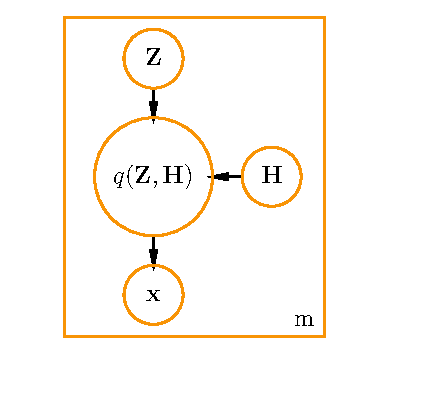
\includegraphics[width=0.25\textwidth]{./plots/notebooks/ae_plate.pdf}
\caption{Схема порождения вектора объектов $\mathbf{X}$, представленная в~\cite{vae_ard}.}
\label{fig:vae_ard}

\end{figure}

В данной работе предлагается метод последовательного порождения моделей глубокого обучения, основывающийся на применении вариационного вывода. Вариационный ввывод позволяет получить оценки правдоподобия модели с небольшими вычислительными затратами, а также проследить потенциальное начало переобучения модели без использования контрольной выборки. Для регуляризации структуры модели предлагается ввести априорное распределение на структуре, позволяющее проводить оптимизацию модели и ее структуры в различных режимах. В качестве метода оптимизации гиперпараметров выступают градиентные методы, что позволяет эффективно производить оптимизацию большого числа гиперпараметров, сопоставимого с числом параметров модели. 



\clearpage
\chapter{Выбор модели с использованием вариационного вывода}
В данной главе рассматривается задача выбора моделей глубокого обучения субоптимальной сложности. Под сложностью модели понимается правдоподобие модели~\eqref{eq:evidence}. Под субоптимальной сложностью понимается приближенная оценка правдоподобия модели, полученная с использованием вариационных методов. Вводятся вероятностные предположения о распределении параметров. На основе байесовского вывода предлагается функция правдоподобия модели. Для получения оценки правдоподобия применяются вариационные методы с использованием градиентных алгоритмов оптимизации. Проводится вычислительный эксперимент на нескольких выборках.

В данной работе предлагается метод получения вариационной нижней оценки  правдоподобия модели с использованием модифицированного алгоритма стохастического градиентного спуска. {Модификация заключается в добавлении шумовой компоненты. Эта компонента позволяет получить более точные оценки правдоподобия модели для сравнения моделей и выбора наиболее адекватной из них. } Рассматривается ряд модификаций базового алгоритма. {В качестве базового алгоритма выступает алгоритм оптимизации параметров модели с использованием стохастического градиентного спуска без контроля переобучения. Он заключается в итеративном вычислении градиента по параметрам от функции правдоподобия обучающей выборки и изменении значений параметров с его учетом.} Приводится сравнение с алгоритмом получения вариационной нижней оценки, представленном в~\cite{nips}. {Рассматриваются следующие модификации базового алгоритма:
%\begin{enumerate}
%\item 
оптимизация с кросс-валидацией с использованием и без использования регуляризации модели,
алгоритм получения вариационной оценки правдоподобия модели с применением нормального распределения,
алгоритм получения вариационной оценки правдоподобия с использованием стохастического градиентного спуска,
алгоритм получения вариационной оценки правдоподобия с использованием стохастической динамики Ланжевена.}
 { Данные алгоритмы решают следующие проблемы оптимизации моделей  градиентным спуском: оптимизация модели с меньшими затратами вычислительных ресурсов, быстрая сходимость оптимизации, контроль переобучения и выбор наиболее адекватной модели.
Под переобучением понимается потеря обобщающей способности модели с увеличением правдоподобия обучающей выборки~\cite{MacKay}. Переобучение характерно для моделей с большим количеством параметров, сопоставимым с мощностью обучающей выборки, что встречается в случае выбора моделей глубокого обучения~\cite{hinton_rbm, suts}.
}
Также алгоритмы имеют дальнейшую возможность применения к градиентным алгоритмам оптимизации гиперпараметров, описанным в~\cite{hyper}.

Свойства представленных в данной работе  алгоритмов исследуется на выборках, на которых проверялась работа алгоритма вероятностного обратного распространения ошибок~\cite{pbp}, где авторы акцентируются на оптимизации параметров модели. 


\section{Постановка задачи оптимизации правдоподобия моделей}
Определим понятие статистической сложности модели. Сложностью модели будем называть \textit{правдоподобие модели}~\eqref{eq:evidence}.
Пусть задано множество моделей $M$, для которых, возможно, не задан граф параметрического семейства моделей.
Для каждой модели $\mathbf{f} \in {M}$ заданы различные значения гиперпараметров $\mathbf{h}$. 
Рассмотрим два подхода к сравнению сложностей~\eqref{eq:evidence} моделей:
\begin{enumerate}
\item Модели $\mathbf{f}$ описываются общим параметрическим семействов моделей глубокого обучения $\mathfrak{F}$, т.е. имеют общий граф описания моделей $<V,E>$, общее пространство параметров $\mathbb{W}$ и пространство структур $\mathbb{\Gamma}$. При таком подходе сравнение сложности различных моделей является  адекватным, т.к. они определены на общем пространстве структур $\amsmathbb{\Gamma}$ и параметров $\mathbb{W}$. Возможно сравнение как статистической сложности модели, так и структурной.
\item Модели $\mathbf{f}$  не описываются общим параметрическим семействома. В данном случае однозначно определить структурную сложность модели нельзя (TODO: теорема?), поэтому будем полагать, что структуры модели определены однозначно, а априорнные распределения $p(\boldsymbol{\Gamma})$ структур моделей не учитываются при сравнении статистической сложности моделей.
\end{enumerate}
В данном разделе рассматривается второй вариант. Будем полгать, что структура модели $\boldsymbol{\Gamma}$ для вероятностной модели глубокого обучения $\mathbf{f}$ определена однозначно. 

\begin{defin} Сложностью модели $\mathbf{f}$ назовем правдоподобие модели:
\begin{equation}
\label{eq:model_evidence}
	p(\mathbf{y}|\mathbf{X},\mathbf{h}) = \int_{\mathbf{w} \in \mathbb{W}} p(\mathbf{y}|\mathbf{X},\mathbf{w}, \mathbf{h})p(\mathbf{w}|\mathbf{h})d\mathbf{w}.
\end{equation}
\end{defin}

Заметим, что основная часть данной главы также применим и в случае, когда модели описываются общим параметрическим семействов моделей глубокого обучения. В данном случае вместо интеграла~\eqref{eq:model_evidence} предлагается использовать интеграл~\eqref{eq:evidence}, учитывающий вероятностные предположения о структуре модели.


\begin{defin}Модель  $\mathbf{f}$ назовем оптимальной среди моделей $M$, если достигается максимум интеграла~\eqref{eq:model_evidence}.
\end{defin}


Требуется найти оптимальную модель $\mathbf{f}$ из заданного множества моделей $M$, а также значения ее параметров $\mathbf{w}$, доставляющие максимум апостериорной вероятности
\begin{equation}
\label{eq:var_inf_posterior}
	p(\mathbf{w}|\mathbf{y},\mathbf{X},\mathbf{h}) = \frac{p(\mathbf{y}|\mathbf{X}, \mathbf{w}, \mathbf{h})p(\mathbf{w}|\mathbf{h})}{p(\mathbf{y}|\mathbf{X}, \mathbf{h})}.
\end{equation}


%\begin{example_empty}
\begin{example}
Рассмотрим задачу линейной регрессии:
\[
	\mathbf{y} =\mathbf{X} \mathbf{w} + \boldsymbol{\varepsilon},\quad \boldsymbol{\varepsilon}  \sim \mathcal{N}(\mathbf{0},\mathbf{1}),\quad \mathbf{w} \sim  \mathcal{N}(\mathbf{0},\mathbf{A}^{-1}),
\]
где $\mathbf{A}$ --- диагональная матрица. 
Правдоподобие зависимой переменной имеет вид
\begin{equation}
\label{eq:example1}
	p(\mathbf{y}|  \mathbf{X}, \mathbf{w}, \mathbf{h}) = (2\pi) ^{-\frac{m}{2}} \textnormal{exp} \bigl(-\frac{1}{2}(\mathbf{y} -\mathbf{X} \mathbf{w})^\mathsf{T}(\mathbf{y} - \mathbf{X}\mathbf{w})\bigr),
\end{equation}
априорное распределение параметров модели имеет вид
\begin{equation}
\label{eq:prior}	
p(\mathbf{w}|\mathbf{h}) =  (2\pi) ^{-\frac{n}{2}} |\mathbf{A}|^{\frac{1}{2}} \textnormal{exp} (-\frac{1}{2}\mathbf{w}^\mathsf{T}\mathbf{A}\mathbf{w}).
\end{equation}

Правдоподобие модели~\eqref{eq:evidence} в этом примере вычисляется аналитически~\cite{hyperopt}:
\begin{equation}
\label{eq:ground}
	p(\mathbf{y}|\mathbf{X},\mathbf{h})  =  (2\pi) ^{-\frac{m}{2}} |\mathbf{A}|^{\frac{1}{2}} |\mathbf{H}|^{-\frac{1}{2}}  \textnormal{exp}\bigl(-\frac{1}{2}(\mathbf{y} -\mathbf{X} \hat{\mathbf{w}})^\mathsf{T}(\mathbf{y} - \mathbf{X}\hat{\mathbf{w}})\bigr)\textnormal{exp} \bigl(-\frac{1}{2}\hat{\mathbf{w}}^\mathsf{T}\mathbf{A}\hat{\mathbf{w}}\bigr),
\end{equation}
где $\hat{\mathbf{w}}$ --- значение наиболее вероятных~\eqref{eq:posterior} параметров модели:
\[
	\hat{\mathbf{w}} = \argmax p(\mathbf{w}|\mathbf{y}, \mathbf{X}, \mathbf{h}) = (\mathbf{A} + \mathbf{X}^\mathsf{T}\mathbf{X})^{-1}\mathbf{X}^\mathsf{T}\mathbf{y},
\]
$\mathbf{H}$ --- гессиан функции потерь $L$ модели:
\[
	\mathbf{H}	= \nabla \nabla_\mathbf{w} \left(\frac{1}{2} (\mathbf{y} -\mathbf{X} {\mathbf{w}})^\mathsf{T}(\mathbf{y} - \mathbf{X}{\mathbf{w}}) + \frac{1}{2}\mathbf{w}^\mathsf{T}\mathbf{A}\mathbf{w} \right) = \mathbf{A} + \mathbf{X}^\mathsf{T}\mathbf{X},
\]

\[ 
	L = - \textnormal{log} p(\mathbf{y}|  \mathbf{X}, \mathbf{w}, \mathbf{h}). 
\]
\end{example}

\begin{example}
Рассмотрим задачу классификации, в которой модель --- нейросеть с softmax-слоем на выходе:
\begin{equation}
\label{eq:softmax_example}
\mathbf{f} = \mathbf{f}_\textnormal{|V|}(\mathbf{f}_{|V|-1}(\dots \mathbf{f}_1(\mathbf{x}))),
\end{equation}
$\mathbf{f}_1, \dots, \mathbf{f}_{|V|}$ --- дифференцируемые функции, $\mathbf{f}_\textnormal{|V|}$ --- многомерная логистическая функция:
\begin{equation}
\label{eq:proba_softmax}
	\mathbf{f}_\textnormal{|V|} = \frac{\mathbf{f}_{|V|-1}(\dots \mathbf{f}_1(\mathbf{x}))}{\sum_{r=1}^Z \textnormal{exp}\bigl( {f}^{r}_{|V|-1}(\dots \mathbf{f}_1(\mathbf{x})) \bigr)},
\end{equation}
где ${f}_{|V|-1}^{r}$ --- $r$-я компонента функции $\mathbf{f}_{|V|-1}$. Компонента $r$ вектора $\mathbf{f}_{|V|}$ определяет вероятность принадлежности объекта $\mathbf{x}$ к классу $r$. Логарифм правдоподобия зависимой переменной аналогично~\eqref{eq:example1} имеет вид
\[
	\textnormal{log} p({y}|\mathbf{x}, \mathbf{w}, \mathbf{h}) =  \textnormal{log}~{f}^{y}_{|V|} (\mathbf{f}_{|V-1|}(\dots \mathbf{f}_1(\mathbf{x}))).
\]

Данная модель описывает многослойную сеть, аналогичную моделям семейства, представленного на Рис.~\ref{fig:scheme_mlp}.
\end{example}

Интеграл правдоподобия~\eqref{eq:model_evidence} модели является трудновычислимым для данного семейства моделей. Одним из методов вычисления приближенного значения правдоподобия является получение вариационной оценки правдоподобия.  


{В качестве функции, приближающей логарифм интеграла~\eqref{eq:model_evidence}, будем рассматривать его нижнюю оценку, полученную при помощи неравенства Йенсена~\cite{Bishop}. Получим нижнюю оценку логарифма правдоподобия модели, используя неравенство}
\begin{equation} 
\label{eq:var_elbo}
\textnormal{log}~p(\mathbf{y}|\mathbf{X},\mathbf{h})  = \int_{\mathbf{w}} q(\mathbf{w})\textnormal{log}~\frac{p(\mathbf{y},\mathbf{w}|\mathbf{X},\mathbf{h})}{q(\mathbf{w})}d\mathbf{w} + \textnormal{D}_\textnormal{KL}  \bigl(q(\mathbf{w})||p(\mathbf{w}|\mathbf{y}, \mathbf{X}, \mathbf{h})\bigr) \geq	
\end{equation} 
$$
\geq \int_{\mathbf{w}} q(\mathbf{w})\textnormal{log}~\frac{p(\mathbf{y},\mathbf{w}|\mathbf{X},\mathbf{h})}{q(\mathbf{w})}d\mathbf{w} =
$$

$$
= -\textnormal{D}_\textnormal{KL} \bigl(q(\mathbf{w})||p(\mathbf{w}|\mathbf{h})\bigr) + \int_{\mathbf{w}} q(\mathbf{w})\textnormal{log}~{p(\mathbf{y}|\mathbf{X},\mathbf{w},\mathbf{h})} d \mathbf{w},
$$
где $\textnormal{D}_\textnormal{KL}\bigl(q(\mathbf{w})||p(\mathbf{w} |\mathbf{h})\bigr)$ --- расстояние Кульбака--Лейблера между двумя распределениями: $$\textnormal{D}_\textnormal{KL}\bigl(q(\mathbf{w})||p(\mathbf{w} |\mathbf{h})\bigr) = -\int_{\mathbf{w}} q(\mathbf{w})\textnormal{log}~\frac{p(\mathbf{w} | \mathbf{h})}{q(\mathbf{w})}d\mathbf{w},$$
$$
p(\mathbf{y},\mathbf{w}|\mathbf{X},\mathbf{h}) = p(\mathbf{y}|\mathbf{X},\mathbf{h})p(\mathbf{w}|\mathbf{h}).
$$

{
\begin{defin} Вариационной оценкой логарифма правдоподобия модели~\eqref{eq:model_evidence} $\textnormal{log}~p(\mathbf{y}|\mathbf{X},\mathbf{h})$ называется оценка $\textnormal{log}~\hat{p}(\mathbf{y}|\mathbf{X},\mathbf{h})$, полученная аппроксимацией неизвестного апостериорного распределения $p(\mathbf{w}| \mathbf{y}, \mathbf{X}, \mathbf{h})$ заданным распределением $q(\mathbf{w})$.
\end{defin}
}


Будем рассматривать задачу нахождения вариационной оценки как задачу оптимизации. Пусть задано множество распределений $\mathfrak{Q} =\{q(\mathbf{w})\}$. Сведем задачу нахождения наиболее близкой вариационной нижней оценки интеграла~\eqref{eq:evidence} к оптимизации вида
\[
     \hat{q}(\mathbf{w}) = \argmax_{q \in \mathfrak{Q}}  \int_{\mathbf{w}} q(\mathbf{w})\textnormal{log}~\frac{p(\mathbf{y},\mathbf{w}|\mathbf{X},\mathbf{h})}{q(\mathbf{w})}d\mathbf{w}.
\]  
В данной работе в качестве множества $\mathfrak{Q}$ рассматривается нормальное распределение и распределение параметров, неявно получаемое оптимизацией градиентными методами. 

Оценка~\eqref{eq:var_elbo} является нижней, поэтому может давать некорректные оценки для правдоподобия~\eqref{eq:model_evidence}. Для того, чтобы оценить величину этой ошибки, докажем следующее утверждение.

\begin{theorem}[\cite{Bishop}]\label{st:st1} Пусть задано множество $\mathfrak{Q} = \{q(\mathbf{w})\}$ непрерывных распределений. Максимизация вариационной нижней оценки $$\int_{\mathbf{w}} q(\mathbf{w})\textnormal{log}~\frac{p(\mathbf{y},\mathbf{w}|\mathbf{X},\mathbf{h})}{q(\mathbf{w})}d\mathbf{w}$$  логарифма интеграла~\eqref{eq:evidence}  эквивалентна минимизации расстояния Кульбака--Лейблера между распределением $q(\mathbf{w}) \in \mathfrak{Q}$ и апостериорным распределением параметров $p(\mathbf{w}|\mathbf{y}, \mathbf{X}, \mathbf{h})$:
\begin{equation}
\label{eq:optim}
    \hat{q} = \argmax_{q \in Q} \int_{\mathbf{w}} q(\mathbf{w})\textnormal{log}~\frac{p(\mathbf{y},\mathbf{w}|\mathbf{X},\mathbf{h})}{q(\mathbf{w})}d\mathbf{w} \Leftrightarrow 	
    \hat{q} = \argmin_{q \in Q} \textnormal{D}_\textnormal{KL}  \bigl(q(\mathbf{w})||p(\mathbf{w}|\mathbf{y}, \mathbf{X}, \mathbf{h})\bigr),
\end{equation}

\[
	\textnormal{D}_\textnormal{KL}  \bigl(q(\mathbf{w})||p(\mathbf{w}|\mathbf{y}, \mathbf{X}, \mathbf{h})\bigr) =  \int_\mathbf{w} q(\mathbf{w}) \frac{q(\mathbf{w})}{p(\mathbf{w}|\mathbf{y}, \mathbf{X}, \mathbf{h})} d\mathbf{w}.
\]

\end{theorem}
\begin{proof}
Доказательство непосредственно следует из~\eqref{eq:var_elbo}. Вычитая из обеих частей равенства $\textnormal{D}_\textnormal{KL}  (q(\mathbf{w})||p(\mathbf{w}|\mathbf{y}, \mathbf{X}, \mathbf{h}))$, получим
\[
\textnormal{log}~p(\mathbf{y}|\mathbf{X},\mathbf{h}) - \textnormal{D}_\textnormal{KL}  (q(\mathbf{w})||p(\mathbf{w}|\mathbf{y}, \mathbf{X}, \mathbf{h}))  = \int_{\mathbf{w}} q(\mathbf{w})\textnormal{log}~\frac{p(\mathbf{y},\mathbf{w}|\mathbf{X},\mathbf{h})}{q(\mathbf{w})}d\mathbf{w},
\]
где $\textnormal{log}~p(\mathbf{y}|\mathbf{X},\mathbf{h})$ --- выражение, не зависящее от $q(\mathbf{w})$.
\end{proof}



Таким образом, задача нахождения вариационной оценки, близкой к значению интеграла~\eqref{eq:model_evidence} сводится к поиску распределения $\hat{q}$, аппроксимирующего распределение $p(\mathbf{w}|\mathbf{y}, \mathbf{X}, \mathbf{h})$ наилучшим образом. 

\begin{defin} Пусть задано множество распределений $\mathfrak{Q}$. Модель $\mathbf{f}$ назовем субоптимальной на множестве моделей $M$, если модель доставляет максимум нижней вариационной оценке интеграла~\eqref{eq:optim}
\begin{equation}
\label{eq:var_elbo2}
	\max_{q \in \mathfrak{Q}}\int_{\mathbf{w}} q(\mathbf{w})\textnormal{log}~\frac{p(\mathbf{y},\mathbf{w}|\mathbf{X},\mathbf{h})}{q(\mathbf{w})}d\mathbf{w}.
\end{equation}
\end{defin}

{
Субоптимальность модели может быть также названа вариационной оптимальностью модели или LB-оптимальностью (\textit{Lower Bound --- нижняя граница}) модели.}

Вариационная оценка~\eqref{eq:var_elbo} интерпретируется как оценка сложности модели по принципу минимальной длины описания~\eqref{eq:mdl}, где первое слагаемое определяет количество информации для описания выборки, а второе слагаемое --- длину описания самой модели~\cite{nips}.

В данной работе решается задача выбора субоптимальной модели при различных заданных множествах $\mathfrak{Q}$.

\section{Методы получения вариационной оценки правдоподобия}
Ниже представлены методы получения вариационных нижних оценок~\eqref{eq:var_elbo2} правдоподобия~\eqref{eq:evidence}. В первом параграфе рассматривается метод, основанный на аппроксимации апостериорного распределения $p( \mathbf{w}|\mathbf{y}, \mathbf{X}, \mathbf{h})$~\eqref{eq:posterior} многомерным гауссовым распределением с диагональной матрицей ковариаций. В последующих параграфах рассматриваются методы, основанные на различных модификациях стохастического градиентного спуска. 

\textbf{Аппроксимация нормальным распределением. }
В качестве множества $\mathfrak{Q} = \{q(\mathbf{w})\}$ задано параметрическое семейство нормальных распределений с диагональными матрицами ковариаций:
\begin{equation}
\label{eq:diag}
	q \sim \mathcal{N}(\boldsymbol{\mu}_q, \mathbf{A}^{-1}_q),\quad,\boldsymbol{\theta}=[\boldsymbol{\mu}_q, \textbf{diag}(\mathbf{A}^{-1}_q)]
\end{equation}
где $\mathbf{A}_q$ --- диагональная матрица ковариаций, $\boldsymbol{\mu}_q$ --- вектор средних компонент.

Пусть априорное распределение $p(\mathbf{w}|\mathbf{h})$~\eqref{eq:prior} параметров модели задано как нормальное:
\[
	p(\mathbf{w}|\mathbf{h}) \sim \mathcal{N}(\boldsymbol{\mu}, \mathbf{A}^{-1}),\quad \mathbf{h} = \textbf{diag}(\mathbf{A}^{-1}_q),
\] 
Тогда оптимизация~\eqref{eq:optim} имеет вид
\begin{equation}
\label{eq:norm_max}
 \int_{\mathbf{w}} q(\mathbf{w})\textnormal{log}~{p(\mathbf{y}|\mathbf{X},\mathbf{w},\mathbf{h})} d \mathbf{w} - D_\textnormal{KL}\bigl(q (\mathbf{w} )|| p (\mathbf{w}|\mathbf{h})\bigr) \to \max_{\mathbf{A}_q, \boldsymbol{\mu}_q},
\end{equation}
где расстояние $D_\textnormal{KL}$ между двумя гауссовыми величинами рассчитывается как 
\[
	D_\textnormal{KL}\bigl(q (\mathbf{w}) || p (\mathbf{w}|\mathbf{h})\bigr) = \frac{1}{2} \bigl( \textnormal{Tr} [\mathbf{A}\mathbf{A}^{-1}_q] + (\boldsymbol{\mu} - \boldsymbol{\mu}_q)^\mathsf{T}\mathbf{A}(\boldsymbol{\mu} - \boldsymbol{\mu}_q) - u +\textnormal{ln}~|\mathbf{A}^{-1}| - \textnormal{ln}~|\mathbf{A}_q^{-1}| \bigr).
\]
В качестве приближенного значения интеграла $$\int_{\mathbf{w}} q(\mathbf{w})\textnormal{log}~{p(\mathbf{y}|\mathbf{X},\mathbf{w},\mathbf{h})} d \mathbf{w}$$ предлагается использовать формулу
\[
\int_{\mathbf{w}} q(\mathbf{w})\textnormal{log}~{p(\mathbf{y}|\mathbf{X},\mathbf{w},\mathbf{h})} d \mathbf{w} \approx \sum_{i=1}^m \textnormal{log}~p({y}_i|\mathbf{x}_i, \mathbf{w}_i),
\]
где $\mathbf{w}_i$  --- реализация случайной величины из распределения $q(\mathbf{w})$.

Итоговая функция оптимизации~\eqref{eq:norm_max} имеет вид
\begin{equation}
\label{eq:gaus}
	\mathbf{f} = \argmax_{\mathbf{A}_q, \boldsymbol{\mu}_q} \sum_{i=1}^m \textnormal{log}~p({y}_i|\mathbf{x}_i, \mathbf{w}_i) - D_\textnormal{KL}\bigl(q (\mathbf{w} )|| p (\mathbf{w}|\mathbf{h})\bigr) =
\end{equation}
\[
   = \argmin_{\boldsymbol{\theta}} L( \boldsymbol{\theta}| \mathbf{h}, \mathbf{X}, \mathbf{y}).
\]

%\begin{example_empty} 
%\hspace{\parindent}
\begin{example}
Пусть  задана выборка $\mathfrak{D}$, в которой переменная ${y}$ не зависит от $\mathbf{x}$:
\begin{equation}
\label{eq:example_post}
	{y} \sim \mathcal{N}(\mathbf{w}, \mathbf{B}^{-1}),
\end{equation}

\[
	\mathbf{B}^{-1} = \left( \begin{array}{cc}
	2 & 1,8 \\
	1,8 & 2\\
	\end{array}  \right),
\]
\[
	p(\mathbf{w}|\mathbf{h}) = \mathcal{N}(\mathbf{0}, \mathbf{I}).
\]

График аппроксимации распределения параметров представлен на рис.~\ref{fig:var},\textit{а}. Как видно из графика, с использованием метода~\eqref{eq:gaus} получено грубое приближение апостериорного распределения $p(\mathbf{w}|\mathbf{y}, \mathbf{X}, \mathbf{h})$, что может существенно занизить оценку правдоподобия модели.


\begin{figure}[tbh!]



\minipage{0.32\textwidth}
 \caption*{\textit{а}}
  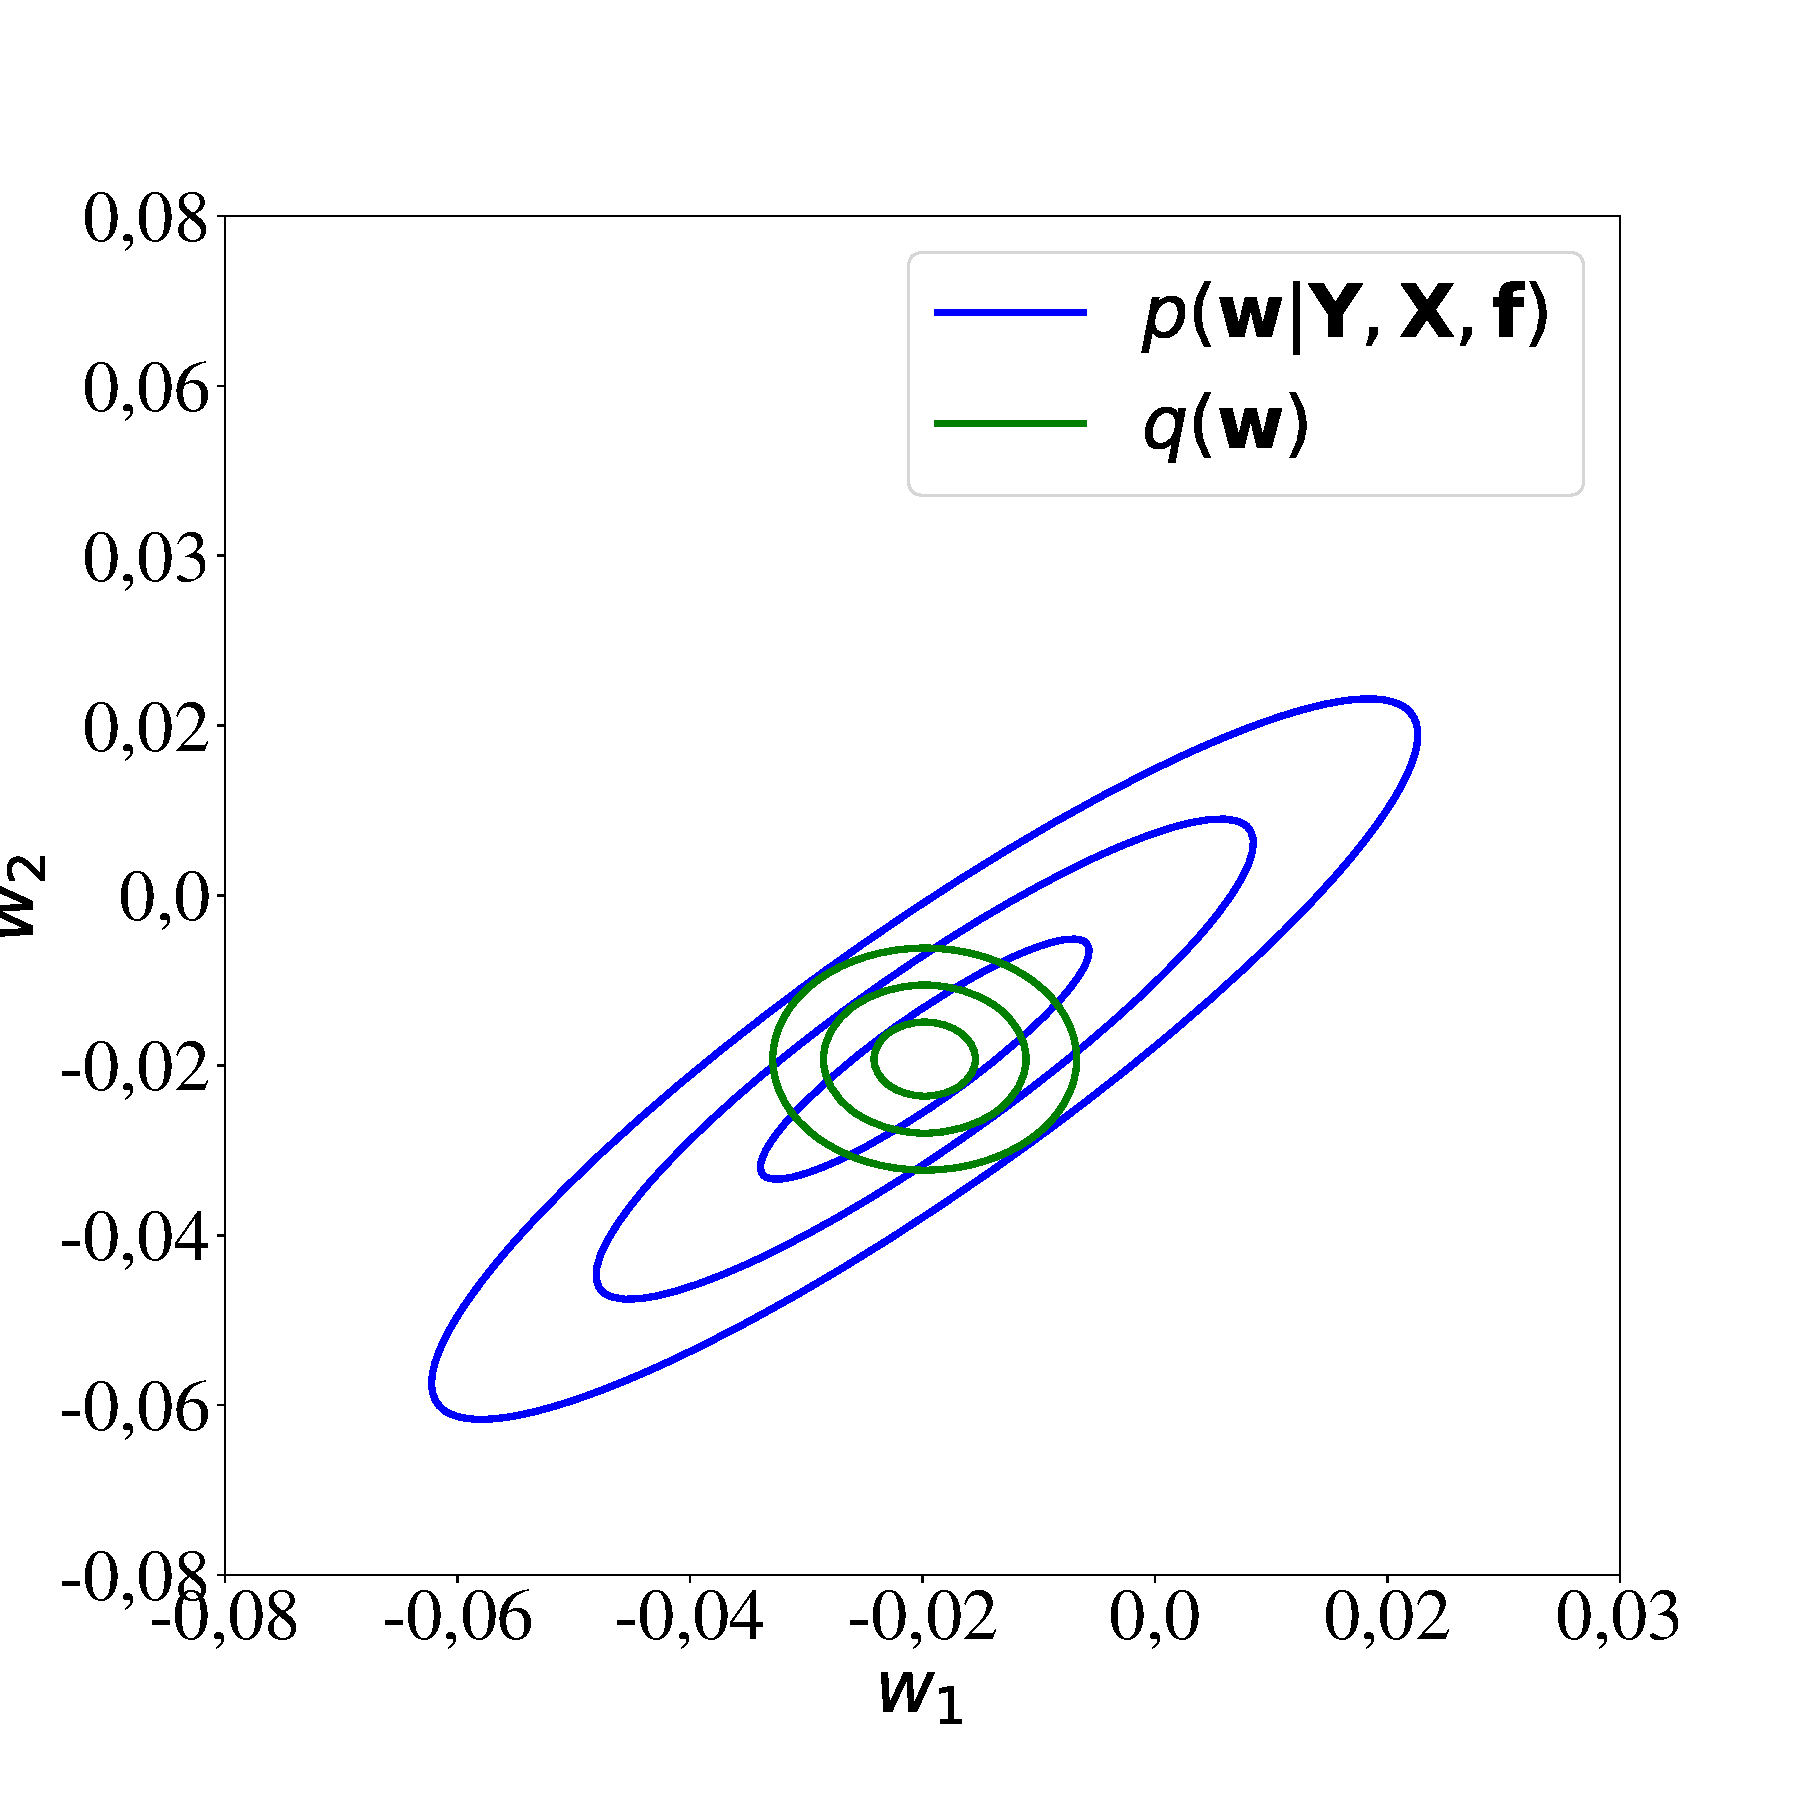
\includegraphics[width=\linewidth]{./plots/var/mf.pdf}

\endminipage\hfill
\minipage{0.32\textwidth}
\caption*{\textit{б}}
 
  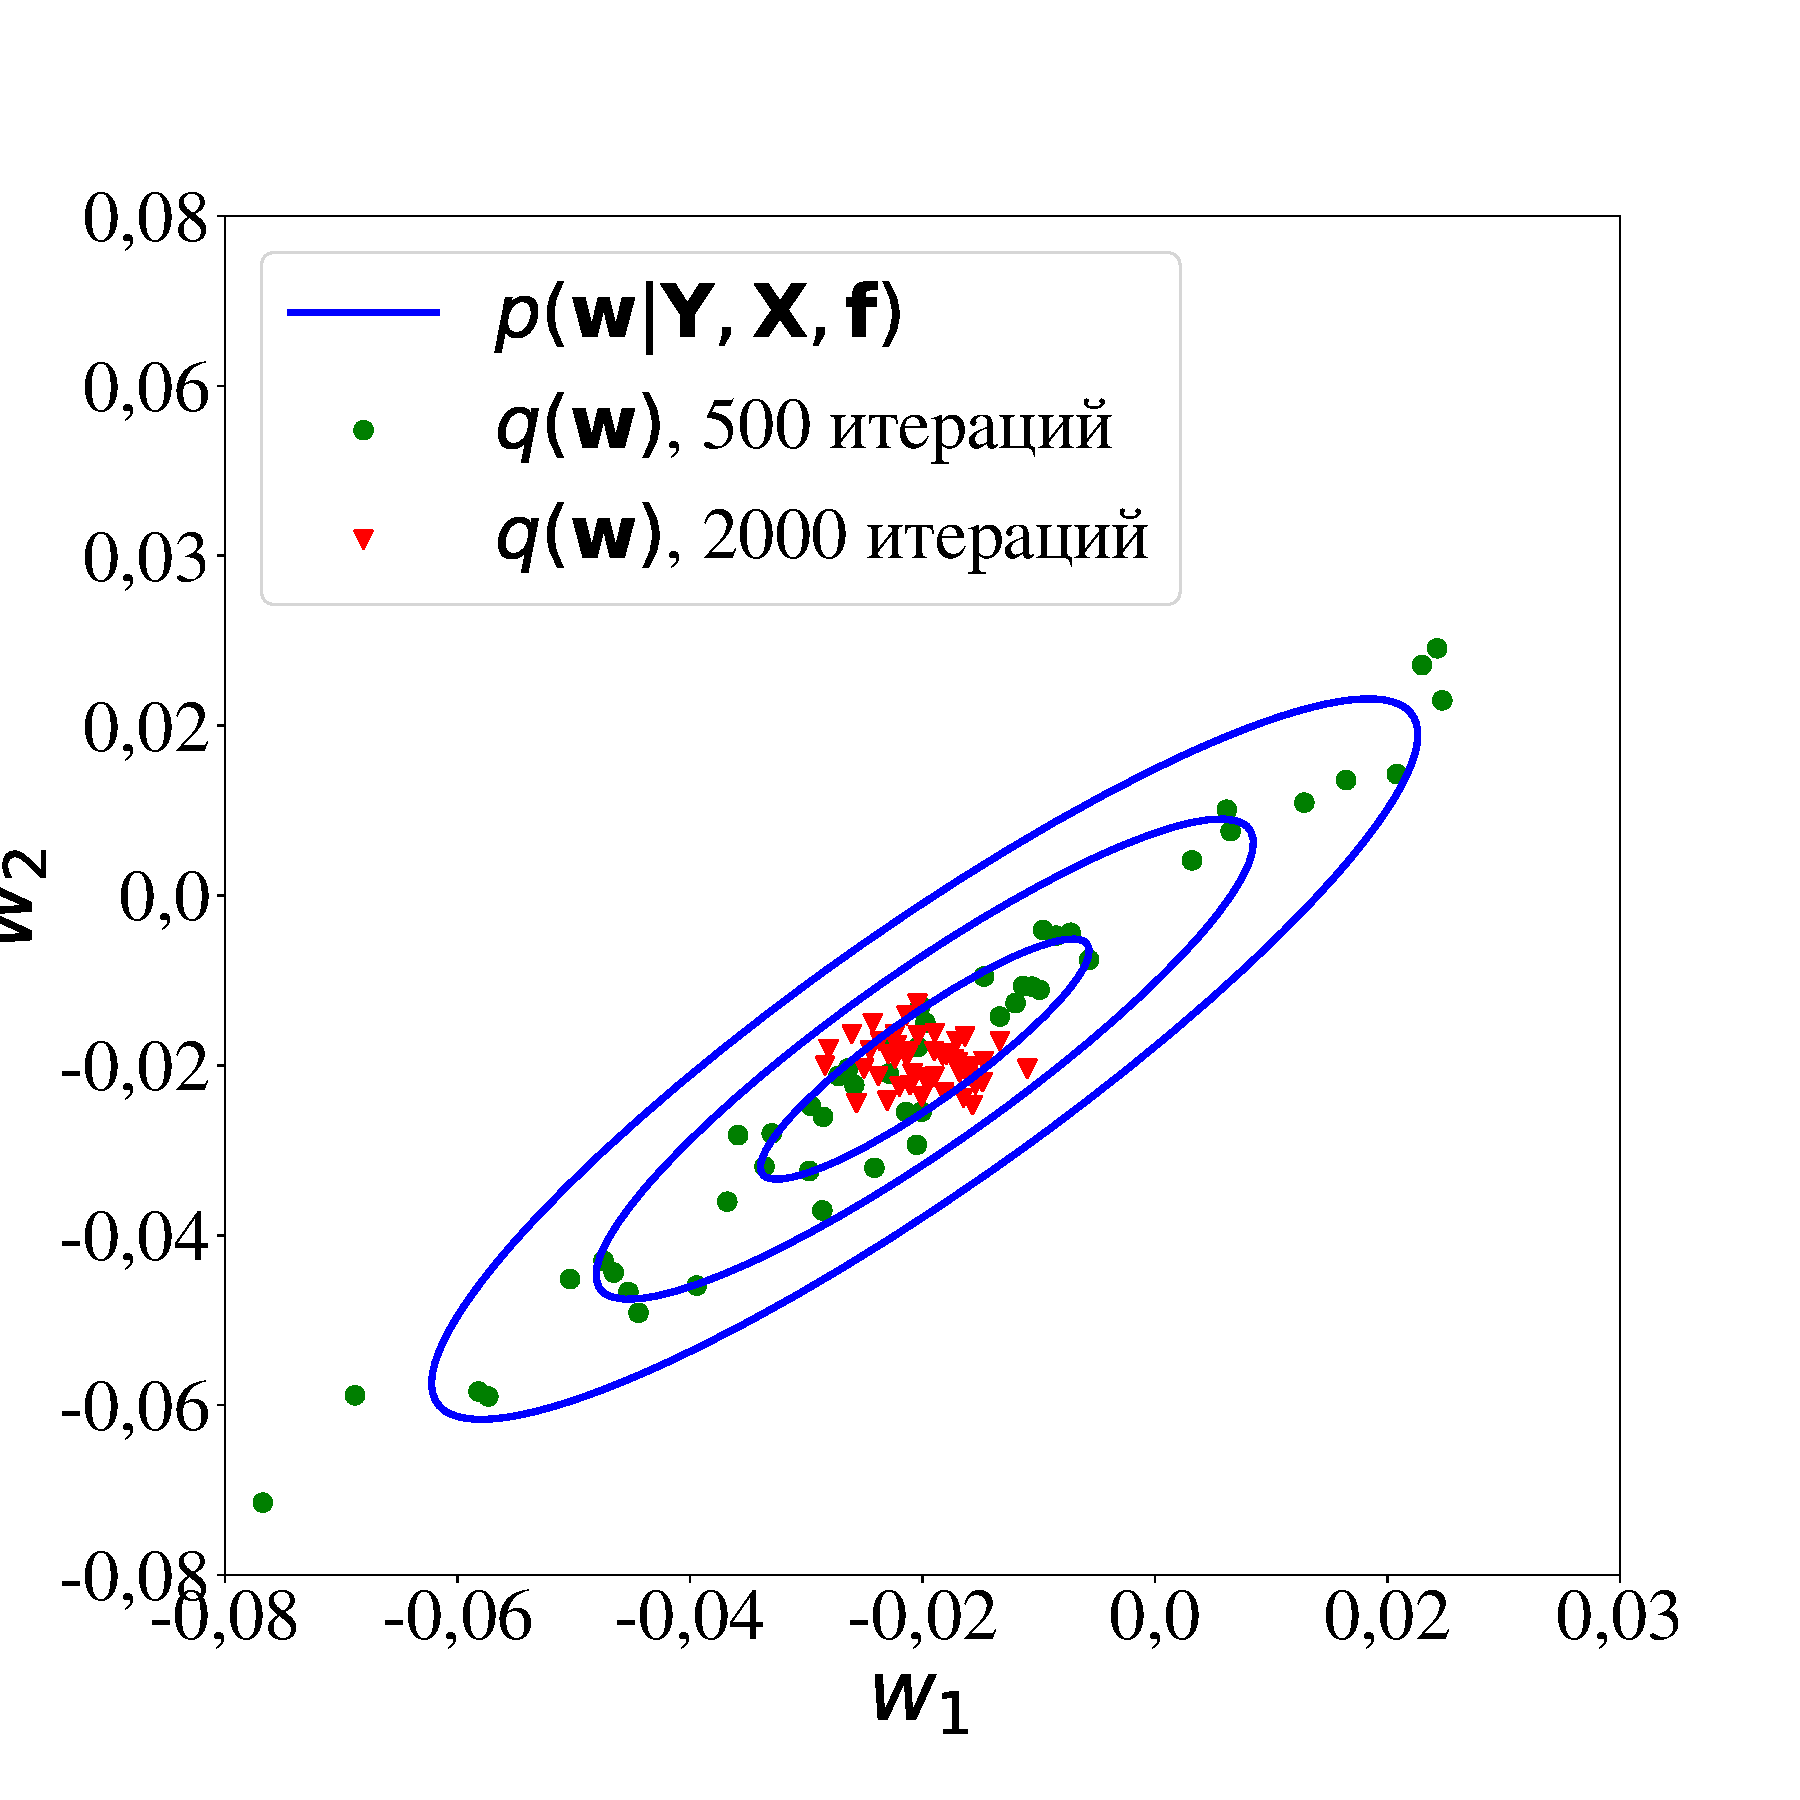
\includegraphics[width=\linewidth]{./plots/var/sgd.pdf}
 \endminipage\hfill
\minipage{0.32\textwidth}%
 \caption*{\textit{в}}

  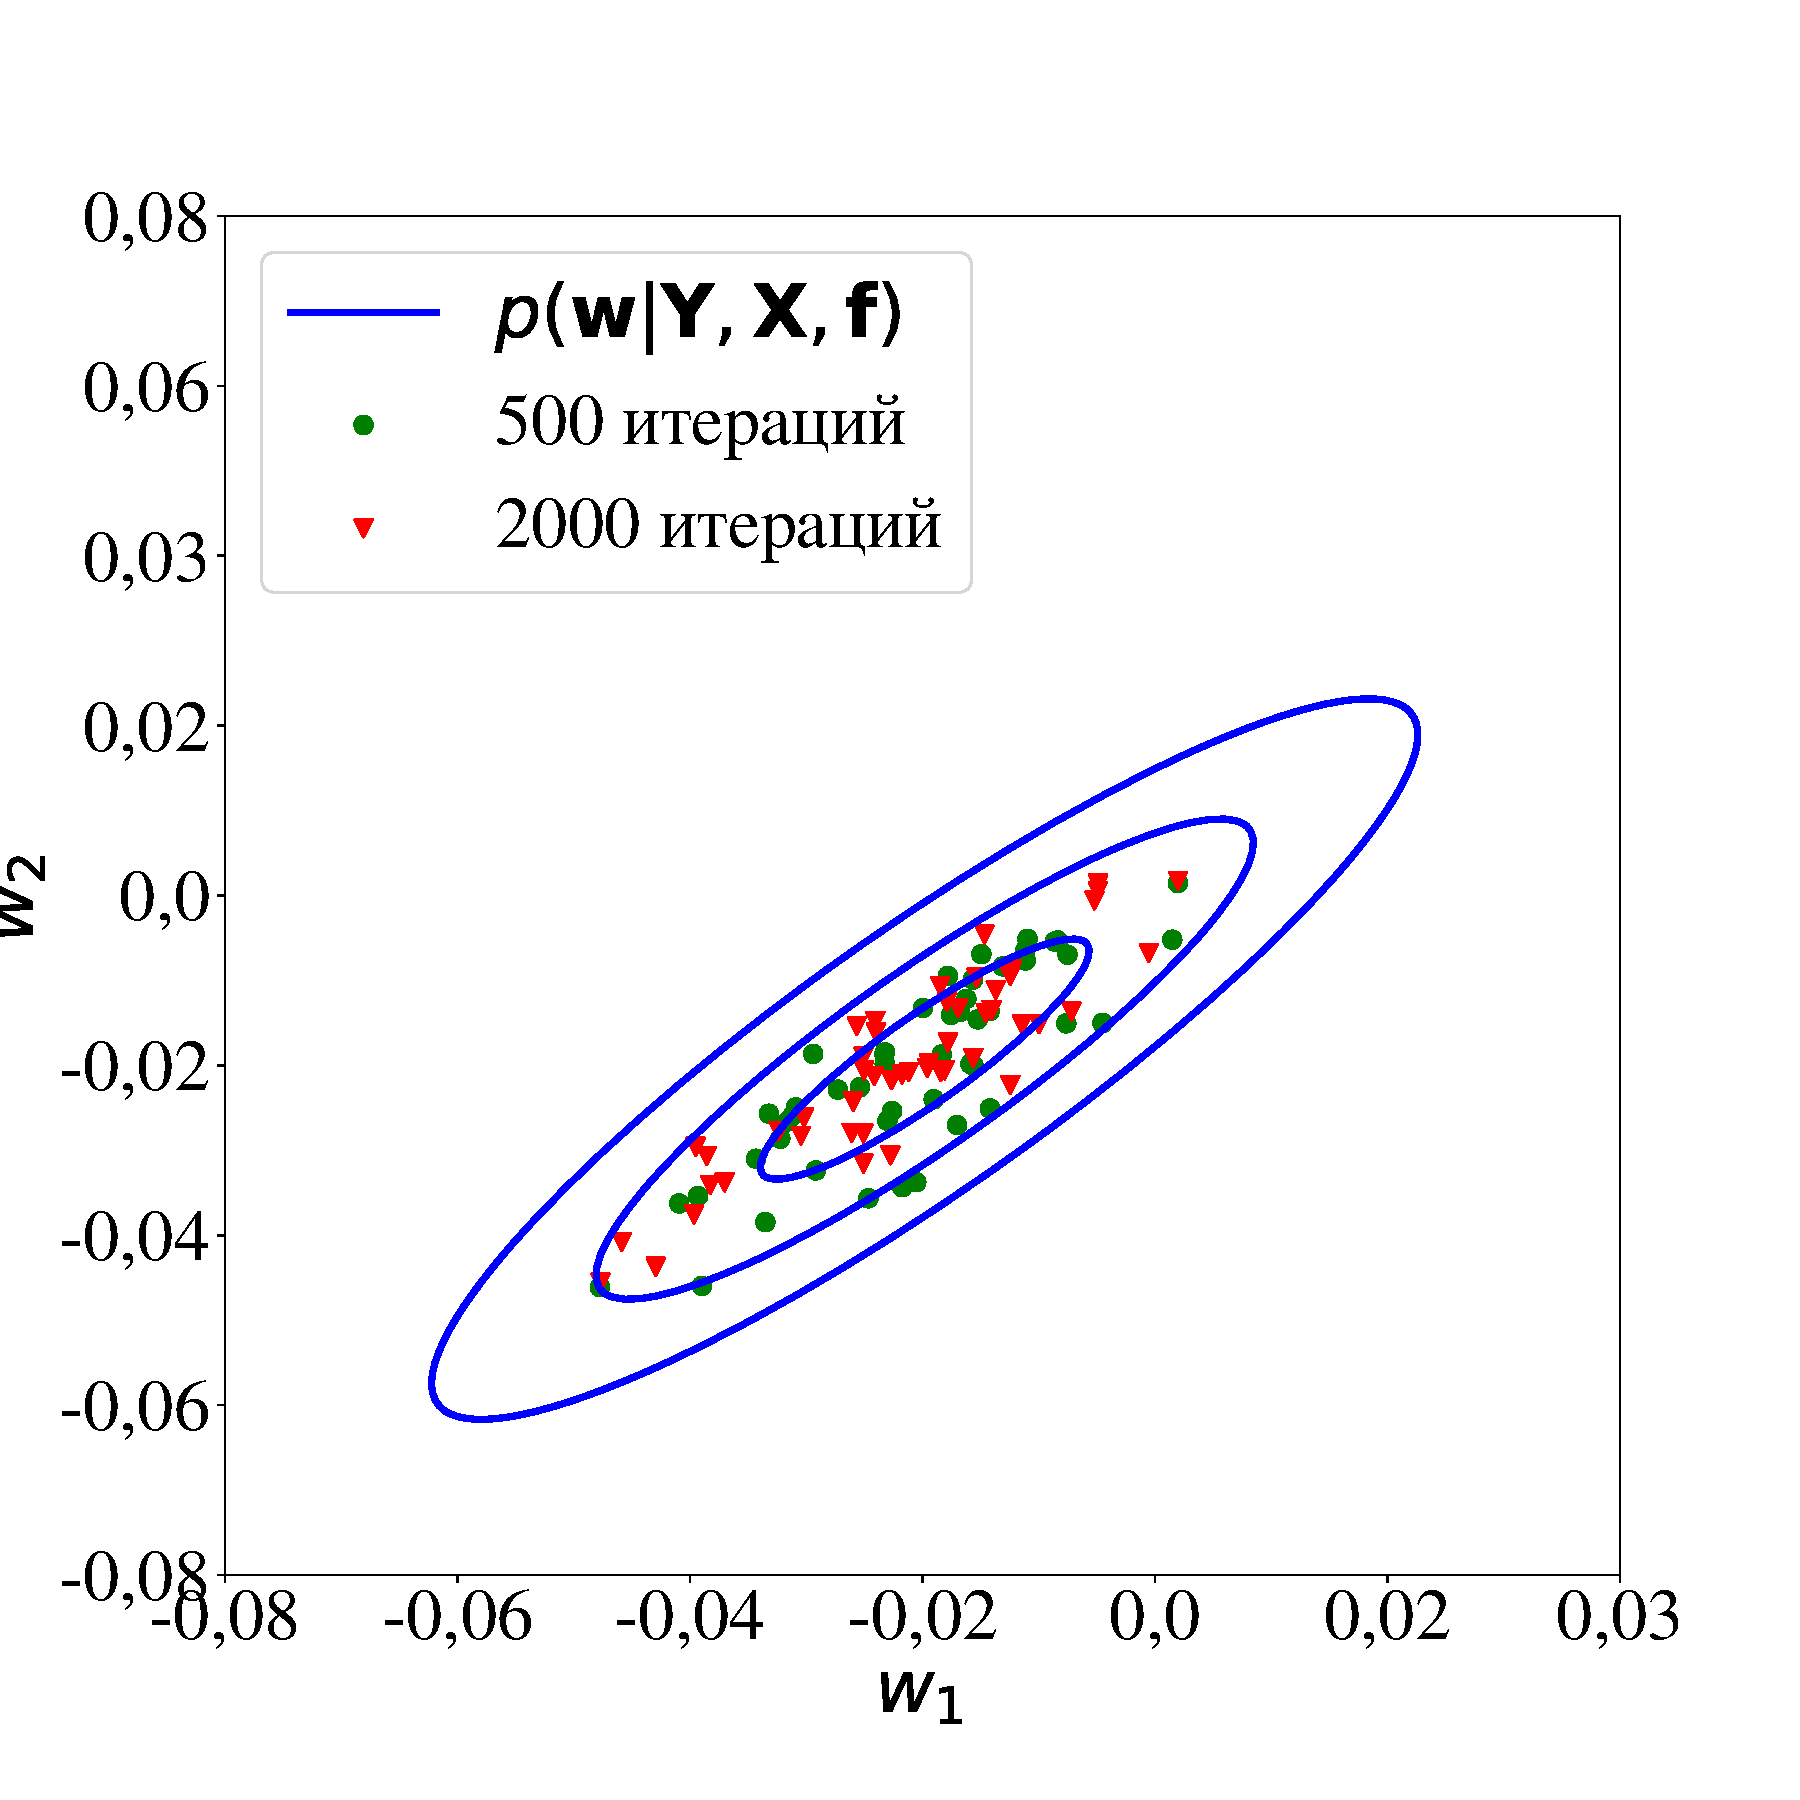
\includegraphics[width=\linewidth]{./plots/var/lang.pdf}
\endminipage\hfill
  \caption{Аппроксимация распределения \textit{а}) нормальным распределением, \textit{б}) распределением,
полученным с помощью градиентного спуска, \textit{в}) с использованием стохастической динамики Ланжевена.}
\label{fig:var}
\end{figure}




{Данный пример показывает, что качество итоговой аппроксимации распределения $p(\mathbf{w}|\mathbf{y}, \mathbf{X}, \mathbf{h})$ значительно зависит от схожести распределений $\hat{q}$ и $p(\mathbf{w}|\mathbf{y}, \mathbf{X}, \mathbf{h})$. В силу диагональности матрицы $\mathbf{A}_q$ и полного ранга матрицы $\mathbf{B}$  итоговое распределение $\hat{q}$ не может адекватно приблизить данное распределение  $p(\mathbf{w}|\mathbf{y}, \mathbf{X}, \mathbf{h})$.}

\end{example}

%\end{example_empty}
\textbf{Аппроксимация с использованием градиентного метода. }
В качестве множества распределений $\mathfrak{Q} = \{q(\mathbf{w})\}$, аппроксимирующих неизвестное распределение $\textnormal{log}~p(\mathbf{y}|\mathbf{X},\mathbf{h})$, используются распределения параметров, полученные в ходе их оптимизации.

Представим неравенство~\eqref{eq:var_elbo}
\begin{equation}
\label{eq:var_elbo_entropy}
 \textnormal{log}~p(\mathbf{y}|\mathbf{X},\mathbf{h}) \geq \int_\mathbf{w} q(\mathbf{w})\textnormal{log}~\frac{p(\mathbf{y},\mathbf{w}|\mathbf{X}, \mathbf{h})}{q(\mathbf{w})}d\mathbf{w} =  \mathsf{E}_{q(\mathbf{w)}}\bigl(\textnormal{log~}p (\mathbf{y}, \mathbf{w}|\mathbf{X}, \mathbf{h})\bigr) - \mathsf{S}\bigl({q(\mathbf{w)}}\bigr),
\end{equation}
где $\mathsf{S}$ --- энтропия распределения:
\[
\mathsf{S}\bigl({q(\mathbf{w)}}\bigr) = - \int_{\mathbf{w}} q(\mathbf{w})\textnormal{log}~q(\mathbf{w})d\mathbf{w},
\]
$$p (\mathbf{y}, \mathbf{w}|\mathbf{X}, \mathbf{h}) = p (\mathbf{w}| \mathbf{h}) p (\mathbf{y}|\mathbf{X}, \mathbf{w}, \mathbf{h}),$$
$\mathsf{E}_{q(\mathbf{w)}}\bigl(\textnormal{log~}p (\mathbf{y}, \mathbf{w}|\mathbf{X}, \mathbf{h})\bigr)$ --- матожидание логарифма вероятности $\textnormal{log~}p (\mathbf{y}, \mathbf{w}|\mathbf{X}, \mathbf{h})$:
\[
	\mathsf{E}_{q(\mathbf{w)}}\bigl(\textnormal{log~}p (\mathbf{y}, \mathbf{w}|\mathbf{X}, \mathbf{h})\bigr) = \int_\mathbf{w} \textnormal{log~}p (\mathbf{y}, \mathbf{w}|\mathbf{X}, \mathbf{h}) q(\mathbf{w}) d\mathbf{w}.
\]

Оценка распределений производится при оптимизации параметров. Оптимизация выполняется в режиме мультистарта~\cite{multi}, т.е. при запуске оптимизации параметров модели из нескольких разных начальных приближений. Основная проблема такого подхода~---~вычисление энтропии $\mathsf{S}$ распределений $q(\mathbf{w}) \in Q$. Ниже представлен метод получения оценок энтропии~\eqref{eq:entropy} ~$\mathsf{S}$ и оценок правдоподобия~\eqref{eq:var_elbo_entropy}.

Запустим $r$ процедур оптимизаций модели $\mathbf{f}$ из разных начальных приближений:
\[
	L( \boldsymbol{\theta}| \mathbf{h}, \mathbf{X}, \mathbf{y}) = -\sum_{l=1}^r \text{log}p(\mathbf{y}, \mathbf{w}^l|\mathbf{X}, \mathbf{h})  \to \min, \quad \boldsymbol{\theta} = [\mathbf{w}^1, \dots, \mathbf{w}^r],
\] 
где $r$ --- число оптимизаций,
\begin{equation}
\label{eq:loss_func}
\text{log}p(\mathbf{y}, \mathbf{w}^l|\mathbf{X}, \mathbf{h}) = -\sum_{i=1}^m \textnormal{log}p({y}_i, \mathbf{w}^l |\mathbf{x}_i, \mathbf{h}) = -\textnormal{log}~p(\mathbf{w}^l|\mathbf{h}) - \sum_{i=1}^m \textnormal{log}p({y}_i |\mathbf{x}_i, \mathbf{w}^l, \mathbf{h}).
\end{equation}

Пусть начальные приближения параметров $\mathbf{w}^1, \dots, \mathbf{w}^r$ порождены из некоторого начального распределения $q^0(\mathbf{w})$:
\[ 
	\mathbf{w}^1, \dots, \mathbf{w}^r \sim q^0(\mathbf{w}). 
\]


%Обозначим за  $\mathbf{w}^l, g \in \{1,\dots,r\}$ значения параметров $\mathbf{w}^1, \dots, \mathbf{w}^r$ на  текущем шаге оптимизации. 


Для дальнейшего описания метода введем понятие оператора градиентного спуска, являющегося частным случаем оператора оптимизации~\eqref{eq:optim_operator}.
\begin{defin}
Оператором градиентного спуска назовем оператор оптимизации вида
\begin{equation}
\label{eq:sgd}
	T( \boldsymbol{\theta}| L,\mathbf{X},  \mathbf{y},  \mathbf{h}, {\beta_{\text{lr}}}) = \boldsymbol{\theta} - \beta_{\text{lr}} \nabla L( \boldsymbol{\theta}| \mathbf{h}, \mathbf{X}, \mathbf{y}), 
\end{equation}
где  $\beta_{\text{lr}}$ --- длина шага градиентного спуска.
\end{defin}

Пусть значения $\mathbf{w}^1, \dots, \mathbf{w}^r$  --- реализации случайной величины из некоторого распределения $q(\mathbf{w})$. Начальная энтропия распределения $q(\mathbf{w})$ соответствует энтропии распределения $q^0(\mathbf{w})$, из которого были порождены начальные приближения оптимизации параметров $\mathbf{w}^1, \dots, \mathbf{w}^r$. Под действием оператора $T$ распределение параметров $\mathbf{w}_1, \dots, \mathbf{w}_r$ изменяется. Для учета энтропии распределений, полученных в ходе оптимизации,
{ формализуем метод,  представленный в~\cite{early}. }

\begin{theorem}~Пусть $T$ --- оператор градиентного спуска,
 $L$ --- функция потерь, градиент $\nabla L$ которой имеет константу Липшица $C_L$.  Пусть $\mathbf{w}^1,\dots,\mathbf{w}^r$ ---  начальные приближения оптимизации модели, где $r$ --- число начальных приближений. Пусть $\beta_{\text{lr}}$ --- длина шага градиентного спуска, такая что
\begin{equation}
\label{eq:ineq}
\beta_{\text{lr}}<\frac{1}{C_L}, \quad \beta_{\text{lr}} < \bigl(\max_{l \in \{1,\dots,r\}}\lambda_\textnormal{max} (\mathbf{H}(\mathbf{w}^l))\bigr)^{-1}, 
\end{equation}
где $\lambda_\textnormal{max}$ --- наибольшее по модулю собственное значение гессиана  $\mathbf{H}$ функции потерь $L$.

При выполнении неравенств~\eqref{eq:ineq} разность энтропий распределений $q'(\mathbf{w}), q(\mathbf{w})$ на смежных шагах почти наверное сходится к следующему выражению: 
\begin{equation}
\label{eq:entropy}
	\mathsf{S}\bigl(q'(\mathbf{w})) -  \mathsf{S}\bigl(q(\mathbf{w}))  \approx  \frac{1}{r}\sum_{l=1}^r \bigl(-\beta_{\text{lr}} \textnormal{Tr}[\mathbf{H}(\mathbf{w}'^l)] - \beta_{\text{lr}} \textnormal{Tr}[\mathbf{H}(\mathbf{w}'^l)\mathbf{H}(\mathbf{w}'^l)]  \bigr) + o_{\beta_{\text{lr}}^2 \to 0}(1),
\end{equation}
где $\mathbf{H}$ --- гессиан функции потерь $L$.
\end{theorem}

Предварительно приведем две леммы, требуемые для доказательства теоремы.
\begin{lemma}[~\cite{sgd_conv}] Пусть $T$ --- оператор градиентного спуска, $L$ --- дважды дифференцируемая функция потерь, градиент $\nabla L$ которой имеет константу Липшица $C_L$.  Пусть для длины шага $\beta_{\text{lr}}$ выполнено неравенство 
$
	\beta_{\text{lr}}<\frac{1}{C_L}.
$
Тогда $T$ является диффеоморфизмом.
\end{lemma}

\begin{lemma}[~\cite{entropy}] Пусть $\mathbf{w}$ --- случайный вектор с непрерывным распределением $q(\mathbf{w})$. Пусть $T$ --- биективное отображение вектора $\mathbf{w}$ в пространство той же размерности. Пусть $q'(\mathbf{w})$ --- распределение вектора $T(\mathbf{w})$. Тогда справедливо утверждение
\begin{equation}
\label{eq:entropy_biject}
	\mathsf{S}\bigl(q'(\mathbf{w})\bigr) -  \mathsf{S}\bigl(q(\mathbf{w})\bigr)  = \int_\mathbf{w}  q'(\mathbf{w}) \textnormal{log}~\left|\frac{\partial{T(\mathbf{w})}}{\partial{\mathbf{w}}}\right| d\mathbf{w}.
\end{equation}
\end{lemma}


\begin{proof}




Рассмотрим очередной шаг оптимизации. При $\beta_{\text{lr}}<\frac{1}{C}$ оператор градиентного спуска $T$ является диффеоморфизмом, а значит, и биекцией, справедлива формула~\eqref{eq:entropy_biject}.
По усиленному закону больших чисел 
\[
	\mathsf{S}\bigl(q'(\mathbf{w})\bigr) -  \mathsf{S}\bigl(q(\mathbf{w})\bigr)  \approx  \frac{1}{r}\sum_{l=1}^r \textnormal{log}~\left|\frac{\partial{T(\mathbf{w}'^l)}}{\partial{\mathbf{w}}}\right|,
\]
где знак $\approx$ означает сходимость почти наверное.
Логарифм якобиана  $\textnormal{log}~\left|\frac{\partial{T(\mathbf{w}'^l)}}{\partial{\mathbf{w}}}\right|$ оператора $T$ запишем как%~\cite{early}:
\begin{equation}
\label{eq:to_taylor}
	\textnormal{log}~\left|\frac{\partial{T(\mathbf{w}'^l)}}{\partial{\mathbf{w}}}\right| = \textnormal{log}~|\mathbf{I} - \beta_{\text{lr}}\mathbf{H}| = \sum_{i=1}^{|\mathbb{W}|} \textnormal{log}~(1-\beta_{\text{lr}}\lambda_i),
\end{equation}
где $\lambda_i$ --- $i$-е собственное значение гессиана $\mathbf{H}$.

При $(\beta_{\text{lr}}\lambda_i) ^ 2 \leq (\beta_{\text{lr}}\lambda_\textnormal{max})^2 < 1$ выражение~\eqref{eq:to_taylor} раскладывается в ряд Тейлора:
\[
	 \sum_{t=1}^{|\mathbb{W}|} \textnormal{log}~(1-\beta_{\text{lr}}\lambda_i) =  -\beta_{\text{lr}} \textnormal{Tr}[\mathbf{H}(\mathbf{w}'^l)] - \beta_{\text{lr}}^2 \textnormal{Tr}[\mathbf{H}(\mathbf{w}'^l)\mathbf{H}(\mathbf{w}'^l)] + o_{\beta_{\text{lr}}^2 \to 0}(1).
\]
Просуммировав полученные выражения для каждой точки мультистарта и вынеся $o_{\beta_{\text{lr}}^2 \to 0}(1)$ за скобки, получим выражение~\eqref{eq:entropy}, что и требовалось доказать.

\end{proof} 	


Получим итоговую формулу для оценки правдоподобия модели.
\begin{theorem}\label{st:st2}
Оценка~\eqref{eq:var_elbo_entropy} на шаге оптимизации $\tau$ представима в виде
\begin{equation}
\label{eq:ev_grad_full}
\textnormal{log}~\hat{p}(\mathbf{y}|\mathbf{X}, \mathbf{h}) \approx \frac{1}{r} \sum_{g = 1}^r L(\mathbf{w}^l_\tau| \mathbf{X}, \mathbf{y})  + 
\end{equation}
\[
+\mathsf{S}\big(q^0(\mathbf{w})\bigr) + \frac{1}{r}\sum_{b=1}^\tau\sum_{l=1}^r \bigl(-\beta_{\text{lr}} \textnormal{Tr}[\mathbf{H}(\mathbf{w}_b^l)] - \beta_{\text{lr}}^2 \textnormal{Tr}[\mathbf{H}(\mathbf{w}_b^l)\mathbf{H}(\mathbf{w}_b^l)]  \bigr) 
\]
с точностью до слагаемых вида $o_{\beta_{\text{lr}}^2 \to 0}(1)$,
где $\mathbf{w}_b^l$ --- $l$-я реализация параметров модели на шаге оптимизации $b$, $q^0(\mathbf{w})$ --- начальное распределение.
\end{theorem}



\begin{proof} Представим энтропию распределения $q^\tau(\mathbf{w})$ следующим образом:
\[
\mathsf{S}\bigl(q^\tau(\mathbf{w})\bigr) = \mathsf{S}\bigl(q^0(\mathbf{w})\bigr) - \mathsf{S}\bigl(q^0(\mathbf{w})\bigr) + \mathsf{S}\bigl(q^1(\mathbf{w})\bigr) - \mathsf{S}\bigl(q^1(\mathbf{w})\bigr) +\dots -
\mathsf{S}\bigl(q^{\tau-1}(\mathbf{w})\bigr) + \mathsf{S}\bigl(q^\tau(\mathbf{w})\bigr).
\]
Каждая разность энтропий вида $\mathsf{S}\bigl(q^b(\mathbf{w})\bigr) - \mathsf{S}\bigl(q^{b-1}(\mathbf{w})\bigr)$ по теореме с точностью до $o_{\beta_{\text{lr}}^2 \to 0}(1)$ представима в виде
\begin{equation}
\label{eq:eq_sums}
	\mathsf{S}\bigl(q^b(\mathbf{w})\bigr) -  \mathsf{S}\bigl(q^{b-1}(\mathbf{w})\bigr)  \approx  \frac{1}{r}\sum_{l=1}^r \bigl(-\beta_{\text{lr}} \textnormal{Tr}[\mathbf{H}(\mathbf{w}_b^l)] - \beta_{\text{lr}}^2 \textnormal{Tr}[\mathbf{H}(\mathbf{w}_b^l)\mathbf{H}(\mathbf{w}_b^l)]  \bigr).
\end{equation}

Формула~\eqref{eq:ev_grad_full} получается подстановкой в выражение~\eqref{eq:var_elbo_entropy} суммы выражений вида~\eqref{eq:eq_sums}, а также начальной энтропии $\mathsf{S}\bigl(q^0(\mathbf{w}))$.
\end{proof}

В~\cite{early} предлагается алгоритм приближенного вычисления для выражения, находящегося под знаком суммы в~\eqref{eq:ev_grad_full}:
\[
	-\beta_{\text{lr}} \textnormal{Tr}[\mathbf{H}(\mathbf{w}^l)] - \beta_{\text{lr}}^2 \textnormal{Tr}[\mathbf{H}(\mathbf{w}^l)\mathbf{H}(\mathbf{w}^l)]  \approx \mathbf{r}_0^\mathsf{T}\bigl(-2\mathbf{r}_0 + 3\mathbf{r}_1 -\mathbf{r}_2\bigr),
\]
где вектор $\mathbf{r}_0$  порождается из нормального распределения:
$$\mathbf{r}_0 \sim \mathcal{N}(\mathbf{0}, \mathbf{I}), \quad \mathbf{r}_1 = \mathbf{r}_0 - \beta_{\text{lr}} \mathbf{r}_0^\mathsf{T} \nabla \nabla L, \quad \mathbf{r}_2 = \mathbf{r}_1 - \beta_{\text{lr}} \mathbf{r}_1^\mathsf{T} \nabla \nabla L.$$


Заметим, что при приближении параметров модели к точке экстремума оценка правдоподобия устремляется в минус бесконечность в силу постоянно убывающей энтропии. Таким образом, чем ближе градиентный метод приближает параметры модели к точке экстремума, тем менее точной становится оценка правдоподобия модели. Один из методов борьбы с данной проблемой представлен в следующих параграфах.
\begin{figure}
\begin{algorithmic}[1]
\REQUIRE $\mathbf{X}, \mathbf{y}, p(\mathbf{w}|\mathbf{h})$;
\REQUIRE критерий останова $\text{Stop}$, начальное распределение параметров $q^0$, количество точек мультистарта $r$, функция потерь $L$, ее первая и вторая производные;
\ENSURE $\textnormal{log}~\hat{p}(\mathbf{y}|\mathbf{X}, \mathbf{h})$;
\FOR{$l=1,\dots,r$}
\STATE $\mathbf{w}^l \sim q^0$;
\ENDFOR
\STATE $\mathsf{S} = \mathsf{S}\bigl(q^0)$;
\WHILE{не достигнут критерий останова $\text{Stop}$}
\STATE $\boldsymbol{\theta} = T( \boldsymbol{\theta}| L,\mathbf{X},  \mathbf{y},  \mathbf{h}, {\beta_{\text{lr}}});$
\FOR{$l=1,\dots,r$}
\STATE $\mathbf{r}_0 \sim \mathcal{N}(\mathbf{0}, \mathbf{I})$;
\STATE $\mathbf{r}_1 = \mathbf{r}_0 - \beta_{\text{lr}} \mathbf{r}^{\mathsf{T}}_0 \nabla \nabla L(\mathbf{w}^l| \mathbf{y}, \mathbf{X})$;
\STATE $\mathbf{r}_2 = \mathbf{r}_1 - \beta_{\text{lr}} \mathbf{r}^{\mathsf{T}}_1 \nabla \nabla L(\mathbf{w}^l| \mathbf{y}, \mathbf{X})$;
\STATE $\mathsf{S}^l = \mathbf{r}_0^\mathsf{T}\bigl(-2\mathbf{r}_0 + 3\mathbf{r}_1 -\mathbf{r}_2\bigr)$;
\ENDFOR
\STATE $\mathsf{S} = \frac{1}{r}\sum_{l=1}^r \mathsf{S}^l$;
\ENDWHILE
\STATE $\hat{p}(\mathbf{y}|\mathbf{X}, \mathbf{w}, \mathbf{h}) = \frac{1}{r}\sum_{l=1}^r p(\mathbf{y}|\mathbf{X}, \mathbf{w}^l, \mathbf{h})$;
\STATE $\hat{p}(\mathbf{w} | \mathbf{h}) = \frac{1}{r}\sum_{l=1}^r p(\mathbf{w}^l| \mathbf{h})$;
\STATE $\textnormal{log}~\hat{p}(\mathbf{y}|\mathbf{X}, \mathbf{h}) = \textnormal{log}~\hat{p}(\mathbf{y}|\mathbf{X}, \mathbf{w}, \mathbf{h}) +\textnormal{log}~\hat{p}(\mathbf{w} | \mathbf{h})$;
	
\end{algorithmic}
\caption{Псевдокод алгоритма получения вариационной нижней оценки правдоподобия модели с использованием градиентного спуска}
\label{fig:algo}

\end{figure}



\textbf{Модификация алгоритма оптимизации модели.} \\
В качестве оператора $T$ предлагается использовать псевдослучайный стохастический градиентный спуск, т.е. градиентный спуск~\eqref{eq:sgd_operator}, оптимизирующий параметры $\mathbf{w}^1,\dots,\mathbf{w}^r$ по некоторой случайной подвыборке $\hat{\mathbf{X}}, \hat{\mathbf{y}}$, одинаковой для каждой точки старта $\mathbf{w}^1,\dots,\mathbf{w}^r$:
\[
    T( \boldsymbol{\theta}| L,\mathbf{X},  \mathbf{y},  \mathbf{h}, {\beta_{\text{lr}}}) = \boldsymbol{\theta} - \beta_{\text{lr}}\nabla L(\boldsymbol{\theta}|   \mathbf{h},  \hat{\mathbf{X}}, \hat{\mathbf{y}}),
\]
где $\beta{\text{lr}}$ --- шаг градиентного спуска, $\hat{\mathbf{y}}, \hat{\mathbf{X}}$ --- случайная подвыборка заданной мощности выборки $\mathfrak{D}$.
где $\hat{\mathbf{X}}$ --- случайная подвыборка выборки ${\mathbf{X}}$, одинаковая для всех точек мультистарта, $\hat{\mathbf{y}}$ --- соответствующие метки классов, $$|\hat{\mathbf{X}}| = \hat{m}.$$

Как и версия алгоритма с использованием градиентного спуска~\eqref{eq:sgd}, основной проблемой модифицированного алгоритма оценки интеграла~\eqref{eq:var_elbo2} является грубость аппроксимации исходного распределения $p(\mathbf{w}|\mathbf{f},\mathfrak{D})$.

Рассмотрим пример~\eqref{eq:example_post}.
График аппроксимации распределения $p(\mathbf{w}|\mathbf{y}, \mathbf{X}, \mathbf{h})$ представлен на рис.~\ref{fig:var},\textit{б}.
Как видно из графика, градиентный спуск сходится к моде распределения. При небольшом количестве итераций полученное распределение также слабо аппроксимирует апостериорное распределение. {При приближении к точке экстремума снижается вариационная оценка правдоподобия модели, что  интерпретируется как возможное начало переобучения~\cite{early}. Таким образом, снижение оценки~\eqref{eq:ev_grad_full} можно использовать как критерий остановки оптимизации модели для снижения эффекта переобучения.  }

На рис.~\ref{fig:var} представлена  {аппроксимация распределения $p(\mathbf{w}|\mathbf{Y}, \mathbf{X}, \mathbf{h})$ различными методами: \textit{а}) нормальным распределением с диагональной матрицей ковариаций, \textit{б}) с помощью градиентного спуска, \textit{в}) с помощью стохастической динамики Ланжевена. Точками отмечены параметры модели $\mathbf{f}$, полученные в ходе нескольких запусков оптимизации и являющиеся реализациями случайной величины с распределением $q(\mathbf{w})$. Нормальное распределение слабо аппроксимирует распределение $p(\mathbf{w}|\mathbf{Y}, \mathbf{X}, \mathbf{h})$ в силу диагональности матрицы ковариаций. Распределение, полученное с помощью градиентного спуска, слабо аппроксимирует распределение $p(\mathbf{w}|\mathbf{Y}, \mathbf{X}, \mathbf{h})$, так как сходится к моде.}





\textbf{Аппроксимация с использованием динамики Ланжевена}\\
Для достижения нижней оценки интеграла~\eqref{eq:var_elbo2}, более близкой к реальному значению логарифма интеграла~\eqref{eq:evidence}, чем оценка с использованием градиентного спуска, предлагается использовать стохастическую динамику Ланжевена~\cite{langevin}. Стохастическая динамика Ланжевена представляет собой вариант стохастического градиентного спуска с добавлением гауссового шума:
\begin{equation}
\label{eq:langevin}
	T( \boldsymbol{\theta}| L,\mathbf{X},  \mathbf{y},  \mathbf{h}, {\beta_{\text{lr}}}) = \boldsymbol{\theta} -\frac{m}{\hat{m}}  \beta_{\text{lr}} \nabla L(\boldsymbol{\theta}| \mathbf{h}, \hat{\mathbf{X}}, \hat{\mathbf{y}})  + \boldsymbol{\varepsilon}, \quad  \boldsymbol{\varepsilon} \sim \mathcal{N}(\mathbf{0}, {\frac{\beta_{\text{lr}}}{2}}\mathbf{I}),
\end{equation}
где $\hat{\mathbf{X}}$ --- псевдослучайная подвыборка, $\hat{\mathbf{y}}$ --- соответствующие метки, $\hat{m}$ --- размер подвыборки. Длина шага оптимизации $\beta_{\text{lr}}$ удовлетворяет  {условиям, гарантирующим сходимость алгоритма в стандартных ситуациях~\cite{langevin}}:
\[
	\sum_{\tau=1}^\infty \beta_{\text{lr}}^\tau = \infty, \quad \sum_{\tau=1}^\infty (\beta_{\text{lr}}^\tau)^2 < \infty.
\]

Для оценки энтропии с учетом шума $\boldsymbol{\varepsilon}$ предлагается использовать следующее неравенство~\cite{entropy,var_grad}:
\[
\hat{\mathsf{S}}\bigl(q^\tau(\mathbf{w})\bigr)   \geq \frac{1}{2}|\mathbb{W}|\textnormal{log}\left(\textnormal{exp}\left(\frac{2\mathsf{S}\bigl(q^\tau(\mathbf{w})\bigr)}{|\mathbb{W}|}\right) + \textnormal{exp}\left(\frac{2\mathsf{S}\bigl( \boldsymbol{\varepsilon})}{|\mathbb{W}|}\right)\right),
\]
{где  $\tau$ --- текущий шаг оптимизации,} $\mathsf{S}\bigl( \mathcal{N}({0}, {\frac{\beta_{\text{lr}}}{2}})\bigr)$ --- энтропия нормального распределения, $\hat{\mathsf{S}}(q^\tau(\mathbf{w}))$ --- энтропия распределения $q^\tau$ с учетом добавленного шума~$\boldsymbol{\varepsilon}$.


В отличие от стохастического градиентного спуска стохастическая динамика Ланжевена сходится к апостериорному распределению параметров $p(\mathbf{w}|\mathfrak{D},\mathbf{h})$~\cite{langevin, langevin_sato}.  График аппроксимации апостериорного распределения с использованием динамики Ланжевена представлен на рис.~\ref{fig:var},\textit{в}. При одинаковом количестве итераций динамика Ланжевена продолжает аппроксимировать апостериорное распределение, в то время как градиентный спуск сходится к моде распределения. {Как видно из графика, алгоритм, основанный на стохастической динамике Ланжевена, способен давать более точную вариационную оценку правдоподобия~\eqref{eq:var_elbo2}. В то же время алгоритм более требователен к настройке параметров оптимизации~\cite{sgld}: \textit{``быстро изменяющаяся кривизна [траекторий параметров модели] делает методы стохастической градиентной динамики Ланжевена по умолчанию неэффективными''.}}
%However, the rapidly changing curvature renders default SGLD methods inefficient




\section{Анализ методов выбора моделей}
Для анализа свойств предложенного критерия субоптимальности в задачах регрессии и классификации, а также методов получения нижних оценок правдоподобия модели в задачах выбора моделей был проведен ряд вычислительных экспериментов на выборках Boston Housing, Protein Structure, а также на небольшой подвыборке YearPredictionMSD (далее --- Boston, Protein и MSD)~\cite{UCI} {и подвыборке изображений рукописных цифр MNIST~\cite{mnist}}.

{Для выборок Boston, Protein и MSD} была рассмотрена задача регрессии
\[
	\mathbf{y} = \mathbf{f}(\mathbf{X}, \mathbf{w}) + \boldsymbol{\varepsilon}, \quad  \boldsymbol{\varepsilon} \sim \mathcal{N}(\mathbf{0}, \mathbf{I}), \mathbf{f} \in {M}.
\]

В качестве множества моделей $M$ были рассмотрены  нейросети с одним скрытым слоем и softplus-функцией активации:
\begin{equation}
\label{eq:model}
	\mathbf{f}(\mathbf{w}, \mathbf{X}) =   \textbf{softplus}\bigl(\mathbf{X} \mathbf{w}_0^{0,1} \bigr)  \mathbf{w}_0^{1,2},
\end{equation}
где $\mathbf{w}_0^{0,1}  \in \mathbb{R}^{n\times n_1}$ --- матрица параметров скрытого слоя нейросети, $\mathbf{w}_0^{1,2} \in \mathbb{R}^{n_1\times 1}$ --- матрица параметров выходного слоя нейросети, {$\textbf{softplus}(\mathbf{X}) = \textbf{log}\bigl(1+\textbf{exp}(\mathbf{X})\bigr)$}.

{Для выборки Boston также было рассмотрено множество моделей с тремя скрытыми слоями, построенных аналогично однослойной модели~\eqref{eq:model}. Размер каждого слоя равнялся 50.}

{Для выборки MNIST была рассмотрена задача бинарной классификации: из выборки были взяты только объекты, соответствующие цифрам 7 и 9. Размерность выборки была понижена с 784 до 50 методом главных компонент аналогично~\cite{firefly}. Для анализа моделей, полученных в случае высокой вероятности переобучения, из обучающей выборки были взяты первые 500 объектов. В качестве модели рассматривалась нейросеть с тремя скрытыми слоями}
\[
    \mathbf{f}(\mathbf{w}, \mathbf{X}) =   \boldsymbol{\sigma}(\textbf{softplus}\bigl(  \textbf{softplus} \bigl(\textbf{softplus}\bigl(\mathbf{X} \mathbf{w}_0^{0,1} \bigr)  \mathbf{w}_0^{1,2} \bigr) \mathbf{w}_0^{2,3} \bigr) \mathbf{w}_0^{3,4}),
\]
{где $\boldsymbol{\sigma}(\mathbf{X}) = \bigl(1+\textbf{exp}(\mathbf{-X})\bigr)^{-1}$  --- сигмоида, $\mathbf{W}_0^{0,1}, \dots, \mathbf{w}_0^{3,4}$ --- параметры нейросети.}



Во всех экспериментах исходная выборка $\mathfrak{D}$ разбивалась на обучающую и контрольную подвыборки:
$
	\mathfrak{D} = \mathfrak{D}_\textnormal{train} \sqcup \mathfrak{D}_\textnormal{text}.
$

Оптимизация параметров производилась на подвыборке $\mathfrak{D}_\textnormal{train}$. Для контроля переобучения некоторых алгоритмов из обучающей выборки $\mathfrak{D}_\textnormal{train}$ формировалась валидационная выборка $\mathfrak{D}_\textnormal{valid}$, на которой не проводилась оптимизация параметров  модели. Мощность валидационной выборки $\mathfrak{D}_\textnormal{valid}$ составляла 0,1 мощности обучающей выборки  $\mathfrak{D}_\textnormal{train}$, объекты для валидационной выборки выбирались случайным образом независимо для каждого старта алгоритма.
Качество полученных моделей проверялось на подвыборке $\mathfrak{D}_\textnormal{test}.$ Критерием качества модели выступали среднеквадратичное отклонение вектора $\mathbf{y}$ от вектора $\mathbf{f}(\mathbf{w}, \mathbf{X})$ (RMSE) {в случае задачи регрессии и доля верно предсказанных меток класса (Accuracy) в задаче классификации}, а также { соответствующие критерии } при возмущении элементов выборки:
\begin{equation}
\label{eq:rmse}
	\textnormal{RMSE}_{\sigma} =\textnormal{RMSE}\bigl(\mathbf{f}( \mathbf{w}, \mathbf{X}+\boldsymbol{\varepsilon}), \mathbf{y}\bigr),  \quad \boldsymbol{\varepsilon} \sim \mathcal{N}(\mathbf{0}, \sigma \mathbf{I}).
\end{equation}

Были рассмотрены шесть алгоритмов.
\begin{enumerate}
\item Базовый алгоритм: оптимизация параметров без валидации и ранней остановки. Оптимизация проводилась с использованием стохастического градиентного спуска~\eqref{eq:sgd}. Для данного алгоритма априорное распределение $p(\mathbf{w}|\mathbf{h})$ не использовалось.
\item Алгоритм с валидацией. Для контроля переобучения во время оптимизации качество модели оценивалось на валидационной выборке $\mathfrak{D}_\textnormal{valid}$. Для данного алгоритма априорное распределение также не использовалось.
\item Алгоритм с валидацией и введенным априорным распределением. В качестве априорного распределения рассматривается распределение вида
$
	\mathbf{w} \sim \mathcal{N}(\mathbf{0}, \alpha \mathbf{I}), 
$
где $\alpha$ --- дисперсия.

\item Нахождение вариационной нижней оценки с использованием стохастического градиентного спуска.
\item Нахождение вариационной нижней оценки с использованием стохастической динамики Ланжевена.
\item Нахождение вариационной нижней оценки с аппроксимацией нормальным распределением ~\eqref{eq:gaus}.
\end{enumerate}




Параметры модели выбирались из точек мультистарта (алгоритмы 1---5) или порождались из распределения $\hat{q}$ (алгоритм 6). Количество точек мультистарта: $r=10$ {для задач регрессии и $r=25$ для задачи классификации}.
Для алгоритмов 2---6 применялась ранняя остановка: каждые $\tau_\textnormal{val}$ итераций производилась оценка внутреннего критерия качества модели. В качестве критерия остановки применялось следующее условие: значение внутреннего критерия качества не улучшалось $3\tau_\textnormal{val}$ итераций. Для разных алгоритмов внутренним критерием качества выступали различные величины:
\begin{enumerate}[1)]
\item функция потерь $L$~\eqref{eq:loss_func} на валидационной выборке $\mathfrak{D}_\textnormal{valid}$ для алгоритмов $2,3$;
\item вариационная нижняя оценка правдоподобия~\eqref{eq:var_elbo} на обучающей выборке $\mathfrak{D}_\textnormal{train}$ для алгоритмов $4,5,6$.
\end{enumerate}

Для каждой модели назначались различные значения параметра $\alpha (\alpha \in \{10, \dots, 10^9\})$ и длины шага оптимизации $\beta_{\text{lr}}$, отбирались наилучшие модели. 



Описание эксперимента представлено в табл.~1. Результаты экспериментов представлены в табл.~2. На рис.~\ref{fig:noise_in_data} представлен график зависимости $\textnormal{RMSE}_{\sigma}$ от параметра~$\sigma$~{ для однослойных моделей}. 

\begin{figure}[tbh!]


\minipage{0.32\textwidth}
\caption*{\textit{а}}
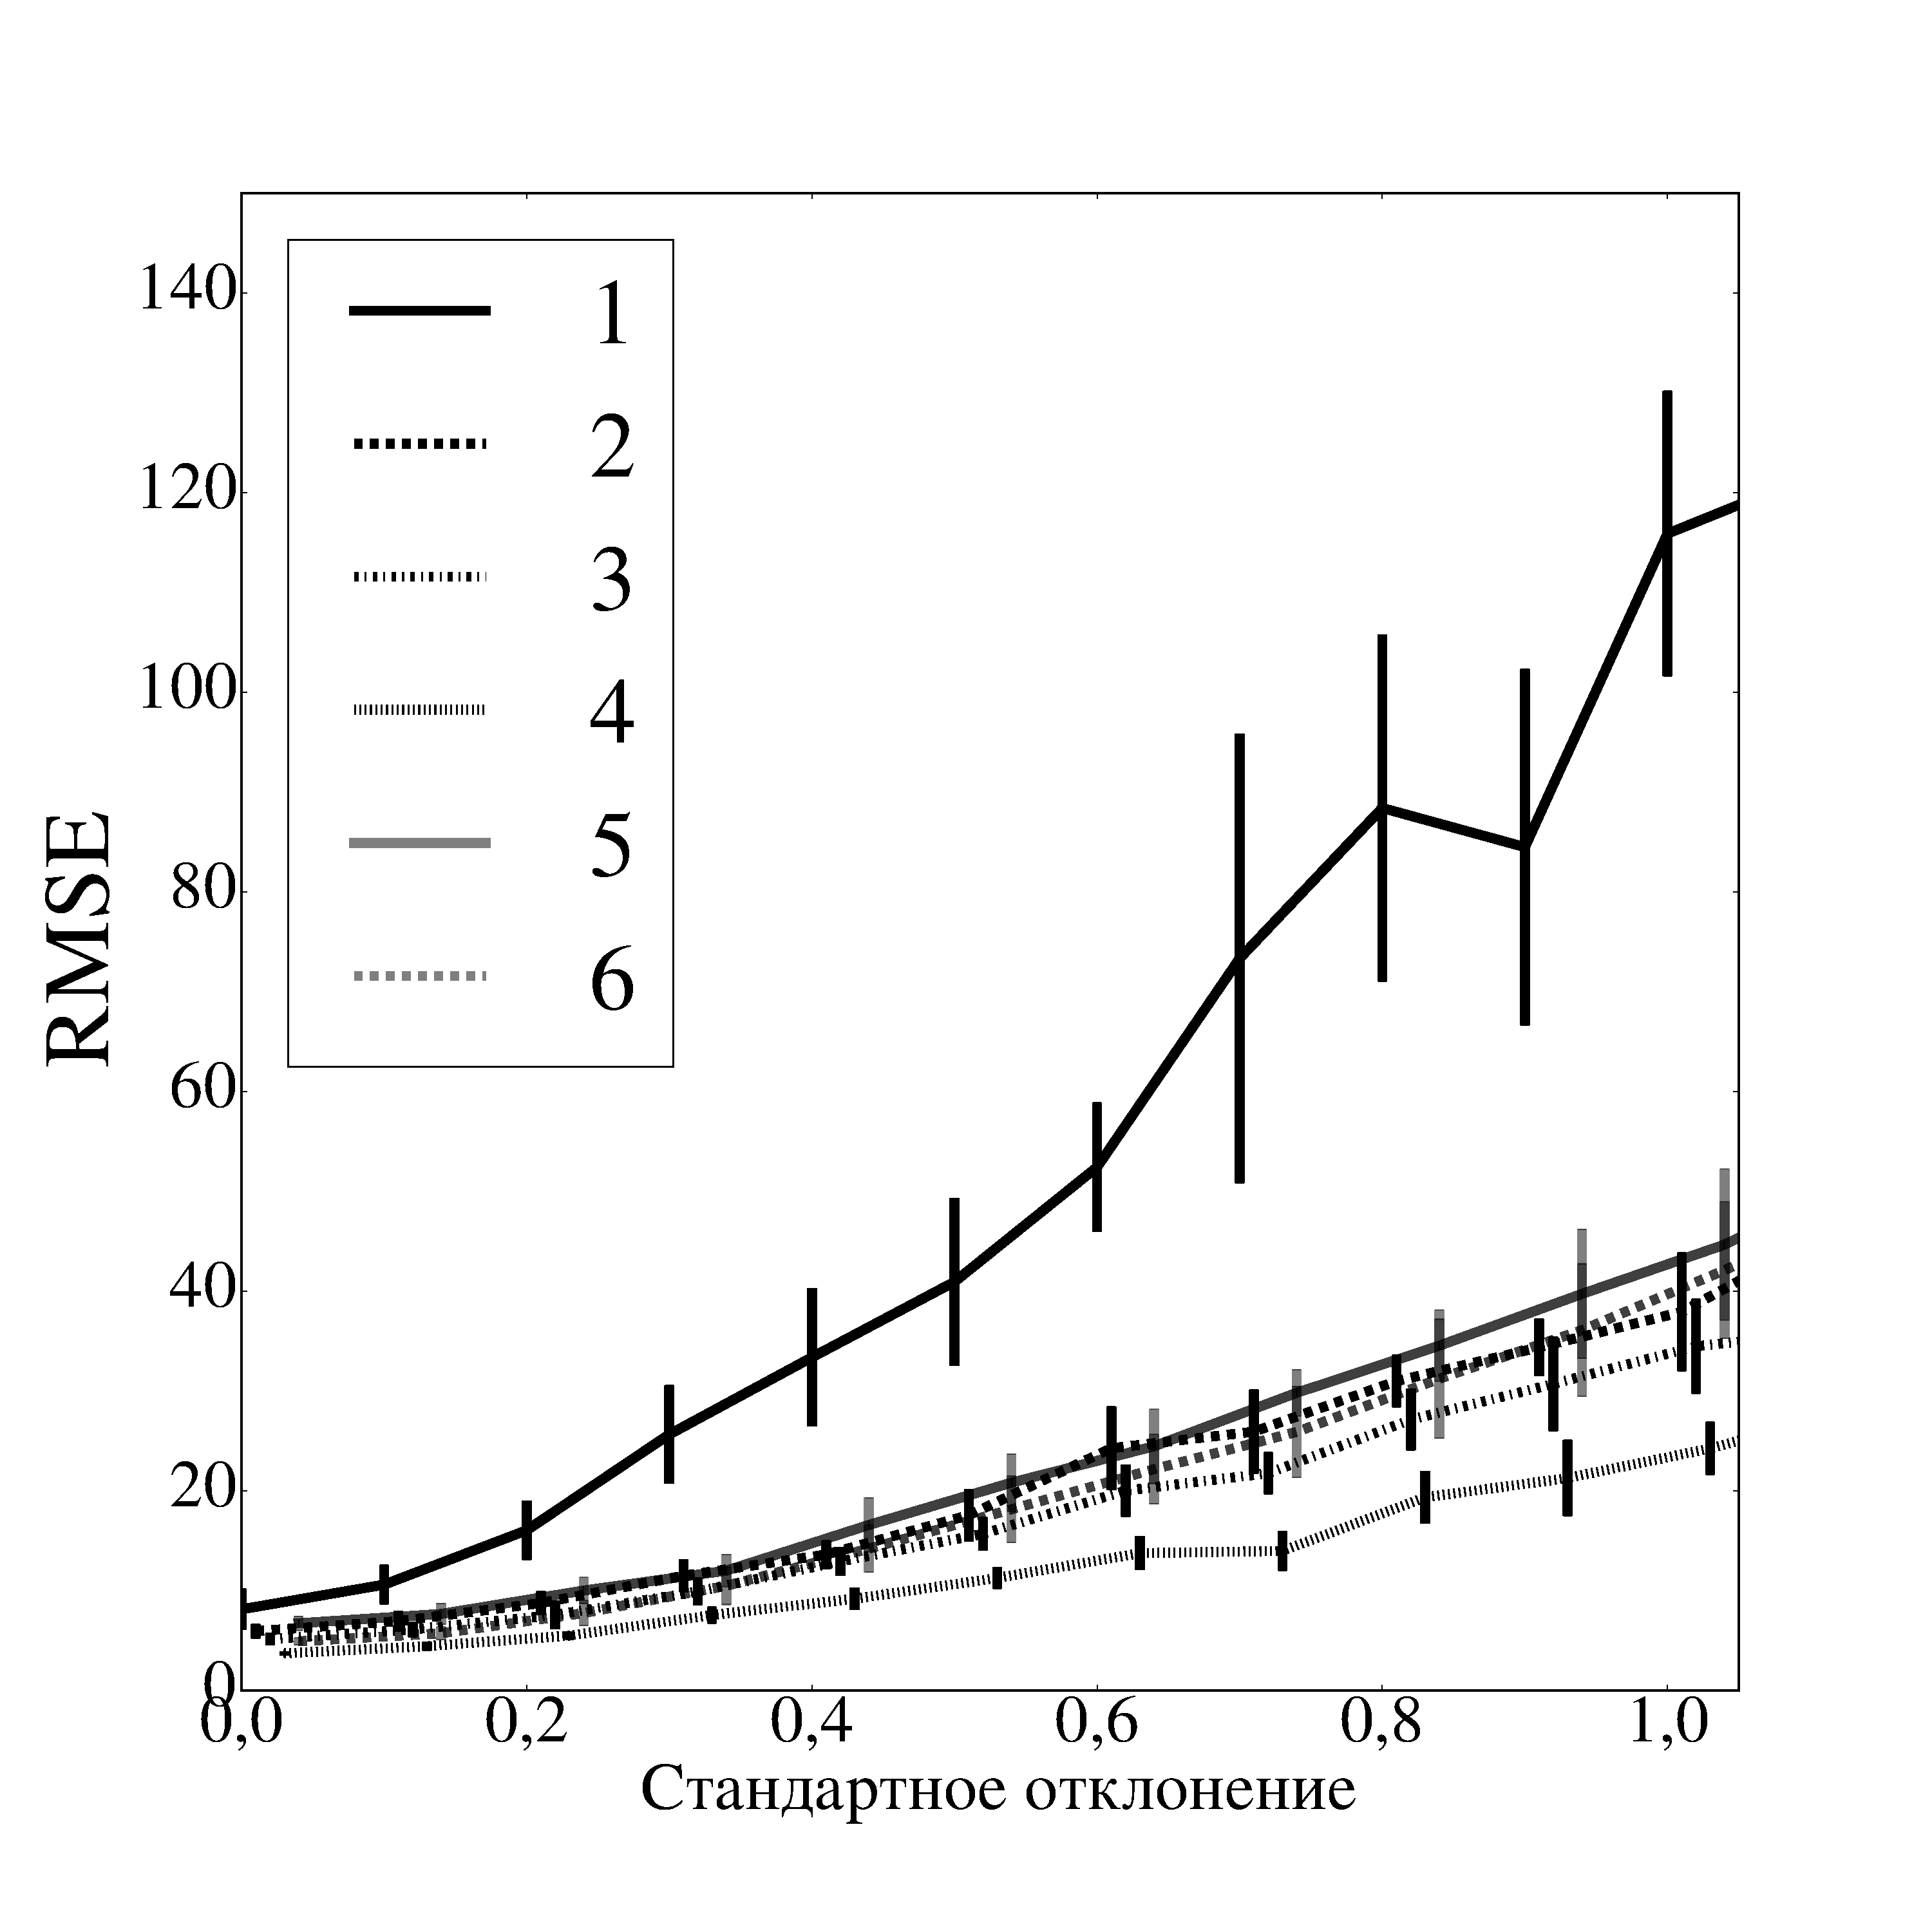
\includegraphics[width=1.0\textwidth]{./plots/var/boston/rmse_data2.pdf}
\endminipage\hfill
\minipage{0.32\textwidth}
\caption*{\textit{б}}
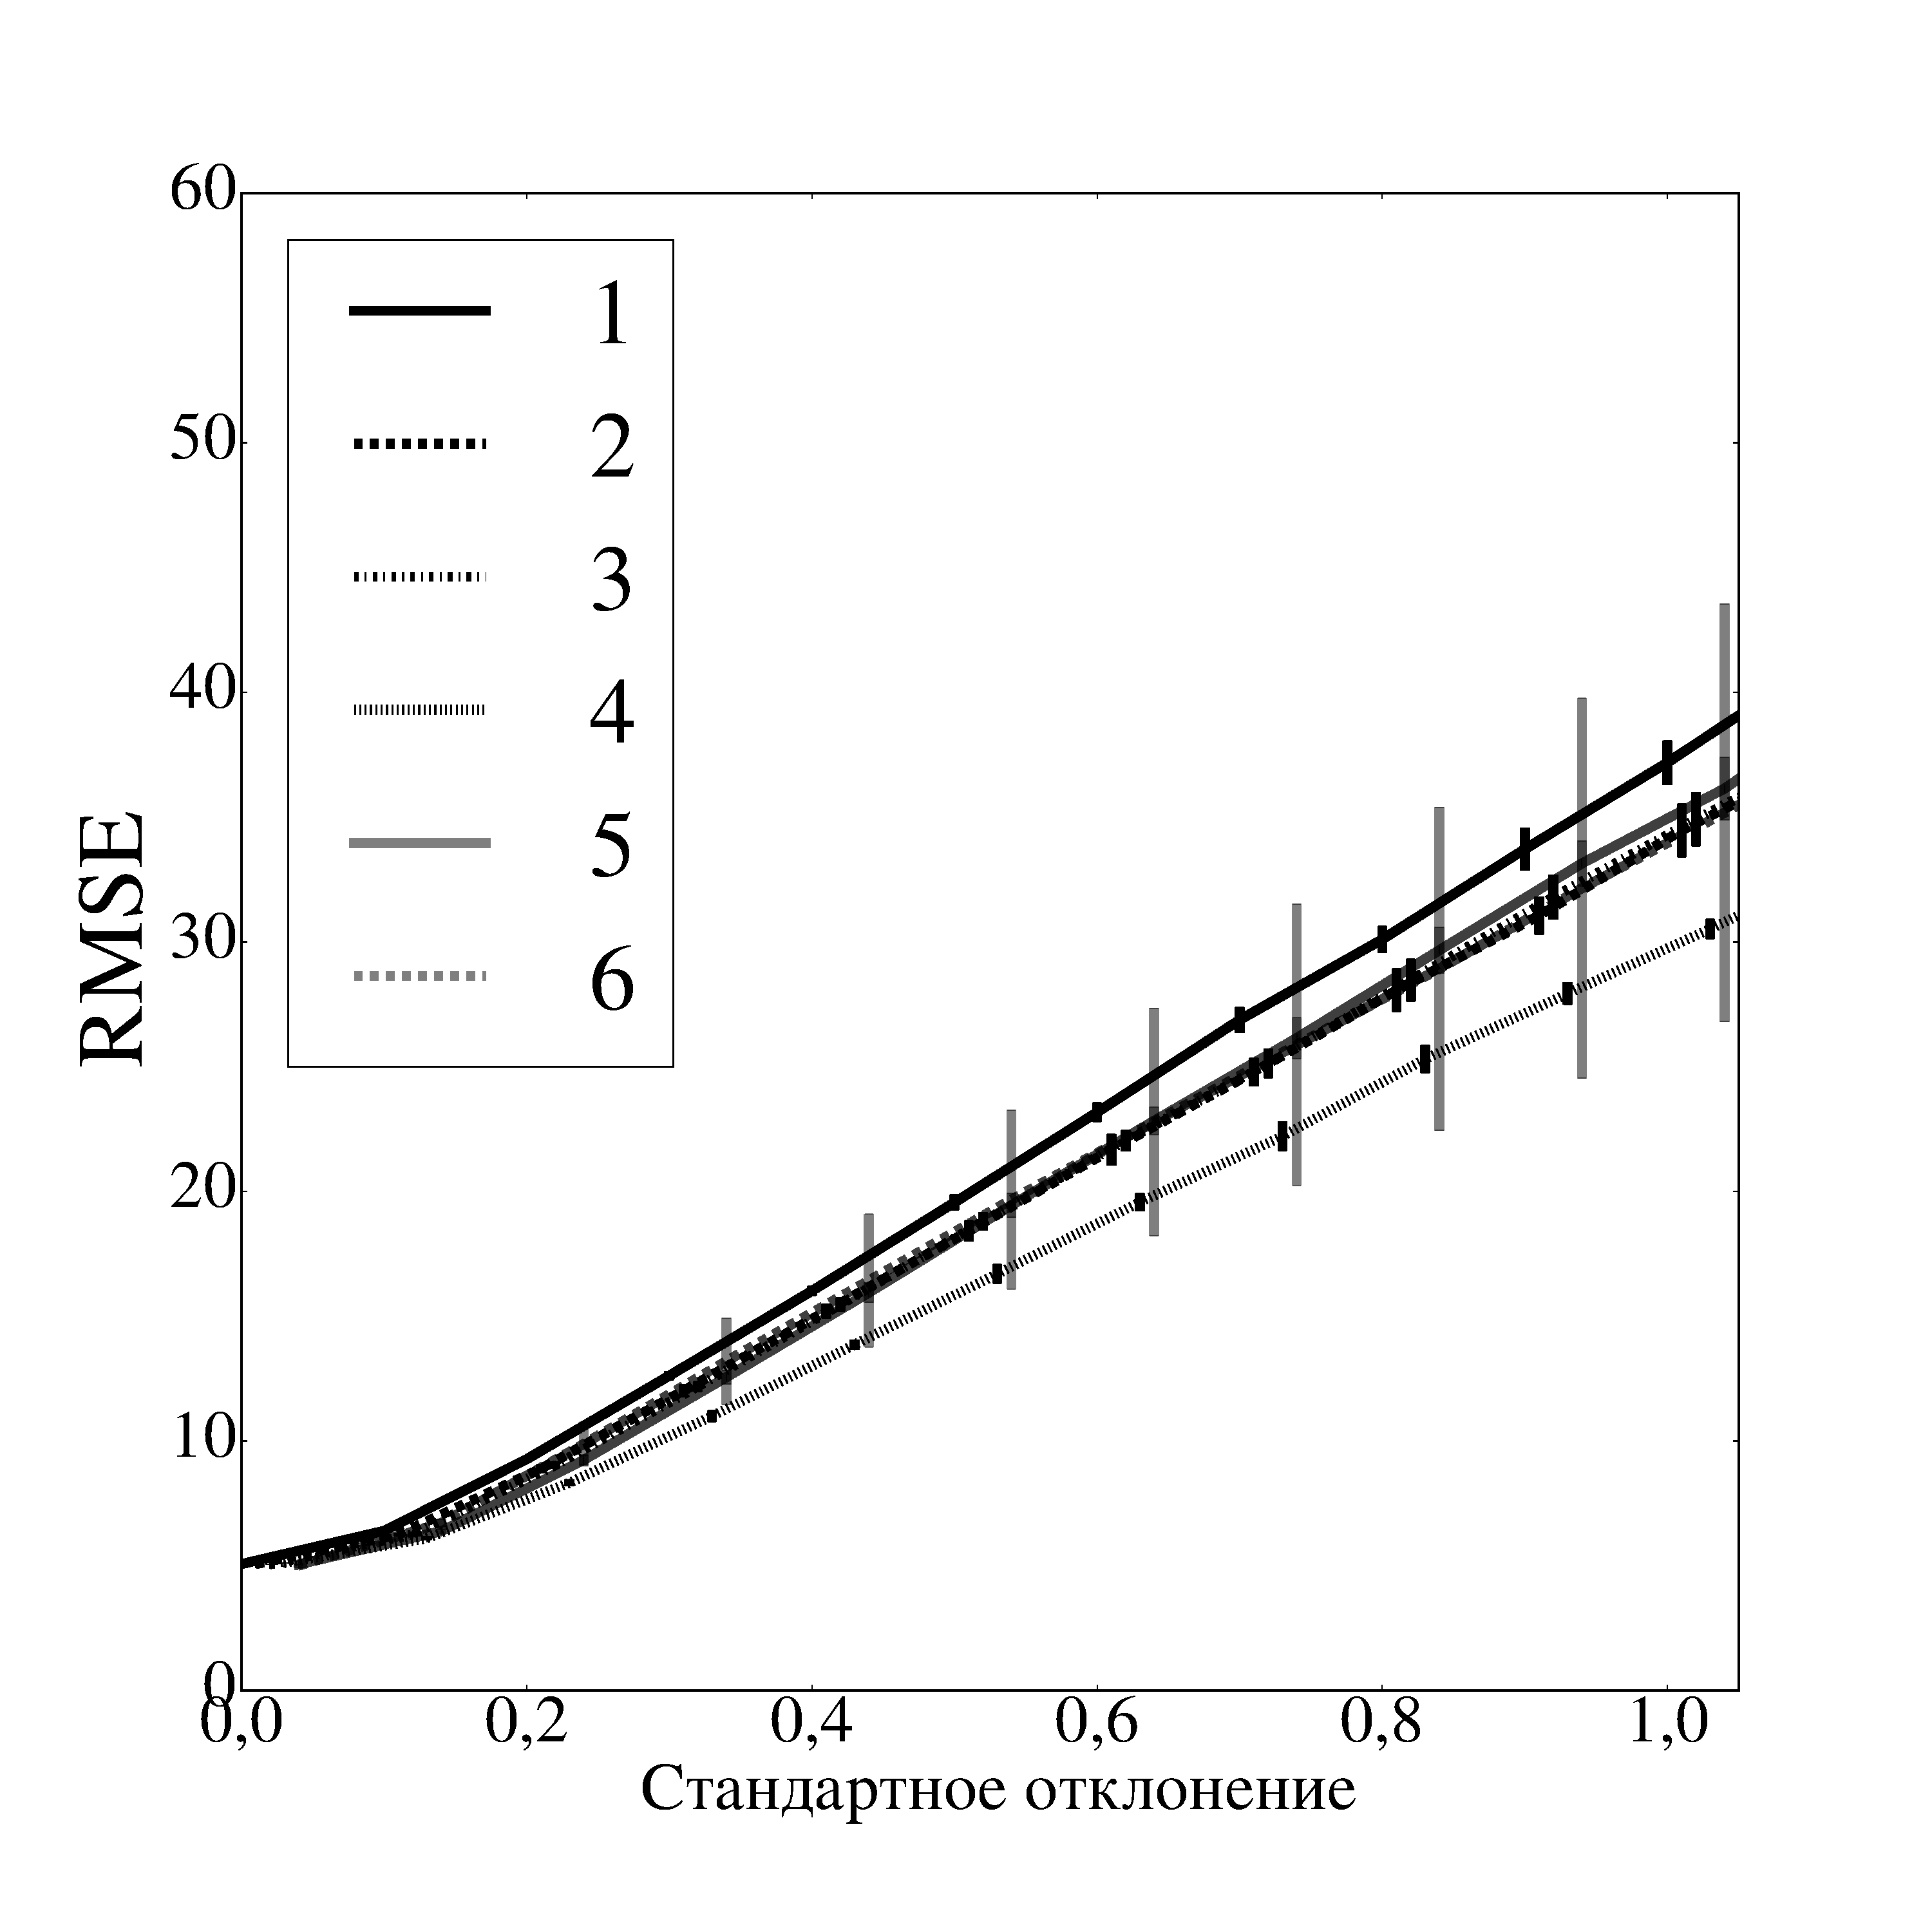
\includegraphics[width=1.0\textwidth]{./plots/var/protein/rmse_data2.pdf}

\endminipage\hfill
\minipage{0.32\textwidth}%
\caption*{\textit{в}}
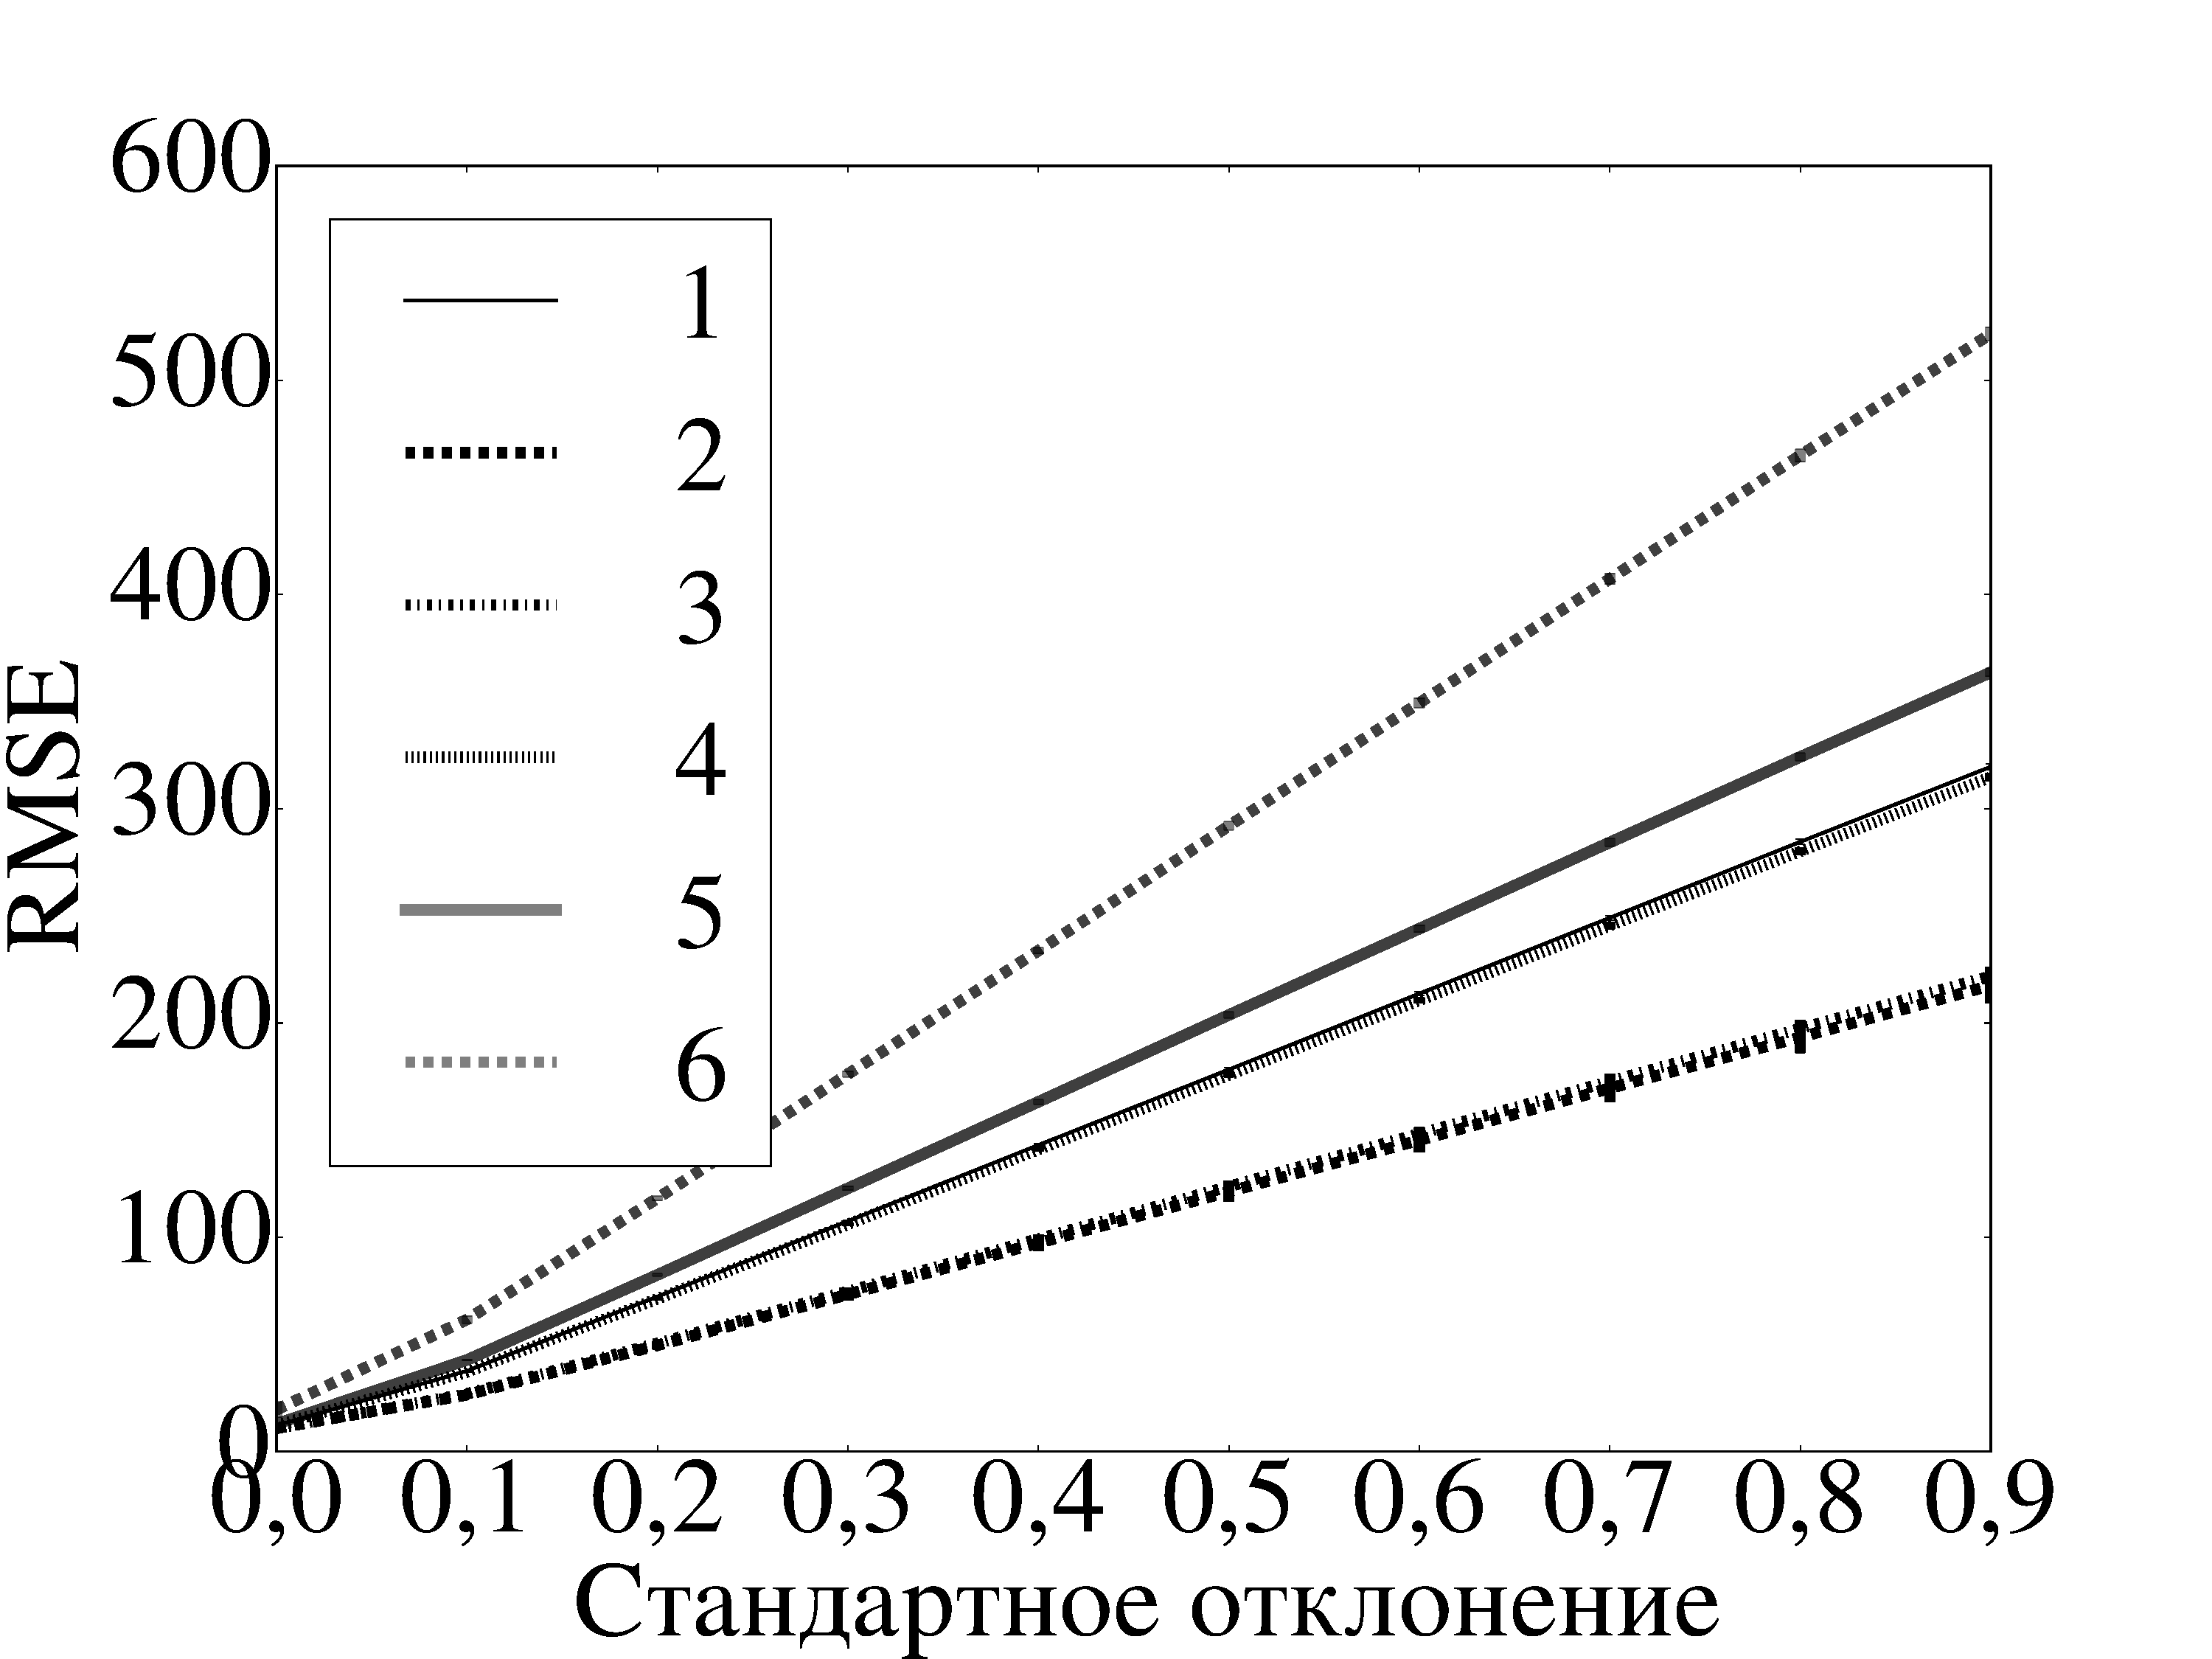
\includegraphics[width=1.0\textwidth]{./plots/var/msd/rmse_data2.pdf}

\endminipage
\caption{ Возмущение выборки для однослойных нейросетей: \textit{а}) Boston Housing, \textit{б}) Protein, \textit{в}) MSD.
}
\label{fig:noise_in_data}
\end{figure}




\begin{table}[!htbp]
\captionsetup{justification=raggedright,singlelinecheck=false}
\label{table1}
\caption{Описание выборок для экспериментов  по выбору моделей}
\footnotesize
\centering

\begin{tabular}{ | p{2cm} |p{2cm} | p{2cm} | p{2cm} | p{2cm} | p{2cm} | }
\hline
Выборка $\mathfrak{D}$ & Интервал валидации, $\tau_\textnormal{val}$ & Количество объектов, $m$ & Количество признаков, $n$ & Размер подвыборки, $\hat{m}$ &  Размер скрытого слоя, $n_1$ \\
\hline
Boston Housing & 100 & 506 & 13 & $\hat{m} = m$ & 50 \\
\hline
Protein & 1000 & 45000 & 9 & $\hat{m} = 200$ & 100 \\
\hline
MSD & 1000& 5000 & 91 & $\hat{m} = 50$ & 100\\
\hline
MNIST & 100  & 500 & 50 & $\hat{m} = 100$ & 50\\ 
\hline
\end{tabular}
\end{table}


\newcommand{\specialcell}[2][c]{%
  \begin{tabular}[#1]{@{}c@{}}#2\end{tabular}}

\begin{table}[htbp!]
\captionsetup{justification=raggedright,singlelinecheck=false}
\centering
\label{table2}
\caption{Результаты эксперимента по выбору моделей}
\footnotesize
\begin{tabular}{ | c | c | c | c | c | c | c |}

\hline
&\multicolumn{6}{|c|}{Алгоритмы}  \\
\hline
Выборка $\mathfrak{D}$ & 1 & 2 & 3 & 4 & 5 & 6 \\
\hline
\multicolumn{7}{|c|}{Результаты, RMSE/Accuracy}  \\

\hline
\specialcell{ Boston,  \\один  слой} & 8,1  $\pm$ 2,0 & 5,9 $\pm$ 0,7 & 5,2 $\pm$ 0,6 & $\mathbf{3,7 \pm 0,2}$ & 6,7 $\pm$ 0,7 & 5,0 $\pm$ 0,4 \\
\hline
Boston, 3 слоя & 7,1 $\pm$ 1,3 & 4,3 $\pm$ 0,1 & 4,4 $\pm$ 0,4 & $\mathbf{3,2 \pm 0,06}$ & 4,6 $\pm$ 0,4 & 6,8 $\pm$ 1,6 \\
\hline
Protein & 5,1 $\pm$ 0,0 & 5,1 $\pm$ 0,0 & 5,1 $\pm$ 0,0 & 5,1 $\pm$ 0,0 & 5,1 $\pm$ 0,0 & $\mathbf{5,0 \pm 0,1}$ \\
\hline
MSD & 12,2 $\pm$ 0,0 & $\mathbf{10,9 \pm 0,1}$ & $\mathbf{10,9 \pm 0,1}$ & 12,2 $\pm$ 0,0 & 12,9 $\pm$ 0,0 & 19,6 $\pm$ 3,6  \\
\hline
MNIST & 0,985 $\pm$ 0,002 & 0,984 $\pm$ 0,002 & $\mathbf{0,986 \pm 0,002}$ & 0,914 $\pm$ 0,005 & 0,979 $\pm$ 0,003 & 0,971 $\pm$ 0,001 \\
\hline

\multicolumn{7}{|c|}{Результаты, $\textnormal{RMSE/Accuracy}_{0,5}$}  \\
\hline
\specialcell{ Boston,  \\один  слой} & 43,9  $\pm$ 9,4 & 18,6 $\pm$ 2,0 &  15,8 $\pm$ 2,3 & $\mathbf{11,9 \pm 1,1}$ & 20,3 $\pm$ 3,1 & 18,2 $\pm$ 3,3 \\
\hline
Boston, 3 слоя & 23,4 $\pm$ 4,9 & 18,7 $\pm$ 2,8 & 18,3 $\pm$ 3,0 & \bf 9,0 $\pm$ 0,7 & 14,5 $\pm$ 2,6 &  15,2 $\pm$ 2,7 \\
\hline
Protein & 19,5 $\pm$ 0,3 & 18,5 $\pm$ 0,5 & 18,6 $\pm$ 0,3 & $\mathbf{16,7 \pm 0,3}$ & 19,3 $\pm$ 0,6 & 19,7 $\pm$ 3,7  \\
\hline
MSD & 178,3 $\pm$ 0,8 & $\mathbf{121,3 \pm 4,5}$ & 123,7 $\pm$ 2,5 & 175,8 $\pm$ 1,0 & 203,8 $\pm$ 1,4 & 292,0 $\pm$ 2,0 \\
\hline
MNIST & 0,931 $\pm$ 0,004 & 0,929 $\pm$ 0,006 & $\mathbf{0,934 \pm 0,007}$ & 0,857 $\pm$ 0,007 & 0,919 $\pm$ 0,008 & 0,916 $\pm$ 0,004 \\
\hline


\multicolumn{7}{|c|}{Результаты, $\textnormal{RMSE/Accuracy}_{1,0}$}  \\
\hline
\specialcell{ Boston,  \\один  слой} & 120,9 $\pm$ 33,4 & 42,5 $\pm$ 6,3 & 32,5 $\pm$ 6,0 & $\mathbf{25,7 \pm 3,2}$ & 42,4 $\pm$ 5,7 & 41,3 $\pm$ 6,3  \\
\hline
Boston, 3 слоя & 46,1 $\pm$ 15,8 & 40,5 $\pm$ 5,3 & 38,6 $\pm$ 8,0 & \bf 16,5 $\pm$ 2,5 & 30,4 $\pm$ 7,9 & 26,2 $\pm$ 6,9 \\
\hline
Protein & 37,0 $\pm$ 0,8 & 34,4 $\pm$ 1,1 & 35,0 $\pm$ 1,0 & $\mathbf{30,6 \pm 0,6}$ & 36,6 $\pm$ 1,1 & 35,0 $\pm$ 8,1 \\
\hline
MSD & 319,6 $\pm$ 1,4 & $\mathbf{217,5 \pm 8,2}$ & 221,9 $\pm$ 4,2 & 314,8 $\pm$ 1,8 & 363,7 $\pm$ 1,9 & 521,6 $\pm$ 3,1  \\
\hline
MNIST & $\mathbf{0,814 \pm 0,010 }$& 0,808 $\pm$ 0,010 &  0,812 $\pm$ 0,008 & 0,772 $\pm$ 0,010 & 0,802 $\pm$ 0,009 & 0,800 $\pm$ 0,009 \\
\hline


\multicolumn{7}{|c|}{Сходимость алгоритмов, тыс. итераций  }  \\
%Выборка $\mathbf{X}$ & Алгоритм 1 & Алгоритм 2 & Алгоритм 3 & Алгоритм 4 & Алгоритм 5 & Алгоритм 6 \\
\hline
\specialcell{ Boston,  \\один  слой} &  25 & 25 & 25 & 14 & 10 & 27 \\
\hline
Boston, 3 слоя &  25 & 4 & 9 & 10 & 1 & 6 \\
\hline
Protein &   60 & 40 & 80 & 40 & 75 & 85 \\
\hline
MSD &  250 & 330 & 335 &  250 & 460 & 120  \\
\hline
MNIST &  1 & 6 & 3 &  13 & 3 & 25  \\
\hline
\end{tabular}
\end{table}





Модели имеют достаточно большое число параметров, поэтому в ходе оптимизации параметров может произойти переобучение. На выборке Boston Housing базовый алгоритм (1) показал наихудший результат в силу переобучения, при этом алгоритм 4 показал лучший результат по сравнению с алгоритмами 2 и 3. 
В данном случае использование вариационной оценки предпочтительнее алгоритмов, основанных на кросс-валидации. На выборке Protein все алгоритмы показали схожие результаты. На выборке MSD алгоритмы 4,5,6 показали худший результат в сравнении с алгоритмами, использующими валидационную подвыборку. Наихудший результат показал алгоритм 6, что говорит о значительном отличии апостериорного распределения параметров~\eqref{eq:posterior} от нормального.  

Алгоритм 6 показал низкое качество~\eqref{eq:rmse} при возмущении объектов выборки {в большинстве экспериментов}. В {трех} экспериментах наилучшие показатели по данному критерию показал алгоритм 4. Заметим, что алгоритм 5, являющийся модификацией алгоритма 4, показал худшие результаты как по RMSE, так и по RMSE при возмущении объектов выборки. 
{На выборке MNIST алгоритм 4 показал результаты значительно хуже остальных алгоритмов. В целом результаты по данному алгоритму схожи с результатами, описанными в~\cite{early}: в отличие от алгоритма 5 алгоритм 4, основанный на стохастическом градиентном спуске, дает заниженную оценку правдоподобия при приближении параметров к точке экстремума. } Алгоритм 5, основанный на динамике Ланжевена, также показал худшее время сходимости~{на выборках MSD и Protein}. Возможным дальнейшим улучшением качества этого алгоритма является введение дополнительной корректирующей матрицы, обеспечивающей лучшее время сходимости параметров к апостериорному распределению параметров~\cite{langevin}.

Программное обеспечение для проведения экспериментов и проверки результатов  находится в~\cite{my_src}. 













\clearpage


\chapter{Оптимизация гиперпараметров в задаче выбора модели}

Задача оптимизации гиперпараметров зависит как от критерия выбора модели, так и от метода оптимизации параметров модели.
Проиллюстрируем задачу оптимизации гиперпараметров \textit{двусвзяным байесовским выводом}. Для дальнейшей формализации задачи положим:
\begin{equation}
\label{eq:bayes0}
	\boldsymbol{\theta} = \mathbf{W}, \quad \mathbf{h} = \text{diag}(\mathbf{A}) = [\alpha_1, \dots, \alpha_u].
\end{equation}

На \textit{первом уровне} байесовского вывода производится оптимизация параметров модели $\mathbf{f}$ по заданной выборке $\mathfrak{D}$:
\begin{equation}
\label{eq:bayes1}
\hat{\boldsymbol{\theta}} = \argmax \bigl(-L(\boldsymbol{\theta}, \mathbf{h})\bigr) = p(\mathbf{W}|\mathbf{X}, \mathbf{y}, \mathbf{A}) = \frac{p(\mathbf{y}|\mathbf{X},\mathbf{W})p(\mathbf{W}|\mathbf{A})}{p(\mathbf{y}|\mathbf{X},\mathbf{A})}.
\end{equation}

На \textit{втором уровне} производится оптимизация апостериорного распределения гиперпараметров $\mathbf{h}$:
\[
p(\mathbf{A}|\mathbf{X}, \mathbf{y}) \propto p(\mathbf{y}|\mathbf{X},\mathbf{A})p(\mathbf{A}),
\]
где знак <<$\propto$>> означает равенство с точностью до нормирующего множителя.

Полагая распределение параметров $p(\mathbf{A})$ равномерным на некоторой большой окрестности, получим задачу оптимизации гиперпараметров:
\begin{equation}
\label{eq:bayes2}
	Q(\boldsymbol{\theta}, \mathbf{h}) = p(\mathbf{y}|\mathbf{X},\mathbf{A}) = \int_{\mathbf{W} \in \mathbb{R}^u} p(\mathbf{y}|\mathbf{X}, \mathbf{W}) p(\mathbf{W}|\mathbf{A}) \to \max_{[\alpha_1, \dots, \alpha_u] \in \mathbb{R}^{n}}.
\end{equation}


В общем виде задача оптимизации гиперпараметров сводится к двухуровневой задаче оптимизации~\eqref{eq:optim}.
Рассмотрим вид переменной $\boldsymbol{\theta}$ и функций $L, Q$ для различных методов выбора модели и оптимизации ее параметров.

\textbf{Базовый метод}
Пусть оптимизация параметров и гиперпараметров производится по всей выборке $\mathfrak{D}$ по одной и той же функции:
$$L(\boldsymbol{\theta}, \mathbf{h}) = Q(\boldsymbol{\theta}) = \text{log}p(\mathbf{y}, \mathbf{W} | \mathbf{X}, \mathbf{A}) = \text{log} p(\mathbf{y}|\mathbf{X}, \mathbf{W})+\text{log}p(\mathbf{W}|\mathbf{A})$$.

Вспомогательная переменная $\boldsymbol{\theta}$, по которой производится оптимизация модели $f$,  соответствует параметрам модели: 
\[
\boldsymbol{\theta} = \mathbf{W}.
\]

\textbf{Кросс-валидация}
Разобьем выборку $\mathfrak{D}$ на $k$ равных частей:
\[
\mathfrak{D} = \mathfrak{D}_1 \sqcup \dots \sqcup \mathfrak{D}_k.
\]


Запустим $k$ оптимизаций модели, каждую на своей части выборки. Положим $\boldsymbol{\theta} = [\mathbf{W}_1, \dots, \mathbf{W}_k]$, где $\mathbf{W}_1, \dots, \mathbf{W}_k$ --- параметры модели при оптимизации $k$.
 
Положим функцию $L$ равной  среднему значению минус логарифма апостериорной вероятности по всем $k-1$ разбиениям $\mathfrak{D}$:
\begin{equation}
\label{eq:cv}
L(\boldsymbol{\theta}, \mathbf{h}) = -\frac{1}{k}\sum_{q=1}^k \bigl(\frac{k}{k-1}\text{log}p(\mathbf{y} \setminus \mathbf{y}_q|\mathbf{X}\setminus \mathbf{X}_q, \mathbf{W}_q) + \text{log}p(\mathbf{W}_q|\mathbf{A})\bigr).
\end{equation}

Положим функцию $Q$ равной среднему значению правдоподобия выборки по частям выборки $\mathfrak{D}_q$, на которых не проходила оптимизация параметров:
\[
Q(\boldsymbol{\theta}, \mathbf{h}) = \frac{1}{k}\sum_{q=1}^k k\text{log}p(\mathbf{y}_q|\mathbf{X}_q, \mathbf{W}_q).
\]

\textbf{Вариационная оценка правдоподобия}
Положим $L=-Q$, равной вариационной оценке правдоподобия модели:
\begin{equation} 
\label{eq:elbo}
\text{log}~p(\mathbf{y}|\mathbf{X},\mathbf{A})  
\geq 
-\text{D}_\text{KL} \bigl(q(\mathbf{W})||p(\mathbf{W}|\mathbf{A})\bigr) + \int_{\mathbf{W}} q(\mathbf{W})\text{log}~{p(\mathbf{y}|\mathbf{X},\mathbf{W},\mathbf{A})} d \mathbf{W}  \approx
\end{equation}
\[
\approx \sum_{i=1}^m \text{log}~p({y}_i|\mathbf{x}_i, \mathbf{W}_i) - D_\text{KL}\bigl(q (\mathbf{W}) || p (\mathbf{W}|\mathbf{A})\bigr) = -L(\boldsymbol{\theta}, \mathbf{h}) = Q(\boldsymbol{\theta}),
\]

где $q$ --- нормальное распределение с диагональной матрицей ковариаций:
\begin{equation}
\label{eq:diag}
	q \sim \mathcal{N}(\boldsymbol{\mu}_q, \mathbf{A}^{-1}_q),
\end{equation}
где $\mathbf{A}_q = \text{diag}[\alpha^q_1, \dots, \alpha^q_u]^{-1}$ --- диагональная матрица ковариаций, $\boldsymbol{\mu}_q$ --- вектор средних компонент.
Расстояние $D_\text{KL}$ между двумя гауссовыми величинами задается как 
\[
	D_\text{KL}\bigl(q (\mathbf{W}) || p (\mathbf{W}|\mathbf{f})\bigr) = \frac{1}{2} \bigl( \text{Tr} [\mathbf{A}\mathbf{A}^{-1}_q] + (\boldsymbol{\mu} - \boldsymbol{\mu}_q)^\mathsf{T}\mathbf{A}(\boldsymbol{\mu} - \boldsymbol{\mu}_q) - u +\text{ln}~|\mathbf{A}^{-1}| - \text{ln}~|\mathbf{A}_q^{-1}| \bigr).
\]

В качестве оптимизируемых параметров $\boldsymbol{\theta}$ выступают параметры распределения $q$:
\[
\boldsymbol{\theta} = [\alpha_1, \dots, \alpha_u, {\mu}_1,\dots,{\mu}_u].
\]




\section{Градиентные методы оптимизации гиперпараметров}
Рассмотрим случай, когда оптимизация~\eqref{eq:main2} параметров $\boldsymbol{\theta}$ производится с использованием градиентных методов. 

Рассмотрим оператор градиентного спуска, производящий $\eta$ шагов оптимизации:
\begin{equation}
\label{eq:gd}
	 \hat{\boldsymbol{\theta}} = T \circ T \circ \dots \circ T(\boldsymbol{\theta}_0, \mathbf{h}) = T^\eta(\boldsymbol{\theta}_0, \mathbf{h}),
\end{equation}
где 
$$
	T(\boldsymbol{\theta}, \mathbf{h}) =\boldsymbol{\theta} - \gamma \nabla L(\boldsymbol{\theta}, \mathbf{h}), 
$$
$\gamma$ --- длина шага градиентного спуска, $\boldsymbol{\theta}_0$ --- начальное значение параметров $\boldsymbol{\theta}$. В данной работе в качестве опреатора оптимизации параметров модели выступает стохастический градиентный спуск:
\[
T(\boldsymbol{\theta}, \mathbf{h})_\text{SGD} =\boldsymbol{\theta} - \gamma \nabla L(\boldsymbol{\theta}, \mathbf{h})|_{\mathfrak{D} = \hat{\mathfrak{D}}},
\]
где $\hat{\mathfrak{D}}$ --- случайная подвыборка исходной выборки $\mathfrak{D}$.

Перепишем задачу оптимизации~\eqref{eq:main}, ~\eqref{eq:main2} в следующем виде
\begin{equation}
\label{eq:optim}
	\hat{\mathbf{h}} = \argmax_{\mathbf{h} \in \mathbb{R}^h} Q( T^\eta(\boldsymbol{\theta}_0, \mathbf{h})),
\end{equation}
где $\boldsymbol{\theta}_0$ --- начальное значение параметров $\boldsymbol{\theta}$.

Оптимизационную задачу~\eqref{eq:optim} предлагается решать с использованием градиентного спуска. Вычисление градиента от функции $Q( T^\eta(\boldsymbol{\theta}_0, \mathbf{h}))$ по гиперпараметрам $\mathbf{h}$ является вычислительно сложным в силу внутренней процедуры оптимизации $T(\boldsymbol{\theta}_0, \mathbf{h})$. 
Общая схема  оптимизации гиперпараметров представлена следующим образом:
\begin{enumerate}
\item От 1 до  $l$:
\item Инициализировать парметры $\boldsymbol{\theta}$ при условии гиперпараметров $\mathbf{h}$.
\item Приближенно решить задачу оптимизации~\eqref{eq:optim} и получить новый вектор параметров $\mathbf{h}'$
\item $\mathbf{h} = \mathbf{h}'$.
\end{enumerate}
где $l$ --- количество итераций оптимизации гиперпараметров. Рассмотрим методы приближенного решения данной задачи оптимизации.



\textbf{Жадный алгоритм}
В качестве  правила обновления вектора гиперпараметров $\mathbf{h}$ на каждом шаге оптимизации~\eqref{eq:gd} выступает градиентный спуск с учетом обновления параметров $\boldsymbol{\theta}$ на данном шаге:
\[
	\mathbf{h}' = \mathbf{h} - \gamma_{\mathbf{h}} \nabla_{\mathbf{h}}  Q \bigl(T(\boldsymbol{\theta}, \mathbf{h}) , \mathbf{h}\bigr) = \mathbf{h} - \gamma_{\mathbf{h}} \nabla_{\mathbf{h}}  Q\bigl(\boldsymbol{\theta} - \gamma \nabla L(\boldsymbol{\theta}, \mathbf{h}), \mathbf{h})\bigr),
\]
где $\gamma_{\mathbf{h}}$ --- длина шага оптимизации гиперпараметров.

\textbf{Алгоритм HOAG}
Предлагается получить приближенное значения градиента гиперпараметров $\nabla_{\mathbf{h}} Q \bigl(T^\eta(\boldsymbol{\theta}_0, \mathbf{h})\bigr)$ на основе следующей формулы:
\[
\nabla_{\mathbf{h}} Q \bigl(T^\eta(\boldsymbol{\theta}_0, \mathbf{h})\bigr) = \nabla_{\mathbf{h}} Q(\boldsymbol{\theta}, \mathbf{h}) - (\nabla^2_{\boldsymbol{\theta}, \mathbf{h}} L(\boldsymbol{\theta}, \mathbf{h}))^\text{T}\mathbf{H}(\boldsymbol{\theta})^{-1}\nabla_{\boldsymbol{\theta}} Q(\boldsymbol{\theta}, \mathbf{h}),
\]
где $\mathbf{H}$ --- гессиан функции $L$ по параметрам $\boldsymbol{\theta}$.

Процедура получения приближенного значения градиента гиперпараметров $\nabla_{\mathbf{h}} Q$  производится итеративно:
\begin{enumerate}
\item Провести $\eta$ шагов оптимизации: $\boldsymbol{\theta} = T(\boldsymbol{\theta}_0, \mathbf{h})$.
\item Решить линейную систему для вектора $\boldsymbol{\lambda}$: $\mathbf{H}(\boldsymbol{\theta})\boldsymbol{\lambda} =  \nabla_{\boldsymbol{\theta}} Q(\boldsymbol{\theta}, \mathbf{h})$.
\item Приближенное значение градиентов гиперпараметра вычисляется как: $\hat{\nabla}_{\mathbf{h}}Q = \nabla_{\mathbf{h}}Q(\boldsymbol{\theta}, \mathbf{h}) -\nabla_{\boldsymbol{\theta}, \mathbf{h}} L(\boldsymbol{\theta}, \mathbf{h})^T\boldsymbol{\lambda}$.
\end{enumerate}

Итоговое правило обновления:
\begin{equation}
\label{eq:update_hyper}
\mathbf{h}' = \mathbf{h} - \gamma_{\mathbf{h}} \hat{\nabla}_{\mathbf{h}}Q.
\end{equation}

В данной работе для приближенного решения  шага 2 алгоритма HOAG используется стохастический градиентный спуск в силу сложности вычисления гессиана $\mathbf{H}(\boldsymbol{\theta})$.


\textbf{Алгоритм DrMad}

Для получения градиента от оптимизируемой функции $Q$ как от функции от начальных параметров $\boldsymbol{\theta}_0$ предлагаетя пошагово восстановить $\eta$ шагов оптимизации $T(\boldsymbol{\theta}_0)$ в обратном порядке аналогично методу обратного распространения ошибок. Для упрощения данной процедуры вводится предположение,что траектория изменения параметров $\boldsymbol{\theta}$ линейна:
\begin{equation}
\label{eq:mad_lin}
\boldsymbol{\theta}^\tau = \boldsymbol{\theta}_0 + \frac{\tau}{\eta} T(\boldsymbol{\theta}).
\end{equation}

Алгоритм вычисления приближенного значения градиента $\nabla \mathbf{h}$ является частным случаем алгоритма обратного распространения ошибки и представим в следующем виде:
\begin{enumerate}
\item Провести $\eta$ шагов оптимизации: $\boldsymbol{\theta} = T(\boldsymbol{\theta}_0, \mathbf{h})$.
\item Положим $\hat{\nabla} \mathbf{h} = \nabla_\mathbf{h} Q(\boldsymbol{\theta}, \mathbf{h}).$ 
\item Положим $d\mathbf{v} = \mathbf{0}.$
\item Для $\tau = \eta \dots 1 $ повторить:
\item Вычислить значения параметров $\boldsymbol{\theta}^\tau$\eqref{eq:mad_lin}.
\item $d\mathbf{v} =  \gamma \hat{\nabla}_{\boldsymbol{\theta}}$.
\item $\hat{\nabla} \mathbf{h} =  \hat{\nabla} \mathbf{h} - d\mathbf{v}\nabla_{\mathbf{h}} \nabla_{\boldsymbol{\theta}} Q$.
\item $\hat{\nabla} \boldsymbol{\theta}  = \hat{\nabla} \boldsymbol{\theta}  - d\mathbf{v}\nabla_{\boldsymbol{\theta}} \nabla_{\boldsymbol{\theta}} Q$.
\end{enumerate}

Итоговое правило обновления гиперпараметров аналогично~\eqref{eq:update_hyper}.
В работе~\cite{hyper_mad} отмечается неустойчивость алгоритма при высоких значениях длины шага градиентного спуска $\gamma$. Поэтому вместо исходного правила~\eqref{eq:mad_lin} в данной работе первые 5\% значений параметров не рассматриваются, а также учитывается только каждый $\tau_k$ шаг оптимизации:
\begin{equation}
\label{eq:mad_lin2}
\boldsymbol{\theta}^\tau = \boldsymbol{\theta}_{\tau_0} + \frac{\tau}{\eta} T(\boldsymbol{\theta}), \quad \tau \in \{\tau_0,\dots,\eta\}, \tau \text{ mod } \tau_k = 0,
\end{equation}
где $\tau_0 = [0.05 \cdot \eta]$.


\begin{table}
\small
% Алгоритм & Тип алгоритм & Время & Плюсы & Минусы 

\begin{tabularx}{\textwidth}{|X|X|X|X|}
\hline
\bf Алгоритм & \bf Тип алгоритма & \bf Сложность работы одной итерации & \bf Предположения для корректности  \\ 
Случайный поиск & стохастический & $O(\eta s |\hat{\mathfrak{D}}|)$& -  \\ \hline
Жадный алгоритм~\cite{hyper_greed} & градиентный & $O(\eta (s+h) |\hat{\mathfrak{D}}|)$ & $\mathbf{H}(\boldsymbol{\theta}) = \mathbf{I}$  \\ \hline
HOAG~\cite{hyper_hoag} & градиентный & $O(\eta s |\hat{\mathfrak{D}}| + h^2 |\hat{\mathfrak{D}}| + \text{o}),$ где $o$ --- время решения уравнения пункте 3&  первые производные $Q$ и вторые производные $L$ --- липшецевы;  $\text{det}\mathbf{H} \neq \mathbf{0}$;  \\ \hline
DrMAD~\cite{hyper_mad} & градиентный &$O(\eta s |\hat{\mathfrak{D}}|)$ & Траектория оптимизации параметров $\boldsymbol{\theta}$ = $\boldsymbol{\theta}_0, \dots \boldsymbol{\theta}_\eta$ --- линейная \\ \hline
\end{tabularx}

\caption{Основные свойства рассматриваемых алгоритмов}
\label{table:algo_descr}

\end{table}


\clearpage
\chapter{Выбор субоптимальной структуры модели}
В данной главе рассматривается задача выбора структуры модели глубокого обучения. Предлагается ввести вероятностные предположения о распределениях параметров и структуры модели. 
Проводится градиентная оптимизация параметров и гиперпараметров модели на основе байесовского вариационного вывода.  В качестве оптимизируемой функции для гиперпараметров модели предлагается обобщенная функция обоснованности. Показано, что данная функция позволяет проводить оптимизацию, соответствующую нескольким критериям выбора структуры модели: методу максимального правдоподобия, последовательному увеличению и снижению сложности модели, полному перебору структуры модели, а также получению максимума вариационной оценки обоснованности модели. Решается двухуровневая задача оптимизации: на первом уровне проводится оптимизация нижней оценки обоснованности модели по вариационным параметрам модели. На втором уровне проводится оптимизация гиперпараметров модели.

\section{Вероятностная модель}
Определим априорные распределения параметров и структуры модели следующим образом.
Пусть параметры модели распределены нормально с нулевым средним:
\[
    \mathbf{w}^{i,j}_k \sim \mathcal{N}\bigl(\mathbf{0}, \gamma^{i,j}_k(\mathbf{A}^{i,j}_k)^{-1}\bigr),
\]
где $ (\mathbf{A}^{i,j}_k)^{-1}$ --- диагональная матрица. Апирорное распределение $p(\mathbf{w}|\boldsymbol{\Gamma}, \mathbf{h})$ параметров $\mathbf{w}^{i,j}_k$ зависит не только от гиперпараметров $\mathbf{A}_k^{i,j}$, но и от структурного параметра $\gamma^{i,j}_k$.


В качестве априорного распределения для структуры $\boldsymbol{\Gamma}$ предлагается использовать произведение распределений Gumbel-Softmax~\cite{gs}:
\[
    p(\boldsymbol{\Gamma}|\mathbf{h},\boldsymbol{\lambda}) = \prod_{(j,k) \in E} p(\boldsymbol{\gamma}^{j,k}|\mathbf{s}, \lambda_\text{temp}),
\]
где для каждого структурного параметра $\boldsymbol{\gamma}$ с количеством базовых функций $K$ вероятность $p(\boldsymbol{\gamma}|\mathbf{s}, \lambda_\text{temp})$ определна следующим образом:
\[
    p(\boldsymbol{\gamma}|\mathbf{s}, \lambda_\text{temp}) = (K-1)!\lambda_{\text{temp}}^{K-1}\prod_{l=1}^K s_l\gamma_l^{-\lambda_\text{temp} -1} \left(\sum_{l=1}^K s_l\gamma_l^{-\lambda_\text{temp}}\right)^{-K},
\]
где $\mathbf{s} \in (0,\infty)^K$ --- гиперпараметр, отвечающий за смещенность плотности распределения относительно точек симплекса на $K$ вершинах, $\lambda_{\text{temp}}$ --- метапараметр температуры, отвечающий за концентрацию плотности вблизи вершин симплекса или в центре симплекса.

Перечислим свойства, которыми обладает распределение Gumbel-Softmax:
\begin{enumerate}
\item Реализацию $\hat{\gamma}_l,$ т.е. $l$-й компоненты случайной величины $\boldsymbol{\gamma}$  можно породить следующим образом:
\[
    \hat{\gamma}_l = \frac{\text{exp}(\text{log}s_l+\hat{g}_l)/\lambda_{\text{temp}}}{\sum_{l'=1}^{K}\text{exp}(\text{log}s_{l'}+\hat{g}_{l'})/\lambda_{\text{temp}}},
\]
где $\hat{\mathbf{g}} \sim -\text{log}\bigl(-\text{log}~\mathcal{U}(0,1)^K\bigr).$ 

\item Свойство округления: $p(\gamma_{l_1} > \gamma_{l_2}, l_1\neq l_2|\mathbf{s}, {\lambda}_\text{temp}) = \frac{s_l}{\sum_{l'}s_{l'}}.$

\item При устремлении температуры к нулю реализация случайной величины концентрируется на вершинах симплекса:
\[
    p(\lim_{\lambda_{\text{temp}} \to 0}  \gamma_{l} = 1|\mathbf{s}, {\lambda}_\text{temp})  = \frac{s_l}{\sum_{l'}s_{l'}}.
\]


\item При устремлении температуры к бесконечности плотность распределения концентрируется в центре симплекса:
\begin{equation}
\label{eq:theorem_gs}
    \lim_{\lambda_{\text{temp}} \to \infty}  p(\boldsymbol{\gamma}|\mathbf{s}, {\lambda}_\text{temp}) = 
    \begin{cases}
    \infty, \boldsymbol{\gamma}_l = \frac{1}{K}, l \in \{1,\dots,K\},\\
    0, \text{ иначе.}
    \end{cases}
\end{equation}
\end{enumerate}

Доказательства первых трех утверждений приведены в~\cite{gumbel}. Докажем утверждение 4.

\begin{proof} 
Формула плотности записывается следующим образом с точностью до множителя:
\[
       \frac{\lambda_{\text{temp}}^{K-1}}{\left(\sum_{l=1}^K s_l\gamma_l^{-\frac{-K-1}{K}\lambda_\text{temp}}\sum_{l'=1}^K [l \neq l']s_l\gamma_l^{-\frac{1}{K}\lambda_\text{temp}}\right)^{K}}
\]


Заметим, что числитель $\lambda_{\text{temp}}^{K-1}$ имеет меньшую скорость сходимости, чем знаменатель. 
Знаменатель является суммой слагаемых вида:
\begin{equation}
\label{eq:gs}
    \left(\frac{\prod_{l' \neq l} \gamma_{l'}^{\frac{1}{K}}}{\gamma_l^{\frac{K-1}{K}}}\right)^{\lambda_{\text{temp}}}.
\end{equation}
Пусть хотя бы для одного $l$: $\gamma_l \neq \frac{1}{K}$. Пусть $l'$ соответствует индексу максимальной компоненты вектора $\boldsymbol{\gamma}$.
Для $l=l'$ предел выражения~\eqref{eq:gs} при $\lambda_{\text{temp}}$ стремится к бесконечности. Для $l\neq l'$ предел выражения~\eqref{eq:gs} при $\lambda_{\text{temp}}$ стремится к нулю. Возводя сумму пределов в степень $-K$ получаем предел плотности, равный нулю.

Пусть $\boldsymbol{\gamma} = \frac{1}{K}$.
Тогда выражение с точностью до множителя упрощается до $\lambda^{K-1}$. Предел данного выражения стремится к бесконечности.
Таким образом, предел плотности Gumbel-Softmax равен выражению~\eqref{eq:theorem_gs}, что и требовалось доказать.

\end{proof}


Первое свойство Gumbel-Softmax распределения позволяет использовать репараметризацию при вычислении градиента в вариационном выводе (англ. reparametrization trick). 
Идея подхода заключается в следующем. Рассмотрим для примера математическое ожидание логарифма правдоподобия выборки модели по некоторому непрерывному распределению $q$:
\[
    \mathsf{E}_q \text{log}~p(\mathbf{y}|\mathbf{w}, \mathbf{X}, \mathbf{h}, \boldsymbol{\lambda})=  \int_{\mathbf{w}} \text{log}~p(\mathbf{y}|\mathbf{w}, \mathbf{X}, \mathbf{h}, \boldsymbol{\lambda})q(\mathbf{w})d\mathbf{w}.
\]
Продиффиринцируем данное выражение по параметрам $\boldsymbol{\theta}$ вариационного распределения $q$:
\[
    \nabla_{\boldsymbol{\theta}} \mathsf{E}_q \text{log}~p(\mathbf{y}|\mathbf{w}, \mathbf{X}, \mathbf{h}, \boldsymbol{\lambda}) = \int_{\mathbf{w}}  \nabla_{\boldsymbol{\theta}}\text{log}~p(\mathbf{y}|\mathbf{w}, \mathbf{X}, \mathbf{h}, \boldsymbol{\lambda})q(\mathbf{w})d\mathbf{w} + \int_{\mathbf{w}}  \text{log}~p(\mathbf{y}|\mathbf{w}, \mathbf{X}, \mathbf{h}, \boldsymbol{\lambda})\nabla_{\boldsymbol{\theta}}q(\mathbf{w})d\mathbf{w}.
\]
Первое слагаемое в общем видел сложновычислимо. Пусть распределение $q$ можно представить как функцию от непараметрического распределения:
\[
    q(\mathbf{w}) = q(g(\varepsilon)).
\]
Тогда 
\[
 \nabla_{\boldsymbol{\theta}} \mathsf{E}_q \text{log}~p(\mathbf{y}|\mathbf{w}, \mathbf{X}, \mathbf{h}, \boldsymbol{\lambda}) = \nabla_{\boldsymbol{\theta}} \mathsf{E}_{\varepsilon} \text{log}~p(\mathbf{y}|\mathbf{w}, \mathbf{X}, \mathbf{h}, \boldsymbol{\lambda}) = \int_{\varepsilon}  \nabla_{\boldsymbol{\theta}} \text{log}~p(\mathbf{y}|\mathbf{w}, \mathbf{X}, \mathbf{h}, \boldsymbol{\lambda})  p(\varepsilon) d\varepsilon.
\]
Таким образом, распределение, позволяющее произвести репараметризацию, является более удобным для вычисления интегральных оценок.
Кроме того, данный подход позволяет значительно повысить точность вычисления градиента от функций, зависящих от случайных величин~\cite{reparametrization}.
% отсюда: http://gregorygundersen.com/blog/2018/04/29/reparameterization/

Пример распределения Gumbel-Softmax при различных параметрах представлен на Рис.~\ref{fig:gs}. В качестве альтернативы для априорного распределения на структуре выступает  распределение Дирихле и равномерное распределение. Выбор в качестве распределения на структуре произведения Gumbel-Softmax распределения обоснован выбором этого же распределения в качестве вариационного. 

\begin{figure}
 \begin{minipage}[t]{.2\textwidth}
        \centering
\begin{tikzpicture}[%
x={(1.7cm,0cm)},
y={(0cm,1.7cm)},
]

\coordinate (A) at (0,0); 
\coordinate (B) at (1,0) ;
\coordinate (C) at (0.5,0.86); 

%Ecken
\node[circle,scale=0.5,fill=black,draw=black](Ap) at (0,0){};
\node[circle,scale=0.5,fill=black,draw=black](Bp) at (1,0){};
\node[circle,scale=0.5,fill=black,draw=black](Cp) at (0.5,0.86){};

%Kanten
\draw[] (A)
-- (B)  node[midway, below]{}
-- (C)      node[midway, right]{}
-- (A)  node[midway, left]{};

\end{tikzpicture}
\subcaption{}
\end{minipage}
\hfill
 \begin{minipage}[t]{.2\textwidth}
   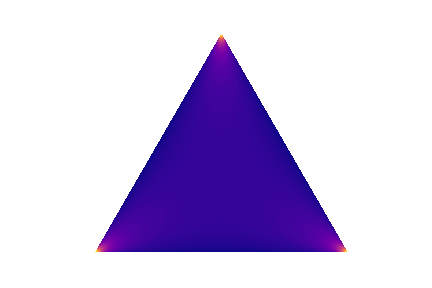
\includegraphics[width=\textwidth]{plots/notebooks/gs1.png}
\subcaption{}
\end{minipage}
\hfill
 \begin{minipage}[t]{.2\textwidth}
   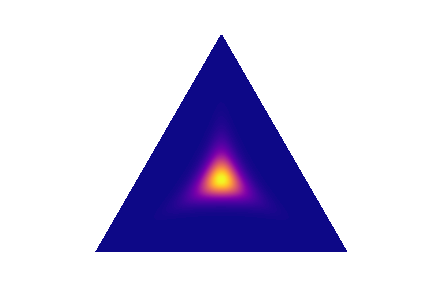
\includegraphics[width=\textwidth]{plots/notebooks/gs5.png}
\subcaption{}
\end{minipage}
\hfill
 \begin{minipage}[t]{.2\textwidth}
   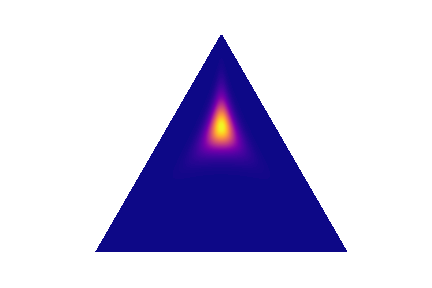
\includegraphics[width=\textwidth]{plots/notebooks/gs5_shift.png}
\subcaption{}
\end{minipage}

\caption{Пример распределения Gumbel-Softmax при различных значениях параметров: а)~$\lambda_{temp}\to0$, б)~$\lambda_{temp}=1, \mathbf{s}=[1,1,1]$, в)~$\lambda_{temp}=5, \mathbf{s}=[1,1,1]$, г)~$\lambda_{temp}=5, \mathbf{s}=[10,0.1,0.1].$}
\label{fig:gs}

\end{figure}


Заметим, что предлагаемое априорное распределение неоднозначно: одно и то же распределение  можно получить с различными значениями гиперпарамета $\mathbf{A}^{i,j}_k$ и структурного параметра $\gamma^{i,j}_k$. В качестве регуляризатора для матрицы $(\mathbf{A}^{i,j}_k)^{-1}$ предлагается использовать обратное гамма-распределение:
\[
    (\mathbf{A}^{i,j}_k)^{-1} \sim \text{inv-gamma}(\lambda_1,\lambda_2),
\]
где $\lambda_1,\lambda_2 \in \boldsymbol{\lambda}$ --- метапараметры оптимизации. 
Использование обратного гамма-распределения в качестве распределения гиперпараметров можно найти в~\cite{bishop,mackay}. В данной работе обратное распределение выступает как регуляризатор гиперпараметров.
Калибруя метапарамы   $\lambda_1,\lambda_2$ можно получить более сильную или более слабую регуляризацию~\cite{rvm}. Пример распределений $\text{inv-gamma}(\lambda_1,\lambda_2)$ для разных значений метапараметров $\lambda_1,\lambda_2$ изображен на Рис.~\ref{fig:inv-gamma}.

\begin{figure}
\centering
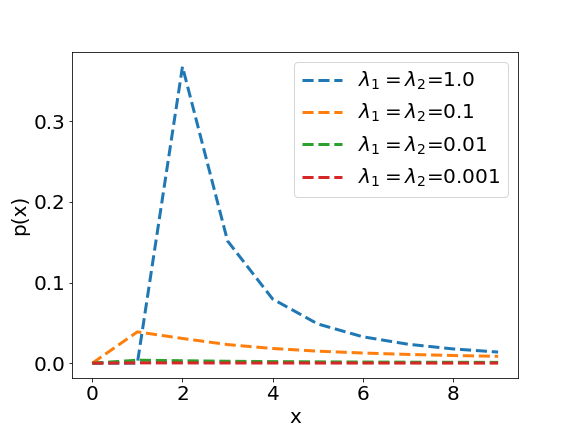
\includegraphics[width=0.6\textwidth]{plots/notebooks/invgamma.png}
\caption{Графики обратных гамма распределений для различных значений метапараметров.}
\label{fig:inv-gamma}
\end{figure}


Таким образом, предлагаемая вероятностная модель содержит следующие компоненты:
\begin{enumerate}
\item Параметры $\mathbf{w}$ модели, распределенные нормально.
\item Структура модели $\boldsymbol{\Gamma}$ распределены по распределению Gumbel-Softmax.
\item Гиперпараметры: $\mathbf{h} = [\text{diag}(\mathbf{A}), \mathbf{s}]$, где $\mathbf{A}$ --- конкатенация матриц $\mathbf{A}^{j,k}, (j,k) \in E,$ $\mathbf{s}$ --- конкатенация параметров Gumbel-Softmax распределений $\mathbf{s}^{j,k}, (j,k) \in E$, где $E$ --- множество ребер, соответствующих графу рассматриваемого параметрического семейства.
\item Метапараметры: $\boldsymbol{\lambda} = [\lambda_1, \lambda_2].$
\end{enumerate}

График вероятностной модели в формате плоских нотаций представлен на Рис.~\ref{fig:plate_prob}.
\begin{figure}
\centering
   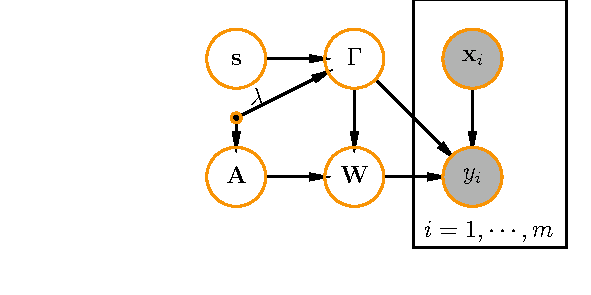
\includegraphics[width=0.5\textwidth]{plots/notebooks/simple_plate.pdf}
\caption{График предлагаемой вероятностной модели в формате плоских нотаций. Переменные обозначены белыми и серыми кругами, константы обозначены обведенными черными кругами. Наблюдаемые переменные обозначены серыми кругами.}
\label{fig:plate_prob}
\end{figure}

\section{Вариационная оценка для обоснованности вероятностной модели}
В качестве критерия выбора структуры модели предлагается использовать апостериорную вероятность гиперпараметров:
\begin{equation}
\label{eq:optimal_hyper}
    p(\mathbf{h}|\mathbf{y}, \mathbf{X}, \boldsymbol{\lambda}) \propto p(\mathbf{y}|\mathbf{X}, \mathbf{h}, \boldsymbol{\lambda}) p(\mathbf{h}|\boldsymbol{\lambda}) \to \max_{\mathbf{h} \in \mathbb{H}},
\end{equation}
где структура модели и параметры модели выбираются на основе полученных значений гиперпараметров:
\[
    \boldsymbol{\Gamma}^* = \argmax_{\boldsymbol{\Gamma} \in \amsmathbb{\Gamma}} p(\boldsymbol{\Gamma}|\mathbf{y}, \mathbf{X}, \mathbf{h}^*),
\]
\[
    \mathbf{w}^* = \argmax_{\mathbf{w} \in \mathbb{W}} p(\mathbf{w}|\mathbf{y}, \mathbf{X}, \boldsymbol{\Gamma}^*, \mathbf{h}^*),
\]
где $\mathbf{h}^*$ --- решение задачи оптимизации~\eqref{eq:optimal_hyper}.

Для вычисления обоснованности $$p(\mathbf{y}|\mathbf{X}, \mathbf{h}, \boldsymbol{\lambda}) = \iint_{\boldsymbol{\Gamma},\mathbf{w}}p(\mathbf{y}|\mathbf{X}, \mathbf{w}, \boldsymbol{\Gamma},\boldsymbol{\lambda})p(\mathbf{w}|\boldsymbol{\Gamma},\mathbf{h}, \boldsymbol{\lambda})p(\boldsymbol{\Gamma}|\mathbf{h}, \boldsymbol{\lambda})d\boldsymbol{\Gamma}d\mathbf{w}$$ из~\eqref{eq:optimal_hyper} предлагается использовать вариационную оценку обоснованности.

\begin{theorem}
Пусть $q(\mathbf{w},\boldsymbol{\Gamma}|\boldsymbol{\theta})  = q(\mathbf{w},\boldsymbol{\Gamma}|\boldsymbol{\theta}_\mathbf{w})q_{\boldsymbol{\Gamma}}(\boldsymbol{\Gamma}|\boldsymbol{\theta}_{\boldsymbol{\Gamma}})$ --- вариационное распределение c параметрами $\boldsymbol{\theta}= [\boldsymbol{\theta}_\mathbf{w},\boldsymbol{\theta}_{\boldsymbol{\Gamma}} ]$, аппроксимирующее апостериорное распределение структуры и параметров:
\[
    q(\mathbf{w},\boldsymbol{\Gamma}|\boldsymbol{\theta}) \approx p(\mathbf{w},\boldsymbol{\Gamma}|\mathbf{y}, \mathbf{X}, \mathbf{h}, \boldsymbol{\lambda}),
\]
\[
    q_{\mathbf{w}}(\mathbf{w}|\boldsymbol{\theta}_\mathbf{w},\boldsymbol{\Gamma}) \approx p(\mathbf{w}|\mathbf{y}, \mathbf{X},  \boldsymbol{\Gamma},\mathbf{h}, \boldsymbol{\lambda}),
\]
\[
    q_{\boldsymbol{\Gamma}}(\boldsymbol{\Gamma}|\boldsymbol{\theta}_{\boldsymbol{\Gamma}}) \approx p(\boldsymbol{\Gamma}|\mathbf{y}, \mathbf{X},  \mathbf{h}, \boldsymbol{\lambda}).
\]

Тогда справедлива следующая оценка:
\begin{equation}
\label{eq:full_elbo}
\text{log} p(\mathbf{y}|\mathbf{X}, \mathbf{h}, \boldsymbol{\lambda}) \geq
\end{equation}
\[
 \mathsf{E}_{\boldsymbol{\Gamma} \sim q_{\boldsymbol{\Gamma}}}\mathsf{E}_{\mathbf{w} \sim q_{\mathbf{w}}} \text{log}p(\mathbf{y}|\mathbf{w}, \boldsymbol{\Gamma}, \mathbf{X}) - D_\text{KL}\left(q_{\boldsymbol{\Gamma}}(\boldsymbol{\Gamma}|\boldsymbol{\theta}_{\boldsymbol{\Gamma}})|p(\boldsymbol{\Gamma}|\mathbf{h}, \boldsymbol{\lambda})\right) - D_\text{KL}\left(q_{\mathbf{w}}(\mathbf{w}|\boldsymbol{\theta}_\mathbf{w},\boldsymbol{\Gamma})|p(\mathbf{w}|\boldsymbol{\Gamma}, \mathbf{h})\right),
\]
где $D_\text{KL}\left(q_{\mathbf{w}}(\mathbf{w}|\boldsymbol{\theta}_\mathbf{w},\boldsymbol{\Gamma})|p(\mathbf{w}|\boldsymbol{\Gamma}, \mathbf{h})\right)$ вычисляется по формуле условной дивергенции~\cite{TODO}:
\[
D_\text{KL}\left(q_{\mathbf{w}}(\mathbf{w}|\boldsymbol{\theta}_\mathbf{w},\boldsymbol{\Gamma})|p(\mathbf{w}|\boldsymbol{\Gamma}, \mathbf{h})\right) = \mathsf{E}_{\boldsymbol{\Gamma} \sim q_{\boldsymbol{\Gamma}}} \mathsf{E}_{\mathbf{w} \sim q_{\mathbf{w}}} \frac{\text{log}q(\mathbf{w}|\boldsymbol{\Gamma})}{\text{log}p(\mathbf{w}|\mathbf{h},\boldsymbol{\Gamma})}.
\]
\end{theorem}

\begin{proof}
Используя неравенство Йенсена получим 
\[
\text{log} p(\mathbf{y}|\mathbf{X}, \mathbf{h}, \boldsymbol{\lambda}) \geq
\]
\[
   \mathsf{E}_{q} \text{log}p(\mathbf{y}|\mathbf{w}, \boldsymbol{\Gamma}, \mathbf{X}) - D_\text{KL}(q (\mathbf{w},\boldsymbol{\Gamma}|\boldsymbol{\theta})|p(\mathbf{w},\boldsymbol{\Gamma}|\mathbf{h})).
\]

Декомпозируем распределение $q$ по свойству условной дивергенции:
\[
D_\text{KL}(q (\mathbf{w},\boldsymbol{\Gamma}|\boldsymbol{\theta})|p(\mathbf{w},\boldsymbol{\Gamma}|\mathbf{h})) = D_\text{KL}\left(q_{\boldsymbol{\Gamma}}(\boldsymbol{\Gamma}|\boldsymbol{\theta}_{\boldsymbol{\Gamma}})|p(\boldsymbol{\Gamma}|\mathbf{h}, \boldsymbol{\lambda})\right) + D_\text{KL}\left(q_{\mathbf{w}}(\mathbf{w}|\boldsymbol{\theta}_\mathbf{w},\boldsymbol{\Gamma})|p(\mathbf{w}|\boldsymbol{\Gamma}, \mathbf{h})\right).    
\]
\end{proof}

В качестве вариационного распределения $q_{\mathbf{w}}$ предлагается использовать нормальное распределение, не зависящее от структуры модели $\boldsymbol{\Gamma}$:
\[
    q_{\mathbf{w}} = \mathcal{N}(\boldsymbol{\mu}, \mathbf{A}_q), 
\]
где $\mathbf{A}_q$ --- диагональная матрица с диагональю $\boldsymbol{\alpha}_q$.

В качестве вариационного распределения $q_{\boldsymbol{\Gamma}}$ предлагается использовать произведение распределений Gumbel-Softmax. Конкатенацию параметров концентрации распределений обозначим $\mathbf{s}_q$. Его температуру обозначим $\theta_\text{temp}$.

Вариационными параметрами распределения $q$ являются параметры распределений $q_{\mathbf{w}}, q_{\boldsymbol{\Gamma}}$:
\[
    \boldsymbol{\theta} = [\boldsymbol{\mu}, \boldsymbol{\alpha}_q, \mathbf{s}_q, \theta_\text{temp}]. 
\]


График вероятностной вариационной модели в формате плоских нотаций представлен на Рис.~\ref{fig:plate_qprob}.
\begin{figure}
\centering
   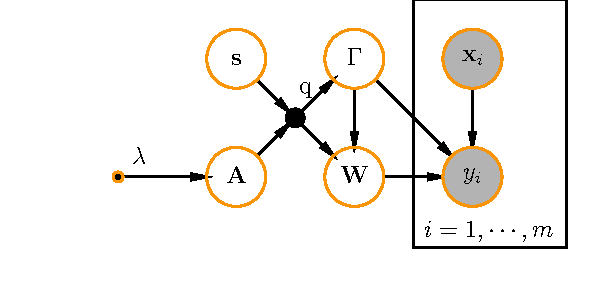
\includegraphics[width=0.5\textwidth]{plots/notebooks/plate.pdf}
\caption{График предлагаемой вероятностной вариационной модели в формате плоских нотаций. Переменные обозначены белыми и серыми кругами, константы обозначены обведенными черными кругами. Вариационное распределение обозначено черным кругом. Наблюдаемые переменные обозначены серыми кругами.}
\label{fig:plate_qprob}
\end{figure}

Для анализа сложности полученной модели введем понятие \textit{параметрической сложности}. 
\begin{defin} 
Параметрической сложностью  $C_p(\boldsymbol{\theta})$ модели с вариационными параметрами $\boldsymbol{\theta}$ на компакте $U_\mathbf{h} \subset \mathbb{H}$ назовем минимальную дивергенцию между вариационным и априорным распределением:
\[
C_p(\boldsymbol{\theta}|U_\mathbf{h}) = \min_{\mathbf{h} \in U_\mathbf{h}} \text{D}_\text{KL}\left(q(\mathbf{w}, \boldsymbol{\Gamma}|\boldsymbol{\theta})|p(\mathbf{w}, \boldsymbol{\Gamma}|\mathbf{h})\right).
\]
\end{defin}
Параметрическая сложность модели соответствует ожидаемой длине описания параметров модели при условии заданного параметрического априорного распределения~\cite{hinton_mdl}.

Одним из критериев удаления неинформативных параметров в вероятностных моделях является отношение вариационной плотности параметров в моде распределения к вариационной плотности параметра в нуле~\cite{nips}:
\[
    \frac{q_\mathbf{w}(\mu|\boldsymbol{\theta}_\mathbf{w})}{q(0|\boldsymbol{\theta}_\mathbf{w})} = \text{exp}\left(-\frac{2\alpha_q^2}{\mu^2}\right),
\]
где $q_\mathbf{w}(w|\boldsymbol{\theta}_\mathbf{w}) \sim \mathcal{N}(\mu, \alpha_q).$

Обобщим понятие относительной вариационной плотности на случай произвольных распределений.
\begin{defin}
Относительной вариационной   плотностью параметра $w \in \mathbf{w}$  при условии структуры $\boldsymbol{\Gamma}$ и гиперпараметров $\mathbf{h}$ назовем отношение моды вариационного распределения параметра к моде априорного распределению параметра:
\[
    \rho(w|\boldsymbol{\Gamma}, \boldsymbol{\theta}_\mathbf{w}, \mathbf{h},\boldsymbol{\lambda}) = \frac{q\bigl(\text{mode}~q\left(w|\boldsymbol{\Gamma}, \boldsymbol{\theta}_\mathbf{w}\right)|\boldsymbol{\Gamma}, \boldsymbol{\theta}_\mathbf{w}\bigr)}{q\bigl(\text{mode}~p\left({w}|\boldsymbol{\Gamma}, \mathbf{h},\boldsymbol{\lambda}\right)|\boldsymbol{\Gamma},\boldsymbol{\theta}_\mathbf{w}\bigr)},
\]
\[
    \boldsymbol{\rho}(\mathbf{w}|\boldsymbol{\Gamma}, \boldsymbol{\theta}_\mathbf{w}, \mathbf{h},\boldsymbol{\lambda}) = \prod_{w \in \mathbf{w}}\rho(w|\boldsymbol{\Gamma}, \boldsymbol{\theta}_\mathbf{w}, \mathbf{h},\boldsymbol{\lambda}).
\]

\end{defin}

Сформулируем и докажеми теорему о связи относительной плотности и параметрической сложности модели:

\begin{theorem}
Пусть
\begin{enumerate}
\item заданы компактные множества $U_\mathbf{h} \subset \mathbb{H}, U_{\boldsymbol{\theta}} \subset \amsmathbb{\Theta}$;


\item мода априорного распределения $p(\mathbf{w},\boldsymbol{\Gamma}| \mathbf{h}))$ не зависит от гиперпараметров $\mathbf{h}$ на $U_\mathbf{h}$:
\[
    p(\mathbf{w},\boldsymbol{\Gamma}| \mathbf{h}_1) = p(\mathbf{w},\boldsymbol{\Gamma}| \mathbf{h}_2) =  p(\mathbf{w},\boldsymbol{\Gamma}) \forall \mathbf{h}_1,\mathbf{h}_2 \in U_{\mathbf{h}}. 
\]

\item вариационное распределение $q_\mathbf{w}$ и априорное распределение $p(\mathbf{w},\boldsymbol{\Gamma}| \mathbf{h}))$  являются абсолютно непрерывными и унимодальными на  $U_\mathbf{h} \subset \mathbb{H}, U_{\boldsymbol{\theta}}$.

\item мода и матожидание вариационного распределение $q$ и априорного распределение $p(\mathbf{w},\boldsymbol{\Gamma}| \mathbf{h}))$  распределения совпадают.

\item задана последовательность $\boldsymbol{\theta}_1,\boldsymbol{\theta}_2,\dots$ --- бесконечная последовательность векторов вариационных параметров, такая что $\lim_{i \to \infty}C_p(\boldsymbol{\theta_i}|U_{\mathbf{h}}) = 0, \boldsymbol{\theta} \in U_{\boldsymbol{\theta}}.$ 

\item $\mathbf{h}_i$. 
\end{enumerate}
$\mathbf{h}_i$.
Тогда матожидание вариационной плотности данной последовательности стремится к единице:
\[
   \mathsf{E}_q \boldsymbol{\rho}(\mathbf{w}|\boldsymbol{\Gamma}, \boldsymbol{\theta}_\mathbf{w}, \mathbf{h},\boldsymbol{\lambda})^{-1} \to 1.
\]


\end{theorem}

\begin{proof}
Воспользуемся неравенством Пинскера:
\[
    ||F_q(\boldsymbol{\theta}) - F_p(\mathbf{h})||_\text{TV},\leq\sqrt{2\text{D}_\text{KL}\left(q(\mathbf{w}, \boldsymbol{\Gamma}|\boldsymbol{\theta})|p(\mathbf{w}, \boldsymbol{\Gamma}|\mathbf{h})\right)},
\]
где $|\cdot|_\text{TV}$ --- расстояние по вариации, $F_q, F_p$ --- функции распределения   $q(\mathbf{w},\boldsymbol{\Gamma}|\boldsymbol{\theta})$ и $p(\mathbf{w},\boldsymbol{\Gamma}| \mathbf{h}, \boldsymbol{\lambda})$.
Отсюда $ \lim_{i \to \infty} ||F_q(\boldsymbol{\theta}) - F_p(\mathbf{h})||_\text{TV} = 0.$
Из сходимости по вариации следует слабая сходимость распределений.

Рассмотрим разность мод:
\[
\mathsf{E}_{q_{\boldsymbol{\Gamma}}}\text{mode}~q_{\mathbf{w}}(\mathbf{w}|\boldsymbol{\theta}_\mathbf{w},\boldsymbol{\Gamma}) - \mathsf{E}_{p(\boldsymbol{\Gamma}|\mathbf{h}, \boldsymbol{\lambda})} \text{mode}~p(\mathbf{w}|\boldsymbol{\Gamma}, \mathbf{h}) =
\]
\[
= \mathsf{E}_{q}\mathbf{w} - \mathsf{E}_{p(\mathbf{w},\boldsymbol{\Gamma}|\mathbf{h})}\mathbf{w}.
\]

Т.к. вторые моменты величины $\mathbf{w}$ конечны для вариационного и априорного распределения, то функции $\mathsf{E}_{q(\mathbf{w}|\boldsymbol{\theta}_\mathbf{w},\boldsymbol{\Gamma})}\mathbf{w}, \mathsf{E}_{p(\mathbf{w},\boldsymbol{\Gamma}| \mathbf{h})}$ абсолютно интегрируемы, что в сочетании со слабой сходимостью позволяет записать:
\[
  \lim_{i \to \infty}\bigl( \mathsf{E}_{q}\mathbf{w} -  \mathsf{E}_{p(\mathbf{w},\boldsymbol{\Gamma}|\mathbf{h})}\mathbf{w} \bigr) = 0.
\]
Таким образом в пределе моды вариационного распределения $q(\mathbf{w},\boldsymbol{\Gamma}|\boldsymbol{\theta})$ и априорного распределения $p(\mathbf{w},\boldsymbol{\Gamma}| \mathbf{h})$ совпадают.
%http://www.math.chalmers.se/~serik/WeakConv/C-space.pdf
%https://math.stackexchange.com/questions/2923/do-convergence-in-distribution-along-with-uniform-integrability-imply-convergenc
% https://web.ma.utexas.edu/users/gordanz/notes/uniform_integrability.pdf   
%file:///home/legin/%D0%97%D0%B0%D0%B3%D1%80%D1%83%D0%B7%D0%BA%D0%B8/weak_convergence.pdf
Т.к. наибольшее значение распределения $q$ сосредоточено в моде распределения $q$, то $\boldsymbol{\rho}(\mathbf{w}|\boldsymbol{\Gamma}, \boldsymbol{\theta}_\mathbf{w}, \mathbf{h},\boldsymbol{\lambda})^{-1}$ ограничена сверху единицей. Рассмотрим матожидание функции, обратной к отношению вариационных плотностей:
\[
\mathsf{E}_q \boldsymbol{\rho}(\mathbf{w}|\boldsymbol{\Gamma}, \boldsymbol{\theta}_\mathbf{w}, \mathbf{h},\boldsymbol{\lambda})^{-1}
\] 
Т.к. функция ограничена, то предел можно внести под знак интеграла:
\[
\lim_{i \to \infty} \mathsf{E}_q \boldsymbol{\rho}(\mathbf{w}|\boldsymbol{\Gamma}, \boldsymbol{\theta}_\mathbf{w}, \mathbf{h},\boldsymbol{\lambda})^{-1} = 
\]
\[
 =\mathsf{E}_q  \lim_{i \to \infty}  \boldsymbol{\rho}(\mathbf{w}|\boldsymbol{\Gamma}, \boldsymbol{\theta}_\mathbf{w}, \mathbf{h},\boldsymbol{\lambda})^{-1} = 1.
\]

\end{proof}

Теорема утверждает, что при устремлении параметрической сложности модели к нулю, параметры модели станоятся неинформативными и подлежащими удалению в среднем по всем возможным значениям  структуры  $\boldsymbol{\Gamma}$ модели. Заметим, что теорема применима для случая, когда последовательность вариационных распределений $q$ не имеет предела. Так, в случае, если структура $\boldsymbol{\Gamma}$ определена однозначно, последовательность $q_i$ может являться последовательностью нормальных расп распределений, чье матожидание стремится к нулю. Априорным распределением $p(\mathbf{w},\boldsymbol{\Gamma}|\mathbf{h}) = p(\mathbf{w}|\mathbf{h})$ при этом может являться семейство нормальных распределений с нулевым средним.

\section{Обобщающая задача}
Рассмотрим основные критерии выбора вероятностных моделей.

\begin{enumerate}
\item Критерий максимального правдоподобия:
\[
    \text{log}p(\mathbf{y}|\mathbf{X}, \mathbf{w}) \to \max_{\mathbf{w} \in \mathbb{W}}.
\]

Метод заключается в максимизации правдоподобия обучающей выборки и подвержен переобучению.
Для использования данного метода в качестве задачи выбора модели предлагается следующее обобщение:
\begin{equation}
\label{eq:optim_ml}
    L =  \mathsf{E}_q \text{log} \text{log}p(\mathbf{y}|\mathbf{X}, \mathbf{w}).
\end{equation}
Данное обобщение эквивалентно  методу правдоподобия при выборе в качестве $q$ эмпирического распределения парамтетров и структуры.
Метод не предполагает оптимизации гиперпараметров. Для формального соответствия данной задачи задаче выбора положим $L=Q$.


\item Метод максимальной апостериорной вероятности. 
\[
    \text{log}p(\mathbf{y},\mathbf{w}|\mathbf{X}, \mathbf{h} ) \to \max_{\mathbf{w} \in \mathbb{W}}.
\]
Аналогично предыдущему методу сформулируем вариационное обобщение данной задачи:
\begin{equation}
\label{eq:optim_map}
    L = Q = \mathsf{E}_q \text{log} \text{log}p(\mathbf{y}|\mathbf{X}, \mathbf{w})+\text{log}p(\mathbf{w}|\boldsymbol{\lambda}) + \text{log}p(\boldsymbol{\gamma}|\mathbf{X}, \mathbf{w}).
\end{equation}
В рамках данной задачи оптимизации параметры априорных распределений $\mathbf{A}, \mathbf{s}$ выступают в качестве метапараметров и не подлежат оптимизации.



\item Перебор структуры:
\begin{equation}
\label{eq:optim_struct}
    L =  Q = \mathsf{E}_q\text{log}p(\mathbf{y}, \mathbf{w}|\mathbf{X})[q_{\boldsymbol{\Gamma}} = p']
\end{equation}
где $p'$ --- некоторое распределение на структуре, выступающее в качестве метапараметра.




\item Критерий Акаике:
\[
   Q =  \text{log}p(\mathbf{y}|\mathbf{X}, \mathbf{w}) - |\mathbb{W}|.
\]
Заметим,что в условия выбора модели на параметрическом множестве моделей данный критерий не имеет смысла, т.к. количество параметров для каждой модели одинаково. Предлагается следующая переформулировка:
\begin{equation}
\label{eq:optim_aic}
    L = Q = \text{log}p(\mathbf{y}|\mathbf{X}, \mathbf{w}) - |\{w: C_p(\theta|U_\mathbf{h})<\lambda\}|,
\end{equation}
где $\lambda$ --- метапараметр алгоритма, $U_\mathbf{h}  \subset \mathbb{H}$ --- область определения задачи по гиперпараметрам.

\item Информационный критерий Шварца:
\[
    \text{log}p(\mathbf{y}|\mathbf{X}, \mathbf{w}) - 0.5\text{log}(m)|\{w: C_p(\theta|U_\mathbf{h})<\lambda\}|.
\]
Переформулируем данный критерий аналогично критерию AIC:
\begin{equation}
\label{eq:optim_bic}
    L = Q = BIC_{\lambda} = \text{log}p(\mathbf{y}|\mathbf{X}, \mathbf{w}) - \text{log}(m)|\{w: C_p(w)<\lambda\}|.
\end{equation}


\item Метод вариационной оценки обоснованности.
\begin{equation}
\label{eq:optim_elbo_method}
    L = Q = \mathsf{E}_q \text{log}p(\mathbf{y}|\mathbf{X}, \mathbf{w}) - D_\text{KL}(q|p).
\end{equation}


\item Hold-out кросс-валидация.
\begin{equation}
\label{eq:optim_hold_out}
    L = \mathsf{E}_q \text{log}p(\mathbf{y}, \mathbf{w}|\mathbf{X}, \mathbf{h}),
\end{equation}
\[
    Q = \mathsf{E}_q \text{log}p(\mathbf{y}|\mathbf{X}, \mathbf{w}).
\]


\end{enumerate}

Каждый из рассмотренных критерии удовлетворяет хотя бы одному из перечисленных свойтсв:
\begin{enumerate}
\item Модель, оптимизируемая согласно критерию, доставляет максимум правдоподобия выборки;
\item Модель, оптимизируемая согласно критерию, доставляет максимум оценки обоснованности;
\item Для моделей, доставляющих сопоставимые значения правдоподобия выборки, выбирается модель с меньшим количеством информативных параметров.
\item Критерий позволяет производить перебор структур для отбора наилучших модели.
\end{enumerate}

Формализуем рассмотренные критерии. Оптимизационную задачу, которая удовлетворяет всем перечисленным свойствам, будет называть \textit{обобщающей}.

\begin{defin}
Двухуровневую задачу оптимизации будем называть \textit{обобщающей} на области $U \subset \amsmathbb{\Theta} \times \mathbb{H} \times \amsmathbb{\Lambda}$, если она удовлетворяет следующим свойствам:
\begin{enumerate}
\item Для каждого значения гиперпараметров $\mathbf{h}$ оптимальное решение нижней задачи оптимизации $\boldsymbol{\theta}^{*}$ определено однозначно.

\item Свойство максимизации правдоподобия выборки: существует $\boldsymbol{\lambda} \in U_{\lambda}$ и  $K_1 \in \mathbb{R}_{+}$, такие что для любых векторов гиперпараметров, удовлетворяющих неравенству $\mathbf{h}_1, \mathbf{h}_2 \in  U_{h}, Q(\mathbf{h}_1) - Q(\mathbf{h}_2) > K_1$, выполняется неравенство $\mathsf{E}_q \text{log}~p(\mathbf{y}|\mathbf{X}, \boldsymbol{\theta}_1, \lambda_{\text{temp}}, \mathbf{f})>\text{log}\mathsf{E}_q ~p(\mathbf{y}|\mathbf{X}, \boldsymbol{\theta}_2, \lambda_{\text{temp}}, \mathbf{f})$.

\item Свойство минимизации параметрической сложности:  существует  $\boldsymbol{\lambda} \in U_{\lambda}$ и $K_2 \in \mathbb{R}_{+}$, такие что для любых векторов гиперпараметров $\mathbf{h}_1, \mathbf{h}_2 \in U_h$, удовлетворяющих неравенству $Q(\mathbf{h}_1) - Q(\mathbf{h}_2) > K_2$ и при этом имеющие равенство ожидаемых правдоподобий выборок  $\mathsf{E}_q \text{log}~p(\mathbf{y}|\boldsymbol{\theta}_1, \lambda_{\text{temp}}, \mathbf{f}) = \text{log}\mathsf{E}_q ~p(\mathbf{y}|\boldsymbol{\theta}_2, \lambda_{\text{temp}}, \mathbf{f})$, параметрическая сложность первой модели меньше, чем второй: $C_p(\boldsymbol{\theta}^{*}(\mathbf{h}_1)|U_\mathbf{h})<C_p(\boldsymbol{\theta}^{*}(\mathbf{h}_2|U_\mathbf{h})$.

\item Свойства приближения оценки обоснованности: существует значение гиперпараметров $\boldsymbol{\lambda}$, такое что оптимизация задачи эквивалента оптимизации вариационной оценки обоснованности модели: $\argmax_{\mathbf{h} \in U_h}Q(\argmax_{\boldsymbol{\theta}} \in U_{\boldsymbol{\theta}} L) \approx \argmax_{\mathbf{h} \in U_h} \mathsf{E}_q p(\mathbf{y}|\mathbf{w}, \mathbf{X}) - {D}_{KL}(q|p).$

\item Свйоство перебора структур: существует константа $K_3$, такая что для любых двух векторов $\mathbf{h}_{1}, \mathbf{h}_2$ и соответствующих векторов $\boldsymbol{\theta}_1^{*},\boldsymbol{\theta}_2^{*}: D_\text{KL}(q_{\boldsymbol{\Gamma}_2}, q_{\boldsymbol{\Gamma}_1})>K_3, D_\text{KL}(q_{\boldsymbol{\Gamma}_1}, q_{\boldsymbol{\Gamma}_2})>K_3$  существуют значения гиперпараметров $\boldsymbol{\lambda_1},\boldsymbol{\lambda_2}$, такие что  $Q(\mathbf{h}_1, \lambda_1) > Q(\mathbf{h}_2, \lambda_1), Q(\mathbf{h}_1, \lambda_1) < Q(\mathbf{h}_2, \lambda_2)$.

\item Свойство нерперывности: $\mathbf{h}^{*}, \boldsymbol{\theta}^{*}$ непрерывны по метапараметрам.
\end{enumerate}
\end{defin}
Первое свойство говорит о том, что решение первого и второго уровня должны быть согласованы и определены однозначно.
Свойства 2-4 определяют возможные критерии оптимизации, которые должны приближаться обобщающей задачей.
Свойство 5 говорит о возможности перехода между различными структурами модели. Отметим, что данное условие крайне важно в условиях оптимизации моделей глубокого обучения, которые отличаются многоэкстремальностью.
Последнее свойство говорит о том, что обобщающая задача должна позволять производить переход между различными критериями выбора  параметров и структуры модели непрерывно.

\begin{theorem}Рассмотренные задачи~\eqref{eq:optim_ml},\eqref{eq:optim_map},\eqref{eq:optim_struct},\eqref{eq:optim_aic},\eqref{eq:optim_bic},\eqref{eq:optim_elbo_method},\eqref{eq:optim_hold_out} не являются обобщающими.
\end{theorem}
\begin{proof}
TODO
\end{proof}

\begin{theorem}
Пусть задано непустое множество непрерывных по параметрам распределний на структуре $\mathbf{P}$. 
Пусть функции потерь и валидации $L,Q$ являются непрерывно-дифференцируемыми на компакте $U\subset \amsmathbb{\Theta} \times \mathbb{H} \times \amsmathbb{\Lambda}$, где параметры распределений $\mathbf{P} \in \amsmathbb{\Lambda}.$ 
Тогда следующая задача является обобщающей на $U$.
\begin{equation}
\tag{$Q^{*}$}
\label{eq:qopt}
\mathbf{h}^{*} = \argmax_{\mathbf{h}} Q = 
\end{equation}
\[
= {\lambda_\text{likelihood}^\text{Q}\mathsf{E}_{{q}^{*}} \text{log}~{p(\mathbf{y} | \mathbf{X}, \mathbf{w},\boldsymbol{\Gamma}, \mathbf{h}, \lambda_\text{temp}, \mathbf{f})}}
 -\]
\vspace{-0.3cm}
\[- {\lambda^\text{prior}_\text{Q}\text{D}_{KL}\bigl( q^{*}(\mathbf{w}, \boldsymbol{\Gamma}) || p(\mathbf{w}, \boldsymbol{\Gamma} |\mathbf{h}, \lambda_{\text{temp}},\mathbf{f}) \bigr)}  -\]
\vspace{-0.3cm}
\[
 - {\sum_{p' \in \mathbf{P}, \lambda \in \boldsymbol{\lambda}^\text{struct}_\text{Q}} \lambda\text{D}_{KL}(\boldsymbol{\Gamma} | p') + \text{log}p(\mathbf{h}|\mathbf{f})}, 
\]
где 
\begin{equation}
\tag{$L^{*}$}
{q}^{*} = \argmax_{q} L = 
{\mathsf{E}_q \text{log}~{p(\mathbf{y} | \mathbf{X}, \mathbf{w}, \boldsymbol{\Gamma}, \mathbf{h}, \lambda_{\text{temp}}, \mathbf{f})}}
\end{equation}
\vspace{-0.3cm}
\[- {\lambda^\text{prior}_\text{L}\text{D}_{KL}\bigl( q^{*}(\mathbf{w}, \boldsymbol{\Gamma}) || p(\mathbf{w}, \boldsymbol{\Gamma} |\mathbf{h}, \lambda_{\text{temp}},\mathbf{f}) \bigr)}.
\]
\end{theorem}
\begin{proof}
Для доказательста теоремы требуется доказать критерии 1-6 из определения обобщающей задачи.
Критерий 1 следует из условий задачи.

Докажем критерий 2. Пусть $\lambda^\text{prior}_\text{Q} = 0, \boldsymbol{\lambda}^\text{struct}_\text{Q} = \mathbf{0}$. Зафиксируем некоторое значение метапараметров $\lambda_1, \lambda_2$. Т.к. $U_\mathbf{h}$ --- компакт, возьмем в качестве константы $K_1$ разницу между максимальным и минимальным значением $p(\mathbf{h}|\mathbf{f})$:
\[
    K = \max_{\mathbf{h}} \text{log}~p (\mathbf{h}|\mathbf{f}) - \min_{\mathbf{h}} \text{log}~p(\mathbf{h}|\mathbf{f}).
\]
Тогда $Q(\mathbf{h}_1) - Q(\mathbf{h}_2) = \mathsf{E}_q \text{log}~p(\mathbf{y}|\mathbf{X}, \boldsymbol{\theta}_1 \lambda_{\text{temp}}, \mathbf{f}) - \mathsf{E}_q \text{log}~p(\mathbf{y}|\mathbf{X}, \boldsymbol{\theta}_2, \lambda_{\text{temp}}, \mathbf{f}) + \text{log}~p(\mathbf{h}_2|\mathbf{f}) - \text{log}~p(\mathbf{h}_1|\mathbf{f})>K_1.$ Отсюда следует $\mathsf{E}_q \text{log}~p(\mathbf{y}|\mathbf{X}, \boldsymbol{\theta}_1 \lambda_{\text{temp}}, \mathbf{f}) > \mathsf{E}_q \text{log}~p(\mathbf{y}|\mathbf{X}, \boldsymbol{\theta}_2 \lambda_{\text{temp}}, \mathbf{f}).$

Докажем критерий 3.  Пусть $\lambda^\text{likelihood}_\text{Q} = 0, \boldsymbol{\lambda}^\text{struct}_\text{Q} = \mathbf{0}$. Зафиксируем некоторое значение метапараметров $\lambda_1, \lambda_2$. Т.к. $U_\mathbf{h}$ --- компакт, возьмем в качестве константы $K_1$ разницу между максимальным и минимальным значением $p(\mathbf{h}|\mathbf{f})$:
TODO

Докажем критерий 4. Пусть $\lambda^\text{likelihood}_\text{Q} = \lambda^\text{prior}_\text{Q}=\lambda^\text{prior}_\text{L}=1, \boldsymbol{\lambda}^\text{struct}_\text{Q} = \mathbf{0}$. Тогда оптимизационную задачу можно записать как: TODO, что и требовалось доказать.

Докажем критерий 5. TODO

Докажем критерий 6. TODO
\end{proof}

Метапараметрами данной задачи являются коэффициенты $\lambda^\text{prior}_\text{Q}, \lambda^\text{prior}_\text{L}$, отвечающие за регуляризацию верхней и нижней задачи оптимизации, коэффициент $\lambda_\text{likelihood}^\text{Q}$ за максимизацию правдоподобия, а также параметры распрделений $\mathbf{P}$ и вектор коэффициентов перед ними $\boldsymbol{\lambda}^\text{struct}_\text{Q}$. 

В предельном случае, когда множество температура $\lambda_\text{temp}$ близка к нулю, а множество $\mathbf{P}$ состоит из распределений, близких к дискретным, и соответствующих всем возможным структурам, калибровка $\boldsymbol{\lambda}^\text{struct}_\text{Q}$ порождает последовательность задач оптимизаций, схожую с перебором структур.  Для примера рассмотрим вырожденный случай поведения функции $Q$, когда $\lambda_\text{likelihood}^\text{Q} = \lambda^\text{prior}_\text{Q} = 0$. Пусть в Пусть модель использует один структурный параметр, в качестве априорного распределения на структуре задано распределение Gumbel-Softmax с $\lambda_\text{temp}=0.1$. Пусть в качестве множества распределений $\mathbf{P}$ используется два распределения Gumbel-Softmax, сконцентрированных близко к вершинам симплекса:
\[
    \mathbf{P} = [\text{Gumbel-Softmax}([0.8, 0.1, 0.1]^\text{T}, 0.1) ,\text{Gumbel-Softmax}([0.1, 0.8, 0.1]^\text{T}, 0.1)].
\]
Из определения распределения Gumbel-Softmax следует, что достаточно рассмотреть только значения параметра $\mathbf{s}$ находящиеся внутри симплекса.
На рис.~\ref{fig:gs_comb} изображены значения функции Q в зависимости от мета-параметров и значения гиперпараметра $\mathbf{s}$ распределения на структуре. Видно, что калибруя коэффициенты метапараметров получается последовательность оптимизаций, схожая с полным перебором структуры.


\textbf{Обобщающая задача: переформулировка через градиент}



Для вычисления приближенного значения функций $Q$ и $L$ предлагается использовать приближение методом Монте-Каарло с порождением $R$ реализаций величин $\mathbf{w}, \boldsymbol{\Gamma}$:

\[
   \mathsf{E}_q \text{log}~p(\mathbf{y}|\mathbf{X}, \boldsymbol{\theta}_1 \lambda_{\text{temp}}, \mathbf{f}) \approx   \sum_{r=1}^R \text{log}p(\mathbf{y}|\boldsymbol{\mu}+\boldsymbol{\alpha}_q \circ \hat{\epsilon}_r, \hat{\boldsymbol{\Gamma}}_r, \mathbf{X}).
\]
\[
D_\text{KL}\left(q_{\boldsymbol{\Gamma}}(\boldsymbol{\Gamma}|\boldsymbol{\theta}_{\boldsymbol{\Gamma}})|p(\boldsymbol{\Gamma}|\mathbf{h}, \boldsymbol{\lambda})\right)   \approx  \sum_{r=1}^R \left(\text{log}q_{\boldsymbol{\Gamma}}(\hat{\boldsymbol{\Gamma}}_r|\boldsymbol{\theta}_{\boldsymbol{\Gamma}})) - p(\hat{\boldsymbol{\Gamma}}|\mathbf{h},\boldsymbol{\lambda})\right),
\]
\[
D_\text{KL}\left(q_{\mathbf{w}}(\mathbf{w}|\boldsymbol{\theta}_\mathbf{w},\boldsymbol{\Gamma})|p(\mathbf{w}|\boldsymbol{\Gamma}, \mathbf{h})\right)  \approx  \sum_{(j,k) \in E}\sum_{l=1}^{K^{j,k}} D_\text{KL}\left(q_{\mathbf{w}}(\mathbf{w}^{j,k}_l|\boldsymbol{\theta}_\mathbf{w},\gamma^{j,k}_l)|p(\mathbf{w}^{j,k}_l|\gamma^{j,k}_l, \mathbf{h})\right)=
\]
\[ 
-\sum^{(j,k) \in E}\sum_{l=1}^{K_{j,k}} = \sum_{r=1}^R\frac{1}{2}\left( \left(\hat{\gamma}^{j,k}_r[l]\right)^{-1}\text{tr}((\mathbf{A}^{j,k}_l)_q(\mathbf{A}^{j,k}_l)^{-1}) + (\boldsymbol{\mu}^{j,k}_l)^{\mathsf{T}}\hat{\gamma}^{j,k}_r[l]^{-1}(\mathbf{A}^{j,k}_l)^{-1}\boldsymbol{\mu^{j,k}_l} - |\mathbf{w}^{j,k}_l| + \text{log}\frac{|\hat{\gamma}^{j,k}[l]_r\mathbf{A}^{j,k}_l|}{|(\mathbf{A}^{j,k}_l)_q|}\right),
\]
где $R$ --- количество реализаций случайных величин, по котором вычисляется значения вариационной оценки обоснованности, $\hat{\epsilon}_r \sim \mathcal{N}(0,1),$
 $\hat{\boldsymbol{\Gamma}}_r = [\boldsymbol{\gamma}^{j,k}_r, (j,k) \in E]$ --- реализация случайной величины, соответствующей структуре $\boldsymbol{\Gamma}$.

Для решения двухуровневой задачи предлагается использовать градиентные методы. 
\begin{theorem}
Пусть $Q,L$ --- локально выпуклы и непрерывны в некоторой области $U_{W} \times U_{\Gamma} \times U_H \times U_\lambda \subset \mathbb{W}\times\amsmathbb{\Gamma}\times\mathbb{H}\times\amsmathbb{\Lambda}$, при  этом $U_H \times U_\lambda$ --- компакт. 
Тогда решение задачи градиентной оптимизации стремится к локальному минимуму  $\mathbf{h}^{*} \in U$ исходной задачи оптимизации~\eqref{eq:qopt} при $\eta \to \infty$,
$\mathbf{h}^{*}$ является непрерывной функцией по метапараметрам модели.
\end{theorem}

\begin{proof}
TODO
\end{proof}

\section{Анализ обобщающей задачи}
В данном разделе рассматриваются свойства предложенной задачи при различных значениях метапараметров, а также характер ассимптотического поведения задач.

\begin{theorem}
Пусть задана выборка $\mathbf{X}, \mathbf{y}$ мощности $m$.\\
Пусть задана модель $\mathbf{f}(\mathbf{w}, \mathbf{X})$ и распределение $q$, апппроксимирующее апостериорное распределеине параметров $\mathbf{w}$ этой модели.\\
Рассмотрим выражение $\frac{1}{m} \text{ELBO}_{\gamma}$:\\
\[
    \frac{1}{m}\text{ELBO}_{\gamma}(\mathbf{X}, \mathbf{y}, q)= \frac{1}{m}\mathsf{E}_q \text{log}p(\mathbf{y}|\mathbf{X}, \mathbf{w}) - \frac{\gamma}{m}\text{KL}(q|p(\mathbf{w})),
\]
где $\gamma > 0$.

Пусть $\frac{1}{m} \text{ELBO}_{\gamma}$ сходится п.н. при $m \to \infty$ к функции $L(q)$\\ \textit{(вообще, она еще от гиперпараметров зависит, но здесь это будет лишним, прим. Олег).}

Тогда функция $\frac{1}{m_0} \text{ELBO}_{1}$ для  выборки мощности $m_0 = \frac{m}{\gamma}$ из той же генеральной совокупности сходится почти наверно к этой же функции $L(q)$:
\[
    \frac{1}{m_0} \text{ELBO}_{1}(\hat{\mathbf{X}}, \hat{\mathbf{y}}, q) \to^{\text{п.н.}} L(q),
\]
где $|\hat{\mathbf{X}}| = m_0$.
\end{theorem}
\begin{proof}
Рассмотрим величину  $\frac{1}{m}\text{ELBO}_{\gamma}$: \\
\[
    \frac{1}{m}\text{ELBO}_{\gamma}(\mathbf{X}, \mathbf{y})= \frac{1}{m}\mathsf{E}_q \text{log}p(\mathbf{y}|\mathbf{X}, \mathbf{w}) - \frac{\gamma}{m}\text{KL}(q|p(\mathbf{w})).
\]

По УЗБЧ: 
\[
    \frac{1}{m}\text{ELBO}_{\gamma}(\mathbf{X}, \mathbf{y}) \to_{m \to \infty}^{\text{п.н.}} \mathsf{E}_\mathbf{X}\mathsf{E}_{q} \text{log}p(\mathbf{y}|\mathbf{X}, \mathbf{w}) - \frac{\gamma}{m}\text{KL}(q|p(\mathbf{w})) = L(q).
\]

Аналогично рассмотрим $\frac{1}{m_0}\text{ELBO}_{1}$ для выборки мощностью $m_0 = \frac{m}{\gamma}$:
\[
    \frac{1}{m_0}\text{ELBO}_{1}(\hat{\mathbf{X}}, \hat{\mathbf{y}}) \to_{m \to \infty}^{\text{п.н.}} \mathsf{E}_\mathbf{X}\mathsf{E}_{q} \text{log}p(\mathbf{y}|\mathbf{X}, \mathbf{w}) - \frac{1}{m_0}\text{KL}(q|p(\mathbf{w})) = 
\]
\[
=  \mathsf{E}_\mathbf{X}\mathsf{E}_{q} \text{log}p(\mathbf{y}|\mathbf{X}, \mathbf{w}) - \frac{\gamma}{m}\text{KL}(q|p(\mathbf{w})) = L(q),
\]
предельные функции совпадают, что и требовалось доказать.
\end{proof}
Таким образом, для достаточно большого $m$ и $\gamma>0, \gamma \neq 1$ оптимизация параметров и гиперпараметров эквивалентна оптимизации ELBO для выборки другой мощности:
\[
    \max_q \text{ELBO}_{\gamma}(\mathbf{X}, \mathbf{y}, q) \propto  \max_q \frac{1}{m}\text{ELBO}_{\gamma}(\mathbf{X}, \mathbf{y}, q) \sim  \max_q \frac{1}{m_0}\text{ELBO}_{1}(\hat{\mathbf{X}}, \hat{\mathbf{y}}, q) \sim
\]
\[
\sim    \max_q \text{ELBO}_{1}(\hat{\mathbf{X}}, \hat{\mathbf{y}}, q)
\]
К примеру, оптимизация $\text{ELBO}_{\gamma}$ при $\gamma>1$ эквивалентна оптимизации ELBO для выборки меньшей мощности (и бОльшего вклада априорного распределения в оптимизацию).


Следующие теоремы говорят о соответствии предлагаемой обобщающей задачи вероятностной модели. В частности, задача оптимизации параметров и гиперпараметров соответствует двухуровневому байесовскому выводу.
\begin{theorem}
Пусть задано параметрическое множество вариационных распределений: $q(\boldsymbol{\theta})$. 
Пусть ${\lambda^L_\text{likelihood}} = {\lambda^L_\text{prior}=\lambda^Q_\text{prior}}>0, {\boldsymbol{\lambda}^Q_{\text{struct}}}=\mathbf{0}$. Тогда:
\begin{enumerate}
\item Задача оптимизации~\eqref{eq:qopt} доставляет максимум апостериорной вероятности гиперпараметров с использованием вариационной оценки обоснованности:
\vspace{-0.3cm}
\[
    \text{log}\hat{p}(\mathbf{y}|\mathbf{X}, \mathbf{h}, \lambda_\text{temp}, \mathbf{f}) + {\text{log}p(\mathbf{h}|\mathbf{f})} \to \max_{\mathbf{h}}.
\]
\item Вариационное распределение $q$ приближает апостериорное распределение $p(\mathbf{w}, \boldsymbol{\Gamma}|\mathbf{y}, \mathbf{X}, \mathbf{h}, \lambda_\text{temp},, \mathbf{f})$ наилучшим образом:
\vspace{-0.3cm}
\[
    {D}_\text{KL}(q||p(\mathbf{w}, \boldsymbol{\Gamma}|\mathbf{y}, \mathbf{X}, \mathbf{h}, \lambda_\text{temp}, \mathbf{f})) \to \min_{\boldsymbol{\theta}}.
\]
\end{enumerate}
\end{theorem}
\begin{proof}
TODO
\end{proof}
\begin{theorem}
Пусть также распределение $q$ декомпозируется на два независимых распределения для параметров $\mathbf{w}$ и структуры $\boldsymbol{\Gamma}$ модели $\mathbf{f}$:
\[
    q = q_{\mathbf{w}}q_{\boldsymbol{\Gamma}}, q_{\boldsymbol{\Gamma}} \approx p(\boldsymbol{\Gamma}|\mathbf{y}, \mathbf{X}, \mathbf{h}, \mathbf{f}), q_{\mathbf{w}} \approx p(\mathbf{w}|\boldsymbol{\Gamma},\mathbf{y}, \mathbf{X}, \mathbf{h}, \mathbf{f}).
\]
Тогда вариационные распределения $q_{\mathbf{w}}, q_{\boldsymbol{\Gamma}}$приближают апостериорные распределения $ p(\boldsymbol{\Gamma}|\mathbf{y}, \mathbf{X}, \mathbf{h}, \lambda_\text{temp}, \mathbf{f}), p(\mathbf{w}|\boldsymbol{\Gamma},\mathbf{y}, \mathbf{X}, \mathbf{h}, \lambda_\text{temp}, \mathbf{f})$ наилучшим образом:
\[
    {D}_\text{KL}(q_{\boldsymbol{\Gamma}}||p(\boldsymbol{\Gamma}|\mathbf{y}, \mathbf{X}, \mathbf{h}, \lambda_\text{temp}, \mathbf{f})) \to \min, \quad
    {D}_\text{KL}(q_{\mathbf{w}}||p(\mathbf{w}|\mathbf{y}, \mathbf{X}, \mathbf{h}, \mathbf{f})) \to \min.
\]
\end{theorem}
\begin{proof}
TODO
\end{proof}

Следующие теоремы посвящены ассимптотическим свойствам представленной обобщающей задачи.
\begin{theorem}
Пусть ${\lambda_{\text{likelihood}}^Q}= {\lambda_{\text{prior}}^L}>0, {\boldsymbol{\lambda}^Q_{\text{struct}} }= \bf{0}$.
Тогда предел оптимизации
\[
\lim_{{\lambda^Q_\text{prior}} \to \infty} \lim_{\eta \to \infty}   T^\eta\bigl(Q, \mathbf{h}, T^\eta(L, \boldsymbol{\theta}_0, \mathbf{h})\bigr)
\]  
доставляет минимум параметрической сложности. 
Существует компактная область ${U}$, такая что для любой точки $\boldsymbol{\theta}_0 \in U$ предел данной оптимизации доставляет нулевую параметрическую сложность: $C_p = 0$.
\end{theorem}
\begin{proof}
TODO
\end{proof}

\begin{theorem}
Пусть ${\lambda^L_{\text{likelihood}}} = 1 ,{\boldsymbol{\lambda}^Q_{\text{struct}}} = \bf 0$.
Пусть  $\mathbf{f}_1, \mathbf{f}_2$ --- результаты градиентной оптимизации при разных значениях гиперпараметров ${\lambda_{\text{prior}}^{Q,1},\lambda_{\text{prior}}^{Q,2}, \lambda_{\text{prior}}^{Q,1}<\lambda_{\text{prior}}^{Q,2}}$, полученных при начальном значении вариационных параметров $\boldsymbol{\theta}_0$ и гиперпараметров $\mathbf{h}_0$.
Пусть $\boldsymbol{\theta}_0, \mathbf{h}_0$ принадлежат области  $U$, в которой соответствующие функции $L$ и $Q$ являются локально-выпуклыми.
Тогда:
\footnotesize
\[
    C_p(\mathbf{f}_1) - C_p(\mathbf{f}_2)  \geq {\lambda_\text{prior}^L(\lambda_\text{prior}^L - \lambda_\text{prior}^{Q,1})}\text{sup}_{\boldsymbol{\theta}, \mathbf{h} \in U}|\nabla^2_{\boldsymbol{\theta}, \mathbf{h}} {D_{KL}(q|p)} (\nabla^2_{\boldsymbol{\theta}} L)^{-1}   \nabla_{\boldsymbol{\theta}} {D_{KL}(q|p))}|.
\]
\end{theorem}
\begin{proof}
TODO
\end{proof}

Для анализа свойств структуры модели $\boldsymbol{\Gamma}$ введем понятие структурной сложности.
\begin{defin}
Структурной сложностью $C_s$ модели назовем энтропию структур $\boldsymbol{\Gamma}$, полученных из вариационного распределения $q$:
\[
    C_s = -\mathsf{E}_q \mathsf{E}_\Gamma \text{log} p_{\boldsymbol{\Gamma}}.
\]
\end{defin}
TODO: пояснение

\begin{theorem}
Пусть $\lambda_{\text{train}} >0$, $\boldsymbol{\theta}_1, \boldsymbol{\theta}_2$ --- вариационные параметры, такие что $\boldsymbol{\theta}_1$ лежит внутри произведения симплексов структуры, $\boldsymbol{\theta}_2$ --- на вершинах симплексов.
Тогда \[
\lim_{\lambda_\text{temp} \to 0} \frac{L(\boldsymbol{\theta}_2)}{L(\boldsymbol{\theta}_1)} \to 0.
\]
\end{theorem}
\begin{proof}
TODO
\end{proof}
\begin{theorem}
Пусть $\lambda_{\text{train}} >0$, $\boldsymbol{\theta}_1, \boldsymbol{\theta}_2$ --- вариационные параметры, такие что $\boldsymbol{\theta}_1$ лежит внутри произведения симплексов структуры, $\boldsymbol{\theta}_2$ --- в центре симплексов.
Тогда \[
\lim_{\lambda_\text{temp} \to \infty} \frac{L(\boldsymbol{\theta}_2)}{L(\boldsymbol{\theta}_1)} \to 0.
\]
\end{theorem}
\begin{proof}
TODO
\end{proof}
TODO: вывод
\textbf{Эксперимент: пример 1}

\textbf{Эксперимент: пример 2}









\clearpage
\chapter{Анализ прикладных задач порождения и выбора моделей глубокого обучения}
\section{Выбор модели классификации временных рядов}

В данном разделе рассматривается задача построения сети глубокого обучения для классификации временных рядов, где
под временным рядом понимается упорядоченный по времени набор изменения некоторой случайной величины. Для решения этой задачи используются методы глубокого обучения. 
Решению прикладных задач методами глубокого обучения посвящено значительное число современных работ. Работы~\cite{ts1,ts2,ts3} посвящены классификации временных рядов с использованием методов глубокого обучения. В работе~\cite{ts2} используются рекуррентные нейронные сети. В работе~\cite{ts3} для классификации временных рядов рассматриваются различные комбинации ограниченной машины Больцмана, автокодировщика и двухслойной нейронной сети. Исследуется суперпозиция, состоящая из ограниченной машины Больцмана, автокодировщика и двухслойной нейронной сети~\cite{foundamentals}. В работах~\cite{stab1, stab2} рассматривается проблема неустойчивости сети. В работе~\cite{stab1} исследуется поведение модели глубокого обучения как липшицевой функции.  Работа~\cite{recrbm} посвящена рекуррентной модификации модели ограниченной машины Больцмана~\cite{rbm} для классификации временных рядов. Схожие идеи предлагаются в работе~\cite{rae}, посвященной построению рекурсивного автокодировщика.

В данном разделе решается прикладная задача классификации временных рядов. В качестве данных для вычислительного эксперимента используются данные с акселерометров мобильных телефонов~\cite{wisdm}. Для решения задачи оптимизации используется алгоритм обратного распространения ошибок с послойным предобучением сети и дальнейшей настройкой параметров всех слоев~\cite{finetuning}.

\textbf{Постановка задачи. }
Рассматривается задача классификации. 
Моделью классификации  $\mathbf{f}$ выступает суперпозиция подмоделей, аналогичная~\eqref{eq:softmax_example}:
\begin{equation}
\label{eq:wisdm_superposition}
 \mathbf{f}(\mathbf{w}, \mathbf{x}) = \mathbf{f}_1(\mathbf{f}_2(\dots \mathbf{f}_{|V|}(\mathbf{x}))): \mathbb{R}^n \to [0,1]^Z,
\end{equation}
где $\mathbf{f}_v, v \in \{1,\dots,{|V|}\},$ --- модели, параметрическое семейство вектор-функции; $\mathbf{w}$ --- вектор параметров моделей;
$r$-ю компоненту вектора $\mathbf{f}(\mathbf{x},\mathbf{w})$ будем интерпретировать как вероятность отнесения объекта $\mathbf{x}_i$ к классу с меткой $r$~\eqref{eq:proba_softmax}.

Требуется минимизировать функцию ошибки $L$ на обучающей выборке $\mathfrak{D}$,
где $L$ --- сумма отрицательных логарифмов правдоподобия по всем объектам выборки
\[
\mathbf{w}^{*} = \argmin_\mathbf{w} L(\mathbf{w}|\mathfrak{D}),
\]
где
\[
 L(\mathbf{w}|\mathfrak{D}) = -\sum_{(\mathbf{x},y) \in \mathfrak{D} } \sum_{r=1}^Z [y_i = r] \text{log} p(y=r|\mathbf{x},\mathbf{w}).
\]

\textbf{Структура сети глубокого обучения. }
Предлагается использовать в качестве алгоритма решения задачи суперпозицию, состоящую из трех основных компонент:
ограниченной машины Больцмана, автокодировщика и двухслойной нейросети с softmax-классификатором.

\textbf{Ограниченная машина Больцмана.}
Ограниченная машина Больцмана представляет собой двудольный граф, где первая доля соответствует переменной $\mathbf{x}$, а вторая доля --- бинарному вектору $\mathbf{h}$ длины $n'$.
% \begin{equation}\end{equation}
Рассмотрим случай, когда вектор $\mathbf{x}$ принимает бинарные значения. Определим энергию пары входного слоя $\mathbf{x}$ и скрытого слоя $\mathbf{h}$ следующим образом:
\[
 E(\mathbf{x},\mathbf{h}) = -\mathbf{x}^\text{T} \cdot \mathbf{b}_\text{vis} -\mathbf{h}^\text{T} \cdot \mathbf{b}_\text{hid} - \mathbf{h}^\text{T}\mathbf{W}_\text{RBM}\mathbf{x},
\]
где $\mathbf{b}_\text{vis}, \mathbf{b}_\text{hid}, \mathbf{W}_\text{RBM}$ --- параметры модели.

Пусть совместное распределение пары векторов $\mathbf{x}, \mathbf{h}$ задано следующим образом:
\[
	p(\mathbf{x}, \mathbf{h}) = \frac{1}{J} \text{exp}\bigl(-E(\mathbf{x},\mathbf{h})\bigr),
\]
где $J$ --- нормировочный коэффициент:
\[
 J = \sum_{\mathbf{x} \in \{0,1\}^n, \mathbf{h}\in \{0,1\}^{n'}} \text{exp}\bigl(-E(\mathbf{x},\mathbf{h})\bigr).
\]


Функция вероятностей вектора $\mathbf{x}$ есть сумма вероятностей по всем скрытым состояниям вектора $\mathbf{h}$:
\[
	p(\mathbf{x}) = \sum_{\mathbf{h}\in \{0,1\}^{n'}} p(\mathbf{x}, \mathbf{h}).
\]

Определим элемент суперпозиции~\eqref{eq:wisdm_superposition}: 
\begin{equation}
\label{eq:rbm_model}
\mathbf{f}_\text{RBM}(\mathbf{x}) = \mathsf{E}(\mathbf{h}|\mathbf{x}).
\end{equation}
Настройка параметров модели ~\eqref{eq:rbm_model} осуществляется решением задачи оптимизации
\begin{equation}
\label{eq:rbm}
{\mathbf{w}}^{*}_\text{RBM},\hat{\mathbf{b}}_\text{vis}, \hat{\mathbf{b}}_\text{hid} = \argmax_{{\mathbf{W}_\text{RBM}},{\mathbf{b}}_\text{vis}, {\mathbf{b}}_\text{hid} } p(\mathfrak{D}; {\mathbf{W}},{\mathbf{b}_\text{vis}},{\mathbf{b}_\text{hid}}) = \prod_{\mathbf{x} \in \mathfrak{D}} \sum_{\mathbf{h}\in \{0,1\}^{n'}} \frac{1}{J} \text{exp}\bigl(-E(\mathbf{\mathbf{x}},\mathbf{h)}\bigr).
\end{equation}
В данной работе используется модифицированная версия ограниченной машины Больцмана, позволяющая работать с небинарными входными данными~\cite{gbrbm}. В этой модификации энергия $E$ пары входного слоя $\mathbf{x}$ и скрытого слоя $\mathbf{h}$ выглядит следующим образом:
\[
E(\mathbf{x},\mathbf{h}) = \frac{(\mathbf{x} - \mathbf{b}_\text{vis})^2}{2\boldsymbol{\sigma}^2} -\mathbf{h}^\text{T} \cdot \mathbf{b}_\text{hid} - \frac{\mathbf{h}}{\boldsymbol{\sigma}}^\text{T}\mathbf{W}\mathbf{x},
\]
где $\boldsymbol{\sigma}$ --- оценка дисперсии объектов выборки $\mathfrak{D}$, деление производится покомпонентно.

Для решения задачи оптимизации~\eqref{eq:rbm} используется алгоритм, описанный в~\cite{hinton_rbm}.

\textbf{Автокодировщик.}
Автокодировщик предназначен для снижения размерности исходного пространства признаков.
Автокодировщик представляет собой суперпозицию кодирующего и декодирующего блока:
\[
 \mathbf{f}_\text{AE}' = \mathbf{f}_\text{enc}(\mathbf{f}_\text{dec}(\mathbf{x})),
\]
где $$ \mathbf{f}_\text{enc}(\mathbf{x}) = \boldsymbol{\sigma}(\mathbf{w}_\textbf{e}\mathbf{x}+\mathbf{b}_\textbf{e}) \text{ --- кодирующий блок,}$$
$$  \mathbf{f}_\text{dec}(\mathbf{x})) = \boldsymbol{\sigma}(\mathbf{w}_\textbf{d}\mathbf{g}(\mathbf{x})+\mathbf{b}_\textbf{d})\text{ --- декодирующий блок,}$$ $$\boldsymbol{\sigma}(x) = (1+\textbf{exp}({-\mathbf{x}}))^{-1} \text{ --- сигмоидная функция},$$ $\mathbf{w}_\textbf{e},\mathbf{w}_\textbf{d},\mathbf{b}_\textbf{e}, \mathbf{b}_\textbf{d}$ --- параметры модели.

Введем дополнительное ограничение на матрицы $\mathbf{w}_\textbf{e}, \mathbf{w}_\textbf{d}$:
\[
 \mathbf{w}_\textbf{e} = \mathbf{w}_\textbf{d}^{^\text{T}}.
\]

Оптимизацию параметров модели $\mathbf{w}_e$ будем проводить таким образом, чтобы по образу вектора $\mathbf{x}$, получаемому с помощью кодирующего блока, можно было получить вектор $\mathbf{f}_\text{AE}$, близкий к исходному входному $\mathbf{x}$, при помощи преобразования декодирующего блока:
\begin{equation}
\label{eq:ae}
 \mathbf{w}^{*}_\textbf{e},\mathbf{w}^{*}_\textbf{d},\mathbf{b}^{*}_\textbf{e}, \mathbf{b}^{*}_\textbf{d} = \argmin_{{\mathbf{w}}_\textbf{e},{\mathbf{w}}_\textbf{d},{\mathbf{b}}_\textbf{e}, {\mathbf{b}}_\textbf{d}} \frac{1}{|\mathfrak{D}|}\sum_{\mathbf{x} \in \mathfrak{D}} ||\mathbf{f}_\text{AE}(\mathbf{x})-\mathbf{x}||^2_2.
\end{equation}

Декодирующий блок $\mathbf{f}_{\text{dec}}$ требуется только для решения задачи оптимизации~\eqref{eq:ae} и не используется в суперпозиции ~\eqref{eq:wisdm_superposition}. Таким образом, элемент суперпозиции~\eqref{eq:wisdm_superposition} определен как
\[
	\mathbf{f}_\text{AE} = \mathbf{f}_{\text{enc}}(\mathbf{x}).
\]
\textbf{Двухслойная нейросеть.}
Двухслойная сеть представляет собой логистическую вектор-функцию:
\begin{equation}
\label{sm}
 \mathbf{f}_{\text{hidden}}(\mathbf{x}) = \mathbf{w}^\mathsf{T}_2 \textbf{tanh}(\mathbf{w}^\mathsf{T}_1 \mathbf{x}),
\end{equation}
\[
 \mathbf{f}_\text{SM}(\mathbf{x}) = \frac{\textbf{exp}\bigl(\mathbf{f}_{\text{hidden}}(\mathbf{x})\bigr)}{\sum_{j=1}^Z \text{exp}\bigl(\mathbf{f}_{\text{hidden}}^j(\mathbf{x})\bigr)},
\]
где $r$-я компонента вектора $\mathbf{f}_\text{SM}(\mathbf{x})$ интерпретируется как вероятность принадлежности объекта $\mathbf{x}$ классу $r$. Итоговая функция классификации~\eqref{eq:wisdm_superposition} ставит в соответствие  объекту $\mathbf{x}$ метку класса $y$, где $y$ --- класс, к которому принадлежит $\mathbf{x}$ с наибольшей вероятностью:
$$
 f(\mathbf{w},\mathbf{x})(r) = \begin{cases}
  1,\text{ если }r = \argmax_{r'} {f}_\text{SM}(\mathbf{f}_\text{AE}(\mathbf{f}_\text{RBM}(\mathbf{x}))(r'),\\
  0 \text{ иначе.}
	\end{cases}
$$
Здесь $\mathbf{f}_\text{AE}, \mathbf{f}_\text{RBM}$ --- автокодировщик~\eqref{eq:ae} и ограниченная машина Больцмана~\eqref{eq:rbm} соответственно, ${f}_\text{SM}(\mathbf{x})(r)$ --- $r$-я компонента вектора $ \mathbf{f}_\text{SM}$, $f(\mathbf{w},\mathbf{x})(r)$ --- $r$-я компонента вектор-функции $\mathbf{f}$.

Итоговая задача оптимизации выглядит следующим образом:
\[
 \boldsymbol{\theta}^{*} = \argmin\sum_{\mathbf{x},y \in \mathfrak{D}}\sum_{r = 1}^Z[y = r]\log(f^r_\text{SM}(\mathbf{f}_\text{AE}(\mathbf{f}_\text{RBM}(\mathbf{x}))),
\]
где $\boldsymbol{\theta}^{*} = [\hat{\mathbf{w}}_\text{RBM},\hat{\mathbf{b}}_\text{vis},\hat{\mathbf{b}_\text{hid}}, \hat{\mathbf{w}}_\textbf{e}, \hat{\mathbf{b}}_\textbf{e}, \hat{\mathbf{w}^\mathsf{T}_2}, \hat{\mathbf{w}^\mathsf{T}_1}]$ --- параметры ограниченной машины Больцмана~\eqref{eq:rbm}, автокодировщика~\eqref{eq:ae} и двухслойной сети~\eqref{sm}.


\textbf{Результаты вычислительного эксперимента. }
В качестве данных для проведения вычислительного эксперимента использовались данные WISDM~\cite{wisdm}, представляющие собой набор записей акселерометра мобильного телефона. Каждой записи соответствуют три координаты по осям акселерометра. Набор данных содержит записи движений для 6 классов переменной длины.
При проведении вычислительного эксперимента из каждой записи использовались первые 200 сегментов. Т. к. выборка не сбалансирована, в нее добавлялись повторы записей классов, содержащих количество записей, меньшее чем у большего класса.

Основные эксперименты --- исследование зависимости ошибки классификации от числа параметров и размера выборки --- были проведены как с использованием инструментария на базе библиотеки Theano, так и с использованием инструментария на языке Matlab.
Для оценки качества классификации была проведена процедура скользящего контроля~\cite{cv_ms} при соотношении числа объектов обучающей и контрольной выборки 3:1. Число нейронов на каждом слое задавалось из соотношения 10:6:3. При проведении процедуры скользящего контроля для каждого отсчета количества нейронов было произведено пять запусков. В эксперименте с использованием инструментария на базе Theano при обучении двухслойной нейронной сети проводился мультистарт~\cite{multi}, т.~е. одновременный запуск обучения сети с 8 разными стартовыми значениями параметров для предотвращения возможного застревания алгоритма обучения в локальном минимуме. При оценке качества классификации выбиралась модель с наилучшими результатами. График зависимости ошибки классификации от числа используемых нейронов изображен на рис.~\ref{fig:neurons}.


\begin{figure}[tb!]
 \centering
  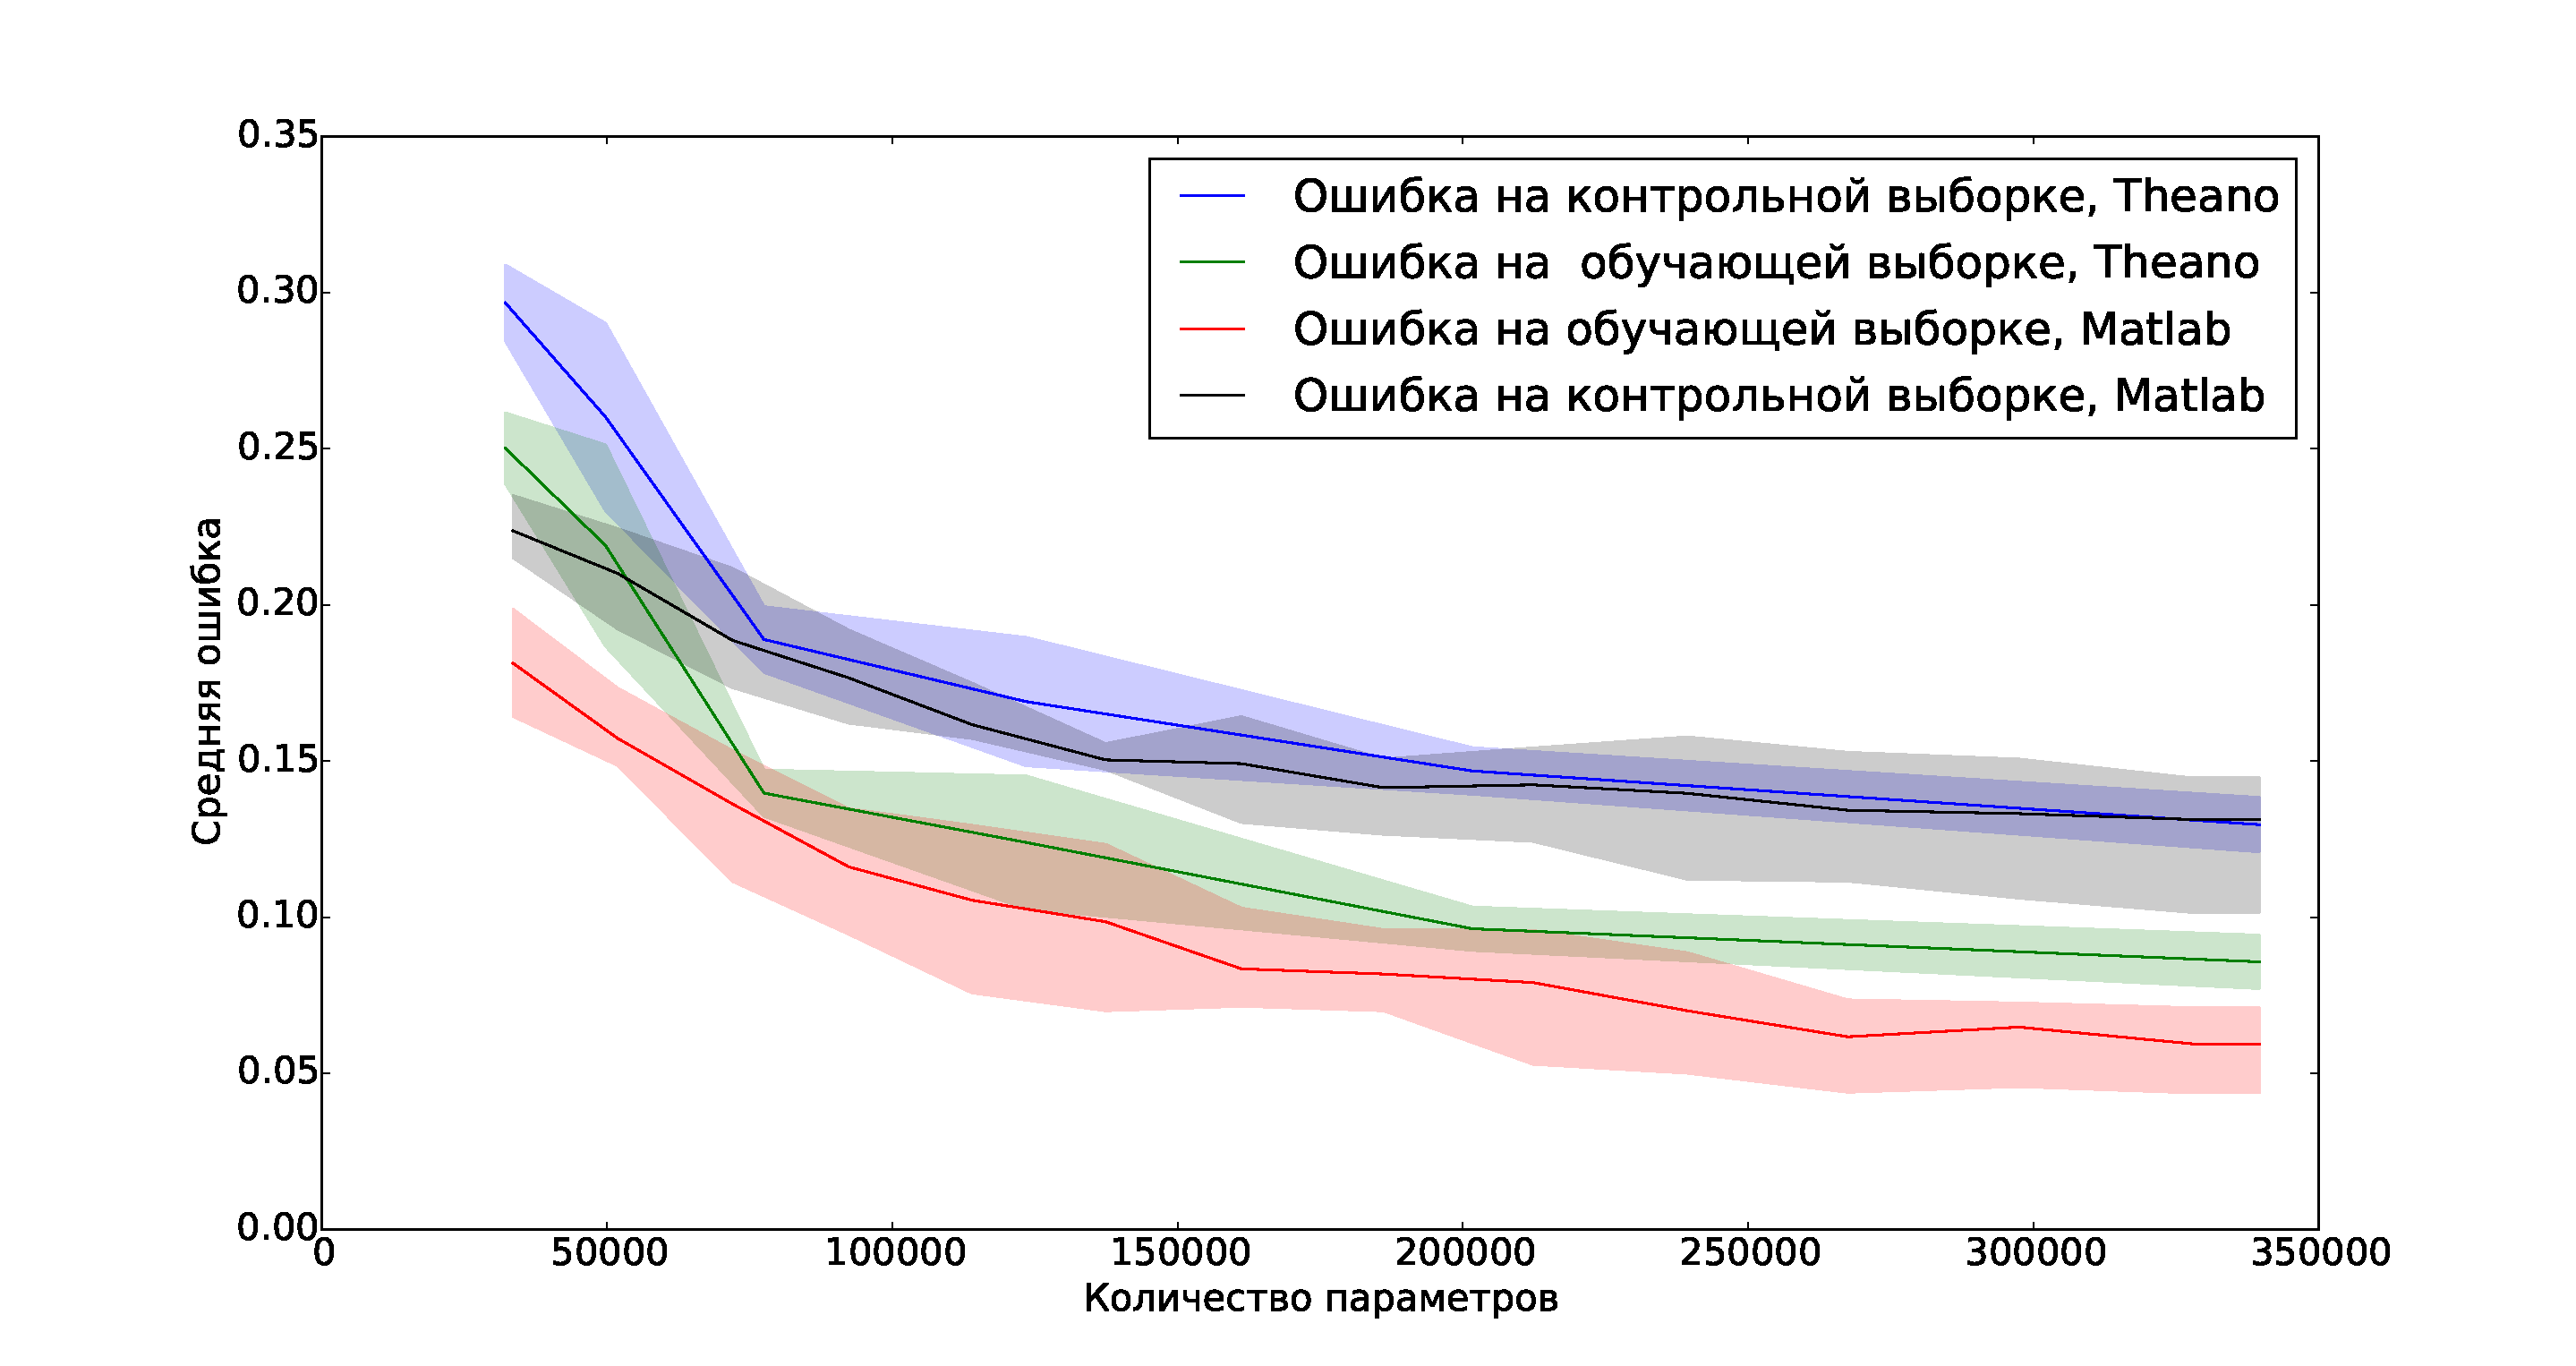
\includegraphics[width=1.0\textwidth]{plots/popova/neurons.pdf}
 \caption{Зависимость ошибки от числа нейронов}
 \label{fig:neurons}
\end{figure}


Для оценки зависимости качества классификации от размера обучающей выборки была проведена кроссвалидация с фиксированным количеством объектов в обучающей выборке (25\% исходной выборки) и переменным размером обучающей выборки. Число нейронов было установлено как 364:224:112. При проведении процедуры скользящего контроля для каждого отсчета было произведено пять запусков. График зависимости ошибки классификации от размера обучающей выборки представлен на рис.~\ref{fig:samples}.


\begin{figure}[tb!]
 \centering
  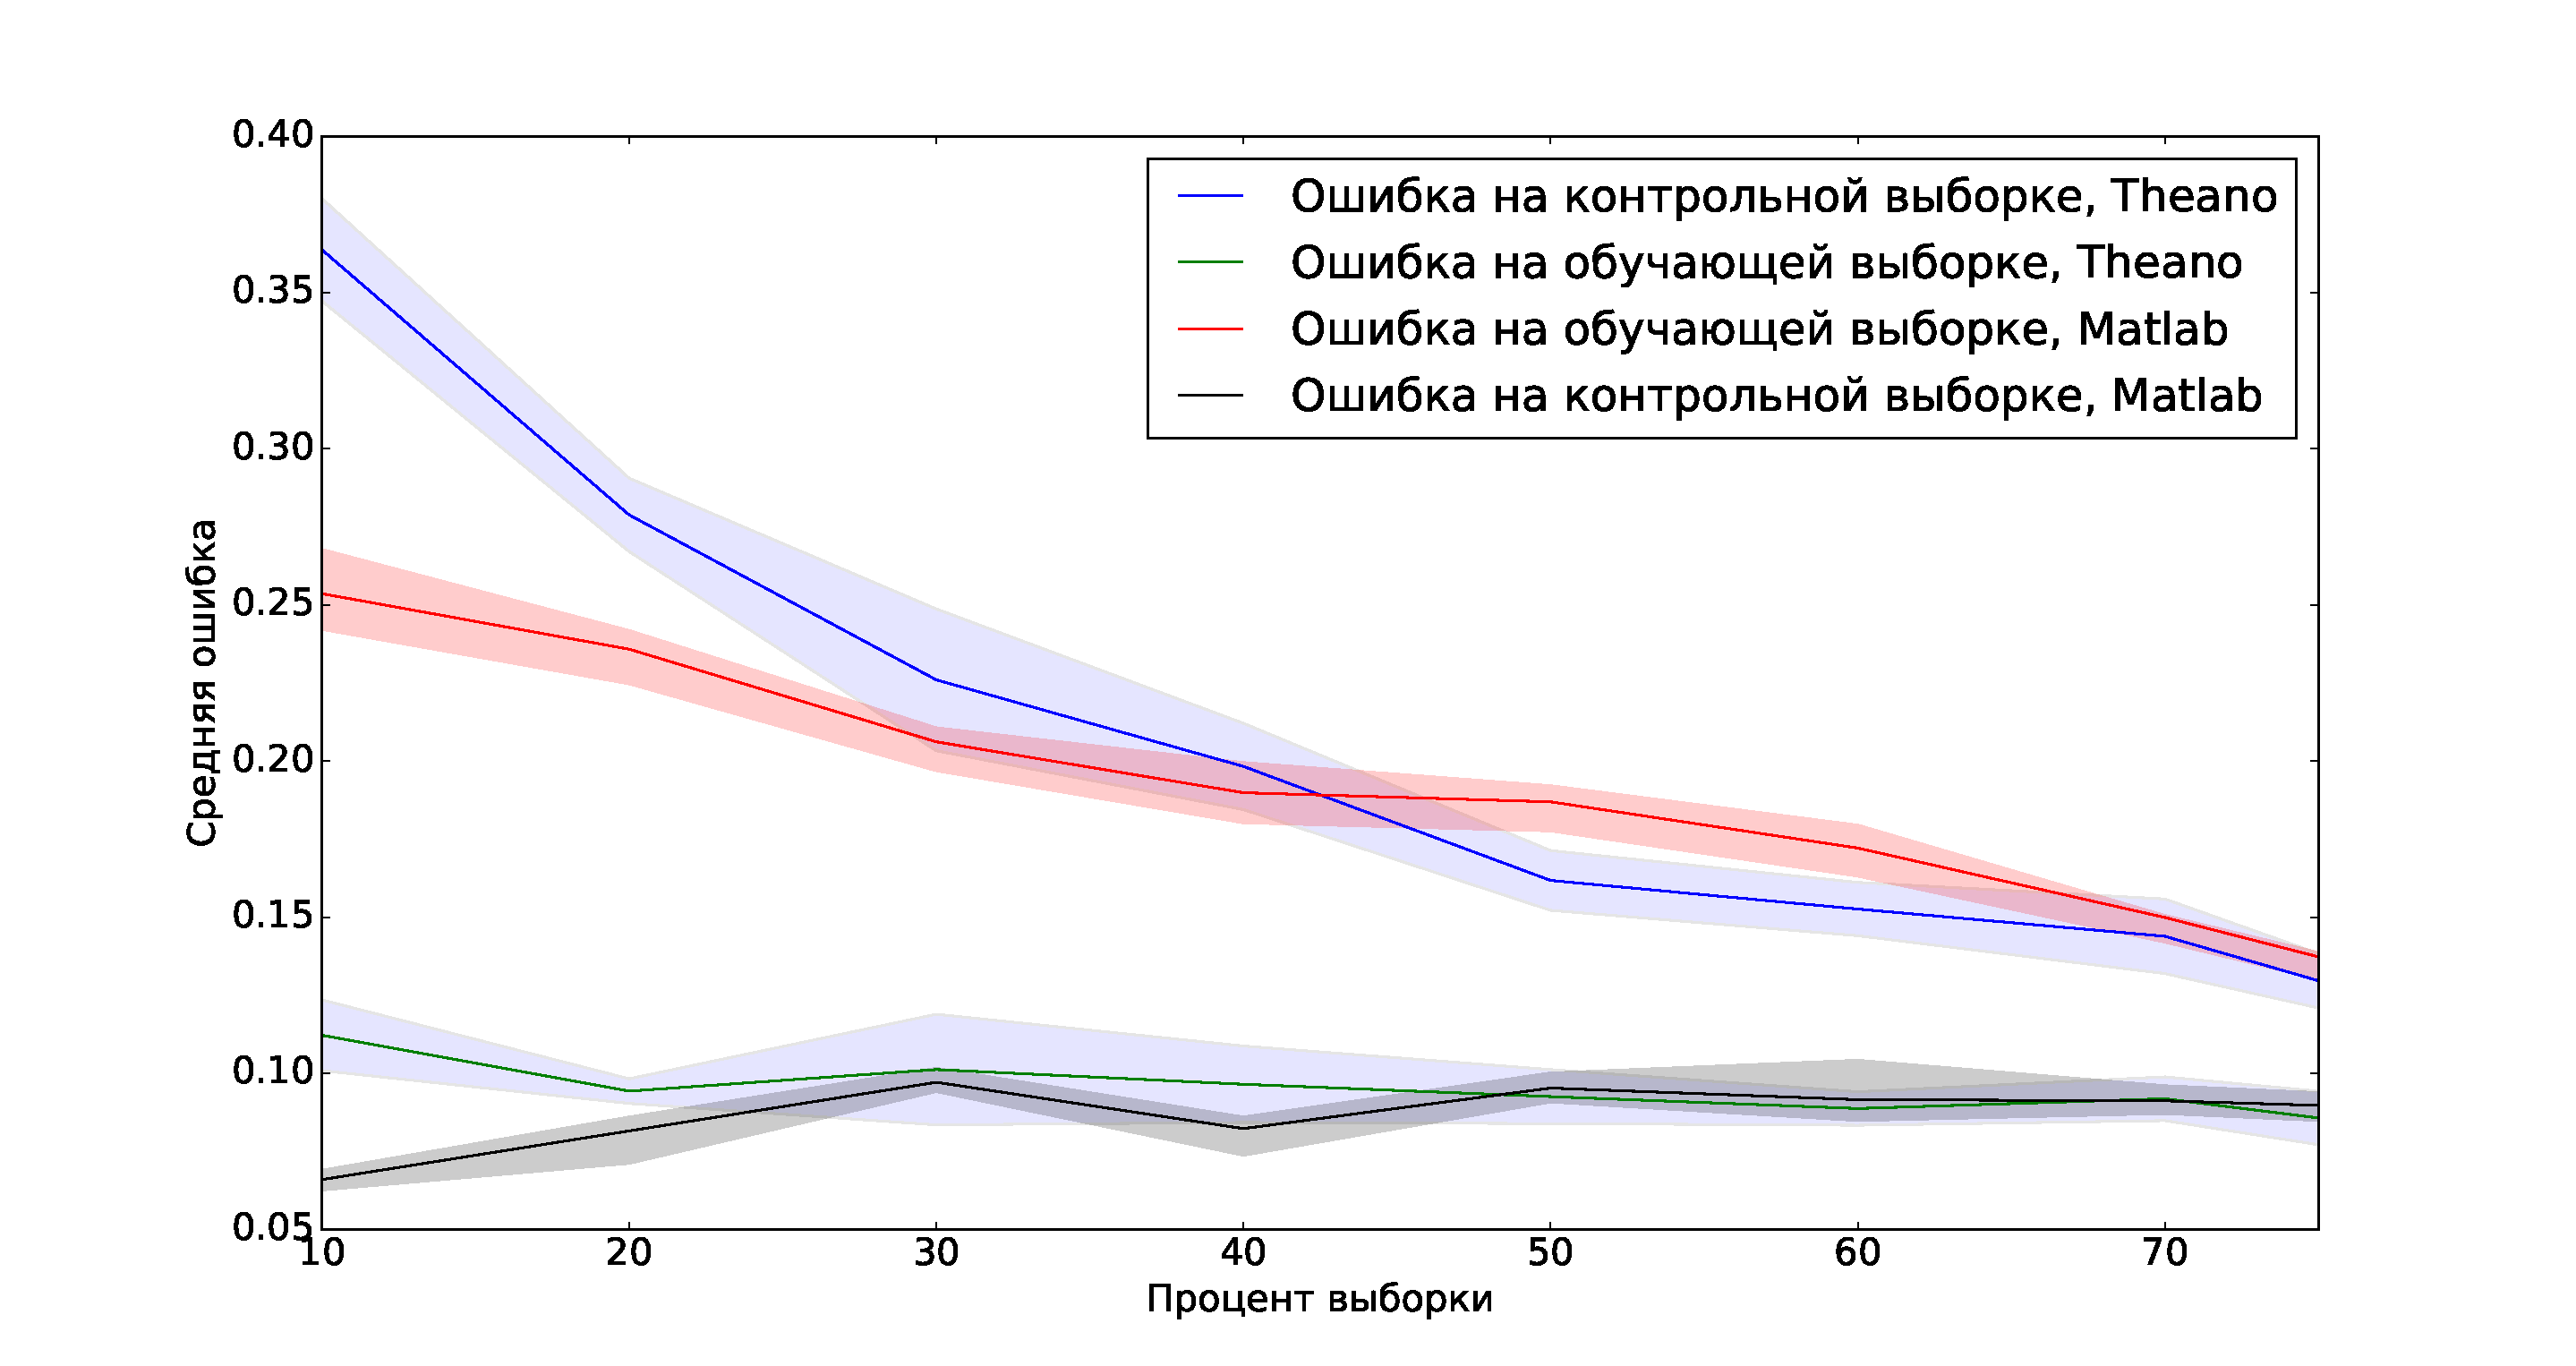
\includegraphics[width=1.0\textwidth]{plots/popova/samples.pdf}
 \caption{Зависимость ошибки от размера обучающей выборки}
 \label{fig:samples}
\end{figure}


Для исследования скорости оптимизации нейросети в зависимости от конфигурации Theano был сделан следующий эксперимент:
проводилось обучение двухслойной нейросети на основе подсчитанных заранее параметров ограниченной машины Больцмана~\eqref{eq:rbm} и автокодировщика~\eqref{eq:ae}. Обучение проходило за 100 итераций. При обучении алгоритм запускался параллельно с $r$ разными стартовыми позициями, $r \in \{1,\dots,4\}.$ Число нейронов было установлено как 300:200:100.
Запуск осуществлялся со следующими конфигурациями Theano:
\begin{itemize}
\item вычисление на центральном процессоре, задействовано
одно ядро;
\item вычисление на центральном процессоре, задействовано четыре ядра;
\item вычисление на центральном процессоре, задействовано восемь ядер;
\item вычисление на графическом процессоре.
\end{itemize}

Результаты эксперимента приведены на рис.~\ref{fig:speed}. Как видно из графика, вычисление с использованием CUDA показывает значительное ускорение по сравнению с вычислением на центральном процессоре.

\begin{figure}[tb!]
 \centering
  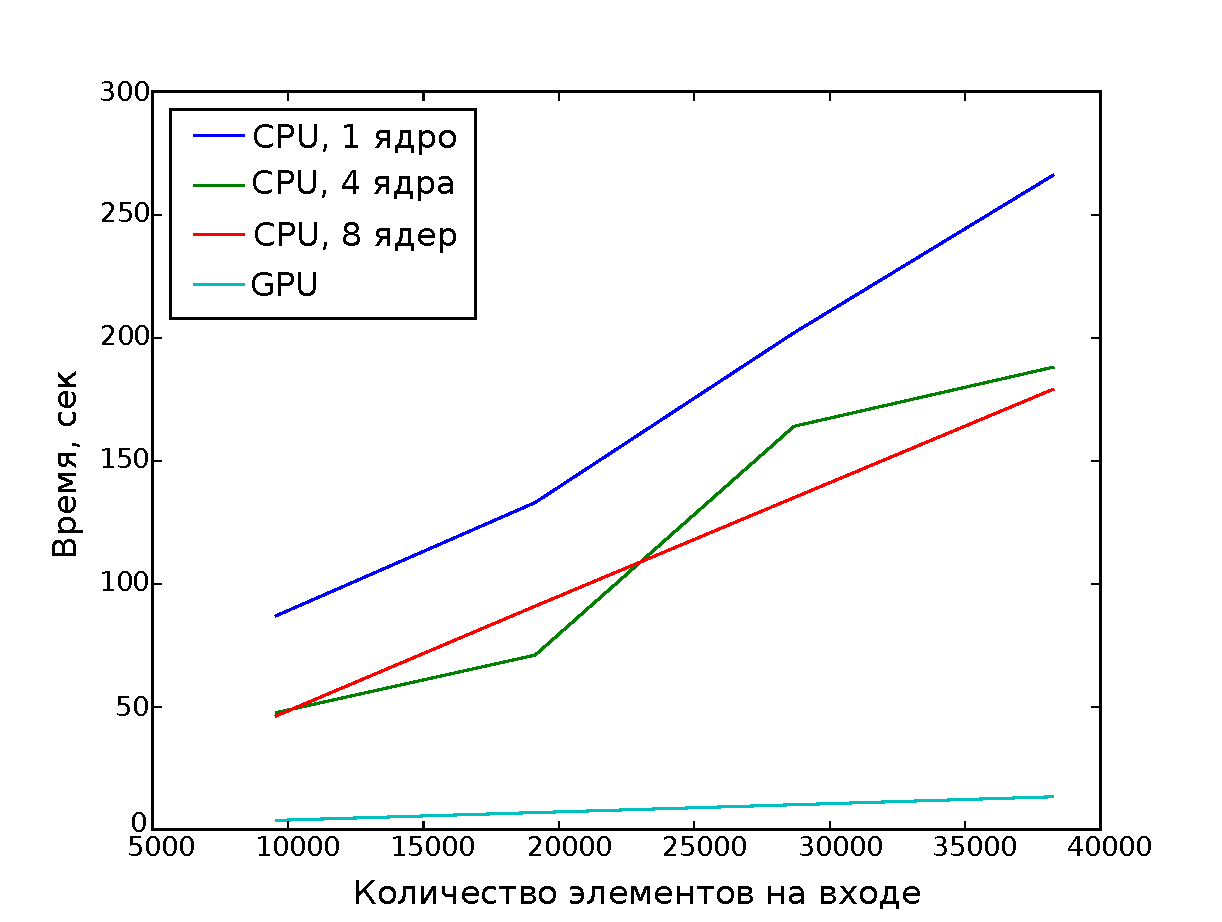
\includegraphics[width=0.8\textwidth]{plots/popova/result.pdf}
 \caption{Результаты эксперимента по исследованию скорости процесса обучения}
 \label{fig:speed}
\end{figure}




\section{Модели парафраза (Смердов)}
Цель эксперимента~--- проверка работоспособности предложенного алгоритма и сравнение результатов с ранее полученными. В качестве данных использовалась выборка SemEval 2015, состоящая из 8331 пары схожих и несхожих предложений. Слова преобразовывались в векторы размерности 50 при помощи алгоритма GloVe~\cite{GloveURL}.
%\footnote{https://github.com/stanfordnlp/GloVe}
Для базовых алгоритмов тренировочная, валидационная и тестовая выборки составили 70\%, 15\% и 15\% соответственно.
Для рекуррентной нейронной сети, полученной вариационным методом, валидационная выборка отсутствовала, а тренировочная и тестовая выборки составили 85\% и 15\% соответственно.
Критерием качества была выбрана F1-мера.
В качестве базовых алгоритмов использовались линейная регрессия, метод ближайших соседей, решающее дерево и модификация метода опорных векторов SVC. Базовые алгоритмы взяты из библиотеки sklearn. 
%\cite{sklearn}.
%\footnote{http://scikit-learn.org/stable/}.
Дополнительно были построены рекуррентная нейросеть с одним скрытым слоем~\cite{Sanborn} и нейросеть с одним скрытым слоем и вариационной оптимизацией параметров~\cite{Graves, code}.
% \footnote{https://sourceforge.net/p/mlalgorithms/code/HEAD/tree/Group474/Smerdov2017Paraphrase/code/}.

% Как показал вычислительный эксперимент, вариационная нейросеть, полученная методом, описанным в~\cite{Graves}, позволяет значительно улучшить качество предсказаний.
\begin{figure}[!h]
	\centering
	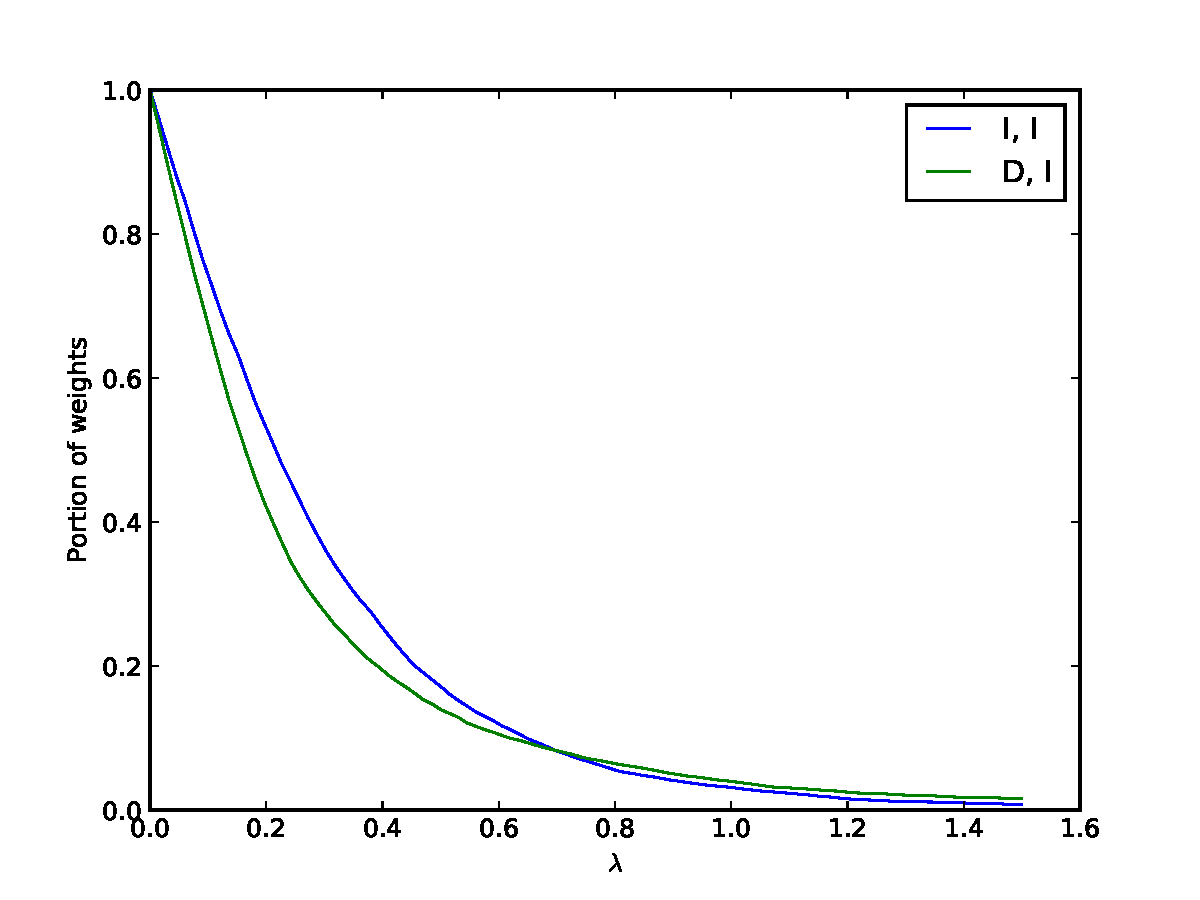
\includegraphics[width=0.5\textwidth]{plots/smerdov/lambdas.pdf}
	\caption{Доля неудаленных параметров сети в зависимости от порогового значения $\lambda$ для скалярного~($I$) и диагонального~($D$) вида апостериорной матрицы ковариаций}
	\label{lambdas}
\end{figure}

 

На рис.~\ref{evidence_I_I} и~\ref{evidence_I_D} представлена зависимость оценки правдоподобия $L$ \eqref{loss} от параметра $\lambda$.
%Видно, что существует некоторое оптимальное значения $\lambda$, при котором оценка минимальна --- именно это значение $\lambda$ соответствует оптимальной модели.
Для обоих случаев существует оптимальное значение $\lambda$, минимизирующее $L$; модели с таким параметром будут оптимальными. На рис.~\ref{score_I_I},~\ref{score_I_D},~\ref{portion_I_I} и~\ref{portion_I_D} отображены зависимости качества модели от $\lambda$ и доли выброшенных параметров. Видно, что даже при удалении большинства параметров из сети качество предсказаний меняется несущественно, что говорит о слишком большом числе параметров исходной модели.

Из рис.~\ref{lambdas} видно, что при малых $\lambda$ из сети с диагональной апостериорной матрицей ковариаций удаляется больше весов, а при больших $\lambda$ --- меньше, что говорит о лучшем отборе параметров такой моделью.


\section{Прореживание модели (Грабовой)}
Для анализа свойств предложенного алгоритма и сравнения его с существующими был проведен вычислительный эксперимент в котором параметры нейросети удалялись методами,  которые были описаны в разделах 3.1---3.3 и методом Белсли.

В качестве данных использовались три выборки. Выборки Wine~\cite{Wine} и Boston~Housing~\cite{Boston}  --- это реальные данные. Синтетические данные сгенерированы таким образом чтобы параметры сети были мультиколинеарными. Генерация данных состояла из двух этапов. 
На первом этапе генерировался вектор параметров $\mathbf{w}_{\text{synthetic}}$:
$$\mathbf{w}_{\text{synthetic}}  \sim \mathcal{N}(\textbf{m}_{\text{synthetic}}, \textbf{A}_{\text{synthetic}}), \eqno(5.1)$$ 
где 
$\textbf{m}_{\text{synthetic}} = \begin{bmatrix}
1.0\\
0.0025\\
\cdots\\
0.0025
\end{bmatrix}$,
$\textbf{A}_{\text{synthetic}} = \begin{bmatrix}
1.0& 10^{-3}& \cdots& 10^{-3}& 10^{-3}\\
10^{-3}& 1.0& \cdots& 0.95& 0.95\\
\cdots&\cdots&\cdots&\cdots&\cdots\\
10^{-3}& 0.95& \cdots& 0.95& 1.0
\end{bmatrix}$.

На втором этапе генерировалась выборка $\mathfrak{D}_{\text{synthetic}}$:
$$\mathfrak{D}_{\text{synthetic}} = \{(\textbf{x}_i,y_i)| \textbf{x}_i \sim  \mathcal{N}(\textbf{1}, \textbf{I}), y_i = x_{i0}, i = 1 \cdots 10000\}. \eqno(5.2)$$
В приведенном выше векторе параметров $\mathbf{w}_{\text{synthetic}}$ для выборки $\mathfrak{D}_{\text{synthetic}}$, наиболее релевантным является первый параметр, а все остальные параметры являются нерелевантными. Матрица ковариации была выбрана таким образом, чтобы все нерелевантные параметры были зависимы и метод Белсли был максимально эффективен.



\begin{table}[h]

\begin{center}
\caption{Описание выборок}
\begin{tabular}{|c|c|c|c|}
\hline
	Выборка &Тип задачи& Размер выборки& Число признаков\\
	\hline
	
	\multicolumn{1}{|l|}{Wine}
	&
	\multicolumn{1}{|l|}{класификация}
	 & 178 & 13\\
	\hline
	
	\multicolumn{1}{|l|}{Boston Housing}
	&
	\multicolumn{1}{|l|}{регресия}
	& 506 & 13\\
	\hline
	
	\multicolumn{1}{|l|}{Synthetic data}
	&
	\multicolumn{1}{|l|}{регресия}
	& 10000 & 100\\
\hline

\end{tabular}
\end{center}
\end{table}



Для алгоритмов тренировочная и тестовая выборки составили~$80\%$ и~$20\%$ соответсвенно. Критерием качества прореживания служит процент параметров нейросети, удаление которого не влечет значимой потери качества прогноза. Также критерием качества служит устойчивость нейросети к зашумленности данных. 

Качеством прогноза $R_{\text{cl}}$ модели для задачи классификации является точность прогноза модели:
$$R_{\text{cl}} = \frac{\sum_{(\textbf{x},y)\in \mathfrak{D}} [f(\textbf{x}, \textbf{w}) = y]}{\left|\mathfrak{D}\right|}, \eqno(5.3)$$

Качеством прогноза $R_{\text{rg}} $ модели для задачи регрессии является среднеквадратическое отклонение результата модели от точного:

$$R_{\text{rg}} = \frac{\sum_{(\textbf{x},y)\in \mathfrak{D}} \left(f(\textbf{x}, \textbf{w}) - y\right)^2}{\left|\mathfrak{D}\right|}, \eqno(5.4)$$

\textbf{Wine.} Рассмотрим нейроную сеть с 13 нейронами на входе, 13 нейронами в скрытом слое и 3 нейронами на выходе.

\begin{figure}[h!t]\center
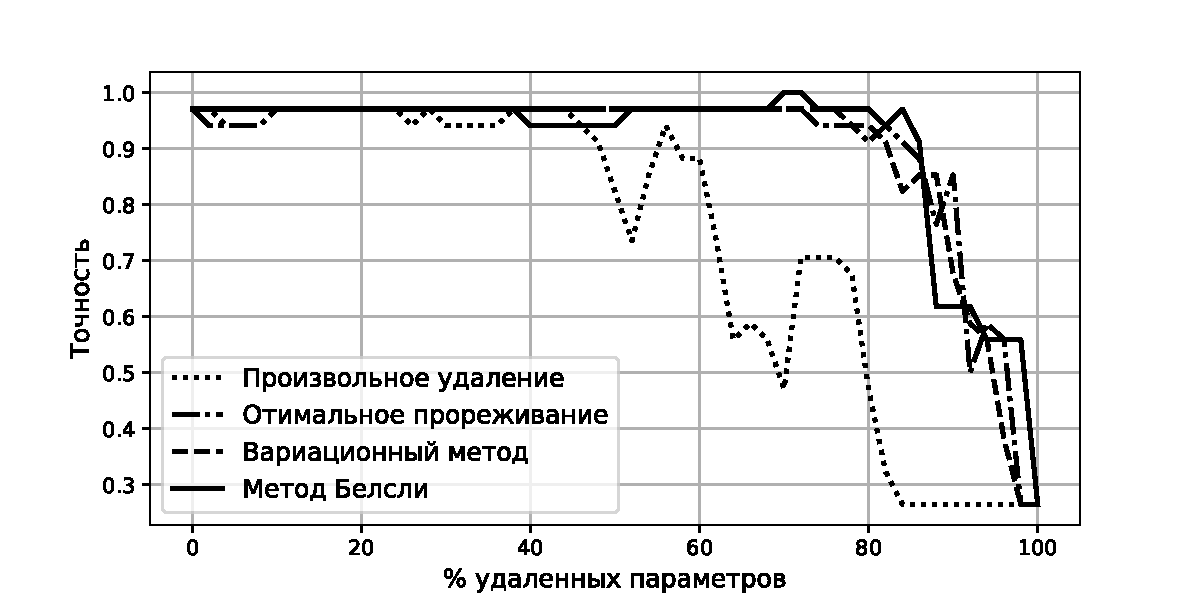
\includegraphics[width=0.8\textwidth]{plots/grabovoy/wine_all.pdf}\\
\caption{Качество прогноза при удаление параметров на выборке Wine}
\label{WineAll}
\end{figure}

\begin{figure}[ht]\center
%\begin{subfigure}[а]{0.33\textwidth}
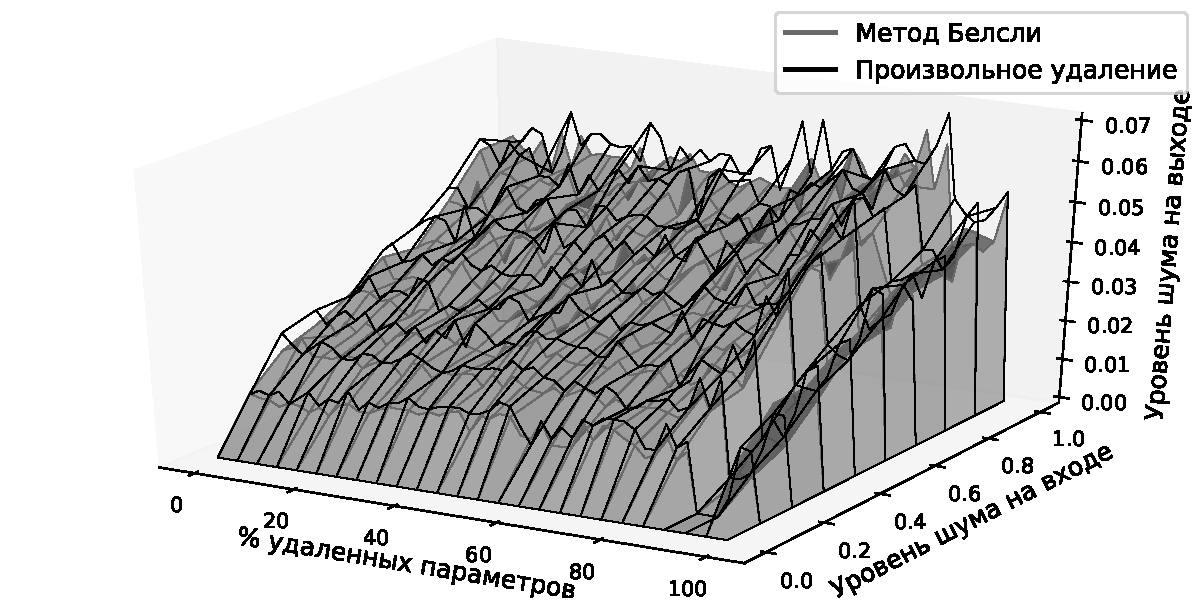
\includegraphics[width=0.33\textwidth]{plots/grabovoy/wine_random_noise3d.pdf}
%\end{subfigure}
%\begin{subfigure}[б]{0.33\textwidth}
{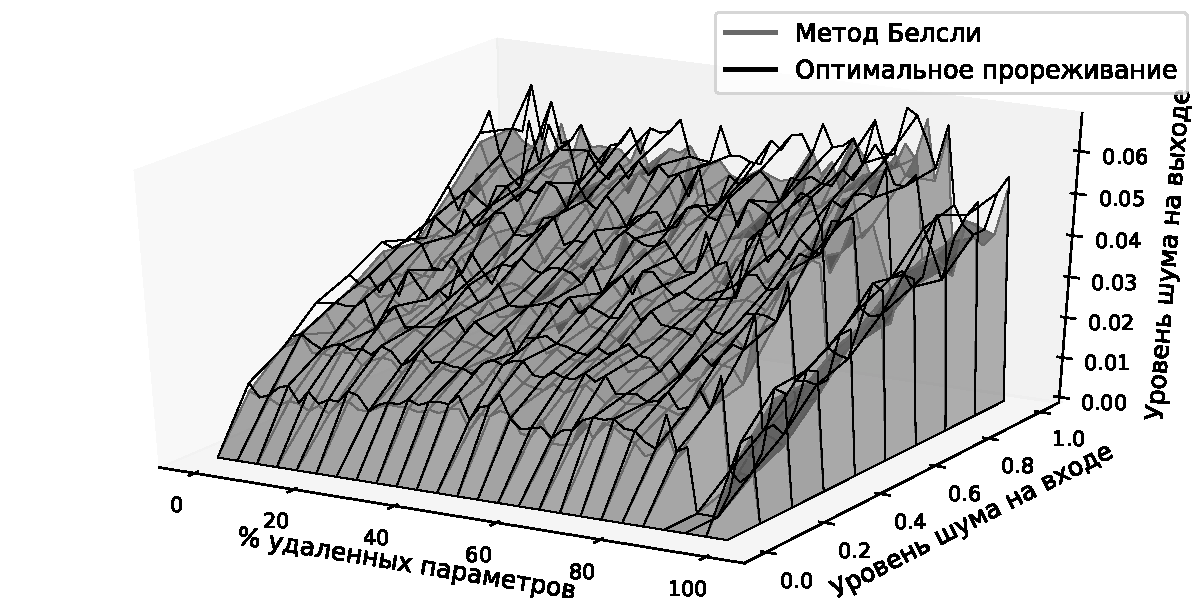
\includegraphics[width=0.33\textwidth]{plots/grabovoy/obd_noise_3d.pdf}}
%\end{subfigure}
%\begin{subfigure}[в]{0.33\textwidth}
{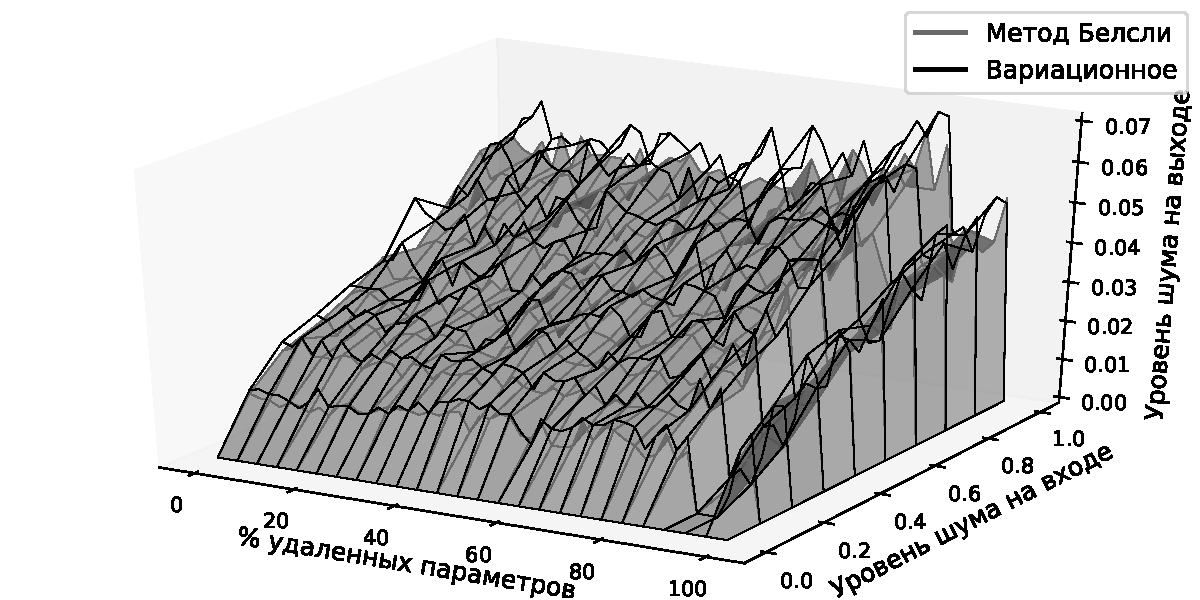
\includegraphics[width=0.33\textwidth]{plots/grabovoy/var_noise_3d.pdf}}
%\end{subfigure}

%\subfigure[Оптимальное прореживание]{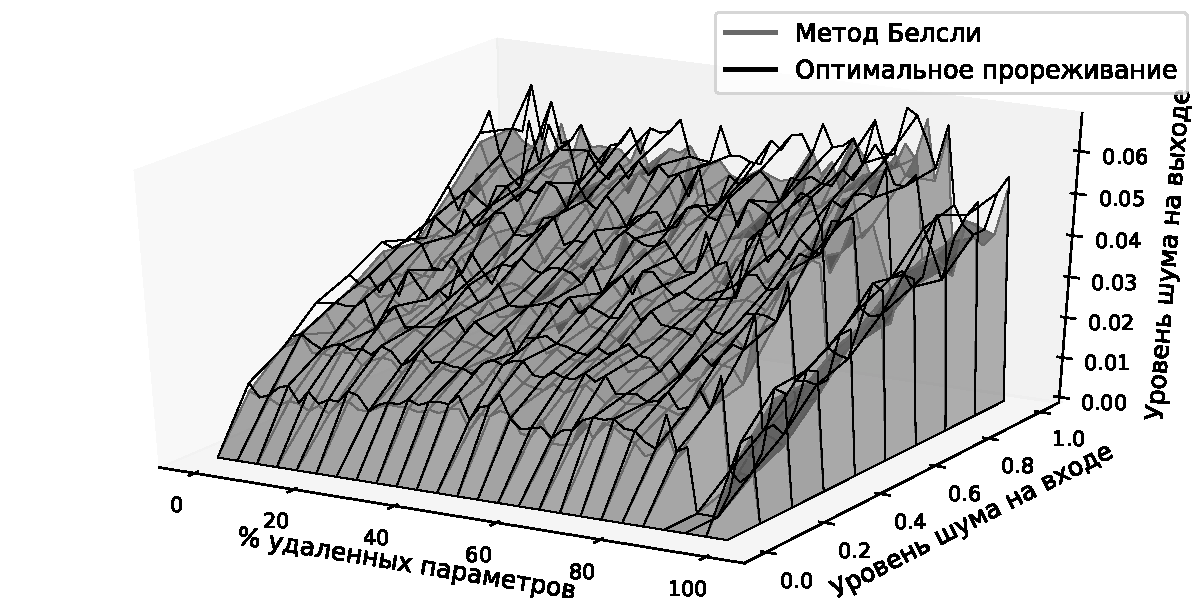
\includegraphics[width=0.5\textwidth]{plots/grabovoy/obd_noise_3d.pdf}}\\
%\subfigure[Вариационный метод]{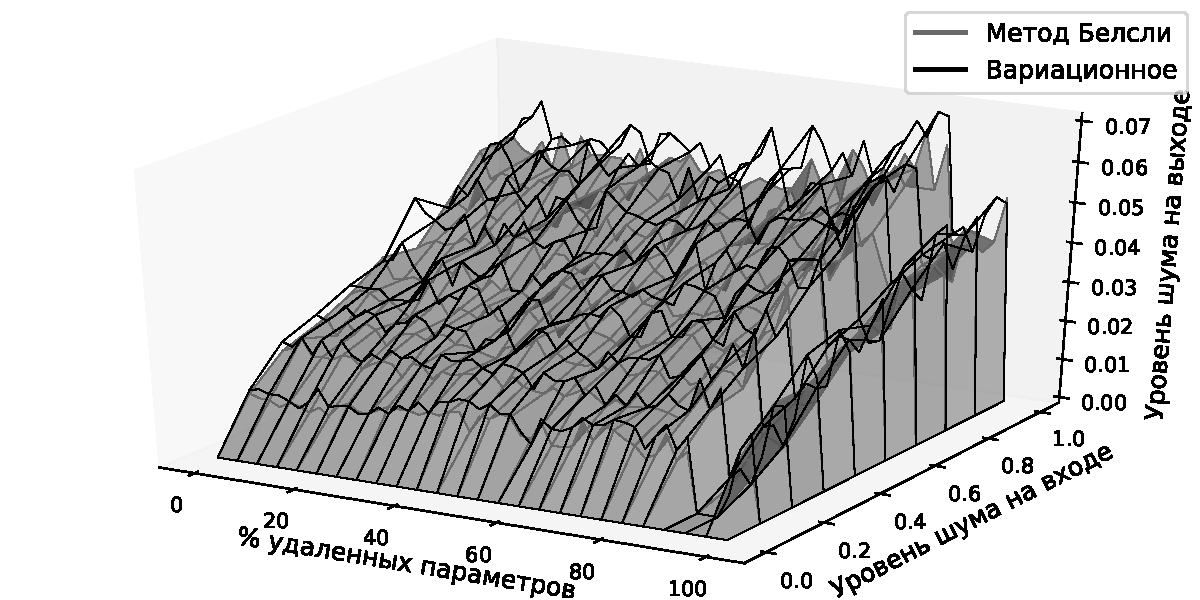
\includegraphics[width=0.5\textwidth]{plots/grabovoy/var_noise_3d.pdf}}
\caption{Влияние шума в начальных данных на шум выхода нейросети на выборке Wine: a --- Произвольное удаление параметров, б --- Оптимальное прореживание, в --- Вариационный метод}
\label{WineNoise}
\end{figure}

На рис.~\ref{WineAll} показано как меняется точность прогноза $R_{\text{cl}}$ при удалении параметров указанными методами. Из графика видно, что метод оптимального прореживания, вариационный метод и метод Белсли позволяют удалить $\approx80\%$ параметров и качество всех этих методов падает при удалении $\approx90\%$ параметров нейросети. 

На рис.~\ref{WineNoise} показаны поверхности изменения уровня шума ответов нейросети при изменении процента удаленных параметров и уровня шума входных данных для разных методов прореживания. На графиках показано, что при удалении параметров нейросети методом Белсли шум меньше, чем при удалении параметров другими методами, на это указывает то что поверхность которая соответствует методу Белсли ниже других поверхностей.

\textbf{Boston Housing. } Рассмотрим нейроную сеть с 13 нейронами на входе, 39 нейронами в скрытом слое и одним нейроном на выходе.

\begin{figure}[h    !t]\center
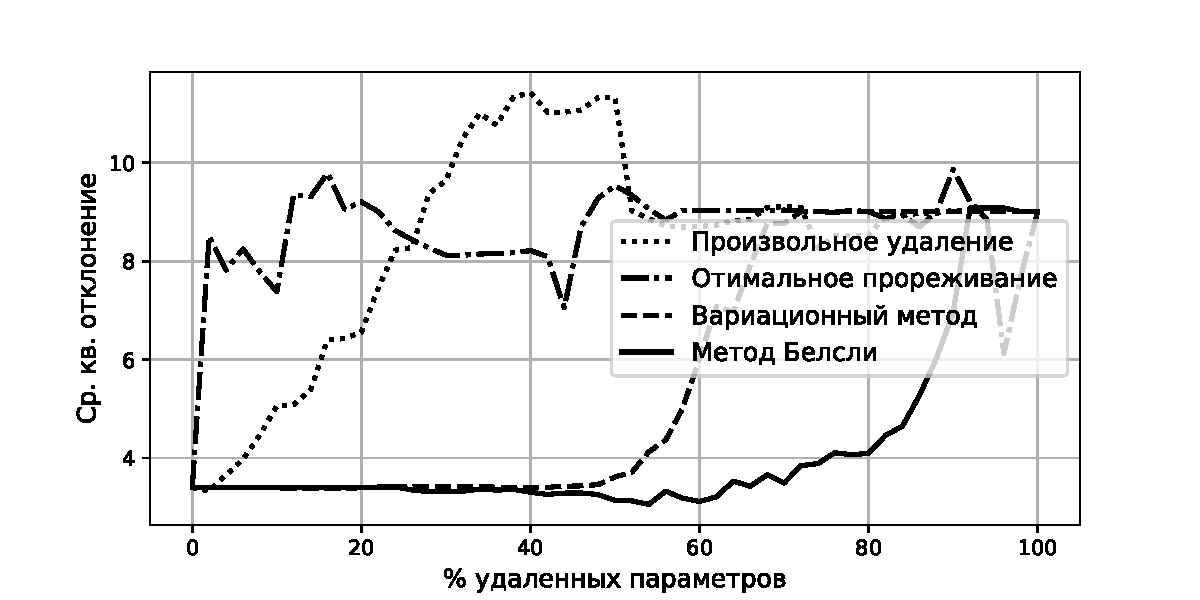
\includegraphics[width=0.8\textwidth]{plots/grabovoy/boston_all.pdf}\\
\caption{Качество прогноза при удаление параметров на выборке Boston}
\label{BostonAll}
\end{figure}



\begin{figure}[ht]\center
%\begin{subfigure}[а]{0.33\textwidth}
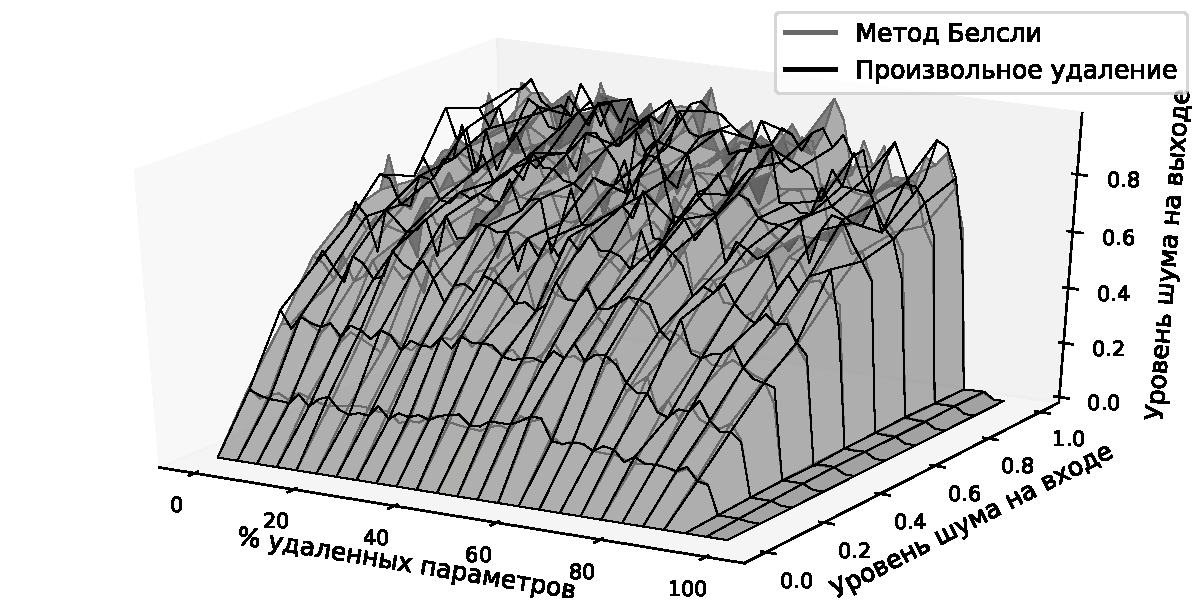
\includegraphics[width=0.33\textwidth]{plots/grabovoy/boston_random.pdf}
%\end{subfigure}
%\begin{subfigure}[б]{0.33\textwidth}
{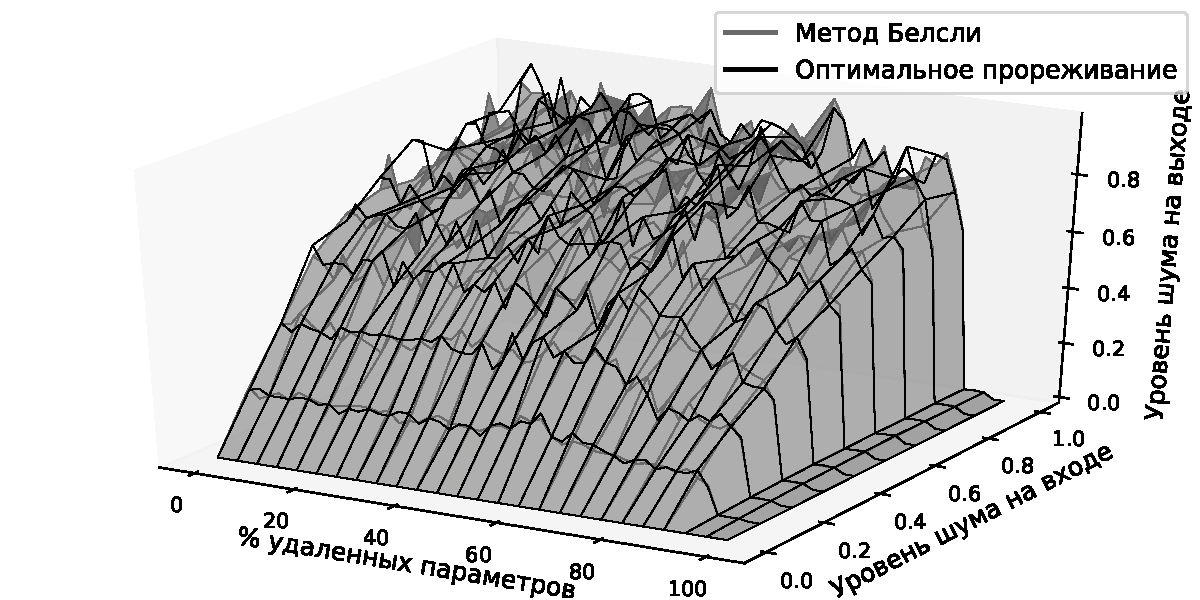
\includegraphics[width=0.33\textwidth]{plots/grabovoy/boston_obd.pdf}}
%\end{subfigure}
%\begin{subfigure}[в]{0.33\textwidth}
{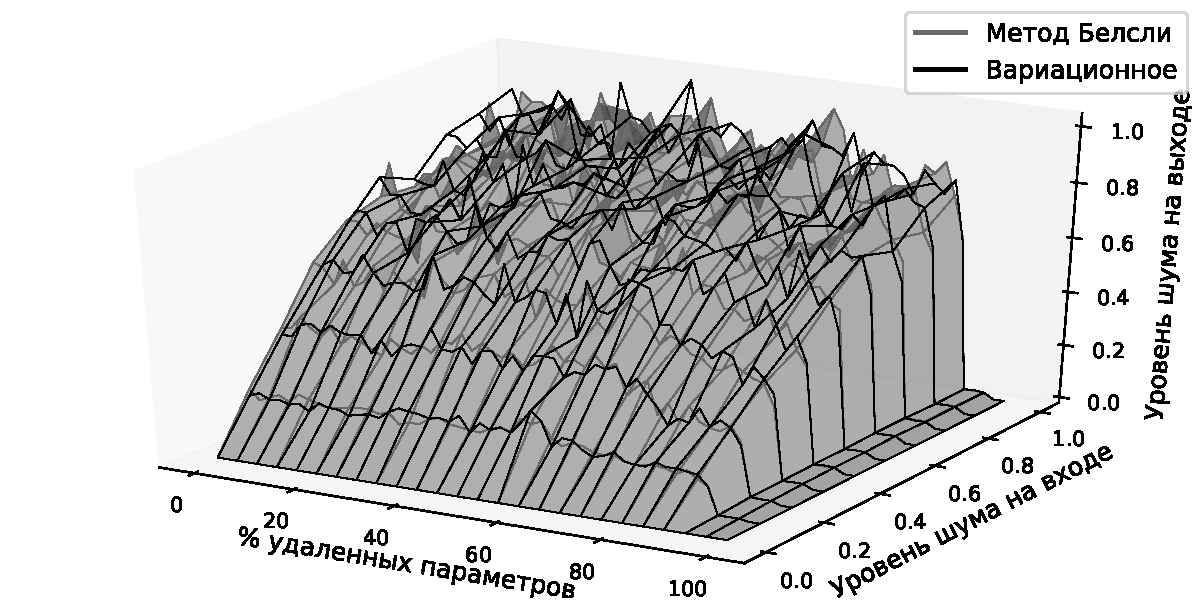
\includegraphics[width=0.33\textwidth]{plots/grabovoy/boston_var.pdf}}
%\end{subfigure}

%\subfigure[Оптимальное прореживание]{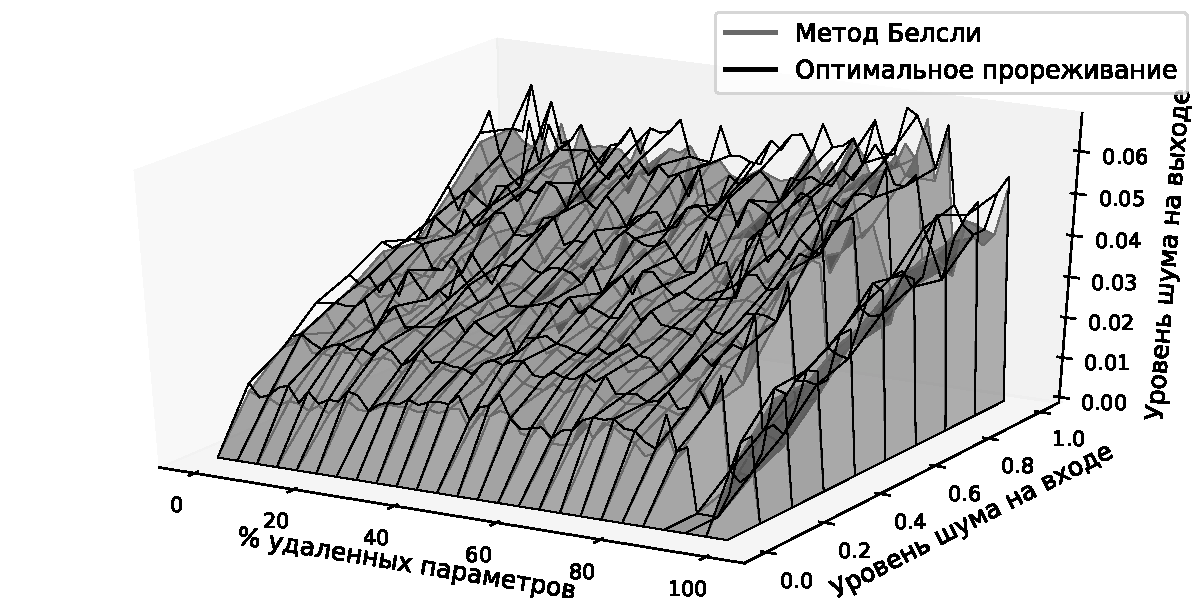
\includegraphics[width=0.5\textwidth]{plots/grabovoy/obd_noise_3d.pdf}}\\
%\subfigure[Вариационный метод]{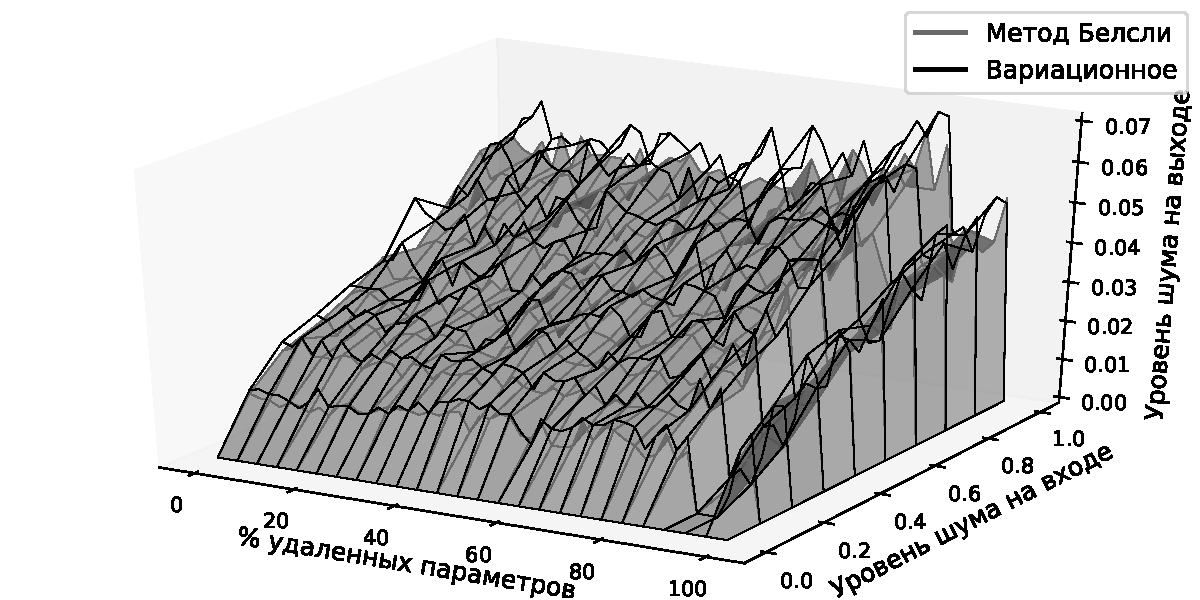
\includegraphics[width=0.5\textwidth]{plots/grabovoy/var_noise_3d.pdf}}
\caption{Влияние шума в начальных данных на шум выхода нейросети на выборке Boston: a --- Произвольное удаление параметров, б --- Оптимальное прореживание, в --- Вариационный метод}
\label{BostonNoise}
\end{figure}

На рис.~\ref{BostonAll} показано как меняется среднеквадратическое отклонение прогноза $\mathsf{R}_{\text{rg}}$ от точного ответа  при удалении параметров указанными методами. График показывает, что метод Белсли является более эффективным, чем другие методы, так-как позволяет удалить больше параметров нейросети без потери качества.

На рис.~\ref{BostonNoise} показаны поверхности изменения уровня шума ответов нейросети при изменении процента удаленных параметров и уровня шума входных данных для разных методов прореживания. График показывает, что уровень шума всех методов одинаковый, так-как поверхности всех методов находятся на одном уровне.


\textbf{Синтетические данные. } Рассмотрим нейроную сеть с 100 нейронами на входе и одним нейроном на выходе.

\begin{figure}[h!t]\center
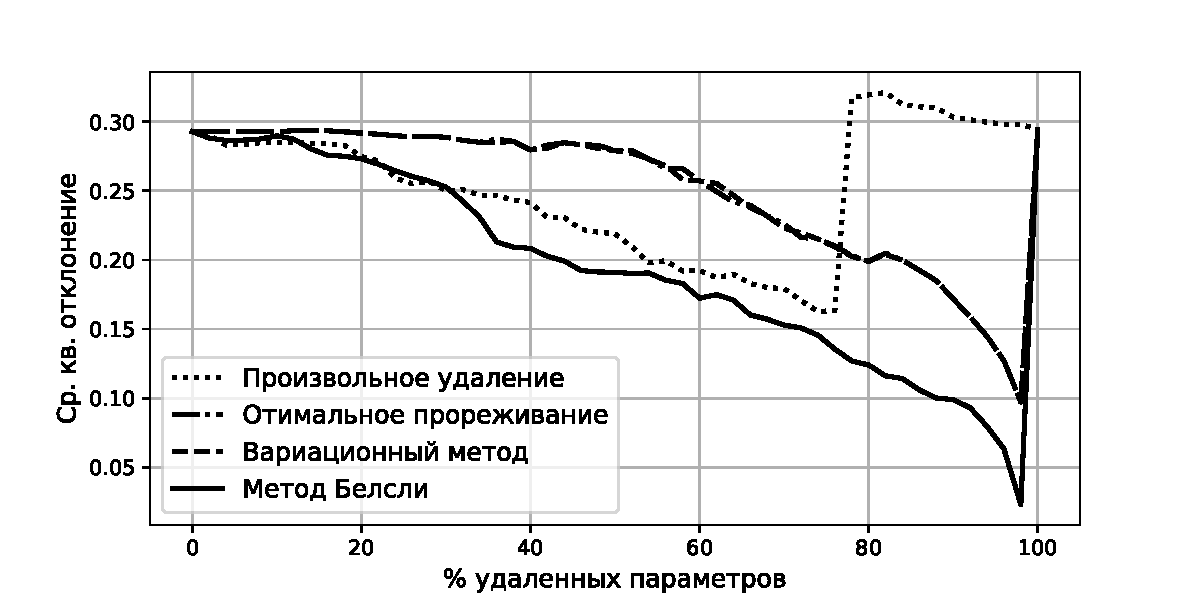
\includegraphics[width=0.8\textwidth]{plots/grabovoy/synt_all.pdf}\\
\caption{Качество прогноза при удаление параметров на синтетической выборке}
\label{Data1All}
\end{figure}

\begin{figure}[ht]\center
%\begin{subfigure}[а]{0.33\textwidth}
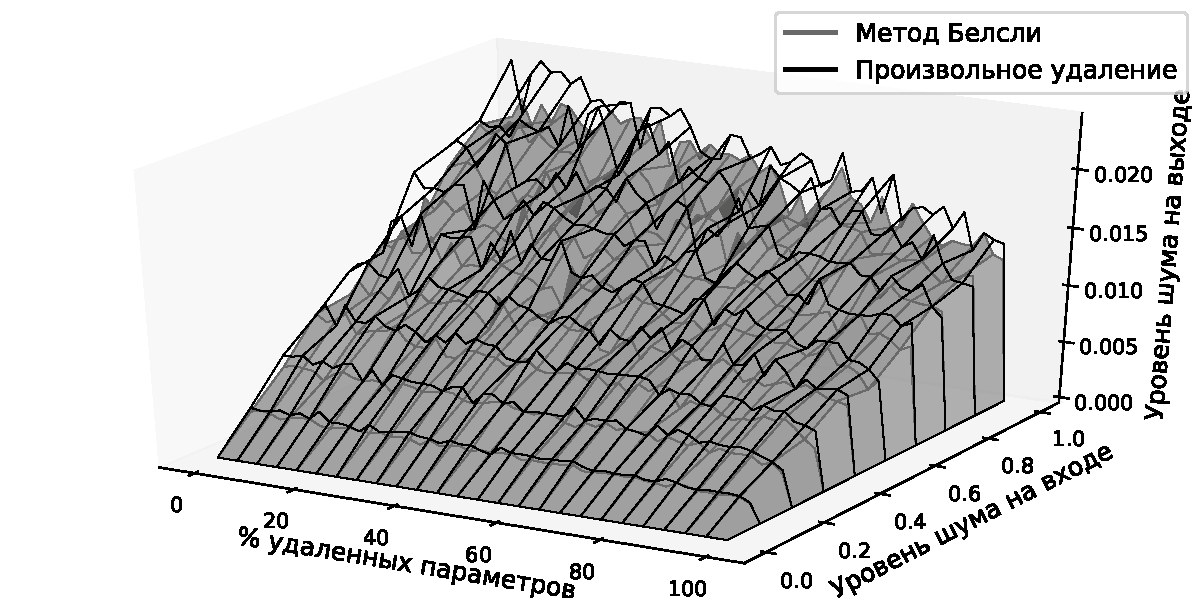
\includegraphics[width=0.33\textwidth]{plots/grabovoy/synt_random.pdf}
%\end{subfigure}
%\begin{subfigure}[б]{0.33\textwidth}
{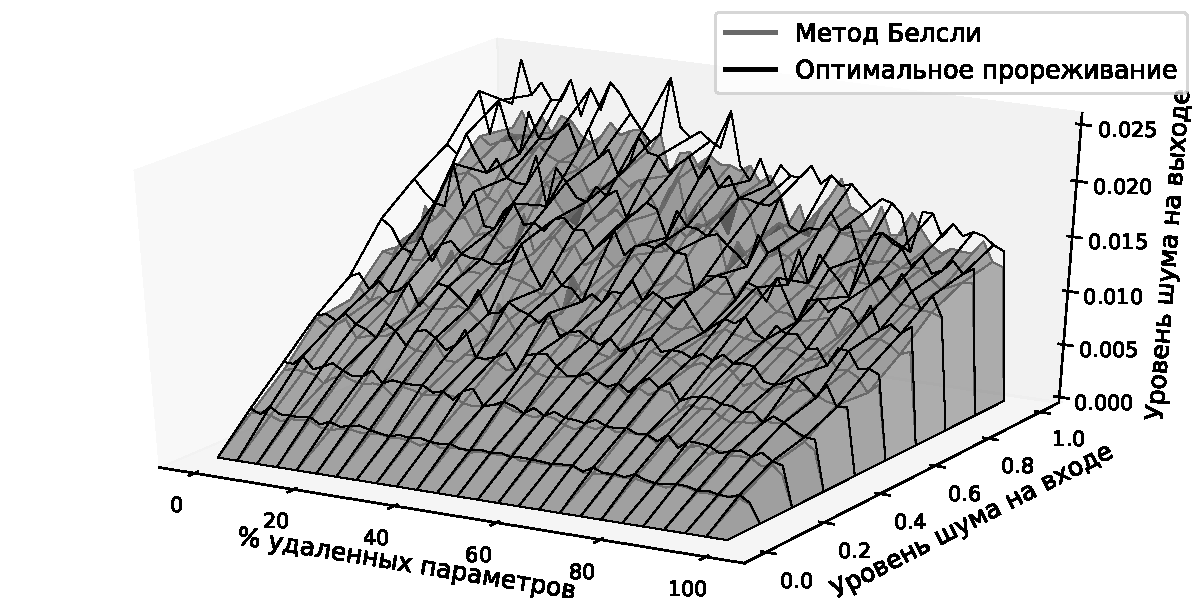
\includegraphics[width=0.33\textwidth]{plots/grabovoy/synt_obd.pdf}}
%\end{subfigure}
%\begin{subfigure}[в]{0.33\textwidth}
{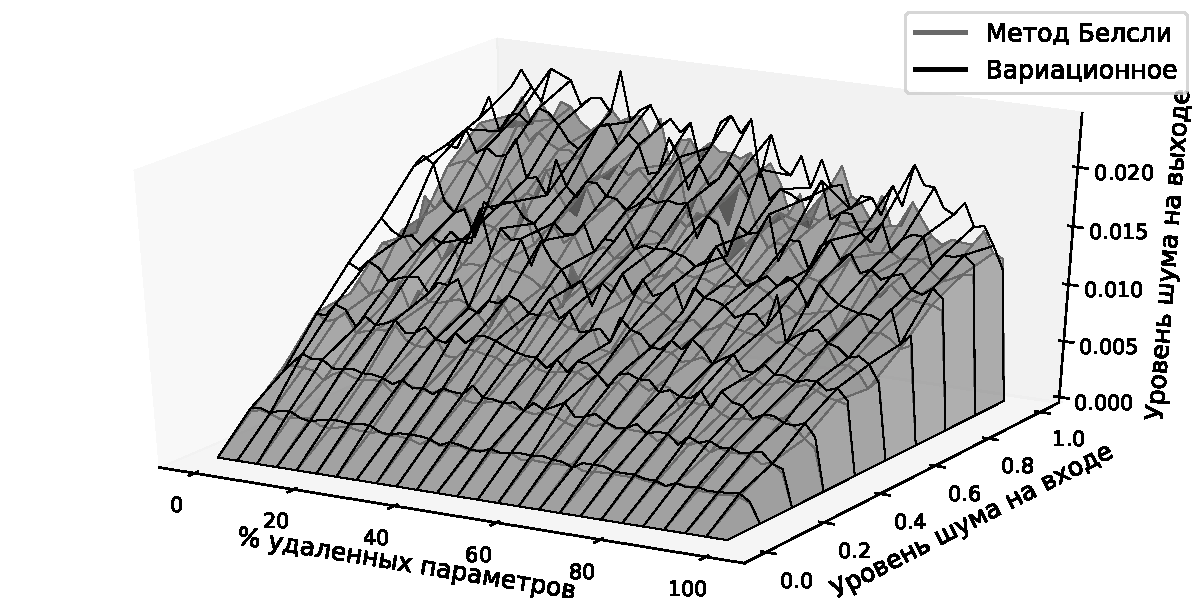
\includegraphics[width=0.33\textwidth]{plots/grabovoy/synt_var.pdf}}
%\end{subfigure}

%\subfigure[Оптимальное прореживание]{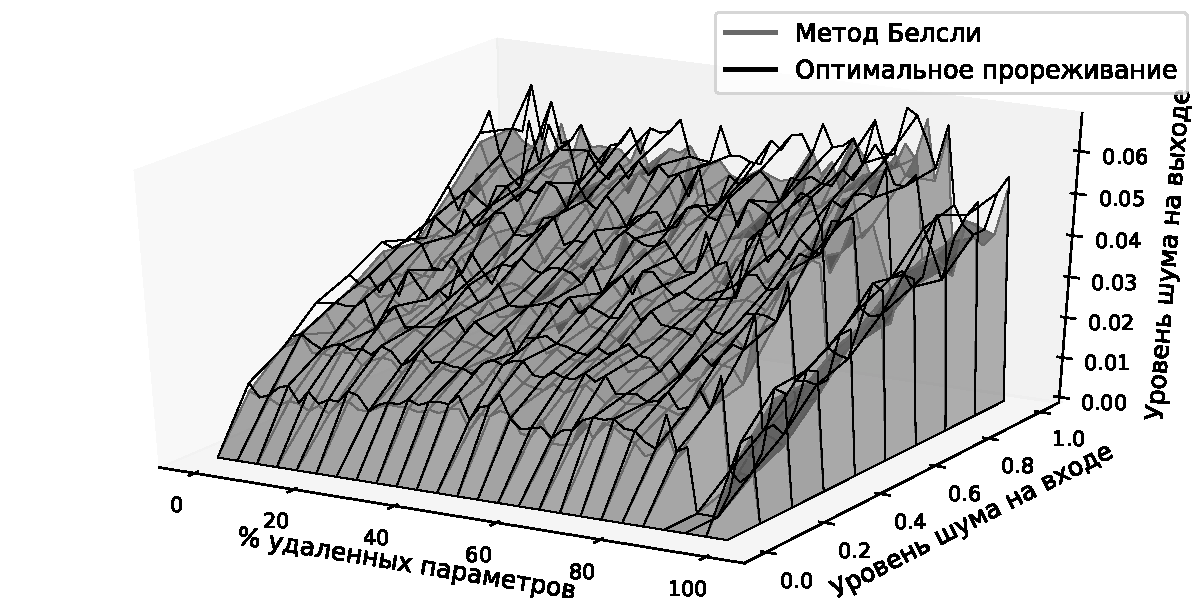
\includegraphics[width=0.5\textwidth]{plots/grabovoy/obd_noise_3d.pdf}}\\
%\subfigure[Вариационный метод]{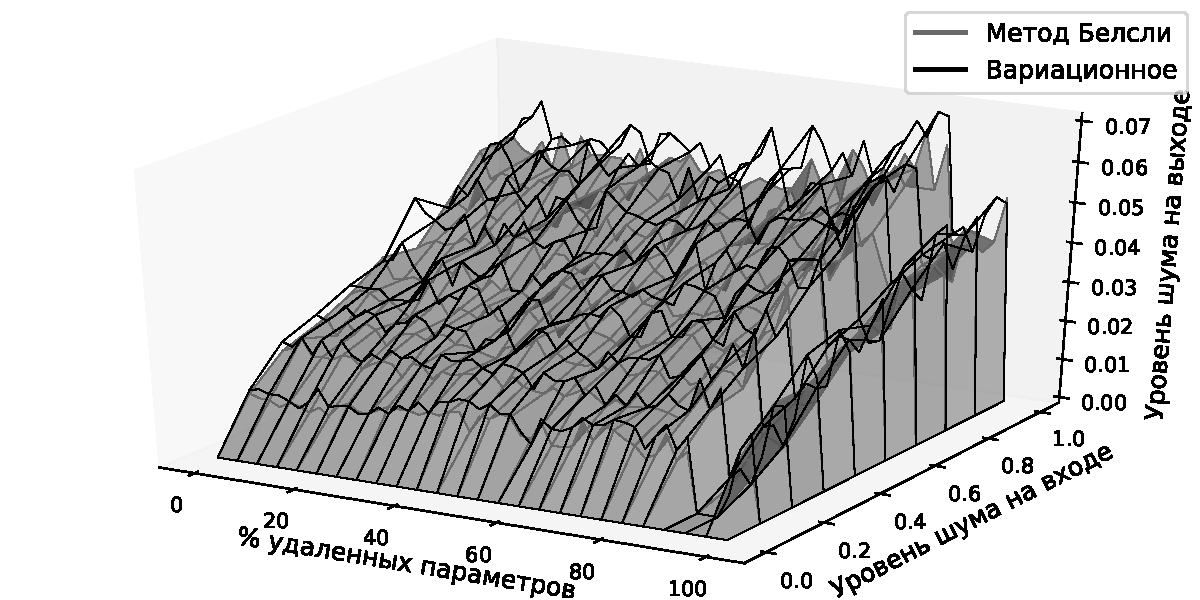
\includegraphics[width=0.5\textwidth]{plots/grabovoy/var_noise_3d.pdf}}
\caption{Влияние шума в начальных данных на шум выхода нейросети на выборке Boston: a --- Произвольное удаление параметров, б --- Оптимальное прореживание, в --- Вариационный метод}
\label{Data1Noise}
\end{figure}
На рис.~\ref{Data1All} показано как меняется среднеквадратическое отклонение прогноза от $\mathsf{R}_{\text{rg}}$ точного ответа при удалении параметров указанными методами. График показывает, что удаление параметров методом Белсли являеться более эффективным чем другие методы прореживания, так-как качество прогноза нейросети улучшается при удалении шумовых параметров.

На рис.~\ref{Data1Noise} показаны поверхности изменения уровня шума ответов нейросети при изменении процента удаленных параметров и уровня шума входных данных для разных методов прореживания. На графиках показано, что при удалении параметров нейросети методом Белсли шум меньше, чем при удалении параметров другими методами, так-как поверхность которая соответствует методу Белсли ниже других поверхностей.






\clearpage
\addcontentsline{toc}{section}{Заключение}

\chapter*{Заключение}
В работе были предложены критерии оптимальной и субоптимальной сложности моделей глубокого обучения. Предложен алгоритм выбора субоптимальной модели, основанный на получении вариационной нижней оценки  правдоподобия модели. Был предложен метод получения оценки, основанный на стохастическом градиентном спуске, позволяющий проводить выбор модели и оптимизацию модели единообразно. Исследованы свойства стохастического градиентного спуска, а также оценок правдоподобия, полученных с его использованием. 
Работа представленного алгоритма проиллюстрирована рядом выборок. 
Вычислительный эксперимент продемонстрировал значимое влияние априорного распределения на апостериорное распределение параметров модели. В силу многоэкстремальности оптимизируемых функций получение аналитических оценок для гиперпараметров модели является вычислительно сложным. В дальнейшем  планируется исследовать применение 
предложенных алгоритмов для оптимизации гиперпараметров градиентными методами, представленными в~\cite{hyper}.






The experiments showed that each algorithm can perform effectively and therefore the appropriate hyperparameter optimization method should rely on the amount of hyperparameters and the specific of the problem. 

When dealing with small amount of hyperparameters the random search showed the best results since the search procedure can be employed more effectively than gradient-based optimization in low-dimensional hyperparameters space. For the high-dimensional hyperparameter space both the  HOAG and greed algorithms showed good performance. 
The HOAG algorithm is more preferable if the model optimization problem is expensive. On the other hand we can schedule greed hyperparameter optimization to make it less expensive as in~\cite{greed_hyper}. 

The DrMad algorithm showed rather poor results on the MNIST and WISDM datasets. Perhaps it is because of high learning rate $\gamma$ we used in experiments. The large value of the learning rate can make the DrMad algorithm instable. Two improvements can be proposed. We can use more stable optimization like Adam or AdaGrad for both parameter and hyperparameter optimization. The second improvement was proposed to develop in~\cite{hyper_mad}: we can use more complicated parameter trajectory approximation to make it more similar to the original parameter trajectory. Opposing to the HOAG and greedy algorithms, the DrMad optimization has prerequisites for optimization not only hyperparameters but also the metaparameters, i.e. the parameters  of the optimization procedure. The opportunity of such optimization using reversed differentiation was shown in~\cite{hyper_mad}. 

The other interesting aspect of our experiments is the relation between the model error (RMSE or Accuracy) and the value of validation loss $Q$. The models obtained by the evidence lower bound showed higher errors than the models obtained using cross-validation on the MNIST and WISDM datasets. Nevertheless these models also showed greater stability when the noise was added to the Test datasets.  The evidence lower bound showed significantly better results on the synthetic dataset, when the amount of object in the Train dataset is small. Therefore we can conclude that the evidence lower bound usage is preferable when the model tend to overfit or when the cross-validation usage is too computationally expensive.   In~\cite{nips} note that the evidence lower bound optimization required more iterations for the convergence. In our experiments we used the same number of iterations both for the cross-validation and evidence lower bound. The more accurate iteration number calibration can improve the final quality of these models. 


The paper analyzed the gradient-based hyperparameter optimization algorithms. We adapted the analyzed algorithms for general validation functions and evaluated their performance on the  MNIST and WISDM datasets. Two model selection criteria were compared: the cross-validation and evidence lower bound. 

The experiments showed that the gradient-based algorithms are effective when the number of hyperparameters is large. The results showed that models obtained using evidence lower bound have higher error rater than models obtained using cross-validation, but they are also more stable when the test dataset contain a lot of noise. 

The authors  implemenetd the algorithms as a toolbox available at~\cite{pyfos}. The toolbox is developed in Python using Theano~\cite{theano} and Numpy~\cite{numpy} libraries. 

In the future we are planning to develop the analyzed algorithm and to extend gradient-based algorithms to optimize not only hyperparameters, but also the parameters of the model optimization. The other object of our research will be the difference between the cross-validation and evidence lower bound and the theoretical aspects of their properties for the models with large amount of parameters.




\clearpage


\addcontentsline{toc}{chapter}{Список оcновных обозначений}
\chapter*{Список оcновных обозначений}
\noindent$\mathbf{x}_i$ --- вектор признакового описания $i$-го объекта\\
$y_i$ --- метка $i$-го объекта\\
$\mathfrak{D}$ --- выборка\\
$\mathbf{X}$ --- матрица, содержащая признаковое описание объектов выборки\\
$\mathbf{y}$ --- вектор меток объектов выборки\\
$m$ --- количество объектов в выборке\\
$n$ --- количество признаков в признаковом описании объекта\\
$\mathbb{X}$ --- признаковое пространство объектов\\
$\mathbb{Y}$ --- множество меток объектов\\
$Z$ --- множество классов в задаче классификации\\
$(V,E)$ --- граф со множеством вершин $V$ и множеством ребер $E$\\
$\mathbf{g}^{j,k}$ --- вектор базовых функций для ребра $(j,k)$\\
$K^{j,k}$ --- мощность вектора базовых функций для ребра $(j,k)$\\
$\textbf{agg}_v$ --- функция аггрегации для вершины $v$. 
$\boldsymbol{\gamma}^{j,k}$ --- структурный параметр для ребра $(j,k)$\\
$\Delta^{K}$ --- симплекс на $K$ вершинах\\
$\bar{\Delta}^{K}$ --- множество вершин симплекса на $K$ вершинах\\
$\mathfrak{F}$ --- семейство моделей\\
$\mathbf{W}$ --- параметры модели\\
$\mathbb{W}$ --- пространство параметров модели\\
$\boldsymbol{\Gamma}$ --- структура модели\\
$\mathbb{\Gamma}$ --- множество значений структуры модели\\
$\mathbf{h}$ --- гиперпараметры модели\\
$\mathbb{H}$ --- пространство гиперпараметров модели\\
$p(\mathbf{W}, \boldsymbol{\Gamma}|\mathbf{h})$ --- априорное распределение параметров и структуры модели\\
$p(\mathbf{W}, \boldsymbol{\Gamma}|\mathbf{y}, \mathbf{X}, \mathbf{h})$ --- апостериорное распределение параметров и структуры модели\\
$p({y}, \mathbf{W},  \boldsymbol{\Gamma}|\mathbf{x}, \mathbf{h})$ --- вероятностная модель глубокого обучения\\
$p(y|\mathbf{X}, \mathbf{W}, \boldsymbol{\Gamma})$ --- правдоподобие выборки\\
$p(y|\mathbf{X}, \mathbf{h})$ --- правдоподобие модели\\
$q(\mathbf{W}, \boldsymbol{\Gamma})$ --- аппроксимирующее распределение\\
$\boldsymbol{\theta} \in \mathbb{R}^u$ --- оптимизируемые параметры модели\\
$L(\mathbf{X}, \mathbf{y},\boldsymbol{\theta}, \mathbf{h})$ --- функция потерь\\
$Q(\mathbf{X}, \mathbf{y}, \boldsymbol{\theta}, \mathbf{h})$ --- валидационная функция\\
$T(L, \mathbf{y}, \mathbf{X}, \boldsymbol{\theta}, \mathbf{h}, \boldsymbol{\beta})$ --- оператор оптимизации\\
$\boldsymbol{\beta}$ --- вектор метапараметров\\

\clearpage 
 
\addcontentsline{toc}{section}{Список иллюстраций}
\listoffigures

\clearpage
\addcontentsline{toc}{section}{Список таблиц}
\listoftables

\clearpage

\addcontentsline{toc}{section}{Список литературы}
\renewcommand{\bibname}{Список использованных источников}
\addcontentsline{toc}{chapter}{Список использованных источников}
\bibliographystyle{gost71u}
\bibliography{dis_literature}
\end{document}
